\documentclass[twocolumn]{aastex631}
\usepackage{graphics,graphicx}
\hypersetup{urlcolor=blue}
\usepackage{natbib}
\usepackage[outdir=./]{epstopdf}
\usepackage{textcomp,gensymb}
\usepackage{xfrac}
\usepackage{xcolor}

\newcommand{\vdag}{(v)^\dagger}
\newcommand\aastex{AAS\TeX}
\newcommand\latex{La\TeX}
\newcommand{\clustername}{MELANGE-2}

\newcommand{\name}{KOI-3876}
\newcommand{\starname}{KOI-3876}
\newcommand{\planetname}{KOI-3876\,b}
\newcommand{\koi}{3876 }
\newcommand{\ticid}{122450696}
\newcommand{\kicid}{3440118}

\newcommand{\nametwo}{Kepler-970}
\newcommand{\starnametwo}{Kepler-970}
\newcommand{\planetnametwo}{Kepler-970\,b}
\newcommand{\koitwo}{1838}
\newcommand{\ticidtwo}{???}
\newcommand{\kicidtwo}{5526527}

\newcommand\apx{\ensuremath{\sim}}
\newcommand\citeeg[1]{\csitep[\emph{e.g.},][]{#1}}
\renewcommand\deg{\ensuremath{^\circ}}
\newcommand\dm[1]{\ensuremath{{\rm DM}_{\rm #1}}}
\newcommand\dmu{cm$^{-3}$~pc}
\newcommand\dt{\ensuremath{{\Delta t}}}
\newcommand\eg{\emph{e.g.}}
\newcommand\etal{\emph{et~al.}}
\newcommand\ha{\ensuremath{{\text{H}\alpha}}}
\newcommand\ie{\emph{i.e.}}
\newcommand\msun{\ensuremath{\text{M}_\odot}}
\newcommand\speclum{erg~s$^{-1}$~Hz$^{-1}$}
\newcommand\todo[1]{\textcolor{red}{#1}}
\newcommand\ujy{$\mu$Jy}
\newcommand\ujybm{$\mu$Jy/bm}
\newcommand{\mps}{m\,s$^{-1}$}
\providecommand{\icarus}{Icarus}
\newcommand{\vsini}{$v\sin{i_*}$}
\newcommand{\oxygen}{O$_2$}
\newcommand{\water}{H$_2$O}
\newcommand{\kepler}{{\it Kepler}}
\newcommand{\logg}{$log~g$ }
\newcommand{\metal}{[M/H]}
\newcommand{\av}{$A_V$}
\newcommand{\um}{$\mu$m}
\newcommand{\fbol}{$F_{\mathrm{bol}}$}
\newcommand{\mbol}{$m_{\mathrm{bol}}$}
\newcommand{\Mbol}{$M_{\mathrm{bol}}$}
\newcommand{\rapsq}{$R_{ap}^2$}
\newcommand{\rchisq}{$\chi^2_{\nu}$}
\newcommand{\hipp}{{\it Hipparcos}}
\newcommand{\teff}{\ensuremath{T_{\text{eff}}}}
\newcommand\kms{km~s$^{-1}$}
\newcommand{\ms}{m~s$^{-1}$}
\newcommand{\tess}{\textit{TESS}}
\newcommand{\ktwo}{{\textit K2}}
\newcommand{\re}{$R_{\oplus}$}
\newcommand{\gaia}{{\textit Gaia}}
\newcommand{\association}{MELANGE-2}
\newcommand{\coude}{Coud{\'e}}

%\accepted{August 10, 2020}
%\submitjournal{AJ}

\shorttitle{A mini-Pleiades in the Kepler field}
\shortauthors{Barber et al.}
\graphicspath{{./}{}}

\begin{document}

\title{Transit Hunt for Young and Maturing Exoplanets (THYME) VIII: a Pleiades-age association harboring a transiting planet from \kepler\ (NOW TWO TRANSITING SYSTEMS)}

\correspondingauthor{Madyson G. Barber}
\email{madysonb@live.unc.edu}


    
%THYME, Lead, misttborn fits, notch/locor search, PM plot, XYZ plot, rotation sequence (with JLB), significant text, corner plot for transit, transit-fit plot, radial velocity (archive), giant member table, 
\author[0000-0002-8399-472X]{Madyson G. Barber}%
\affiliation{Department of Physics and Astronomy, The University of North Carolina at Chapel Hill, Chapel Hill, NC 27599, USA} 

%THYME, Li sequence, significant text, radius/SED + fig, isochronal fit (mixture) + 2 plots, adjustments to FF plots.
\author[0000-0003-3654-1602]{Andrew W. Mann}%
\affiliation{Department of Physics and Astronomy, The University of North Carolina at Chapel Hill, Chapel Hill, NC 27599, USA} 

% %% 2.7m spectra, HRVs, Li EqW, text for HRV and Li
\author[0000-0003-2053-0749]{Benjamin M. Tofflemire}
\altaffiliation{51 Pegasi b Fellow}
\affiliation{Department of Astronomy, The University of Texas at Austin, Austin, TX 78712, USA}

% %Rotation analysis of target and friends, rotation sequence plot
\author[0000-0002-9446-9250]{Jonathan L. Bush}%
\affiliation{Department of Physics and Astronomy, The University of North Carolina at Chapel Hill, Chapel Hill, NC 27599, USA} 

% %%THYME, FF, suggestions on follow-up
\author[0000-0001-9811-568X]{Adam L. Kraus}%
\affiliation{Department of Astronomy, The University of Texas at Austin, Austin, TX 78712, USA}

% %Coude data, reduction
\author[0000-0001-9626-0613]{Daniel Krolikowski}%
\affiliation{Department of Astronomy, The University of Texas at Austin, Austin, TX 78712, USA}

% %THYME, assistance with LCs. 
\author[0000-0001-7246-5438]{Andrew Vanderburg}%
\affiliation{Department of Physics and Kavli Institute for Astrophysics and Space Research, Massachusetts Institute of Technology, Cambridge, MA 02139, USA}

% %%inclination and his stellar parameter code (mass). 
\author[0000-0002-9641-3138]{Matthew J. Fields}
\affiliation{Department of Physics and Astronomy, The University of North Carolina at Chapel Hill, Chapel Hill, NC 27599, USA} 

% %THYME
\author[0000-0003-4150-841X]{Elisabeth R. Newton}%
\affiliation{Department of Physics and Astronomy, Dartmouth College, Hanover, NH 03755, USA}

% misttborn
\author[0000-0002-6397-6719]{Dylan A. Owens}%
\affiliation{Department of Physics and Astronomy, The University of North Carolina at Chapel Hill, Chapel Hill, NC 27599, USA} 

%MOLUSC + Bib help
\author[0000-0001-7336-7725]{Mackenna L. Wood}%
\affiliation{Department of Physics and Astronomy, The University of North Carolina at Chapel Hill, Chapel Hill, NC 27599, USA} 

%% other possible authors:
%% we did use notch, but I think Aaron's gain from papers is small


\begin{abstract}
We describe a young association (\association) in the \kepler\ field with a known planet candidate (KOI-3876.01) with signs of youth. To better determine the age and membership of \association, we combine archival light curves, velocities, astrometry, with new high-resolution spectra of stars nearby KOI-3866.01 spatially and kinematically. The resulting rotation sequence, lithium levels, and color-magnitude diagram of members are all an excellent match for the Pleiades, confirming the population is co-eval and providing an age estimate of 110$\pm$10\,Myr. KOI-3876's observed properties are an excellent match to the group, confirming membership. \association\ may be part of the larger Theia 316 stream, also estimated to be $\simeq$108\,Myr. For KOI-3876, we revise the stellar and planetary parameters of the system, taking into account the newly-determined age. We fit the 4.5\,yr light curve from \kepler\ and find that KOI-3876.01 is a $2.0\pm0.1R_\oplus$ planet that orbits its star every 19.58\,days on an eccentric ($e>0.2$) orbit. KOI-3876 was previously flagged as a likely eclipsing binary, but we rule this out using radial velocities from APOGEE and statistically validate the signal as planetary in origin based on archival follow-up and its \kepler\ light curve. Given its overlap with the \kepler\ field, we expect \association\ to be valuable for studies of spot evolution on timescales of years and KOI-3876 to be a piece of the growing work on transiting planets in young stellar associations.
\end{abstract}


\keywords{exoplanets, exoplanet evolution, young star clusters- moving clusters, planets and satellites: individual (KOI3876)}

\section{Introduction}\label{sec:intro}
Stellar clusters and associations serve as critical benchmarks for stellar and planetary astrophysics. Stars in such groups formed from the same interstellar cloud, and hence share a common (or similar) age, abundance pattern, and initial space velocity. The common set of properties makes it significantly easier to assign properties to the whole population, providing age estimates that are more precise and accurate than general-purpose techniques used outside clusters \citep[e.g., Gyrochronology;][]{2007ApJ...669.1167B, vanSaders2016} and work on stars where ages are especially challenging \citep[e.g., M dwarfs;][]{2021arXiv210401232K}. Such coeval associations are therefore, ideal for how studying how stellar and planetary properties evolve with time \citep{2019ARA&A..57..227K, Mann2016b}. 

Associations within the \kepler\ field have been especially valuable for stellar and planetary astrophysics. The $\simeq$4.5\,yr baseline and precise photometry enable precise measurements of rotation periods, even at older ages \citep[e.g.,][]{Angus2015, Aigrain2015}, providing some of the best constraints we have on the rotation evolution of stars past 1\,Gyr \citep{2011ApJ...733L...9M, Curtis_stall}. The four \kepler\ clusters (NGC 6866, NGC 6811, NGC 6819, and NGC 6791) have also provided a wealth of information about stellar mass-loss \citep{2012MNRAS.419.2077M}, post-main-sequence stellar evolution \citep{2012ApJ...757..190C}, and the occurrence of planets inside clusters \citep{Meibom2013}.  

The four known clusters in the \kepler\ field are all at distances of more than 1\,kpc and ages $\gtrsim$500\,Myr. While these older ages (compared to nearby young groups) fill an important niche in stellar spin down and post-main-sequence evolution, their distance from the Sun makes it challenging to study the low-mass members and search for small planets. The \ktwo\ mission covered many younger and more nearby clusters \citep{VanCleve2016, Rizzuto2017}, but only for $\simeq$80\,days at a time. Searching for long-period planets and studying longer-term spot evolution with \ktwo\ data was therefore only possible in regions that \ktwo\ covered by multiple campaigns \citep{2021arXiv210613250R}. Additional young associations in the \kepler\ field would provide the invaluable $\simeq$4.5\,yr baseline.

The availability of precise parallaxes and proper motions for millions of stars from \gaia\ \citep{Gaia_mission2016, GaiaEDR3} has enabled the discovery of new coeval stellar associations \citep[e.g.,][]{2019A&A...622L..13M, 2021arXiv210509338K}. The \texttt{FriendFinder} code\footnote{\url{https://github.com/adamkraus/Comove}} \citep{THYMEV} was designed to take advantage of \gaia\ data, by searching for potential co-moving `friends' around a user-identified young stars. This method has already been useful in finding the 250\,Myr MELANGE-1 association \citep{THYMEV} and age-dating a planet in the Musca region of Lower-Centarus-Crux \citep{2021arXiv211009531M}. 

With the goal of finding previously undiscovered associations with transiting planets, we ran \texttt{FriendFinder} on \kepler\ objects of interest suspected to be younger than Hyades based on their lithium levels in \citet{2018ApJ...855..115B}. The most promising association was a group of stars nearby KOI-3876; the candidate members showed a color-magnitude diagram (CMD) consistent with the Pleiades (consistent with the lithium levels). Here we describe our work demonstrating that the population (\association) is a co-eval 110\,Myr group, $\simeq$300\,pc from the Sun, and harbors two transiting planetary systems (\planetname\ and \planetnametwo).

While the THYME survey was meant to focus on planets identified with \tess, \planetname\ was flagged as young by the same team and using the same methods as used extensively in the THYME and ZEIT series. Since the planet is not along the ecliptic, we opted to include it in the THYME survey series with a slight adjustment to the acronym. 

The paper is organized as follows. In Section~\ref{sec:target} we detail our initial selection of potential members of \clustername. We list the range of archival and new data taken on candidate members of \clustername\ in Section~\ref{sec:obs}. In Section~\ref{sec:cluster} we demonstrate \clustername\ is a co-eval population and derive its overall properties and basic membership. Our effort to find known and new planets in \clustername\ is described in Section~\ref{sec:search}. We derive properties of the only identified planet in the association, \planetname, in Section~\ref{sec:transit}, and statistically validate it in Section~\ref{sec:fpp}. We summarize our findings in Section~\ref{sec:summary} and briefly discuss the future utility of an association overlapping the \kepler\ field. 


\section{Target Selection}\label{sec:target}

As part of our effort to identify known planets in previously undiscovered young associations we ran the \texttt{FriendFinder} code \citep{THYMEV} on all stars identified as young based on their lithium absorption \citep{2018ApJ...855..115B}; this initial seed list included \starname. The \texttt{FriendFinder} algorithm uses \gaia\ EDR3 positions, parallaxes, and proper motions to identify stars with similar Galactic tangential velocity and $XYZ$ position to a selected input source. This required an absolute velocity for \starname, for which we used the value from APOGEE \citep[-26.79\kms,][]{2020AJ....160..120J}. 

The lithium levels suggested an age for \starname\ close to the Pleiades. Unbound or weakly bound associations $>$100\,Myr should be significantly dispersed as they orbit through the Galaxy (this needs a citation). So we used a generous selection, including any star within 5\kms\ and 50\,pc of \starname\ as a candidate member. This yielded 1007 candidates.

We show the color-magnitude diagram (CMD) for our candidate members in Figure~\ref{fig:CMD}. The spread of the CMD suggests significant contamination; it is likely that most of the 1007 stars selected are not associated with \starname. However, the CMD also shows  there is significant contamination, there is also a sequence of the closest stars (in tangential velocity) consistent with the Pleiades single-star sequence. This matches the age suggested by the Li levels in \starname.


\begin{figure*}[tb]
    \centering
    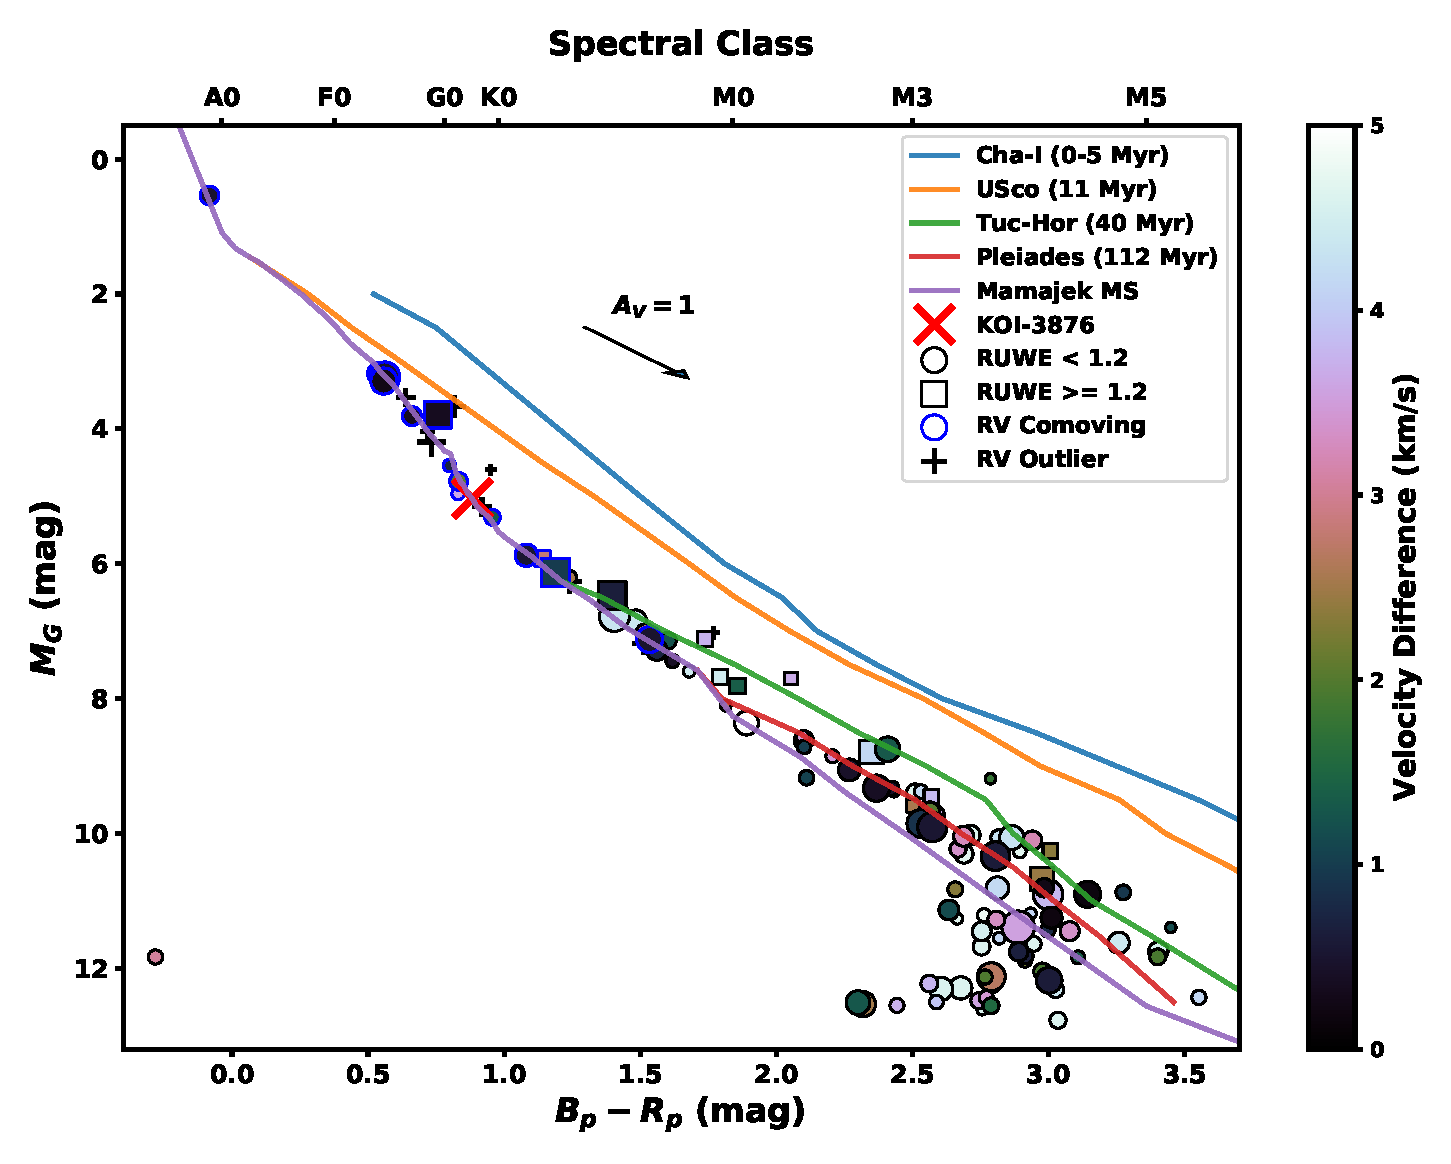
\includegraphics[width=0.48\textwidth]{KOI-3876_25cmd.pdf}
    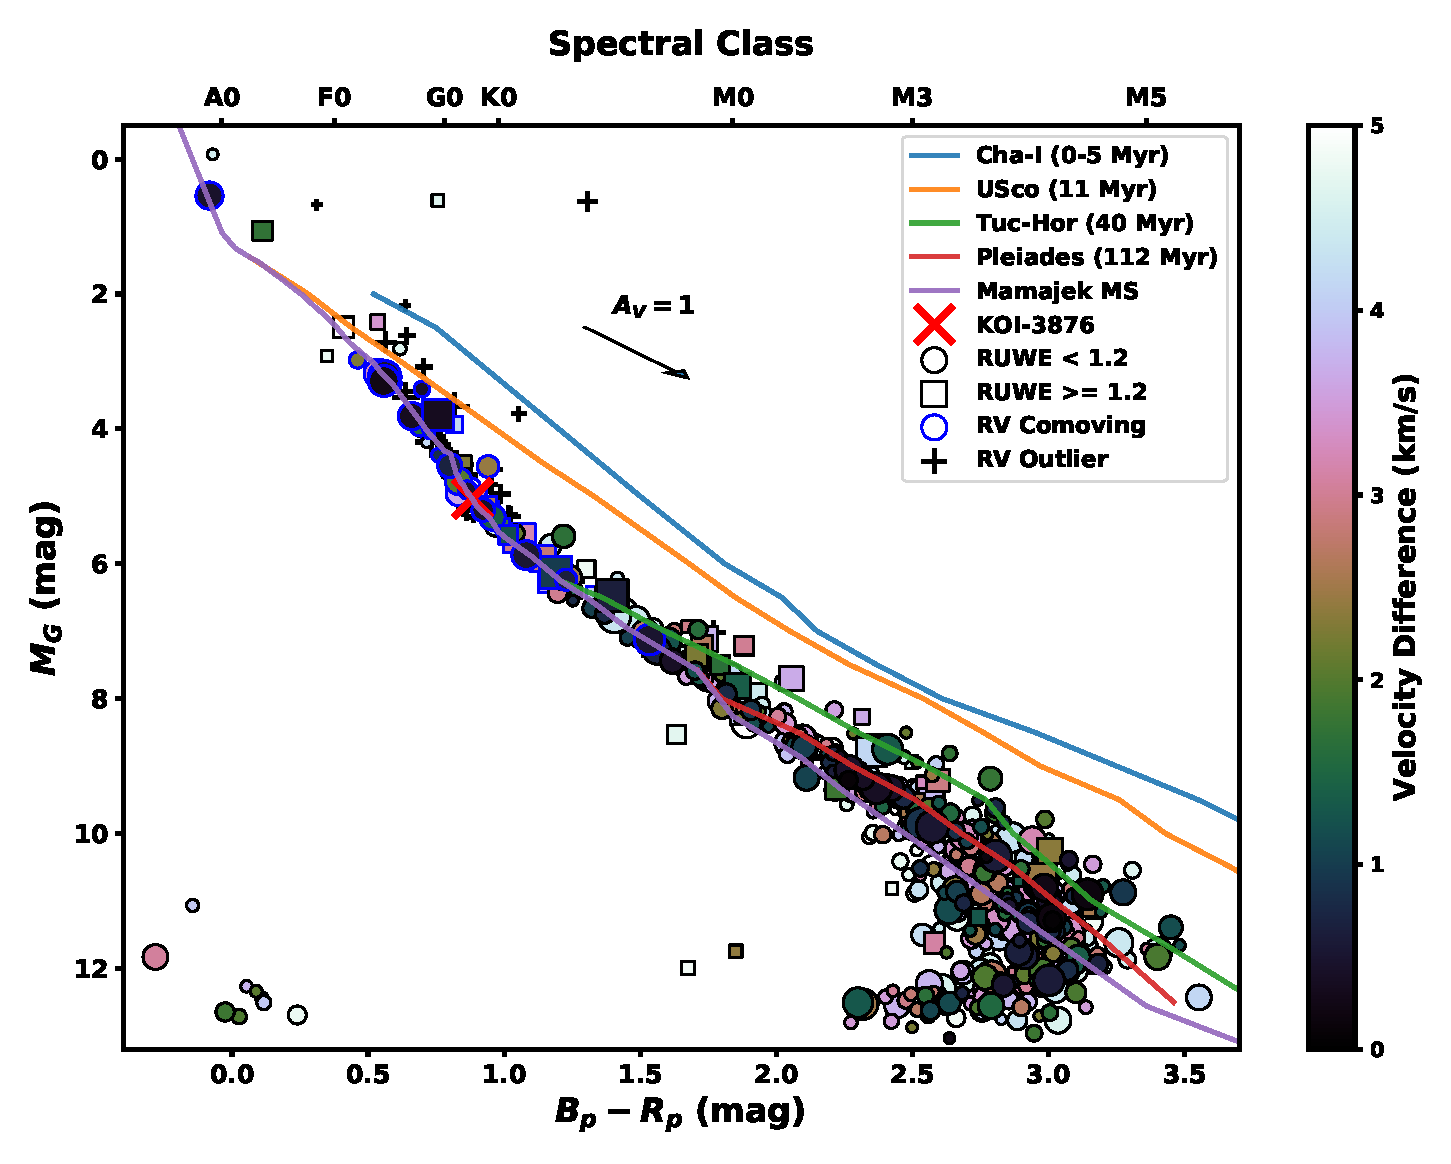
\includegraphics[width=0.48\textwidth]{KOI-3876_50cmd.pdf}
    \caption{\gaia\ color-magnitude diagram of all stars within 5\,\kms\ in tangential velocity and 25\,pc (left) or 50\,pc (right) of \starname. Approximate spectral types are shown on the top axis. Points are color-coded by the difference between their expected and observed tangential velocity assuming a perfect $UVW$ match to \starname\ and scaled in size by their distance from \starname. Points with radial velocities consistent with \starname\ are marked with blue circles and those with discrepant velocities are changed to a plus signs (and excluded from the color coding). Approximate single-star sequences from major nearby groups with known ages are shown as colored lines. These have not been corrected for reddening and are only used as a rough guide to the expected sequence.  }
    \label{fig:CMD}
\end{figure*} 

\begin{figure*}[tb]
    \centering
    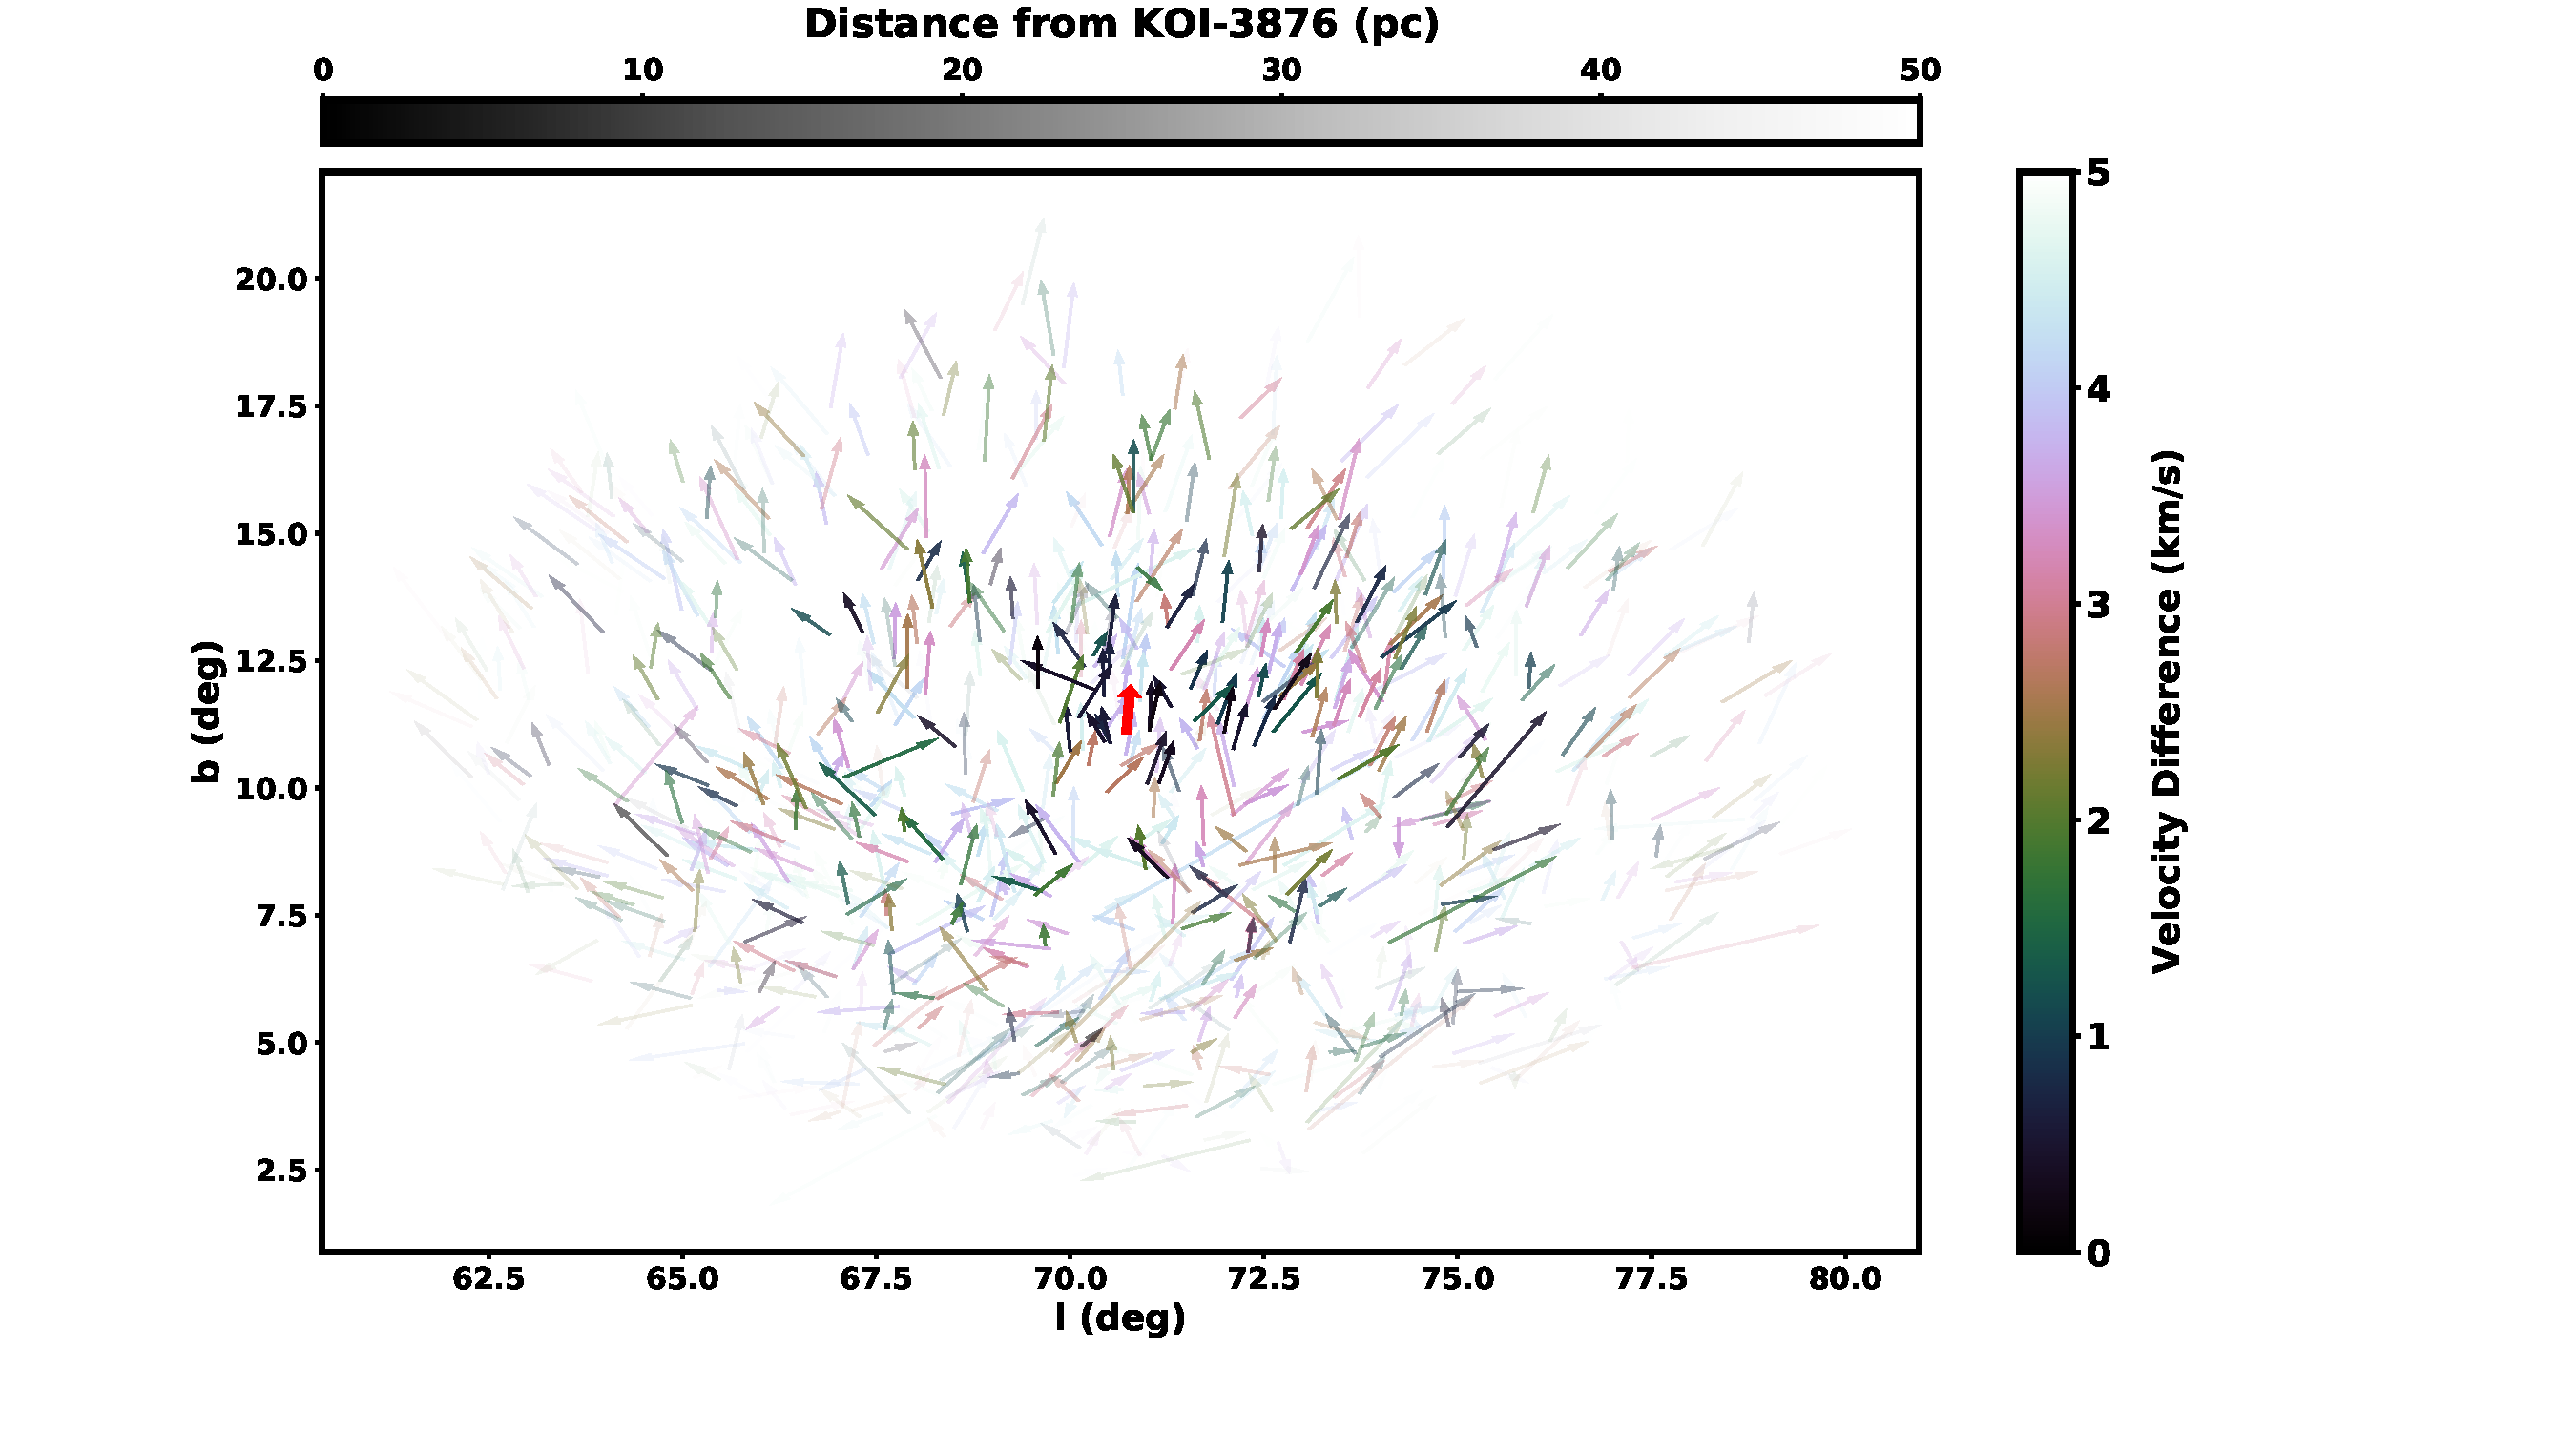
\includegraphics[trim=90 0 150 0,clip=true,width=0.98\textwidth]{propMotionFadedV3.pdf}
    \caption{Galactic coordinates and motions for all 1007 candidate members of \association. The red arrow shows \starname, and other stars are color-coded by their tangential velocity offset from \starname\ with transparency set by their physical distance from \starname. Arrows indicate the direction and (relative) magnitude of the proper motion. 
    }
    \label{fig:ProperMotion}
\end{figure*}

\section{Observations}\label{sec:obs}

\subsection{Optical spectra from McDonald 2.7 m \coude}\label{sec:tull}

We observed \name\ and 21 association candidates (Section \ref{sec:target}) with the \coude\ spectrograph on the Harlan J. Smith 2.7m telescope at the McDonald Observatory. The Robert G. Tull \coude\ is a cross-dispersed echelle spectrograph, delivering a R$\sim$60,000 spectral resolution from 3400--10000 \AA\  using the 1$\farcs$2 slit \citep{Tull1995}. Observations we're taken over the course of two observing runs, on 2021 July 9 and 2021 August 26--27. The sample was selected to include association candidates that could be observed with the \coude\ in modest exposure times ($G<13$), and spectral types later than mid-F ($B_p-R_P > 0.55$), where we expect lithium absorption to be a sensitive age diagnostic. The spectra are reduced with a custom python implementation of the standard IRAF procedures. Wavelength calibration made use of ThAr lamp spectra taken at the beginning, middle, and end of each night. the signal-to-noise of our spectra ranged between 14 and 60 per resolution element. 

To assess whether association candidates are co-moving in three dimensions, we measure radial velocities using spectral-line broadening functions (BFs). The BF is a linear inversion of an observed spectrum with a narrow-lined template, and represents the average stellar absorption-line profile. This profile (the BF) can be fit with a rotationally-broadened line profile to measure the stellar radial velocity and \vsini. We compute BFs for 34 spectral orders between 4300 and 9800 \AA that are free of telluric contamination using the {\tt saphires} python package \citep{Tofflemireetal2019}. BFs from individual orders are combined in to a single, high SNR BF and fit with a rotationally broadened profile \citep{Gray1992}. Narrow-lined templates, specific to each star, are taken from the \citet{2013A&A...553A...6H} PHOENIX model suite at the \teff\ closest to that provided by the \tess\ Input Catalog \citep[v8.0;][]{TIC2019}. Radial-velocity errors depend on the S/N and rotational broadening, but are generally on the order of 0.1 \kms. Measurements from the \coude\ spectra are provided in Table \ref{tab:sample}.

\subsection{Kepler and TESS light curves}\label{sec:lc}

\subsubsection{Light curves for transit search and characterization}
%\starname\ and \starnametwo\ were both observed by \kepler for the full 4.5 years at 30\,minute cadence. 
We searched for \kepler\ photometry for all 1007 candidates within the Mikulski Archive for Space Telescopes (MAST). A total of 84 targets had \kepler\ data, the majority of which had data from all quarters (Q0-Q17). We restricted our analysis to long-cadence data (30\,m), as short-cadence was not available for any of the planet hosts. For those lacking \kepler\ data, we instead downloaded \tess\ photometry wherever it was available through MAST. This included 15 targets with 2-minute cadence data, and 41 targets with 30-minute cadence data from the Quick-Look Pipeline \citep[QLP;][]{2020RNAAS...4..204H}. 

% This included all Quarters (Q0-Q17), providing more than 4 years of long-cadence (30\,m) photometry. 


% \starname\ was also observed by \tess\ at 120\,second cadence during Sectors 40 and 41. However, the \tess\ light curve was insufficiently precise to unambiguously recover the planet in the \tess\ data, so we did not use it for our analysis. 

% To search for any additional planets in \association, we obtained \kepler\ photometry for any candidate member with a light curve, a total of 84 targets. F

Where possible, we used the Pre-search Data Conditioning Simple Aperture Photometry \citep[PDCSAP;][]{Smith2012, Stumpe2012}. This included \starname, all \kepler\ candidate members, and the 15 targets with 2-minute cadence from \tess. For the remaining, we used the Quick-Look Pipeline light curves (Huang et al, 2020; https://arxiv.org/abs/2011.06459) for our planet search. Table~\ref{tab:sample} lists which stars have \kepler\ and/or \tess\ photometry that was used for our planet search. More details on our transit search can be found in Section~\ref{sec:search}.

The remaining 885 sources had no pre-extracted \tess\ or \kepler\ light curves. We did not extract additional curves from the full-frame \tess\ images for our planet search or characterization. The association association is more than 300\,pc away; most of the remaining stars were too faint to extract a light curve precise enough for our planet search. However, many such systems are still useful for measuring rotation periods.


\subsubsection{Light curves and literature search for rotation}\label{sub:rot_collection}

To assess membership and age of \association members, we collect stellar rotation periods using literature measurements supplemented by our own measurements from \kepler\ and \tess\ light curves. First, candidate members were cross matched against \citet{Nielsen:2013}, \citet{McQuillan2013, 2014ApJS..211...24M}, and \citet{Santos2019, Santos2021} for literature rotation periods. We matched candidate members to catalog members by \kepler\ Input Catalog (KIC) identifiers, which are listed in each catalog. We identified $56$ candidate members with available literature rotations, all but five of which have rotation measurements in multiple catalogs. For candidates that appear in only one catalog, we adopt the single measurement value. In cases where a star had measurements from more than one source, we adopt the average of the measurements as the rotation period. Only one object, KIC 3743810, had a conflicting rotation periods between catalog sources. Based on a visual examination of this object's \kepler\ PDCSAP light curve we selected the value from \citet{Nielsen:2013}.

For stars without literature rotation periods we performed our own analysis. Priority was given to \kepler\ PDCSAP data followed by \tess\ full-frame images. To generate the \tess\ light curves for rotation analysis, we first created raw flux light curves from the FFI cutouts centered on each candidate. Then, we generated a Causal Pixel Model (CPM) of the telescope systematics using the \texttt{unpopular} package \citep{2021arXiv210615063H} for each individual star. We subtracted the CPM systematics from the initial light curves, resulting in the light curves used for our rotation search described in Section~\ref{sec:rotation}.

\subsection{Archival photometry and astrometry}
We download positions, parallaxes, proper motions, and $B_P$, $R_P$ and $G$ photometry for all candidate members of \association\ using the third \gaia\ Early Data Release \citep[EDR3;][]{GaiaEDR3}. For \starname, we also retrieved photometry from the Two-Micron All-Sky Survey \citep[2MASS;][]{Skrutskie2006}, the Wide-field Infrared Survey Explorer \citep[WISE; ][]{allwise}, and the AAVSO All-Sky Photometric Survey \citep[APASS; ][]{apass}. Photometry for \starname\ is listed in Table~\ref{tab:prop}. 


\subsection{Archival Velocities}
In order of preference, we drew radial velocities for candidate \association\ members from the second \gaia\ data release \citep[DR2;][]{DR2_velocities}, the sixteenth APOGEE data release \citep[DR16; ][]{2020AJ....160..120J}, and the fifth LAMOST data release \cite[DR5; ][]{2015RAA....15.1095L, 2019yCat.5164....0L}. Velocities from our own spectra (Section~\ref{sec:tull}) were given the highest priority. In the instance where a star had multiple velocities from the same star we used the weighted mean and error. We did not combine multiple velocities from different sources due to possible differences in the zero-points. 

%\textcolor{orange}{I clearly applied a velocity offset of about 5 km/s to LAMOST to match APOGEE. I need a reference for this and I need to document it. }

In total, we adopted \gaia\ RVs for 56 stars, APOGEE RVs for 5 stars, and LAMOST RVs for 25 stars. This was in addition to velocities from our Coude spectra for 22 candidate member stars as well as \starname. We applied an offset to the LAMOST velocities of +4.54\kms\ based on the comparison from \citet{2018A&A...620A..76A}. There may be additional zero-point differences between the velocity sources, but these are likely larger than the internal velocity spread within the group. The adopted velocities are given in Table~\ref{tab:sample}.




\section{Search for planets in MELANGE-2}\label{sec:search}

\textcolor{red}{did you use notch and locor, or just notch?}
To check for other candidate planets or eclipsing binaries in the same association we searched the \textcolor{red}{265} \kepler\ and \tess\ light curves using the Notch pipeline pipelines. The details of both pipelines are described in more detail in \citet{Rizzuto2017}. To briefly summarize, the Notch filter fits a window of the lightcurve as a combination of an outlier-robust second-order polynomial (for the stellar variability) and a trapezoidal notch (representing the potential planet). The window moves along the lightcurve until the variability is detrended while preserving the planet signal. At each data point, we calculate the improvement from adding the trapezoidal notch based on the change in the in Bayesian Information Criterion (BIC) compared to modelling just a polynomial. LOCoR (Locally Optimized Combination of Rotations), instead models the stellar variability using linear combinations of pseudo-rotation measurements in other parts of the light curve than the region being modeled. It then repeats this process over the full curve. 

We searched the detrended light curves (both Notch and LOCoR detrended) and the BIC signals that Notch produces for periodic signals. We excluded the rotation period (and aliases) of the star, as it is common to have imperfect detrending with both algorithms. In addition to our search, a number of known \kepler\ objects of interest (KOIs) reside within candidate members of \association, identified by a simple cross-match against the most recent KOI catalog \citep{2016AJ....152..158T}. 

In total, we identified 18 targets of interest that are either KOIs and/or pass the SNR and initial quality checks from Notch/LOCor. Eight of these are known KOIs (KOI-678.01, KOI-678.02, KOI-966.01, KOI-966.02, KOI-1838.01, KOI-5304.01, KOI-6819.01, and KOI-7059.01), while the remaining are newly identified. 

All 18 targets are listed in Table~\ref{tab:kois-kics} along with our classification of each. Other than \planetname, we concluded only one other detection (Kepler-970\,b) was both a real planet and a member of \association. We discuss each system and our reasons for rejection them below.



% explain notch
% Notch attempts to fit a polynomial with a trapezoid (the "notch") to every point on the light curve. Notch detrends the light curve by flattening the polynomial that is used to model sections of the light curve. A Bayesian Information Criterion (BIC) value is assigned to every data point based on how well the notch models that point versus modeling the data point with just a polynomial without the trapezoidal cut out. The BIC takes into account the number of data points, the number of fit parameters, and the likelihood function of the model. The probability factor that we obtain is a measure of how well the model fits the data. These BIC values are normalized on a scale between 0 and 1, with 0 meaning the data point is very likely to be the center of a signal and 1 meaning there is likely no signal present at the data point. 

% explain locor

% explain bls search
% The Box Least Squares (BLS) search in the Notch and LOCoR package uses the detrended light curve after running either Notch or LOCoR on the light curve. The function runs an iterative BLS search on either the detrended light curve or the BIC sequence of the light curve. It searches for transits by looking for regular small BIC values. If a planet is identified, it will be removed from the detrended light curve or BIC model before the algorithm looks for an additional planet. 

% what we did
% We executed bulk searches of various stars in TESS data and Kepler data using Notch and LOCoR to look for promising targets. The THYME Team collaboration provided an initial list of known young stars from ESA’s Gaia mission. Using the lightkurve python package //cite//, we obtained the light curve for each target and ran it through the Notch and LOCoR pipeline. We were able to identify the KOI3876 transit, as well as a number of other eclipsing binaries, KOIs, TOIs, and false positives in the association.
% talk about the initial FP disposition here? or in FP analysis?

%We flagged X interesting things. Y of them were previously-noted KOIs (KOI X, KOI Y, KOI Z). Z of them were new. We concluded that KOI A was an EB (Figure). KOI 1234, 5678, were interesting, but low SNR, so we just consider these candidates. We summarize it all in Table~\ref{tab:tablename}.
%Interesting objects: 9 T/KICs + 8 KOIs, stars: 6 KOI + 6 T/KICs

\subsection{Discussion of individual candidates}

KOI-1838.01 is a confirmed planet \citep[Kepler-970 b;][]{2016ApJ...822...86M}. The star's rotation (9.3\,days) places it right on the Pleiades sequence, and much faster than the stalling regime seen for $>600$\,Myr systems \citep{Curtis_stall}. The LAMOST (corrected) velocity is -32$\pm$4\,\kms, which is consistent with the value predicted for membership ($\simeq$-27\kms). A more precise measurement from the CKS-cool project (Petigura et al. 2021) yielded an RV of -27.15$\pm$0.10\kms, a nearly perfect match for the association. The spectra shows weak lithium ($<50m\AA$), but this is consistent with 100\,Myr for its spectral type \textcolor{red}{CITE A MODEL}. As we show in Figure~\ref{fig:CMD}, Figure~\ref{fig:ProperMotion}, and Figure~\ref{fig:xyz}, \starnametwo\ is consistent with \association's color-magnitude diagram, proper motion, and Galactic position. \textcolor{red}{ALL THREE PLOTS SHOULD BE UPDATED}. We conclude that this planet is real and a member and include it in our analysis of \starname.

%\textcolor{red}{Calculate UVW XYZ for this target. Add to plots? Comment on position within the cluster. Comment on conclusion and future follow-up. The Li levels look like <30mA; but this is in a region where it could be depleted. Unclear. The HIRES data also suggests RV = -30. I think this is a member, but the current evidence is thin. We should ask the HIRES people? We need to rewrite some of the paper if there's two planets.  }

KOI-678 (.01 and .02) contains two confirmed planets (Kepler-211\,bc), and the star's light curve showed a clear rotation signature of $\simeq$13.7\,days. However, this period is too long for membership given its \gaia\ colors (should be $\lesssim$8\,days). Similarly, the lithium equivalent width is only 3.8$m\AA$ \citep{2018ApJ...855..115B}, but membership would suggest a Li level above 100$m\AA$. The star's proper motion also puts it on the outskirts of the distribution. We conclude this target is unlikely to be a member. 

Both planet candidates in KOI-966 are flagged as false positives by the \kepler\ analysis \citep{2016ApJS..224...12C}, with both signals attributed to an eclipsing binary (.02 corresponding to an alias of the secondary eclipse). We similarly concluded that the signal is likely an eclipsing binary based on the V-shaped transit and secondary eclipse. The star's rotation period \citep[3.92\,days;][]{2013MNRAS.436.1883W} is consistent with membership for an M dwarf and does not match the eclipse period (0.379\,days). The star is also only 1\kms\ and 8\,pc from \starname, near the core of likely members. We conclude it is likely an eclipsing binary in the association.

% KOI-1838.01

% 2101379205604338688 & 289.62522 & 40.70874 & 14.788 & 3.102 & K5.3 & N & Y & 3.015 & 0.019 & 9.23 & 0.66 & 3 & $\ldots$ & $\ldots$ & -36.534 & 3.723 & 6 \\


% While the star's rotational period $\simeq$9.3\,days is as expected for its \gaia\ colors, the tangential velocity is $\gtrsim$3\kms\ from that of \starname. Additionally, the radial velocity of KOI-1838 is -36\kms\ //from LAMOST//, which is about 10\kms\ off from \starname. We conclude this target is unlikely to be a member.\textcolor{red}{Uh, wait a sec, LAMOST RVs suck. The real rv is -31, it should be -36, and the error is 4. So it's consistent. It has no significant Li, but at bp-rp = 1.5, it should be Li depleted. This might be a legit member!}

% KOI-6819.01 
KOI-6819 contains a planet candidate (.01). The star shows no significant rotation, suggesting the star is of older age. We find KOI-6819 has a radial velocity of 3.27\kms\ //gaia dr2//, $>$20\kms\ off from \starname. KOI-6819 shows no Li signature, when we would expect $>$50$m\AA$. We conclude this target is unlikely to be a member. 

% KOI-7059.01
KOI-7059.01 is flagged as a false positive by the \kepler\ analysis \citep{2016ApJS..224...12C}, and the odd-even depth difference strongly suggests and eclipsing binary. KOI-7059 is $>$48\,pc from \starname. We conclude this target is likely a real eclipsing binary but unlikely to be a member.

% KICs 1137886, 6134939, 6366739, 6589221, 9139566, and 9700914 and TICs 164461070, 20352534, 272486188, 273383615, 28768382, and 355909811
For the newly identified targets, KICs 1137886, 6134939, 6366739, 6589221, 9139566, and 9700914 and TICs 164461070, 20352534, 272486188, 273383615, 28768382, and 355909811, we ultimately find that the SNR is below what we required for significance. This was determined by the BIC score for each target, where we found the BIC was below our threshold of significance for all targets. Even targets with the most transit-like signal (U-shaped and of reasonable depth), such as KIC 6589221 shown in Figure \ref{fig:kic221transit} and KIC 9700914 shown in Figure \ref{fig:kic914transit}, were deemed simply likely candidates. 

% argue candidacy of each -- can lump together similar cases
TICs 28768382 and 272486188 and KICs 9139566 and 9700914 are unlikely to be members due to the $>$20\kms\ difference in expected versus actual radial velocity. % add measured rvs and sources

KIC 6589221, while is 42pc from \starname, we find to be within 2.2\kms\ of \starname\ and have a radial velocity of -24.44\kms\, which is $<$2\kms\ from expected. The stellar rotation of $\simeq$5.4 days closely matches the expected rotation period for its \gaia\ color. Further, the star's proper motion closely matches \starname. We conclude this target is likely to be a member.


KOI-1838.01, KOI-678.01, and KOI-678.02 are confirmed planets, while KOI-6819.01 is still considered a planetary candidate. Using existing spectra from Exofop (//cite//), radial velocities from Gaia (//cite//), and rotational periods and activity metrics where available, we conclude all KOIs except KOI-966 are likely not members of the association. Based on it's rotational period, KOI-966, a clear eclipsing binary, is still likely a member. Notch and LOCoR flagged KICs 1137886, 6134939, 6366739, 6589221, 9139566, and 9700914 and TICs 164461070, 20352534, 272486188, 273383615, 28768382, and 355909811 as interesting targets possibly containing one or more transiting bodies. Due to the low SNR, we just consider these candidates. We summarize all findings in Table \ref{tab:kois-kics}.


%we rejected KOI612 (TICXXX) because the Li equivalent width from Berger et al (XXX) was only 3.8mA, while we expect levels to be >100mA at this age and spectral type. Similarly, while the star shows clear rotation, the rotation period (13.X days, citation) is well above the Pleiades sequence

\begin{deluxetable}{lccc}
\centering
\tabletypesize{\scriptsize}
\tablecaption{Planetary Candidates in \association. \label{tab:kois-kics}}
\tablehead{\colhead{ID} & \colhead{Disposition} & \colhead{Probable Member?} }
\startdata
\hline
KOI-678.01 & Confirmed & N \\
KOI-678.02 & Confirmed & N \\
KOI-966.01 & EB & Y \\
KOI-966.02 & EB & Y \\
KOI-1838.01 & Confirmed & N \\
KOI-5304.01 & FP & N \\
KOI-6819.01 & Candidate & N \\
KOI-7059.01 & EB & N \\
\hline
KIC 1137886 & Candidate & \\
KIC 6134939 & Candidate & \\
KIC 6366739 & Candidate & \\
KIC 6589221 & Candidate & Y \\
KIC 9139566 & Candidate & N \\
KIC 9700914 & Candidate & N \\
TIC 164461070 & Candidate & \\
TIC 20352534 & Candidate & \\
TIC 272486188 & Candidate & N \\
TIC 273383615 & Candidate & \\
TIC 28768382 & Candidate & N \\
TIC 355909811 & Candidate & \\
\enddata
\end{deluxetable}

\begin{figure}[tb]
    \centering
    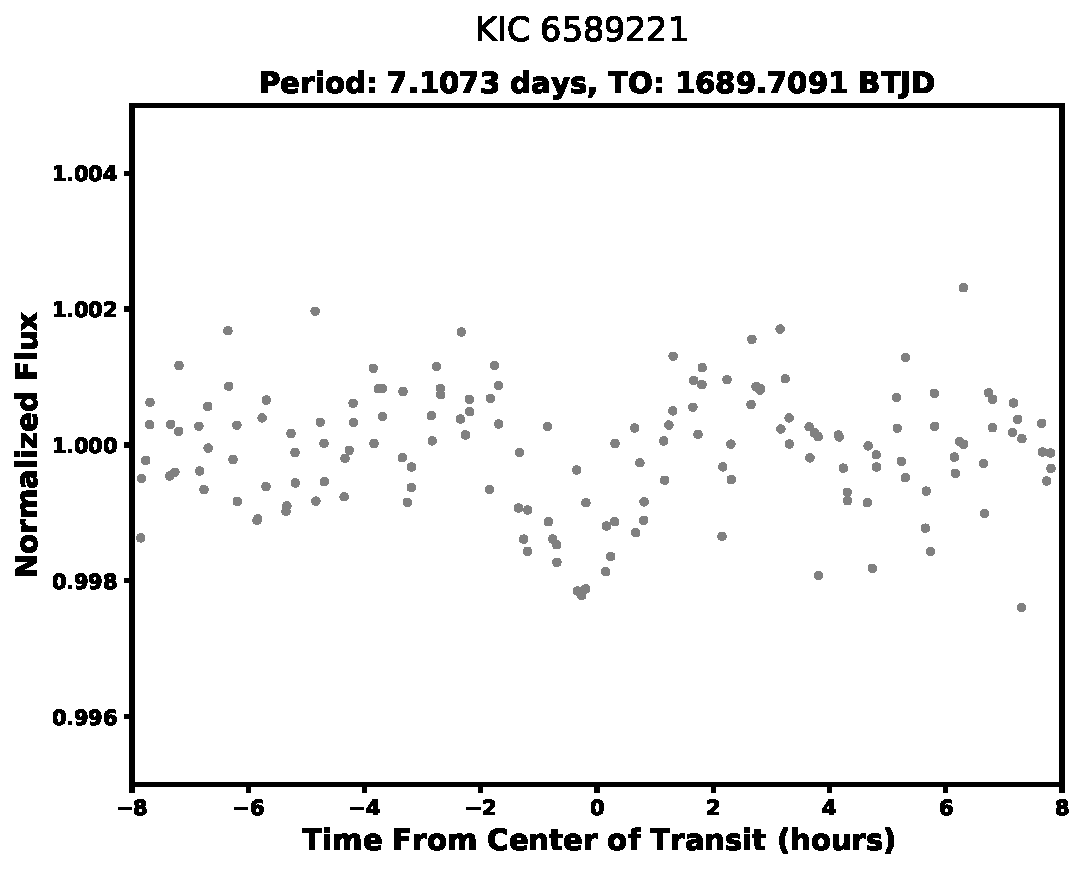
\includegraphics[width=0.49\textwidth]{KIC6589221LC.pdf}
    \caption{Phase-folded light curve of potential member KIC 6589221 from \tess\ detrended with Notch and LOCoR (grey points). We find that the bestfit period is 7.1073 days, with an initial transit time of 1689.709 BTJD. }
    \label{fig:kic221transit}
\end{figure}

\begin{figure}[tb]
    \centering
    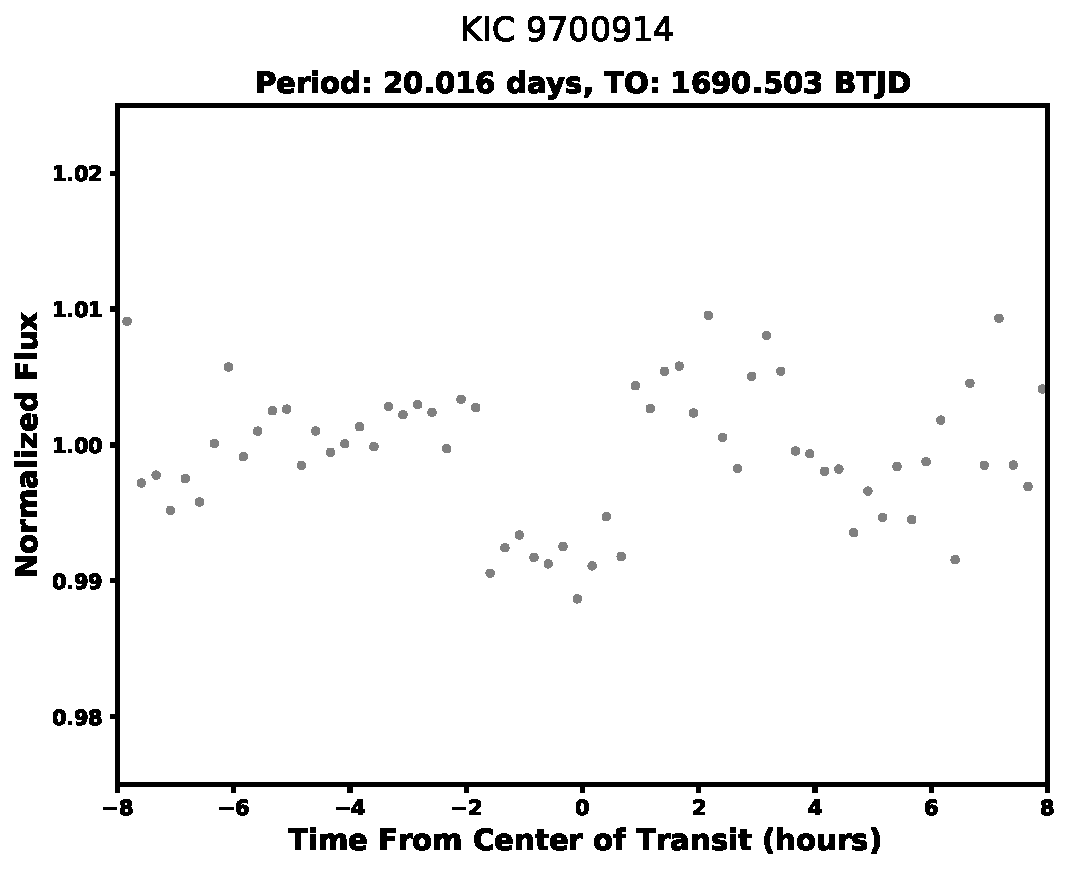
\includegraphics[width=0.49\textwidth]{KIC9700914LC.pdf}
    \caption{Phase-folded light curve of potential member KIC 9700914 from \tess\ detrended with Notch and LOCoR (grey points). We find that the bestfit period is 20.016 days, with an initial transit time of 1690.503 BTJD. }
    \label{fig:kic914transit}
\end{figure}



\section{The MELANGE-2 Association}\label{sec:cluster}

\subsection{Position and Kinematics}


\textcolor{red}{AWM: note to self, this needs some editing. }

For each of the 1007 candidate members of MELANGE-2, we show show the Galactic $XYZ$ position in Figure~\ref{fig:xyz} and the proper motion in Galactic coordinates ($l$, $b$) in Figure~\ref{fig:ProperMotion}. Since our initial search used a generous search of 50\,pc and 5\kms\ (tangential) from \starname, 

We originally identified a group of 998 stars within 50pc and 5 km/s of \starname using //friendfinder//. 

As can be seen in Figure \ref{fig:xyz}, most //give percentage// targets in the field have velocities greater than 4 km/s of \starname, shown in pink. These are likely non-member background stars. However, we can see a cluster of high probability members that are within 1 km/s of \starname, shown in black. We can see that these targets are tightly packed in z, between 58pc and 75pc, as expected based on the argument by //z argument paper//. In x and y, we see a streak as expected due to the rotation of the galaxy and the spreading of the cluster over time.

In Figure \ref{fig:ProperMotion}, we see a tight cluster of co-moving stars, shown in black surrounding \starname, shown in red. We again see a large proportion of likely background stars moving separately from the core group.


\begin{figure*}[tb]
    \centering
    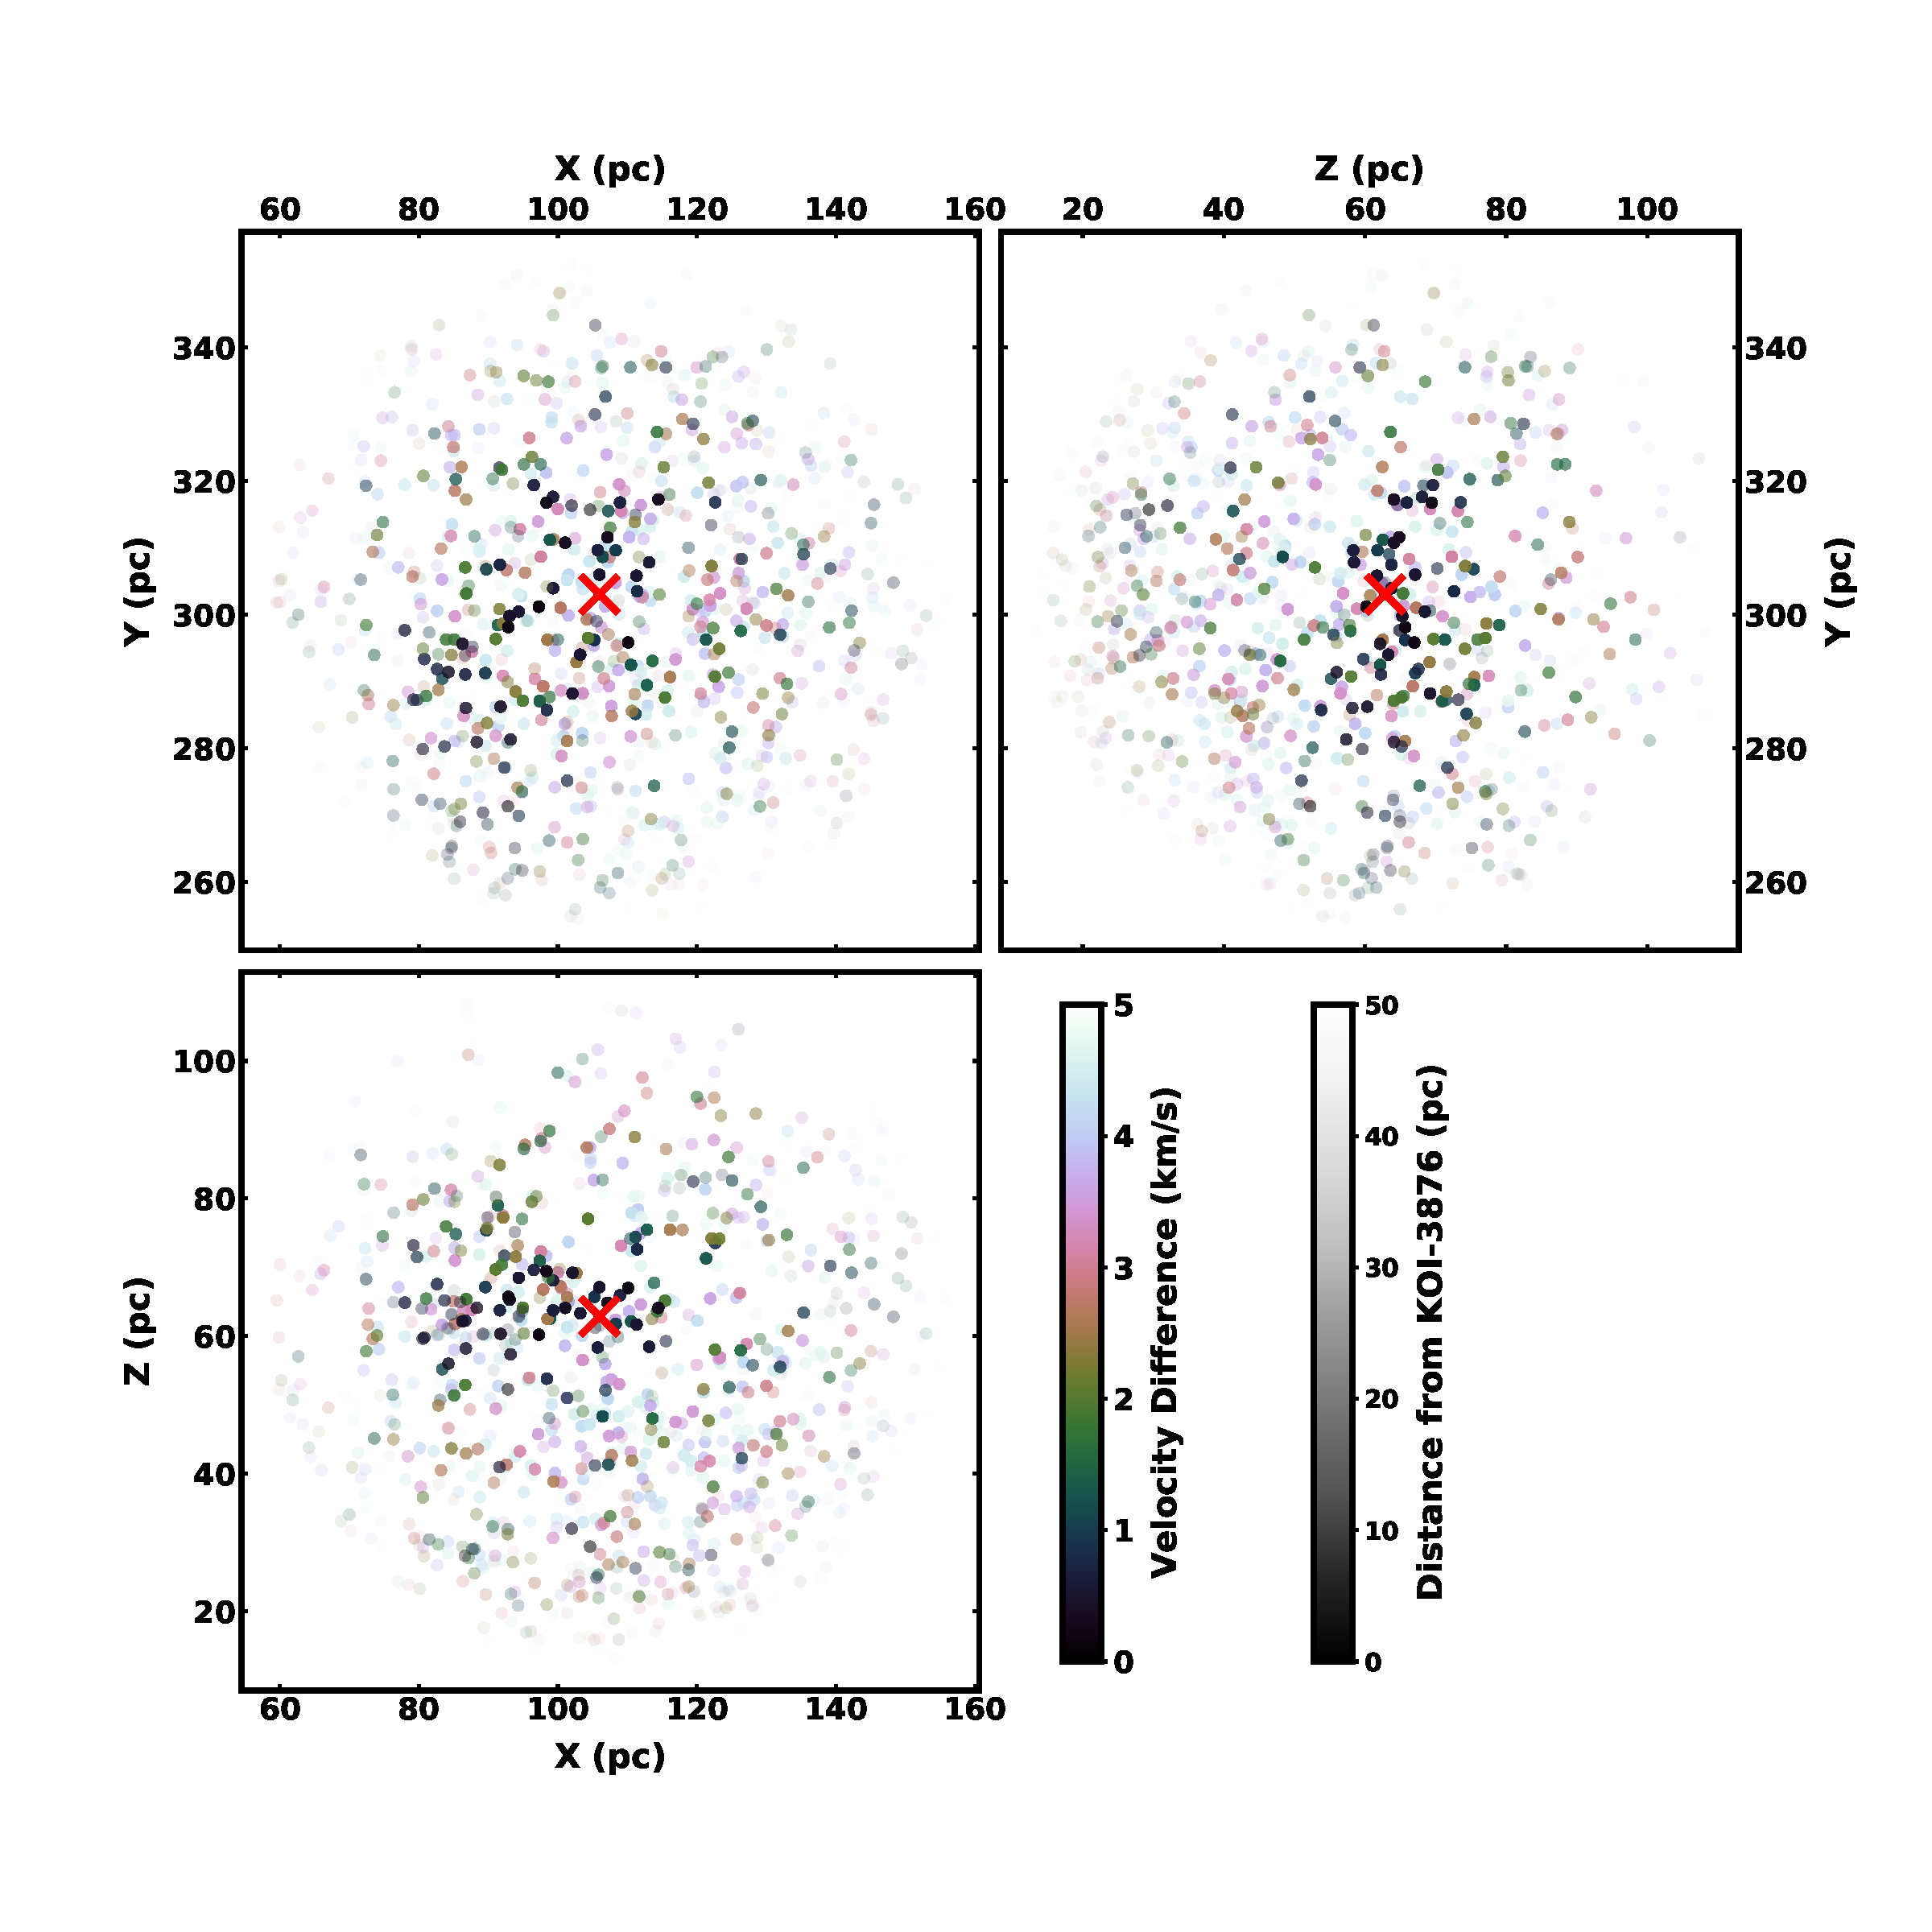
\includegraphics[width=0.98\textwidth]{xyzSpaceFadedV2.pdf}
    \caption{\textcolor{red}{needs a caption here.} Galactic Heliocentric (XYZ) coordinates of stars within 50pc and 5km/s of \starname (marked as a red X). Color indicates the velocity difference from \starname, and the transparency indicates distance from \starname.}
    \label{fig:xyz}
\end{figure*} 
    
\subsection{Isochronal age}

We estimated the age of \association\ by comparing the CMD to the PARSEC (v1.2S) models \citep{PARSEC}. We used a mixture model, as detailed in Mann et al. (in prep)\footnote{\url{https://github.com/awmann/mixtureages}}, based on the method outlined in \citet{HoggRecipes}, and wrapped in a Monte-Carlo Markov-Chain using \texttt{emcee} \citep{Foreman-Mackey2013}. To briefly summarize, we fit the population with the combination of two models. The first described the single-star member sequence drawn from PARSEC models. The second is an outlier population, which may itself contain a mix of populations (e.g., binaries, field interlopers, and stars with erroneous parallaxes or photometry). The fit included six free parameters: the association age (age), the average reddening across the association ($E(B-V)$), the amplitude of the outlier population ($P_B$), the offset of the outlier population from the main population CMD ($Y_B$ [mags]), the variance of the outliers around the mean ($V_B$ [mags]), and a term to capture missing uncertainties or differential reddening across the association ($f$ [mags]). 

Reddening was limited to $<0.2$ mag based on the three-dimensional extinction map from \citet{2019ApJ...887...93G}. Other parameters evolved under uniform priors, bounded only by physical limits. We re-sampled the model grid to ensure uniform distribution around the expected age (50-250\,Myr). 

\gaia\ photometry was the only available for all targets, and was generally far more precise than other data available. Many stars were also resolved as binaries (or the target and a background star) in \gaia, but seen as a single source in 2MASS and KIC photometry \citep{Brown2011}. So we restricted our analysis to \gaia\ magnitudes. 

We expect most of the initial sample of 1007 candidate members to be field interlopers. While the mixture model can handle high contamination rates by making $P_B$ larger,  tests suggest the fit prefers call the true population of interest the outliers and instead fit the background population as the true one. To avoid this, we limited the input list to stars within 30\,pc and 3\kms\ from \starname\ in three-dimensional distance and tangential velocity. We also removed any stars with a Renormalised Unit Weight Error \citep[RUWE; ][]{GaiaEDR3} $>1.2$. As discussed in \citet{Ziegler2020} and \citet{2021arXiv210609040W}, stars above this limit are likely to be binaries. Lastly, we removed any stars that were outside the model grid range based on their absolute magnitude and/or color and stars with poor photometry or parallaxes (SNR$<$20). This left only 78 stars, but this was more than sufficient for a fit.% Loosening the tangential and separation cuts 

As we show in Figure~\ref{fig:isochrone}, the resulting fit yielded an age of 104$^{+8}_{-5}$\,Myr. As a test of the systematic errors, we ran a similar fit using models from the Dartmouth Stellar Evolution Program \citep[DSEP,][]{Dotter2008} with magnetic enhancement described in \citet{Feiden2012b}. The DSEP-magnetic model fit gave a similar age of 110$\pm$11\,Myr. The DSEP magnetic models did somewhat better for the low-mass stars, and yielded a more conservative uncertainty, so we adopted this as the isochronal age.

\begin{figure}[tb]
    \centering
    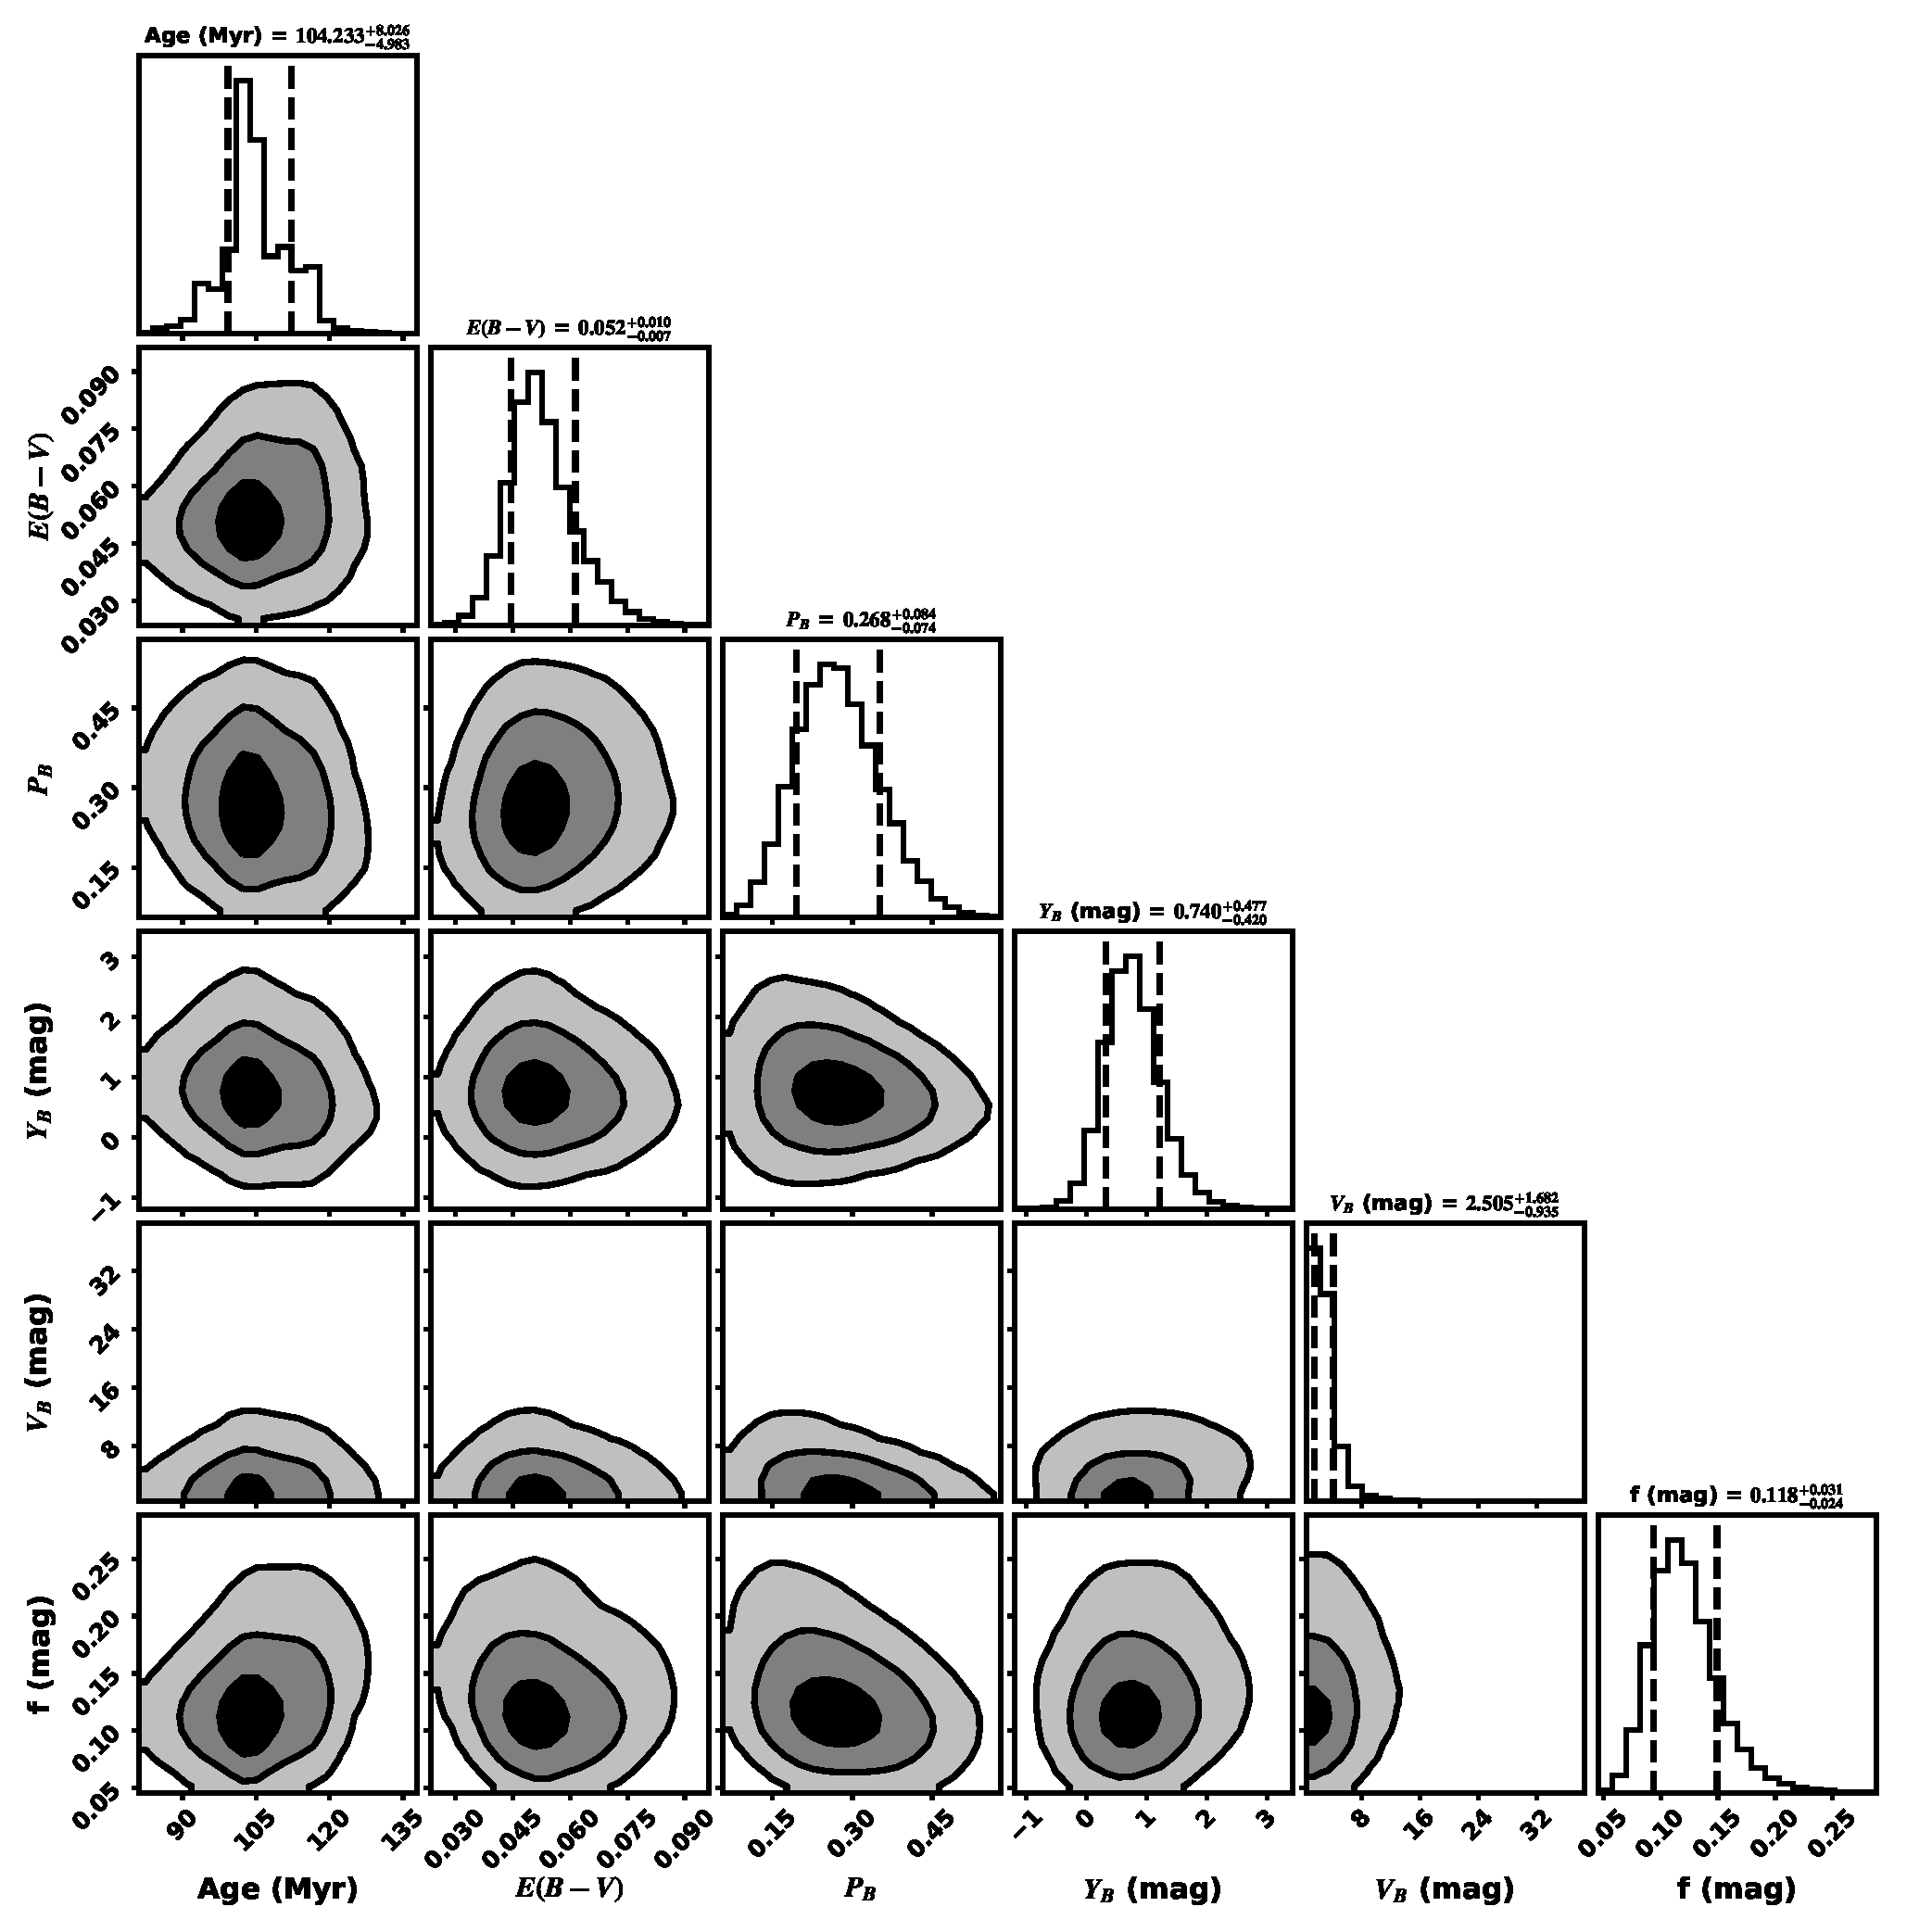
\includegraphics[width=0.49\textwidth]{cornerhybrid_parsec_bprp_g_edr3.pdf}
    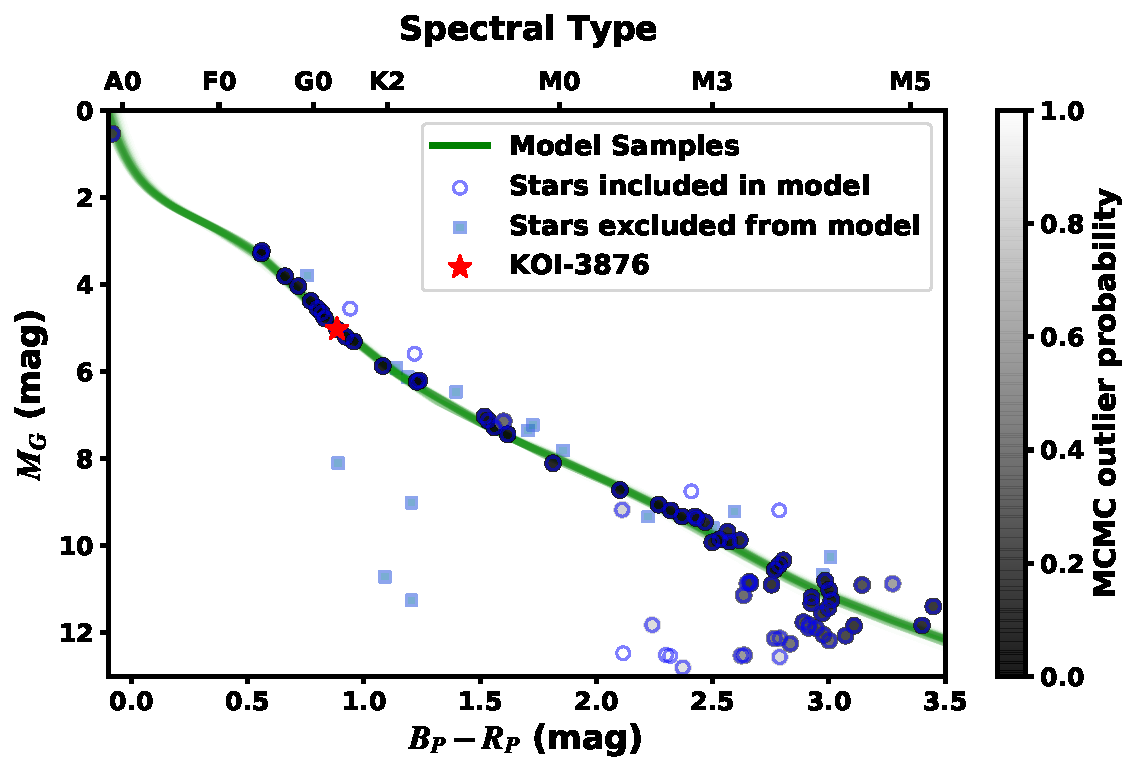
\includegraphics[width=0.49\textwidth]{CMDcoloroutlierhybrid_parsec_bprp_g_edr3.pdf}
    \caption{Comparison of the PARCSEC model isochrones to candidate members of \association. The top shows the corner plot of our MCMC mixture model comparison, with contours corresponding to $1\sigma$, $2\sigma$, and $3\sigma$. The bottom plot shows the \gaia\ $G$ versus $G-R_P$ CMD of stars included in the MCMC (blue circles) and those excluded (blue squares) due to their RUWE, color, or magnitude. Each included point is shaded based on their average outlier probability as determined by the MCMC. Many of those flagged as outliers may be non-members or members that do not follow the sequence (e.g., binaries). \starname\ is shown as a red star. The green lines are 200 PARSEC isochrones with parameters drawn (randomly) from the MCMC posterior.  }
    \label{fig:isochrone}
\end{figure} 



\subsection{Lithium}

%\textcolor{red}{Let's check this with Ben Tofflemire}
%We estimated Li EWs for each of the seven stars kinematically associated with HD 110082 using our Goodman spectra (Section 2.3.2). We simultaneously fit the width, depth, center, and the continuum line using a region around 6707.8 Å and assuming a Gaussian profile. The fit parameters were limited by physical and measurement constraints, e.g., the line center was allowed to deviate by 0.1 Å from 6707.8 Å (the error on our wavelength solution and rest-frame correction) and the width restricted by the spectral resolution and expected rotational broadening. The continuum was fit iteratively, rejecting points >3σ below the continuum fit to handle nearby absorption lines. We measured the final EW from the Gaussian fit to the region. These measurements include the contribution from the nearby iron line, Fe i 6707.4 Å. We consider EW measurements below 0.01 Å to be upper limits.


We measured the equivalent width of the Li 6708\,\AA\ line for 22 stars (including \name) using the Coude spectra described in Section~\ref{sec:tull}. Using our measured radial and rotation velocities from the BF analysis, we shifted each spectrum to zero velocity and compared it to a rotationally broadened template of the same \teff. We then interactively defined regions of continuum between 6685 and 6730 \AA, and the bounds of the EW integration. We measured the Li EW and its uncertainty using a bootstrap approach. The continuum was first fit using {\tt emcee}, 1000 random draws from the fit posterior are used to normalized the spectrum, and for each realization, the Li absorption line is numerically integration 10 times where the integration bounds are varied randomly from a normal distribution with the width of a resolution element. This procedure results in 10,000 Li EW measurements, we take the median and standard deviation as our final measurement and its uncertainty, respectively.  
%To account for variations in resolution, \vsini, and velocity between datasets, we first fit nearby atomic lines with a Gaussian profile (e.g., iron lines for warmer stars and K lines for the M dwarfs). We used the width from these fits to define the bounds of the Li line. To estimate the pseudo-continuum, we iteratively fit the 6990--6720\AA\ region excluding the Li line, each time removing regions $>$4$\sigma$ below the fit (there were no emission lines in this region). 

Past detections of Li with the same observational setup and our typical spectrum SNR indicate we were sensitive to Li down to equivalent widths of $20m\AA$ or better. So we report this as our upper limit when no line is detected. One star (Gaia EDR3 2052858307226740352) had a \vsini$>50$\kms, which made extraction of the Li line unreliable. So we instead reported a $<70m\AA$ upper limit for this source based on past detections on similarly broadened spectra. 



For \starname, we estimated a Li equivalent width if 134\,$m\AA$. This is marginally higher than (but consistent with) the value from \citet{2018ApJ...855..115B} (120\,$m\AA$). We attribute this difference to \citet{2018ApJ...855..115B}'s removal of the Fe line at 6707.44\,\AA. We did not attempt to correct for this contamination or from broad molecular contamination in the cooler stars. Fe line contamination likely set a limit on the precision of our equivalent widths at the $\simeq$10\% level, comparable to the measurement errors. The difference was small compared to the offset in Li levels between clusters; we used our Li measurements for all targets for consistency.

Two spectra (Gaia EDR3 2101333021814076800 and 2048317736525727488) had two clear sets of lines, indicating an SB2. For our Li measurements, we measured each line individually with a manually-applied velocity offset. We then combined the two equivalent widths. 

We compared the Li sequence for \association\ to that from the $\simeq$112\,Myr Pleiades \citet{2018A&A...613A..63B} and the 650-700\,Myr Hyades from \citep{2017AJ....153..128C} in Figure~\ref{fig:lithium}. The \association\ sequence is nearly identical to that from Pleiades. The Li sequences of nearby clusters from \texttt{BAFFLES} \citep{BAFFLES2020} suggested an age between 85\,Myr and 200\,Myr, consistent with our isochronal age. This age range is conservative, as the bounds can only be set using the set of clusters with ages and extant lithium sequence measurements. For the upper bound, this was set by M34 and M35 (200-300\,Myr).

\begin{figure}[tbh]
    \centering
    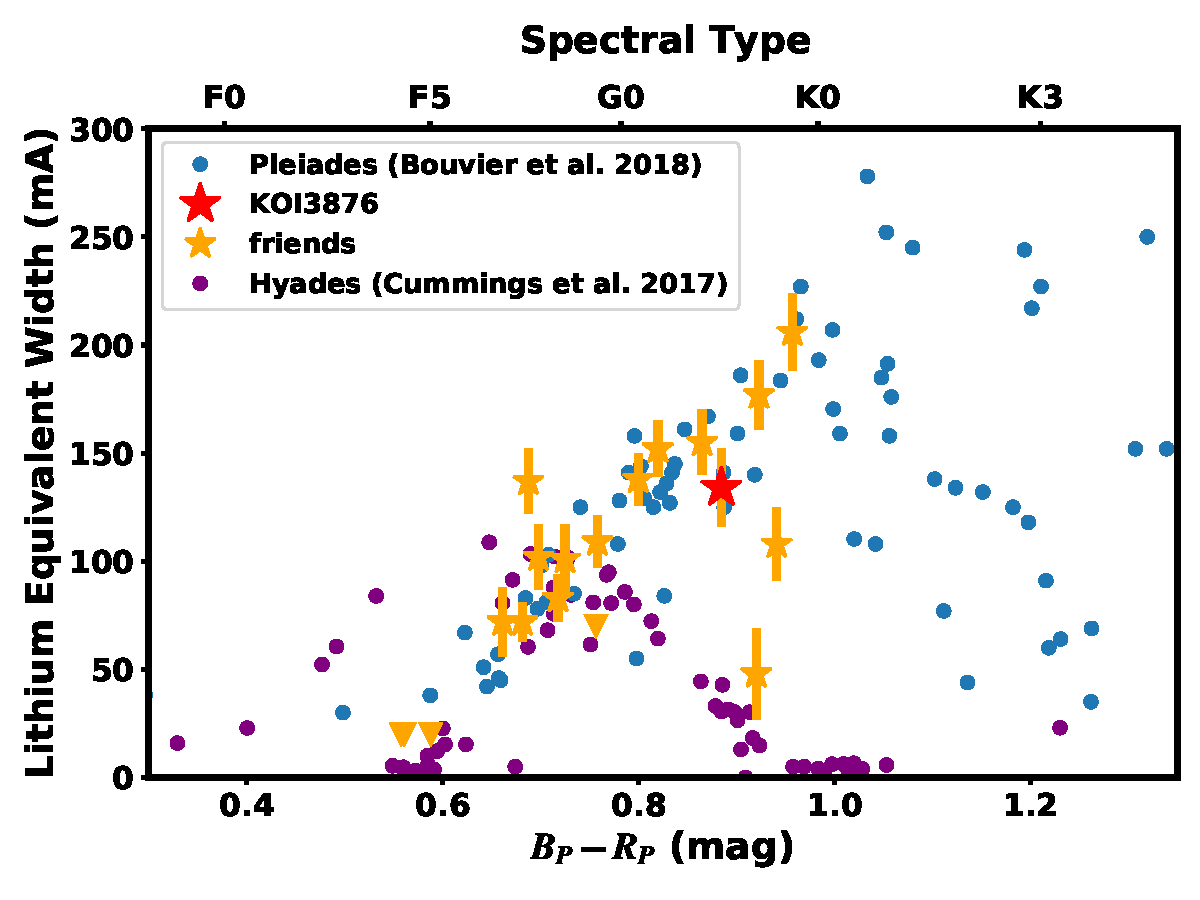
\includegraphics[width=0.47\textwidth]{lithium.pdf}
    \caption{Lithium equivalent width as a function of \gaia\ $B_P-R_P$ color for candidate members of \starname\ (\association; orange), \starname\ (red), and members of the 125\,Myr Pleiades from \citet{2018A&A...613A..63B} and $\simeq$700\,Myr Hyades \citep{2017AJ....153..128C}. Triangles indicate upper limits. We have excluded \association\ candidates with velocities inconsistent with membership. The \association\ sequence is consistent with that from Pleiades members; only one star has an anomalously low Li (Gaia EDR3 2044150037698600448) compared to the Pleiades sequence. The high levels of Lithium seen in the mid-G dwarfs alone demonstrate that \association\ is much younger than Hyades. 
    \label{fig:lithium}
    }
\end{figure} 

\subsection{Rotation}\label{sec:rotation}
To better constrain the age of \association\ (and hence \starname), we attempted to determine rotation periods for all candidate members using \kepler\ rotation measurements from the literature or our own measurements from \kepler\ data or \tess\ full-frame images (FFIs). The light curve extraction and literature search are described in Section~\ref{sub:rot_collection}. 

For our own measurements, we searched the single-quarter \kepler\ or \tess\ light curves for rotation periods between $0.1-50$ days using the Lomb-Scargle algorithm \citep{LombScargle} for each quarter for each star with available \kepler\ data. We selected the initial rotation from the quarter returning the rotation period with the highest periodogram power. To confirm these measurements, we phase-folded the single-quarter light curves to the discovered period and examined the signals' consistency across quarters. We performed an eye-check in the style of \citet{2021arXiv210613250R}, labeling obvious rotations as Q0, questionable rotations as Q1, spurious detections as Q2, and non-detections as Q3. In total, $11$ of the stars with \kepler\ data and no literature rotation returned usable rotations of quality Q0 or Q1.

For the rest of the candidates without rotations found in the literature or through our \kepler\ light curve measurements, we searched for signatures of rotation in CPM light curves extracted from the \tess\ Full Frame Image data (see Section~\ref{sec:lc}). After searching each single-sector light curve of each star for rotation periods from $0.1-30$ days using the Lomb-Scargle algorithm, we repeated the same rotation selection and quality check procedure as outlined for the \kepler\ data. We found $64$ quality Q0 or Q1 rotations from the \tess\ CPM-subtracted light curves available. 

Based on variations in the extracted rotation period between \tess\ sectors and/or \kepler\ quarters, we estimate rotation period errors to be $\simeq$10\% for our own measurements. This larger than the expected errors just considering signal-to-noise and Lomb-Scargle errors from bootstrapping, likely due to differential rotation and spots appearing and disappearing on the surface of the star.

In total, we were able to assign rotation periods to $131$ candidate members, all of which are reported in Table~\ref{tab:sample}; 67 periods were determined based on \kepler\ data and 64 from \tess. The rotation period distribution (Figure~\ref{fig:rotation}) is extremely consistent with that from the Pleiades, further validating the age from our Li measurements and isochrone fit. Approximately 92 of these have rotation periods consistent with the Pleiades sequence. Most of the slower rotators are likely field interlopers, as they are (statistically) further from \starname\ in both three-dimensional distance and tangential velocity. 

Of 1007 initial candidates, only having 92 stars with Pleiades-like rotation periods initially appears as a low success rate for a young association. However, the overwhelming majority of the other 876 stars were stars where no rotation period could be measured even if one is present (mostly due to intrinsic faintness). For example, of the 935 stars with a matching TIC ID, but no rotation period from \kepler\ data, 751 were either too faint ($T\gtrsim15$) or too contaminated by nearby stars to extract a usable CPM curve. An unknown further set of stars had light curves but may have had rotation amplitudes below detectable levels due to poor SNR. Thus, the difference is mostly a measure of how \gaia\ can retrieve precise astrometry for stars far fainter than \kepler\ and \tess\ can provide rotation periods for. 

\textcolor{red}{Instead, we estimated the field contamination rate using just the stars where it is likely we would detect a rotation period. We selected the XXX stars with $0.4<G-R_P<0.8$, which approximately corresponds to FX to KY. Of these XXX stars, YYY have rotation periods consistent with Pleiades. This suggests about ZZ\% of candidate members are true members. }


%When cross-matching the $1007$ \association\ candidate members with the TIC, $7$ objects were unable to be matched and two other objects returned the same TIC ID (we retained the brighter target). With $999$ unique candidates for which to search for rotation periods, $131$ returned rotations and were able to be resolved by \gaia's color filters. \kepler\ provided $67$ of these rotators, while \tess\ provided $64$. Of the $935$ stars searched for in the TESS FFIs, $751$ were too faint to retrieve a reliable light curve. So, $\sim 35\%$ of potentially available \tess\ rotations were recovered. Rotation period measurements from all sources discussed are included in Table~\ref{tab:sample}. 


\begin{figure}[tbh]
    \centering
    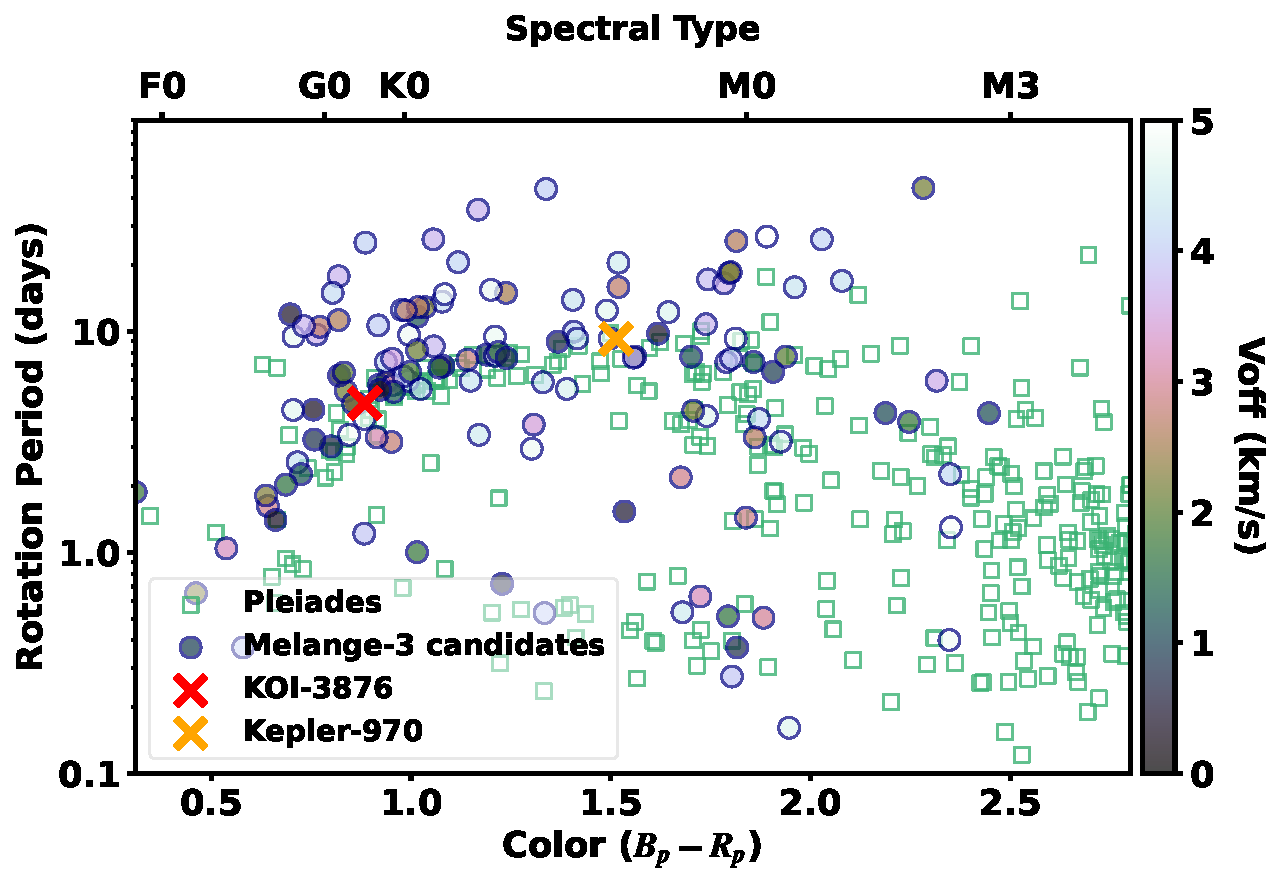
\includegraphics[width=0.47\textwidth, scale = 1.1]{koi3876_cp-seq_final2.pdf}
    \caption{Rotation periods candidate members of \association\ (dark circles). Only literature measurements or stars with Q0 or Q1 rotations are shown. For reference, we show rotation periods from $\simeq$110\, Myr Pleiades (green squares; cite Rebull 2016 Multiperiod Pleiades stars). Stars are color-coded by their tangential velocity difference compared to \starname. Statistically, the stars on the Pleiades gyrochrone are also closer to \starname\ in tangential velocity. Because of the distance to the cluster, we have few rotation periods past M1. 
    \label{fig:rotation}
    }
\end{figure} 





% \subsection{Is this Theia 316??}

% I'm not 100\% sure what needs to go here. We need to either show that this is a part of Theia 316, or that it's not. In some sense it doesn't matter, but we need to address it. 


\section{Parameters of the planet hosts \planetname}\label{sec:stellar_params}

We summarize constraints on the host star in Table~\ref{tab:prop}, the details of which we provide in in this section. 

\subsection{Literature Parameters}
As a reasonably bright ($K_P=12.6$) star hosting a planet candidate from the \kepler\ mission, \starname\ has numerous stellar parameters in the literature. The California \kepler\ Survey estimate \teff=$5720\pm60$\,K, \logg=4.64$\pm$0.1, and \vsini=9.9$\pm$1.0\kms, $R_*0.95^{+0.06}_{-0.04}R_\odot$ and $M_*=1.01\pm0.03M_\odot$ based on comparing their high-resolution spectra and comparison to well-characterized templates \citep{2017AJ....154..107P, 2017ApJ...836...77Y} and stellar isochrones \citep{JohsonCKS2017}. \citet{2018ApJS..237...38B}, using the same spectra, estimate \teff=5642$\pm$27\,K, \logg=$4.46\pm$0.05, $R_*=0.93\pm0.02M_\odot$, $M_*=0.99\pm0.02M_\odot$, and \vsini=10.4$\pm$0.5\kms, as well as detailed abundances that are generally consistent with the Solar value. \citet{2020AJ....160..108B} incorporated \gaia\ DR2 data with MIST stellar isochrones to derive an \teff=$5577\pm85$\,K, \logg$=4.50\pm0.02$, and $R_*=0.908\pm0.017R_\odot$. 

These stellar parameters are generally in agreement with each other. However, those that relied on isochrones \citep{JohsonCKS2017, 2018ApJS..237...38B, 2020AJ....160..108B} assigned $>1$\,Gyr ages, much older than the true $\simeq$80\,Myr age of \starname. Although the assigned errors were large (and hence may be marginally consistent), the derived parameters may still be biased by the lack of an assigned age. Although this will not impact purely spectroscopic parameters like \teff\ and \vsini, the assumption can have a strong impact on the estimated stellar mass. Thus, we revisit these parameters with our own analysis below. 

\subsection{Spectral-Energy Distribution}.

We fit the observed spectral-energy-distribution (SED) following \citet{Mann2016b}. To briefly summarize, we fit the observed photometry with a grid of optical and near-infrared flux-calibrated spectra spanning 0.4--2.3\um. We included BT-SETTL CIFIST atmospheric models \citep{BHAC15} in the fit, both to estimate the \teff\ and fill in gaps in the template spectra (e.g., beyond 2.3\um). We integrated the resulting absolutely-calibrated spectrum to estimate the bolometric flux (\fbol), which we combined with the \gaia\ EDR3 parallax to estimate the stellar luminosity ($L_*$). With \teff\ and $L_*$, we calculated $R_*$ using the Stefan-Boltzmann relation. While reddening in this sight-line is low \citep{2011ApJ...737..103S}, \starname\ is well outside the Local Bubble, so we included extinction as part of the fit. To account for variability in the star, we added (in quadrature) 0.02 mags to the errors of all optical photometry. In total, the fit included six free parameters: the spectral template, $A_V$, three parameters that describe the model ($\log~g$, \teff, and [M/H]), and a scale factor between the model and the photometry. We show an example fit in Figure~\ref{fig:sed}. The resulting fit yielded $A_V=0.16^{+0.10}_{-0.08}$, \teff=$5672\pm65$\,K, \fbol=$(2.55\pm0.10)\times10^{-10}$ (erg\,cm$^{-2}$\,s$^{-1}$), $L_*=0.81\pm0.03L_\odot$, and $R_*=0.94=0.03R_\odot$. 

%AWM: decide later if we actually want this. The scale factor between the atmospheric model and the (de-reddened) photometry is equivalent to $R_*^2/D^2$, and hence provides a separate estimate of the radius when combined with the \gaia\ parallax. This is effectively the infrared-flux method \citep[IRFM, ][]{Blackwell1977}. While not independent of the Stefan-Boltzmann-based radius, it does provide an additional check on our fit. This method yielded a radius of $R_*=0.92=0.02R_\odot$.

Our SED parameters were in good agreement with the literature spectroscopic values. Since the star is Sun-like, we considered the(high-resolution spectroscopic \teff\ to be more reliable than the SED-based value, but the SED-based luminosity (and radius) more reliable than one derived from the spectroscopic \logg\ or isochrone. We combined the two, which yielded a final radius of $0.92\pm0.02R_\odot$.

\subsection{Isochronal parameters}\label{sec:isochrone}
To determine $M_*$ and verify our other stellar parameters, we compared the observed photometry to Solar-metallicity magnetic DSEP evolution models and PARSEC models. We used \texttt{emcee} to simultaneously fit for age, $A_V$, $M_*$, and an additional parameter to capture underestimated uncertainties in the data or models ($f$, in magnitudes) within an MCMC framework. We used a hybrid interpolation method, first identifying the nearest age in then model grid and then performing a linear interpolation in mass to obtain stellar parameters and model photometry. Since this method could not interpolate between ages, we re-sampled the input grid using the \texttt{isochrones} package \citep{2015ascl.soft03010M} to be more dense (0.1\,Myr and 0.01$M_\odot$) than expected errors. To redden the model photometry, we used \texttt{synphot} \citep{pey_lian_lim_2020_3971036} and the extinction law from \citet{1989ApJ...345..245C}. We placed a Gaussian prior on age of 110$\pm$11\,Myr, while other parameters evolved under uniform priors. The resulting fit from each model grid was very precise, but differences between the two grids suggest larger systematic errors. Considering these, the resulting parameters were generally in agreement with our spectroscopic constraints ($R_*=0.968\pm0.07$, $A_V=0.27\pm0.10$, \teff=$5710\pm60$) and provided a stellar mass estimate of $M_*=1.04\pm0.03M_\odot$. We combined this with our earlier radius estimate to get an estimate of the stellar density ($\rho_*=1.30\pm0.10\rho_odot$).

\begin{deluxetable}{lccc}
\centering
\tabletypesize{\scriptsize}
\tablewidth{0pt}
\tablecaption{Properties of the host star \starname. \label{tab:prop}}
\tablehead{\colhead{Parameter} & \colhead{Value} & \colhead{Source} }
\startdata
\multicolumn{3}{c}{Astrometry}\\
\hline
% check parameters on gaia
 $\alpha$  &  290.440629 &  \emph{Gaia} EDR3\\ %updated
 $\delta$. & 38.523572  & \emph{Gaia} EDR3 \\ %updated
 $\mu_\alpha$ (mas\,yr$^{-1}$)& -4.154$\pm$0.010 & \emph{Gaia} EDR3\\ %updated
 $\mu_\delta$  (mas\,yr$^{-1}$) & 2.269$\pm$0.011 & \emph{Gaia} EDR3\\ %updated
 $\pi$ (mas) & 3.0565$\pm$0.0093 & \emph{Gaia} EDR3\\ %updated
\hline
\multicolumn{3}{c}{Photometry}\\
\hline
$G_{Gaia}$ (mag) & 12.6054$\pm0.0028$ & \emph{Gaia} EDR3\\ %updated
$BP_{Gaia}$ (mag) & 12.9642$\pm0.0033$ & \emph{Gaia} EDR3\\ %updated
$RP_{Gaia}$ (mag) & 12.0798$\pm0.0041$ & \emph{Gaia} EDR3\\ %updated
$B$ (mag) & $13.375 \pm 0.094$ & APASS \\ %updated
$V$ (mag) & $12.655 \pm 0.122$ & APASS \\ %updated
$g$' (mag) & $13.038 \pm 0.033$ & APASS \\ %updated
$r$' (mag) & $12.456 \pm 0.092$ & APASS \\ %updated
$i$' (mag) & $12.323 \pm 0.062$ & APASS \\ 
$J$ (mag) & $11.456 \pm 0.02$ &  2MASS\\ %updated
$H$ (mag) & $11.152 \pm 0.016$  & 2MASS\\	 %updated
$K_S$ (mag) & $11.107\pm 0.019$ & 2MASS\\ %updated
$W1$ (mag) & $11.06 \pm 0.023$ & ALLWISE\\%updated
$W2$ (mag)& $11.09 \pm 0.020 $ & ALLWISE\\%updated
$W3$ (mag)& $10.91 \pm 0.094$ & ALLWISE\\ %updated
\hline
\multicolumn{3}{c}{Kinematics \& Position}\\
\hline
RV$_{\rm{Bary}}$ (km\, s$^{-1}$) & -26.79$\pm$0.01 & \citet{2020AJ....160..120J}\\ %updated
%U (km\, s$^{-1}$) & 13.66$\pm$0.09 & This work\\
%V (km\, s$^{-1}$) & 2.42$\pm$0.02 & This work\\
%W (km\, s$^{-1}$) & -7.75$\pm$0.04 & This work\\
%X (pc) & -19.89$\pm$0.02 & This work\\
%Y (pc) & -4.697$\pm$0.005 & This work\\
%Z (pc) & 9.164$\pm$0.091 & This work\\
\hline
\multicolumn{3}{c}{Physical Properties}\\
\hline
$P_{\rm{rot}}$ (days) &  $4.69\pm0.04$ & \citep{2014ApJS..211...24M}\\
%$\log R'_{\rm{HK}}$ & $-4.39\pm0.05$ & This work\\
\vsini (km\, s$^{-1}$) & $ 10.4\pm0.5 $ & \citet{2018ApJS..237...38B}\\ %updated
$i_*$ ($^\circ$) & $ >80$ & This work\\
\fbol\,(erg\,cm$^{-2}$\,s$^{-1}$)& $(2.55\pm0.10)\times10^{-10}$ & This work\\  %updated
\teff\ (K) & $5720 \pm 60$ & This work, CKS\\ %updated
%\logg\ (dex) & $4.45\pm0.10$ & This work\\
\textup{[Fe/H]} & $0.12\pm0.02$ & \citet{2018ApJS..237...38B}\\ %updated
M$_\star$ (M$_\odot$) & $ 1.01\pm0.03 $ & This work \\ %updated
R$_\star$ (R$_\odot$) &  $ 0.92\pm0.02 $ & This work \\ %updated
L$_\star$ (L$_\odot$) & $ 0.81\pm0.03 $ & This work \\ %updated
$\rho_\star$ ($\rho_\odot$) & $1.30\pm0.10$ & This work \\ %updated
Age (Myr) & $110\pm11$  & This work %updated
\enddata
\end{deluxetable}



\begin{figure}[tb]
    \centering
    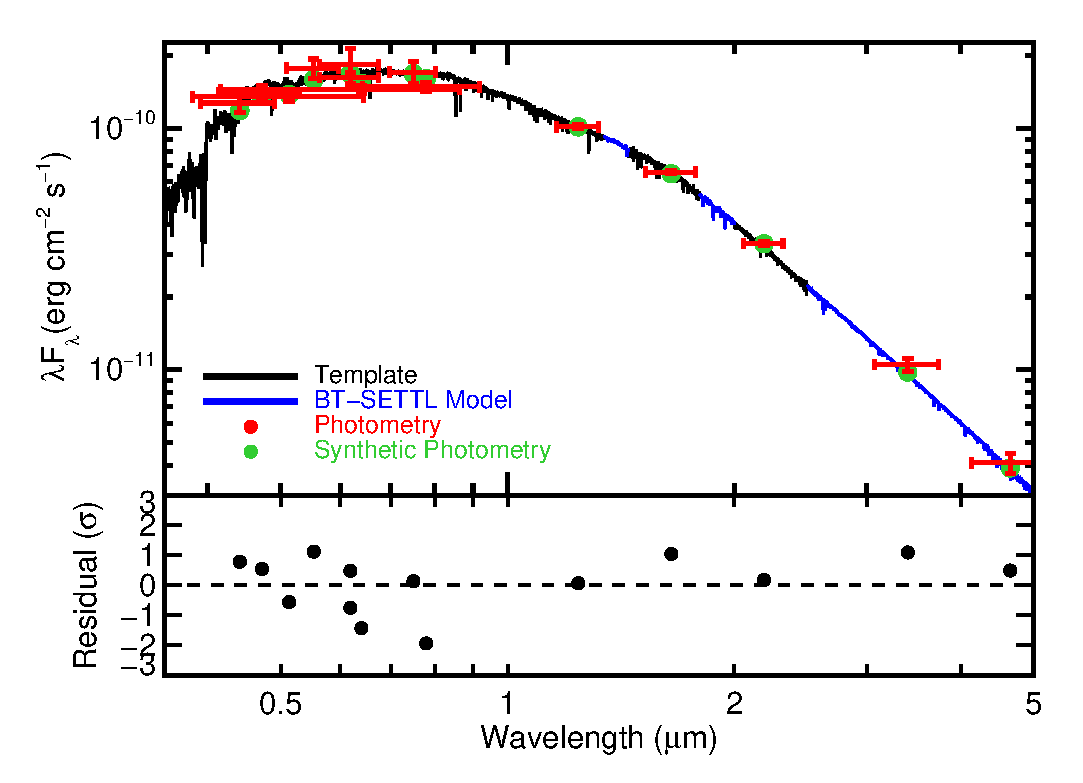
\includegraphics[width=0.49\textwidth]{KOI3876_SED.eps}
    \caption{Best-fit template spectrum (G1V; black) and synthetic photometry (green) compared to the observed photometry of \starname\ (red). Errors on observed photometry are shown as vertical error bars, while horizontal error bars indicate the approximate width of the filter. BT-SETTL models (blue) were used to fill in regions of high telluric absorption or beyond the template range. The bottom panel shows the photometric residual in units of standard deviations. }
    \label{fig:sed}
\end{figure} 


\subsection{Stellar inclination}\label{sec:inc}

To test whether the stellar spin and planetary orbit are consistent with alignment, we computed the stellar inclination ($i_*$) from the \vsini, $P_{\rm{rot}}$, and $R_*$ values estimated above. In is simplest form, this calculation is $V=2\pi R_*/P_{\rm{rot}}$, but requires additional statistical corrections \citep[see ][]{MortonWinn2014, 2020AJ....159...81M}. Here we followed the methodology described in \citet{2020AJ....159...81M}. The resulting stellar inclination was $i_*>71^\circ$ at 95\% confidence and $i_*>80^\circ$ at 68\% confidence. This is consistent with alignment with \planetname's orbital inclination. 

\section{Parameters of \planetname}\label{sec:transit}

We fit the \kepler\ photometry using the \texttt{misttborn} (MCMC Interface for Synthesis of Transits, Tomography, Binaries, and Others of a Relevant Nature) fitting code\footnote{\url{https://github.com/captain-exoplanet/misttborn}} first described in \citet{Mann2016a} and expanded upon in \citet{MISTTBORN}. \texttt{misttborn} uses \texttt{BATMAN} \citep{Kreidberg2015} to generate model light curves and \texttt{emcee} \citep{Foreman-Mackey2013} to explore the transit parameter space. 

The standard implementation of \texttt{misttborn} fits for six parameters for each transiting planet: time of periastron ($T_0$), orbital period of the planet ($P$), planet-to-star radius ratio ($R_p/R_\star$), impact parameter ($b$), and stellar density ($\rho_\star$). For each wavelength observed, we fit two linear and quadratic limb-darkening coefficients ($q_1$, $q_2$) following the triangular sampling prescription of \citet{Kipping2013}. To cover all four bands (\textit{TESS} and SDSS $griz$) required ten limb-darkening parameters in total. Gas drag and gravitational interactions are expected to dampen out eccentricities and inclinations of extremely young planets like \planetname\ \citep{2004ApJ...602..388T}, so we locked the eccentricity at zero.

We ran two versions of the fit. In the first, the MCMC chain restricted $e$ to 0 and allowed $\rho_\star$ to vary within a uniform distribution, and the second allowed $e$ to vary with a Gaussian prior on $\rho_\star$ from our spectroscopic and SED analysis (Section~\ref{sec:stellar_params}). For both fits, applied Gaussian priors on the limb-darkening coefficients based on the values derived using our stellar parameters from Section~\ref{sec:stellar_params} and the \texttt{LDTK} toolkit \citet{2015MNRAS.453.3821P}, with errors accounting for the difference between models (0.42$\pm$0.08 and 0.13$\pm$0.04 for linear and quadratic terms, respectively). All other parameters were sampled uniformly with physically motivated boundaries; e.g., $T_0$ was restricted to the time period sampled by the data and $|b|<1+R_P/R_*$.

To model stellar variations, \texttt{misttborn} includes a Gaussian Process (GP) regression module, utilizing the \texttt{celerite} code \citep{celerite}. We used a mixture of two stochastically driven damped simple harmonic oscillators (SHOs) at periods $P_{GP}$ (primary) and $0.5P_{GP}$ (secondary). In total, there were five GP parameters: the log of the dominant period ($\ln(P_{GP})$), the log of the GP amplitude ($\ln{\rm{Amp}}$), a decay timescale for the variability (quality factor, $\ln{Q0}$), the difference between the primary and secondary quality factors ($\ln{\Delta Q}$), and a mix parameter that describes how the primary and secondary signals are combined (Mix). All GP parameters evolved under uniform priors. 

We ran the MCMC using 50 walkers for 250000 steps including a burn-in of 20000 steps. The total run was more than 50 times the autocorrelation time (for both fits), indicating that the total run was sufficient for convergence.

As we show in Figures~\ref{fig:quarter2GP}, the SHOs GP did an excellent job describing the overall variability, even in the presence of complex changes in the light curve morphology during the 4.5 years it was observed by \kepler. We also show the phase folded light curve in Figure \ref{fig:ecctransit} for the fit where $e$ was allowed to vary. The best-fit parameters with uncertainties for both fits can be found in Table \ref{tab:bestfitParams}, and the corner plot for the major transit-fit parameters for the eccentric fit is in Figure \ref{fig:ecccorner}. 

The first fit ($e=0$) yields a $\rho_{\star}$ value much larger than the spectroscopic/isochronal value determined in Section~\ref{sec:stellar_params} (15.5$\rho_\odot$ vs 1.3$\rho_\odot$). Although the error on the transit-fit density is large (5.9$\rho_\odot$), so the two values are consistent at $\simeq2.5\sigma$. But this suggests the planet is likely to be eccentric. Indeed, in the fit where $e$ is allowed to float, the preferred $e$ is 0.2--0.4. For this reason, we adopt the second fit, where $e$ is allowed to float, as the preferred fit.  

\begin{figure*}[tb]
    \centering
    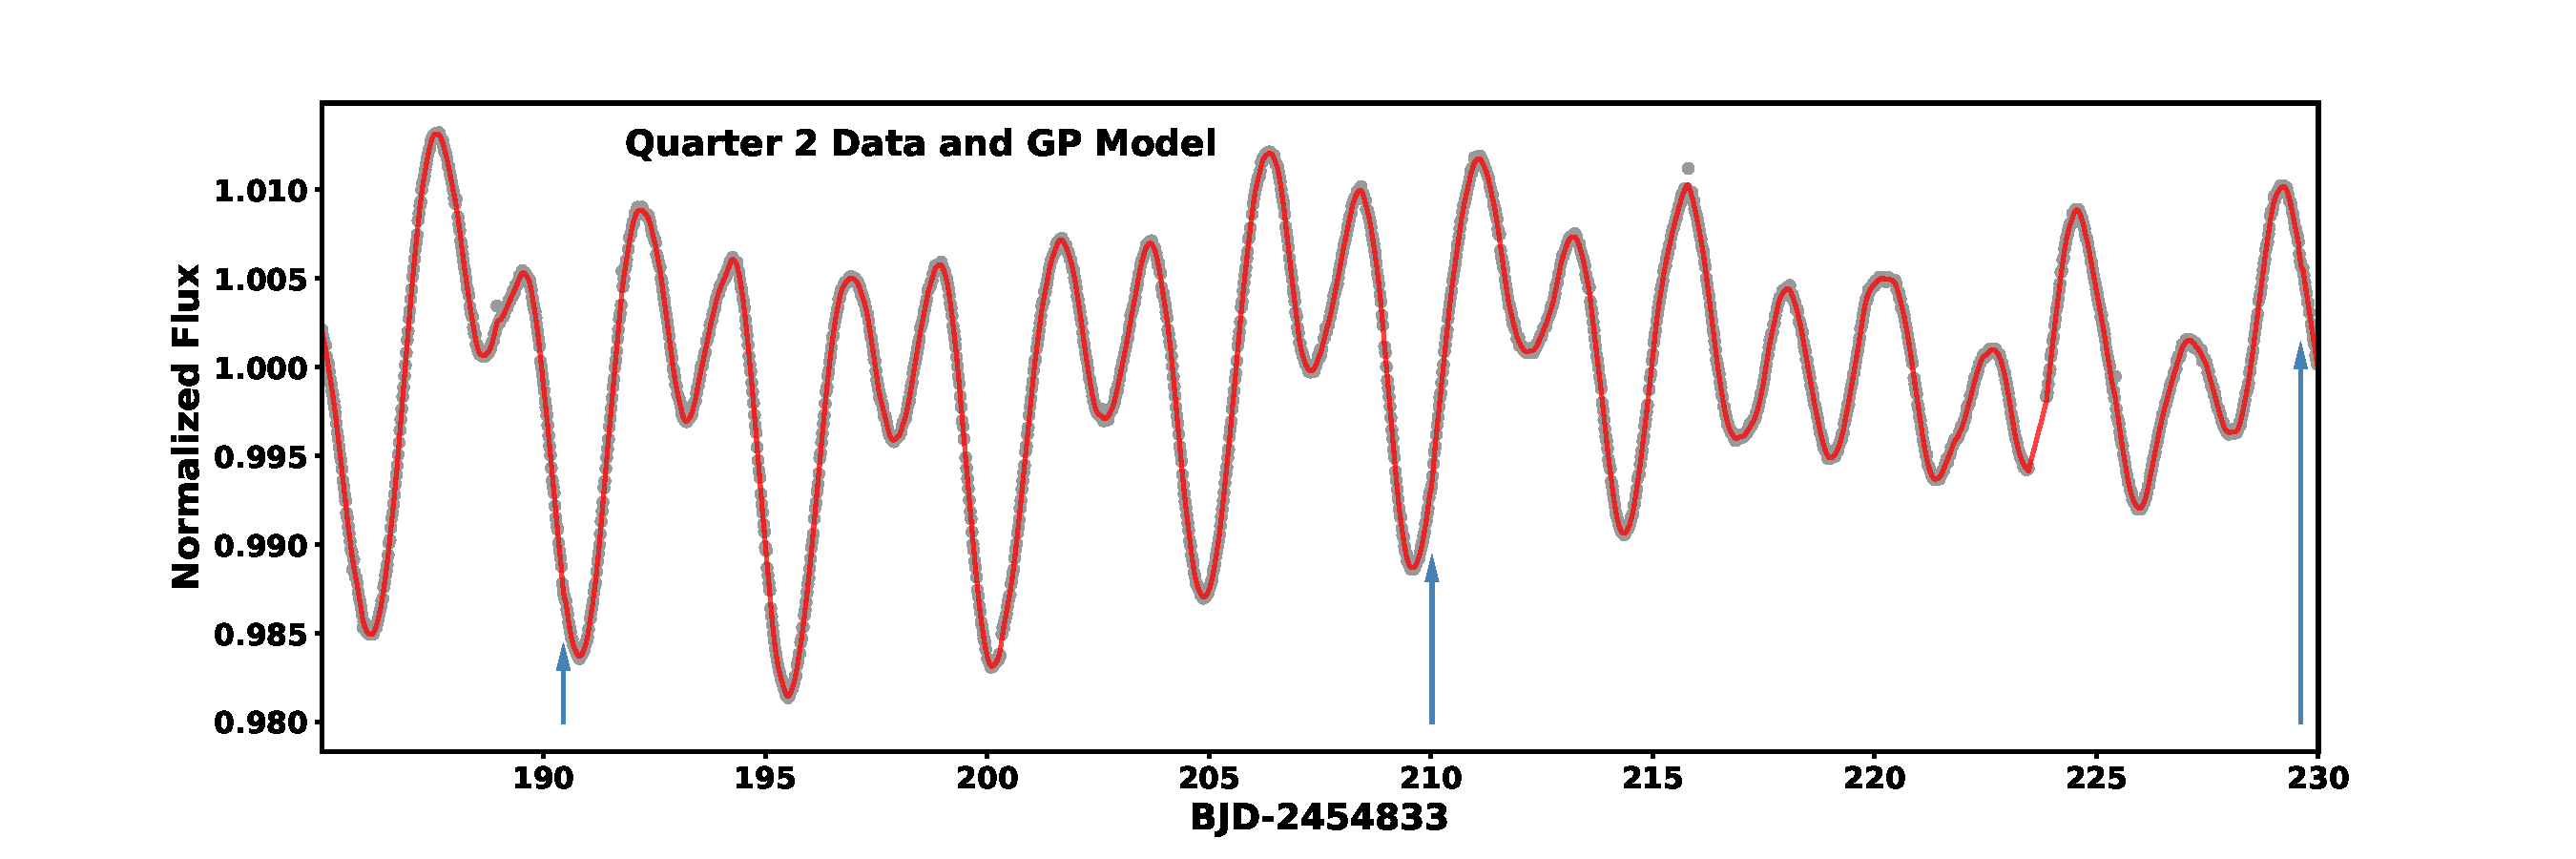
\includegraphics[trim=50 0 50 0,clip=True,width=\textwidth]{q2GP.pdf}
    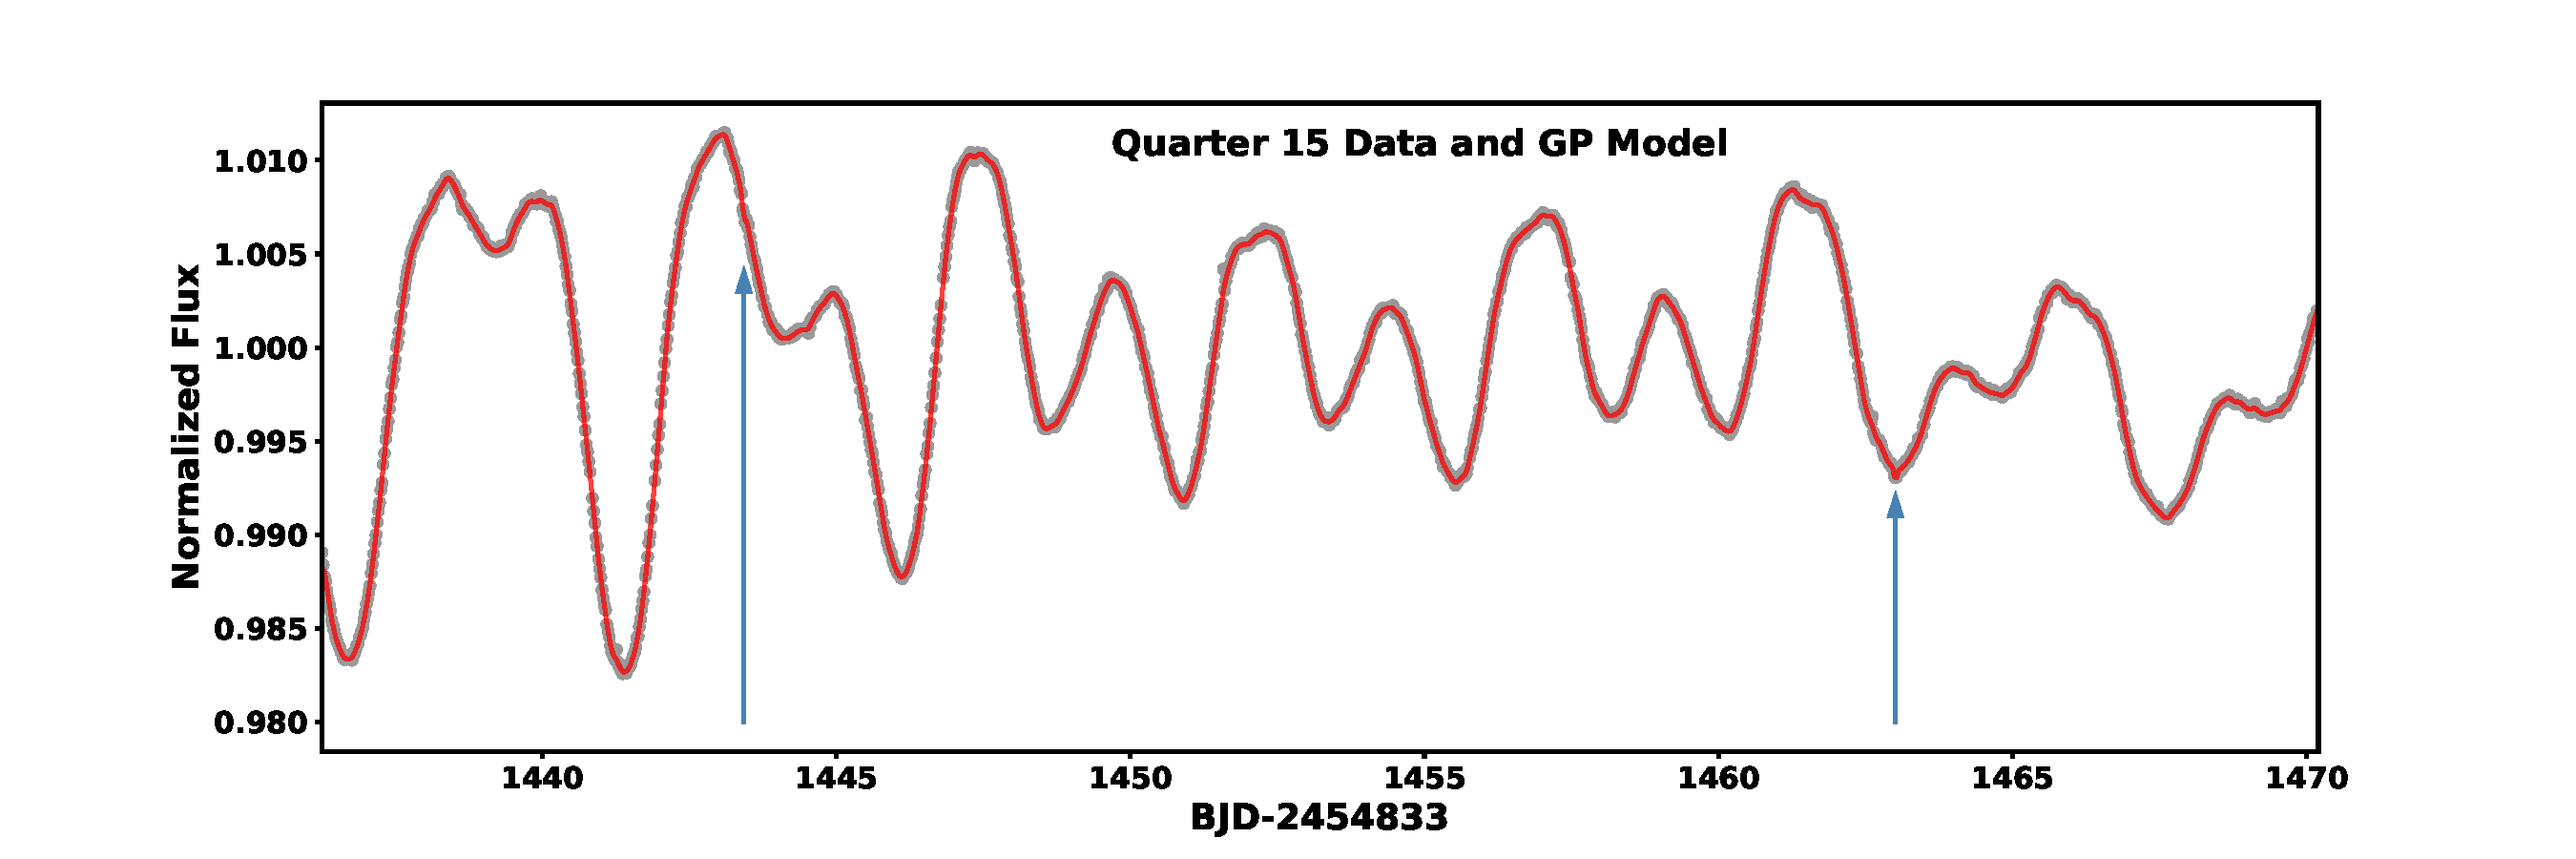
\includegraphics[trim=50 0 50 0,clip=True, width=\textwidth]{q15GP.pdf}
    \caption{Approximately 40-day windows from \kepler\ Quarter 2 (top) and \kepler\ Quarter 15 (bottom) light curve of \starname. The normalized flux (grey) is shown with our best-fit GP model (red). The locations of transits are shown with the blue arrows.}
    \label{fig:quarter2GP}
\end{figure*} 

% limb darkening from ldtk:
% g1 = 0.4247
% g2 = 0.1271
% g1err = 0.08
% g2err = 0.04


% to be updated soon
\begin{figure}[tb]
    \centering
    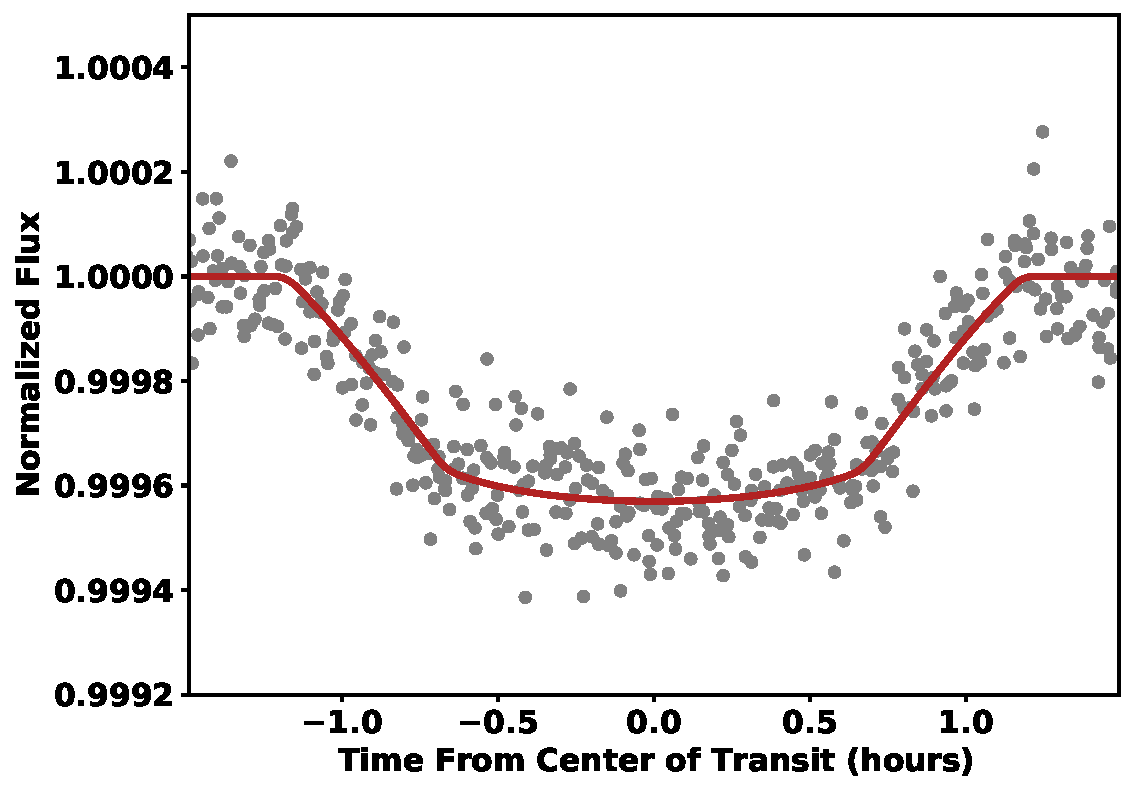
\includegraphics[width=0.49\textwidth]{eccTransit.pdf}
    \caption{Phase-folded light curve of \starname\ from \kepler\ (grey points) with the best-fit transit model (red). The best-fit GP model to the stellar variability has been removed from both the data and the model for clarity. P}
    \label{fig:ecctransit}
\end{figure} 

% ecc corner
\begin{figure}[tb]
    \centering
    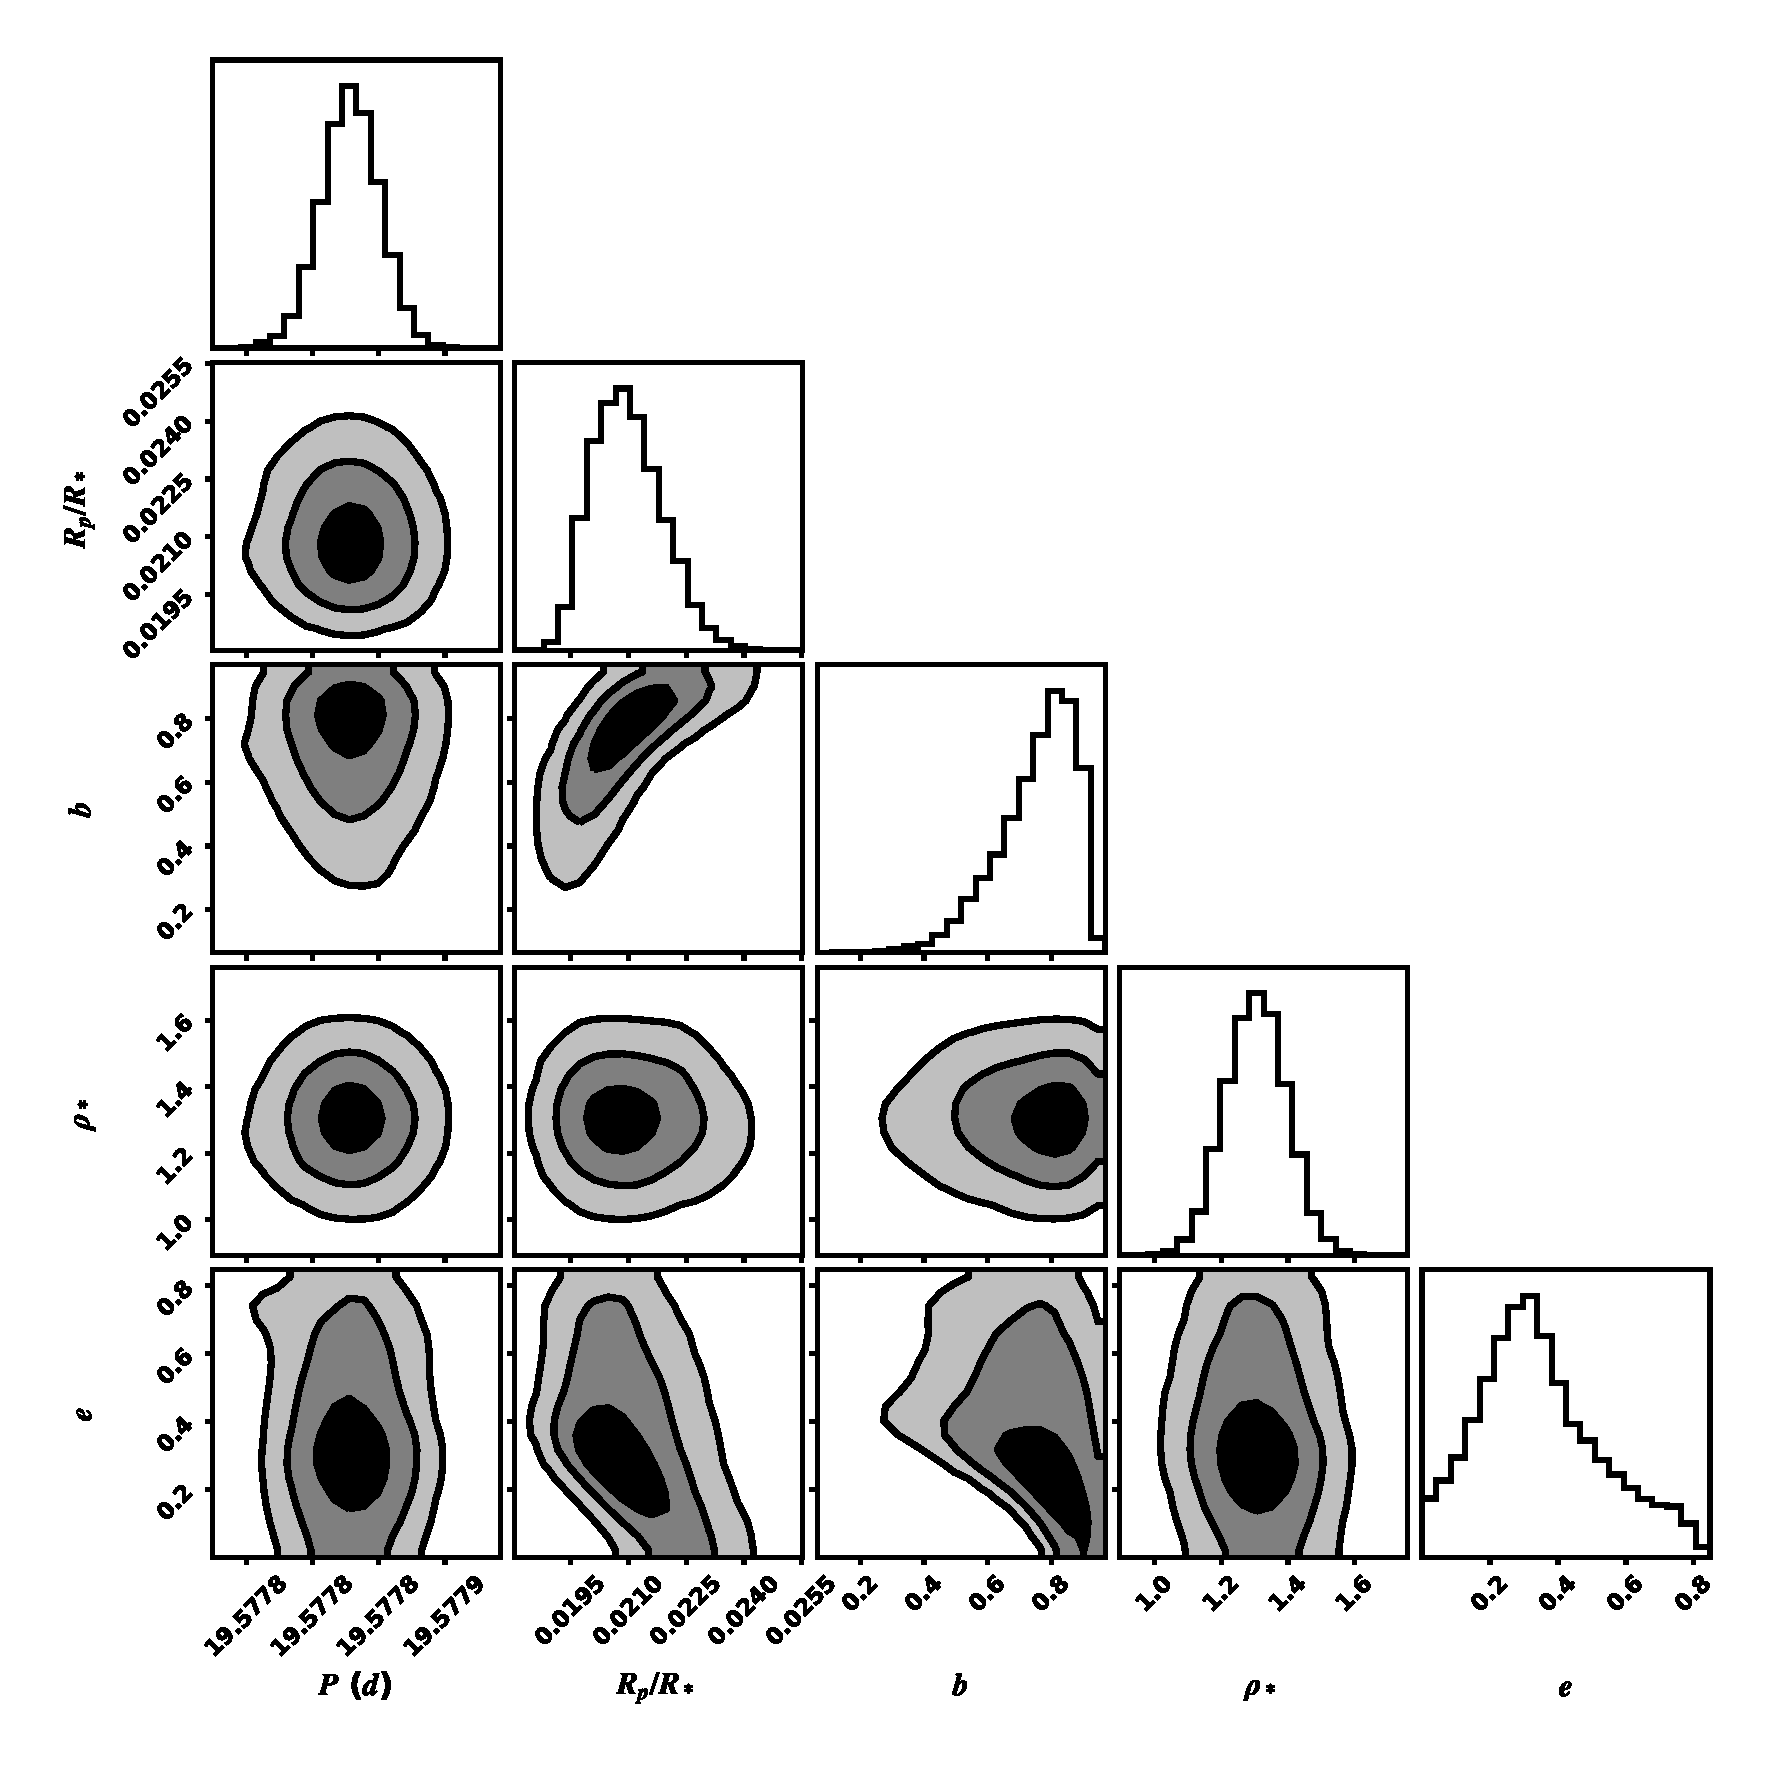
\includegraphics[width=0.49\textwidth]{KOI3876_corner1_3sig.pdf}
    \caption{Corner plot of the major transit parameters ($P$, $R_P/R_*$, $b$, $\rho_*$, and $e$) from our \texttt{MISTTBORN} fit. The contour levels correspond to 1$\sigma$, 2$\sigma$, and 3$\sigma$ of the points (from darkest to lightest). The planet-to-star radius ratio and eccentricity are strongly covariant with impact parameter, as a higher impact parameter requires a deeper transit (and lower eccentricity) to reproduce the observed transit depth (and duration). Plot made using {\texttt corner.py} \citep{foreman2016corner}.}
    \label{fig:ecccorner}
\end{figure} 



\begin{deluxetable*}{lccc}
\centering
\tabletypesize{\scriptsize}
\tablewidth{0pt}
\tablecaption{Parameters of \starname \label{tab:bestfitParams}
}
\tablehead{
\colhead{Parameter} & \multicolumn{2}{c}{Values}\\%\colhead{Values} & \colhead{Value}\\ 
\colhead{} & \colhead{e=0} & \colhead{e float (preferred)}
}
\startdata
\multicolumn{3}{c}{Measured Parameters }\\
\hline
$T_0$ (BJD-2454833) & $131.71494 \pm 0.00087$ & $131.71488^{+0.00089}_{-0.0009}$\\ 
$P$ (days) & $19.577829 \pm 2.1\times10^{-5}$ & $19.57783^{+2.2\times10^{-5}}_{-2.3\times10^{-5}}$\\ 
$R_P/R_{\star}$ & $0.01946^{+0.00061}_{-0.00043}$ & $0.02112^{+0.00092}_{-0.00079}$\\ 
$b$ & $0.31^{+0.28}_{-0.22}$ & $0.803^{+0.081}_{-0.1}$\\ 
$\rho_{\star}$ ($\rho_{\odot}$) & $15.5^{+2.5}_{-5.9}$ & $1.308^{+0.09}_{-0.089}$\\ 
$q_{1,1}$ & $0.291^{+0.107}_{-0.099}$ & $0.305^{+0.101}_{-0.096}$\\ 
$q_{2,1}$ & $0.371^{+0.075}_{-0.086}$ & $0.373^{+0.077}_{-0.09}$\\
$\sqrt{e}\sin\omega$ & -- & $0.29^{+0.16}_{-0.22}$ \\ 
$\sqrt{e}\cos\omega$ & -- & $-0.07 \pm 0.48$ \\ 
$\log(P_{GP})$ & $1.5658 \pm 0.0036$ & $2.09^{+0.012}_{-0.5}$\\ 
$\log(Amp)$ & $-9.48^{+0.13}_{-0.12}$ & $-9.348^{+0.095}_{-0.2}$\\ 
$\log(\Delta Q)$ & $2.41 \pm 0.22$ & $108.7^{+170.0}_{-110.0}$ \\ 
$\log(Q0)$ & $1.36^{+0.059}_{-0.056}$ & $1.195^{+0.162}_{-0.08}$\\ 
$\log(Mix)$ & $-1.56^{+0.16}_{-0.17}$ & $3.6^{+4.2}_{-5.1}$\\ 
\hline 
\multicolumn{3}{c}{Derived Parameters }\\
\hline
$a/R_{\star}$ & $76.2^{+3.9}_{-10.0}$ & $40.2^{+4.1}_{-4.4}$\\ 
$i$ ($^{\circ}$) & $89.76^{+0.17}_{-0.29}$ & $88.56^{+0.19}_{-0.13}$\\ 
% $\delta$ (\%) & $0.0379^{+0.0024}_{-0.0017}$ & $0.0446^{+0.0039}_{-0.0033}$\\ 
$T_{14}$ (days) & $0.0794^{+0.0016}_{-0.0015}$ & $0.097^{+0.044}_{-0.019}$\\ 
$T_{23}$ (days) & $0.0756^{+0.0015}_{-0.0016}$ & $0.085^{+0.042}_{-0.02}$\\ 
% FPP parameter & $0.22^{+0.72}_{-0.2}$ & $2.26^{+1.07}_{-0.88}$\\ 
% $T_{\mathrm{peri}}$ (BJD) & $131.71494 \pm 0.00087$ & $132.1^{+1.5}_{-2.2}$\\ 
% $g_{1,1}$ & $0.39^{+0.11}_{-0.1}$ & $0.4^{+0.11}_{-0.12}$\\ 
% $g_{2,1}$ & $0.133^{+0.104}_{-0.08}$ & $0.136^{+0.107}_{-0.085}$\\ 
% $R_P$ ($R_J$) & $0.1741^{+0.0066}_{-0.0054}$ & $0.182 \pm 0.026$\\ 
$a$ (AU) & $0.326^{+0.018}_{-0.049}$ & $0.165 \pm 0.029$\\ 
% $T_{\mathrm{eq}}$ (K) & $463.0^{+35.0}_{-13.0}$ & $627.0^{+36.0}_{-34.0}$\\ 
% $S$ ($S_{\oplus})$ & $7.69^{+2.32}_{-0.84}$ & $25.8^{+6.0}_{-5.6}$\\
$e$ & \ldots & $0.27^{+0.16}_{-0.14}$ \\ 
$\omega$ ($^{\circ}$) & \ldots & $114.0^{+55.0}_{-73.0}$ \\
\hline 
\enddata
\end{deluxetable*}




\subsection{False Positive Analysis}\label{sec:fpp}
In \citet{2016ApJ...822...86M}, the authors run the false-positive probability calculator \texttt{VESPA} \citet{2015ascl.soft03011M} on all \kepler\ objects of interest available at the time, which included \planetname. They assigned a high probability that \planetname\ (90\%) that \planetname\ is an eclipsing binary, and $<1\%$ that the signal is due to a planet overall. This conclusion was based primarily on the light curve morphology and available stellar parameters.

\begin{figure*}[tb]
    \centering
    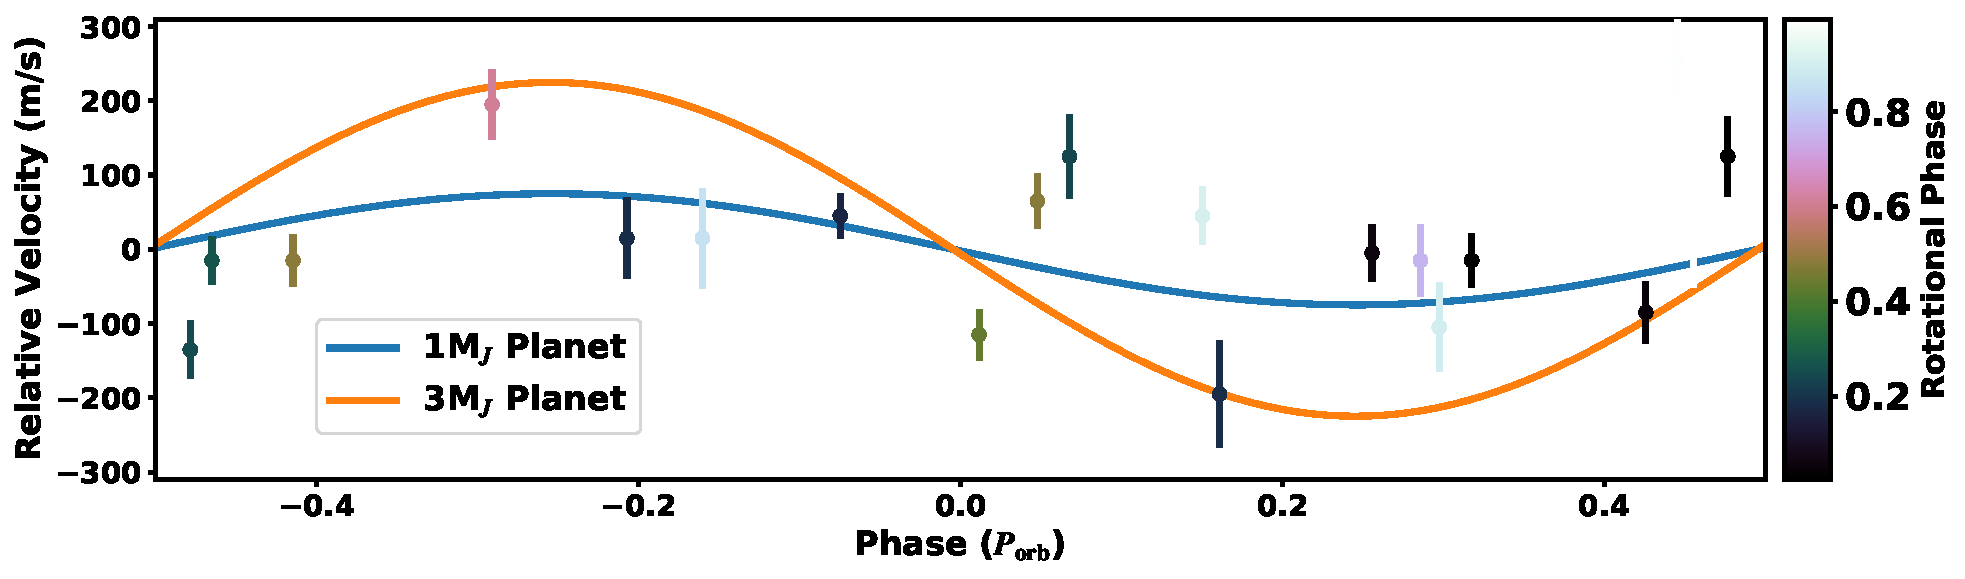
\includegraphics[width=0.99\textwidth]{APOGEE_RVs.pdf}
    \caption{Radial velocities from APOGEE \citep{2020AJ....160..120J} for \starname\ as a function of the planet's orbital phase and colored by the rotational phase. The velocities rule out any companion more massive than $\simeq2M_J$, ruling out any possibility of an eclipsing binary at the transit period. The scatter is larger than expected for the uncertainties by $\simeq$100\mps, but this is most likely due to stellar jitter common in young stars \citep{2019A&A...632A..37B, 2021AJ....161..173T}, and this is still far below the expected variation for a tight eclipsing binary. }
    \label{fig:RVs}
\end{figure*} 


 As we show in Figure~\ref{fig:RVs}, radial velocities from the Apache Point Observatory Galactic Evolution Experiment 16th data release \citep[APOGEE DR16;][]{2020AJ....160..120J} rule out any stellar companion at the period of the planet. Further, our light curve analysis shows the expected U-shape transit for a planet, and there is no sign of a companion in the extant spectroscopy or adaptive optics imaging and non-redunant aperture masking from \citet{Kraus2016a}. \gaia\ EDR3 astrometry and imaging similarly shows no sign of a companion. There is only one star detected with the \kepler\ PSF, which is too faint to reproduce the transit. 
 
 \starname\ also has a low Renormalised Unit Weight Error (RUWE) in EDR3 (0.94)
 
 RUWE value is effectively an astrometric reduced $\chi^2$ value, normalized to correct for color and brightness dependent effects\footnote{\url{https://gea.esac.esa.int/archive/documentation/GDR2/Gaia_archive/chap_datamodel/sec_dm_main_tables/ssec_dm_ruwe.html}}. RUWE should be around 1 for well-behaved sources, and higher values (RUWE$\gtrsim$1.3) suggests with the presence of a stellar companion \citep{Ziegler2020, 2021arXiv210609040W}. 
 
 It is possible the high \citet{2016ApJ...822...86M} was an artifact of poor detrending of the high stellar variability in \starname\ and/or the mismatch between the transit duration and that expected for a circular orbit (see Section~\ref{sec:transit}). This motivated a 

Rerunning the \texttt{VESPA} analysis, we find a 97\% probability \planetname\ is a planet and a 3\% probability \planetname\ is an eclipsing binary. As previously stated, shown in Figure \ref{fig:RVs}, a stellar companion to \starname\ is ruled out at the period of the planet. Therefore, we conclude \planetname\ is a planet.

\textcolor{red}{AWM: do we want to say something about the AO imaging somewhere}. 

% run Tri on 3876

\section{Summary and Conclusions}\label{sec:summary}
\planetname\ is a $\simeq$ 110 Myr planet in the newly identified \association\ association. \planetname\ is about twice the size of the earth, orbiting a star that is a young analog to the Sun, having a similar radius and mass. Originally flagged as a false positive by //false positive work//, we rule out this disposition based on APOGEE radial velocities and our own light curve analysis. We see that the radial velocity dispersion of the system is not well-modeled by a stellar-mass body, ruling out the possibility of an eclipsing binary. The scatter in radial velocity is likely due to the stellar jitter that is common in young stars since the variation is still below expected for even a tight eclipsing binary.

We used rotation periods, lithium, and isochronal evolution models in order to age \association\, and thus \planetname\, to $110\pm10$ Myr. Based on //theia work//, we conclude that \association may(not) be a subgroup of the larger Theia 316 association. //Theia 316 conclusion// Due to the high number of stars too faint for radial velocity and Lithium follow-up, it is uncertain whether or not these groups overlap.

Using misttborn, we find that \planetname\ likely has an eccentric orbit. We find that we can only match the fitted stellar density and the estimated isochronal density by allowing the eccentricity to vary in the fit rather than fixing it to 0. Because of this, we prefer the eccentric fit parameters over the fixed eccentricity fit. 

Further, we identified additional candidates in the association for future follow-up that have potential of being planetary candidates. Due to the low SNR of the targets, we simply call these candidates in need of follow up. 

\begin{acknowledgements}
The THYME collaboration would like to acknowledge Halee, who kept Madyson sane during lockdown.

MGB was supported by the NC Space Grant Undergraduate Research program and by funding from the Chancellor's Science Scholars Program at the University of North Carolina at Chapel Hill.
%% thank the CSS and NC Space grant
%% Thank whatever paid Andrew over the Summer

%AWM was supported through NASA’s Astrophysics Data Analysis Program (80NSSC19K0583). MLW was supported by a grant through NASA's \ktwo\ GO program (80NSSC19K0097). This material is based upon work supported by the National Science Foundation Graduate Research Fellowship Program under Grant No. DGE-1650116 to PCT. AV's work was performed under contract with the California Institute of Technology/Jet Propulsion Laboratory funded by NASA through the Sagan Fellowship Program executed by the NASA Exoplanet Science Institute. D. D. acknowledges support from NASA through Caltech/JPL grant RSA-1006130 and through the TESS Guest Investigator Program Grant 80NSSC19K1727.

%This paper includes data collected by the TESS mission, which are publicly available from the Mikulski Archive for Space Telescopes (MAST). Funding for the TESS mission is provided by NASA’s Science Mission directorate. This research has made use of the Exoplanet Follow-up Observation Program website, which is operated by the California Institute of Technology, under contract with the National Aeronautics and Space Administration under the Exoplanet Exploration Program. This work has made use of data from the European Space Agency (ESA) mission \emph{Gaia} \footnote{\url{https://www.cosmos.esa.int/gaia}}, processed by the \emph{Gaia} Data Processing and Analysis Consortium (DPAC)\footnote{\url{https://www.cosmos.esa.int/web/gaia/dpac/consortium}}. Funding for the DPAC has been provided by national institutions, in particular the institutions participating in the \emph{Gaia} Multilateral Agreement.  This research has made use of the VizieR catalogue access tool, CDS, Strasbourg, France. The original description of the VizieR service was published in A\&AS 143, 23. Resources supporting this work were provided by the NASA High-End Computing (HEC) Program through the NASA Advanced Supercomputing (NAS) Division at Ames Research Center for the production of the SPOC data products. We acknowledge the use of public TOI Release data from pipelines at the TESS Science Office and at the TESS Science Processing Operations Center. Based on data retrieved from the SOPHIE archive at Observatoire de Haute-Provence (OHP), available at atlas.obs-hp.fr/sophie. This work makes use of observations from the LCOGT network. Based on observations made with the Italian {\it Telescopio Nazionale Galileo} (TNG) operated by the {\it Fundaci\'on Galileo Galilei} (FGG) of the {\it Istituto Nazionale di Astrofisica} (INAF) at the {\it Observatorio del Roque de los Muchachos} (La Palma, Canary Islands, Spain). Part of this research was carried out at the Jet Propulsion Laboratory, California Institute of Technology, under a contract with the National Aeronautics and Space Administration (NASA). The HARPS-N project has been funded by the Prodex Program of the Swiss Space Office (SSO), the Harvard University Origins of Life Initiative (HUOLI), the Scottish Universities Physics Alliance (SUPA), the University of Geneva, the Smithsonian Astrophysical Observatory (SAO), and the Italian National Astrophysical Institute (INAF), the University of St Andrews, Queens University Belfast, and the University of Edinburgh.
\end{acknowledgements}

%\vspace{5mm}
%\facilities{TESS, LCOGT 1m (Sinistro), LCOGT 1m (NRES), SMARTS 1.5m (CHIRON), Tillinghast 1.5m (TRES), SOAR (Goodman), TNG (HARPS-N), OHP 1.93m (ELODIE), OHP 1.93m (SOPHIE), Shane 3m (Hamilton), \ldots}


%\software{\texttt{LcTools}, \texttt{misttborn.py}, \textit{emcee} \citep{Foreman-Mackey2013}, \textit{batman} \citep{Kreidberg2015}, matplotlib \citep{hunter2007matplotlib}, \texttt{corner.py} \citep{foreman2016corner}, \texttt{AstroImageJ} \citep{Collins17}, BANZAI \citep{McCully18}
%          }

\bibliography{fullbiblio}{}
\bibliographystyle{aasjournal}

\clearpage

%% what goes in this table?
%% Name, EDR3 ID, RA, Dec, SpT(phot), Lithium, Friend?, Banyan prob
%% do we want to denote the ones from:
%--https://ui.adsabs.harvard.edu/abs/2008hsf2.book..757T/abstract
%--https://ui.adsabs.harvard.edu/abs/2013MNRAS.435.1325M/abstract
%--https://arxiv.org/abs/2011.06621
%--https://ui.adsabs.harvard.edu/abs/2020AJ....159..166U/abstract
%--https://arxiv.org/abs/2102.05589
%--https://arxiv.org/abs/1807.02076 (this is the Crux one). 


%% Table Notes / Questions
% need to add updated prots
% too many columns...
% cut off sides and end
% Should I cut list based on the old caption (10pc, 1km/s)?
% fix column headings (after final table inserted)
% changing source from name to citation (?)
%\startlongtable
%\begin{rotatetable*}
\begin{longrotatetable}
\begin{deluxetable*}{cccccccccccccccccc}
\tablehead{
\colhead{Gaia EDR3} & \colhead{$\alpha$} & \colhead{$\delta$} & \colhead{Gmag} & \colhead{$V_{\rm{off}}$} & \colhead{Spectral} & \colhead{TESS} & \colhead{Kepler} & \colhead{$\pi$} & \colhead{$\sigma_\pi$} & \colhead{$P_{\rm{rot}}$} & \colhead{$\sigma_{P_{\rm{rot}}}$} & \colhead{$P_{\rm{rot}}$} & \colhead{Li} & \colhead{$\sigma_{\rm{li}}$} & \colhead{RV} & \colhead{$\sigma_{\rm{RV}}$} & \colhead{RV}\\
\colhead{} & \colhead{(J2016)} & \colhead{(J2016)} & \colhead{(mag)} & \colhead{(km/s)} & \colhead{Class} & \colhead{} & \colhead{} & \colhead{(mas)} & \colhead{(mas)} & \colhead{(days)} & \colhead{(days)} & \colhead{ref} & \colhead{($m\AA$)} & \colhead{($m\AA$)} & \colhead{(km/s)} & \colhead{(km/s)} & \colhead{ref}\label{tab:sample}
}
\startdata
2052827207364859264 & 290.44063 & 38.52357 & 12.605 & 0.000 & G7.3 & Y & Y & 3.057 & 0.009 & 4.69 & 0.044 & 2 & 134.0 & 18.0 & -26.088 & 0.026 & 5 \\
2052804323776522624 & 290.46921 & 38.20201 & 18.977 & 3.554 & M3.9 & N & N & 3.036 & 0.172 & $\ldots$ & $\ldots$ & $\ldots$ & $\ldots$ & $\ldots$ & $\ldots$ & $\ldots$ & $\ldots$ \\
2100939194794324608 & 289.80783 & 38.95042 & 10.829 & 0.478 & F4.4 & Y & N & 3.024 & 0.012 & $\ldots$ & $\ldots$ & $\ldots$ & $<$20 & $\ldots$ & -27.027 & 0.184 & 5 \\
2052954995531623040 & 291.28017 & 39.20070 & 14.355 & 4.348 & K4.7 & N & Y & 3.055 & 0.016 & 13.849 & 0.386 & 1, 2, 3 & $\ldots$ & $\ldots$ & $\ldots$ & $\ldots$ & $\ldots$ \\
2100967537279486336 & 290.14895 & 39.26079 & 18.451 & 3.806 & M4.1 & N & N & 3.094 & 0.136 & $\ldots$ & $\ldots$ & $\ldots$ & $\ldots$ & $\ldots$ & $\ldots$ & $\ldots$ & $\ldots$ \\
2051102868195719168 & 290.43983 & 37.73210 & 17.503 & 0.516 & M3.2 & N & N & 3.019 & 0.069 & $\ldots$ & $\ldots$ & $\ldots$ & $\ldots$ & $\ldots$ & $\ldots$ & $\ldots$ & $\ldots$ \\
2053037660761796096 & 290.86832 & 39.65124 & 17.902 & 0.605 & M3.7 & N & N & 3.067 & 0.084 & $\ldots$ & $\ldots$ & $\ldots$ & $\ldots$ & $\ldots$ & $\ldots$ & $\ldots$ & $\ldots$ \\
2052645379929910144 & 290.91118 & 38.33558 & 13.747 & 0.988 & K2.8 & N & Y & 2.996 & 0.033 & 5.264 & $\ldots$ & 4 & $\ldots$ & $\ldots$ & -34.923 & 3.954 & 6 \\
2052559995978462208 & 291.61221 & 37.79730 & 11.75 & 3.744 & F9.3 & Y & Y & 3.082 & 0.01 & 10.94 & 0.151 & 1 & $\ldots$ & $\ldots$ & -16.07 & 0.95 & 7 \\
2100996639982248320 & 289.86923 & 39.64549 & 19.678 & 2.692 & M3.7 & N & N & 3.083 & 0.322 & $\ldots$ & $\ldots$ & $\ldots$ & $\ldots$ & $\ldots$ & $\ldots$ & $\ldots$ & $\ldots$ \\
2099426507311747200 & 289.44803 & 38.58778 & 17.385 & 0.897 & M3.1 & N & N & 3.114 & 0.07 & $\ldots$ & $\ldots$ & $\ldots$ & $\ldots$ & $\ldots$ & $\ldots$ & $\ldots$ & $\ldots$ \\
2052684790548985728 & 291.78531 & 38.46727 & 14.077 & 0.641 & K4.6 & N & N & 3.009 & 0.038 & $\ldots$ & $\ldots$ & $\ldots$ & $\ldots$ & $\ldots$ & $\ldots$ & $\ldots$ & $\ldots$ \\
2052858307226740352 & 290.54042 & 38.81248 & 11.42 & 0.350 & F9.4 & N & Y & 2.978 & 0.019 & 2.76 & 0.174 & 1, 2 & $<$20 & $\ldots$ & -25.113 & 0.159 & 5 \\
2053046907832580992 & 291.12056 & 39.64699 & 16.939 & 0.389 & M2.6 & N & N & 3.003 & 0.046 & $\ldots$ & $\ldots$ & $\ldots$ & $\ldots$ & $\ldots$ & $\ldots$ & $\ldots$ & $\ldots$ \\
2099289446315734784 & 288.78892 & 37.90815 & 10.835 & 0.240 & F4.3 & Y & N & 3.099 & 0.011 & $\ldots$ & $\ldots$ & $\ldots$ & $<$20 & $\ldots$ & -27.461 & 0.125 & 5 \\
2053001690416510720 & 291.56724 & 39.60279 & 18.441 & 0.159 & M4.5 & N & N & 3.104 & 0.122 & $\ldots$ & $\ldots$ & $\ldots$ & $\ldots$ & $\ldots$ & $\ldots$ & $\ldots$ & $\ldots$ \\
2052887478644057472 & 289.93506 & 38.64045 & 14.636 & 0.506 & K5.3 & N & Y & 3.145 & 0.018 & 1.529 & 0.303 & 1, 2, 3 & $\ldots$ & $\ldots$ & -35.304 & 5.175 & 6 \\
2052807794117101312 & 290.53790 & 38.25958 & 14.736 & 3.776 & K5.4 & N & Y & 2.971 & 0.031 & 7.595 & 0.265 & 1, 2, 3 & $\ldots$ & $\ldots$ & $\ldots$ & $\ldots$ & $\ldots$ \\
2052517145084325888 & 291.05028 & 37.29823 & 19.789 & 0.587 & M4.1 & N & N & 3.002 & 0.33 & $\ldots$ & $\ldots$ & $\ldots$ & $\ldots$ & $\ldots$ & $\ldots$ & $\ldots$ & $\ldots$ \\
2053028319213859072 & 290.64738 & 39.41039 & 20.044 & 2.510 & M2.4 & N & N & 3.141 & 0.449 & $\ldots$ & $\ldots$ & $\ldots$ & $\ldots$ & $\ldots$ & $\ldots$ & $\ldots$ & $\ldots$ \\
2053384286102387200 & 291.63783 & 39.87497 & 16.359 & 1.316 & M2.7 & N & N & 3.008 & 0.037 & $\ldots$ & $\ldots$ & $\ldots$ & $\ldots$ & $\ldots$ & $\ldots$ & $\ldots$ & $\ldots$ \\
2099371153774293888 & 288.14566 & 38.42085 & 13.864 & 0.791 & K3.3 & N & Y & 3.018 & 0.025 & 7.556 & 0.174 & 1, 2, 3 & $\ldots$ & $\ldots$ & -49.734 & 5.424 & 6 \\
2053444896681432704 & 291.46297 & 40.21305 & 17.606 & 4.287 & M3.8 & N & N & 3.093 & 0.076 & $\ldots$ & $\ldots$ & $\ldots$ & $\ldots$ & $\ldots$ & $\ldots$ & $\ldots$ & $\ldots$ \\
2051172511083958400 & 289.48378 & 37.33728 & 20.024 & 1.298 & M2.3 & N & N & 3.137 & 0.394 & $\ldots$ & $\ldots$ & $\ldots$ & $\ldots$ & $\ldots$ & $\ldots$ & $\ldots$ & $\ldots$ \\
2053078450072688000 & 291.08713 & 40.21787 & 15.897 & 4.996 & M0.3 & Y & Y & 3.112 & 0.03 & $\ldots$ & $\ldots$ & $\ldots$ & $\ldots$ & $\ldots$ & $\ldots$ & $\ldots$ & $\ldots$ \\
2101290488760369920 & 288.83978 & 40.10791 & 16.391 & 4.143 & M2.5 & N & N & 3.024 & 0.135 & 2.254 & $\ldots$ & 4 & $\ldots$ & $\ldots$ & $\ldots$ & $\ldots$ & $\ldots$ \\
2101187134663932544 & 290.69156 & 40.59631 & 19.858 & 4.582 & M3.3 & N & N & 3.084 & 0.312 & $\ldots$ & $\ldots$ & $\ldots$ & $\ldots$ & $\ldots$ & $\ldots$ & $\ldots$ & $\ldots$ \\
2099510688671686656 & 288.69978 & 39.12272 & 18.18 & 2.451 & M4.1 & N & N & 3.145 & 0.326 & $\ldots$ & $\ldots$ & $\ldots$ & $\ldots$ & $\ldots$ & $\ldots$ & $\ldots$ & $\ldots$ \\
2051660453728442112 & 292.99289 & 37.59955 & 18.4 & 4.180 & M3.7 & N & N & 3.031 & 0.111 & $\ldots$ & $\ldots$ & $\ldots$ & $\ldots$ & $\ldots$ & $\ldots$ & $\ldots$ & $\ldots$ \\
% 2051357984953957504 & 289.74650 & 38.12294 & 19.944 & 4.604 & M3.5 & N & N & 2.944 & 0.315 & $\ldots$ & $\ldots$ & $\ldots$ & $\ldots$ & $\ldots$ & $\ldots$ & $\ldots$ & $\ldots$ \\
% 2101386764746445440 & 290.06201 & 40.66262 & 13.414 & 0.530 & K1.9 & N & Y & 3.103 & 0.011 & 6.956 & 0.233 & 1, 2, 3 & $\ldots$ & $\ldots$ & -27.828 & 3.852 & 6 \\
% 2099551817277084800 & 287.59245 & 38.47925 & 11.268 & 3.720 & G1.7 & Y & Y & 3.019 & 0.019 & $\ldots$ & $\ldots$ & $\ldots$ & $\ldots$ & $\ldots$ & 9.15 & 0.38 & 7 \\
% 2099422624663498752 & 289.22523 & 38.52196 & 18.873 & 4.687 & M3.5 & N & N & 2.946 & 0.352 & $\ldots$ & $\ldots$ & $\ldots$ & $\ldots$ & $\ldots$ & $\ldots$ & $\ldots$ & $\ldots$ \\
% 2101515373247903488 & 290.78512 & 40.61023 & 16.586 & 0.442 & M2.1 & N & N & 3.119 & 0.04 & $\ldots$ & $\ldots$ & $\ldots$ & $\ldots$ & $\ldots$ & $\ldots$ & $\ldots$ & $\ldots$ \\
% 2101379205604338688 & 289.62522 & 40.70874 & 14.788 & 3.102 & K5.3 & N & Y & 3.015 & 0.019 & 9.23 & 0.66 & 3 & $\ldots$ & $\ldots$ & -36.534 & 3.723 & 6 \\
% 2101379205604335104 & 289.61835 & 40.71217 & 10.781 & 3.281 & F3.7 & Y & Y & 3.015 & 0.012 & $\ldots$ & $\ldots$ & $\ldots$ & $\ldots$ & $\ldots$ & -33.204 & 4.842 & 6 \\
% 2099491584657132544 & 288.89020 & 38.86011 & 14.495 & 4.403 & K5.2 & N & N & 2.948 & 0.017 & $\ldots$ & $\ldots$ & $\ldots$ & $\ldots$ & $\ldots$ & $\ldots$ & $\ldots$ & $\ldots$ \\
% 2052858307222586880 & 290.53999 & 38.81210 & 12.551 & 0.678 & $\ldots$ & N & Y & 2.929 & 0.02 & 2.76 & 0.174 & 1, 2 & $\ldots$ & $\ldots$ & -27.2 & 0.05 & 8 \\
% 2101187924942527232 & 290.59545 & 40.61559 & 18.766 & 0.187 & M4.1 & N & N & 3.134 & 0.154 & $\ldots$ & $\ldots$ & $\ldots$ & $\ldots$ & $\ldots$ & $\ldots$ & $\ldots$ & $\ldots$ \\
% 2053117169195406464 & 292.90398 & 39.25458 & 19.135 & 4.379 & M4.8 & N & N & 3.139 & 0.206 & $\ldots$ & $\ldots$ & $\ldots$ & $\ldots$ & $\ldots$ & $\ldots$ & $\ldots$ & $\ldots$ \\
% 2052807798410325376 & 290.53830 & 38.25984 & 15.184 & 3.513 & $\ldots$ & N & Y & 2.926 & 0.034 & 7.595 & 0.265 & 1, 2, 3 & $\ldots$ & $\ldots$ & $\ldots$ & $\ldots$ & $\ldots$ \\
% 2053500112781924352 & 291.76006 & 40.95293 & 14.855 & 0.712 & K5.4 & N & N & 3.057 & 0.019 & 7.674 & $\ldots$ & 4 & $\ldots$ & $\ldots$ & $\ldots$ & $\ldots$ & $\ldots$ \\
% 2101130883477144320 & 290.53660 & 40.34722 & 17.688 & 3.247 & M3.5 & N & N & 2.955 & 0.072 & $\ldots$ & $\ldots$ & $\ldots$ & $\ldots$ & $\ldots$ & $\ldots$ & $\ldots$ & $\ldots$ \\
% 2051975983509190016 & 293.59015 & 37.53718 & 18.726 & 1.161 & M3.4 & N & N & 3.03 & 0.137 & $\ldots$ & $\ldots$ & $\ldots$ & $\ldots$ & $\ldots$ & $\ldots$ & $\ldots$ & $\ldots$ \\
% 2100429536793570944 & 287.23632 & 39.56530 & 17.228 & 2.013 & M3.2 & N & N & 3.09 & 0.066 & $\ldots$ & $\ldots$ & $\ldots$ & $\ldots$ & $\ldots$ & $\ldots$ & $\ldots$ & $\ldots$ \\
% 2099625686416174080 & 287.21171 & 38.93991 & 17.714 & 4.263 & M2.4 & N & N & 3.004 & 0.308 & $\ldots$ & $\ldots$ & $\ldots$ & $\ldots$ & $\ldots$ & $\ldots$ & $\ldots$ & $\ldots$ \\
% 2101136449751777152 & 290.65080 & 40.41471 & 17.517 & 4.625 & M3.5 & N & N & 3.17 & 0.067 & $\ldots$ & $\ldots$ & $\ldots$ & $\ldots$ & $\ldots$ & $\ldots$ & $\ldots$ & $\ldots$ \\
% 2051976189671275008 & 293.59444 & 37.57975 & 17.915 & 4.322 & G9.9 & N & N & 3.014 & 0.322 & $\ldots$ & $\ldots$ & $\ldots$ & $\ldots$ & $\ldots$ & $\ldots$ & $\ldots$ & $\ldots$ \\
% 2052065490625516672 & 293.96062 & 38.21336 & 19.339 & 4.543 & M5.1 & N & N & 3.032 & 0.232 & $\ldots$ & $\ldots$ & $\ldots$ & $\ldots$ & $\ldots$ & $\ldots$ & $\ldots$ & $\ldots$ \\
% 2050726216742395264 & 288.61584 & 36.22530 & 17.324 & 3.622 & M3.2 & N & N & 3.016 & 0.061 & $\ldots$ & $\ldots$ & $\ldots$ & $\ldots$ & $\ldots$ & $\ldots$ & $\ldots$ & $\ldots$ \\
% 2051982614938994176 & 293.91062 & 37.73004 & 16.179 & 4.263 & M1.1 & N & N & 3.074 & 0.037 & $\ldots$ & $\ldots$ & $\ldots$ & $\ldots$ & $\ldots$ & $\ldots$ & $\ldots$ & $\ldots$ \\
% 2052596000688765056 & 290.88294 & 37.81954 & 18.914 & 3.356 & M4.3 & N & N & 3.211 & 0.171 & $\ldots$ & $\ldots$ & $\ldots$ & $\ldots$ & $\ldots$ & $\ldots$ & $\ldots$ & $\ldots$ \\
% 2101027602401894784 & 289.29738 & 39.57910 & 14.506 & 2.717 & K5.3 & N & Y & 3.199 & 0.016 & 15.838 & 0.55 & 1, 3 & $\ldots$ & $\ldots$ & $\ldots$ & $\ldots$ & $\ldots$ \\
% 2099516529827404544 & 289.06408 & 39.25474 & 17.771 & 3.187 & M4.0 & N & N & 2.926 & 0.078 & $\ldots$ & $\ldots$ & $\ldots$ & $\ldots$ & $\ldots$ & $\ldots$ & $\ldots$ & $\ldots$ \\
% 2100368479537871872 & 286.96423 & 38.78460 & 12.764 & 4.039 & G8.4 & N & Y & 3.01 & 0.01 & 10.672 & 0.019 & 1, 2 & $\ldots$ & $\ldots$ & -0.49 & 1.98 & 7 \\
% 2051982340061089536 & 293.93921 & 37.70142 & 11.118 & 4.398 & F6.0 & Y & N & 3.043 & 0.015 & $\ldots$ & $\ldots$ & $\ldots$ & $\ldots$ & $\ldots$ & 14.5 & 1.22 & 7 \\
% 2052608133965272192 & 290.49563 & 37.88866 & 11.489 & 0.351 & F6.7 & Y & Y & 2.913 & 0.014 & $\ldots$ & $\ldots$ & $\ldots$ & 72.0 & 16.0 & -26.618 & 0.104 & 5 \\
% 2051499340914162944 & 292.58691 & 36.65583 & 18.966 & 4.501 & M3.6 & N & N & 3.138 & 0.173 & $\ldots$ & $\ldots$ & $\ldots$ & $\ldots$ & $\ldots$ & $\ldots$ & $\ldots$ & $\ldots$ \\
% 2099676195231124736 & 288.37220 & 39.03775 & 8.022 & 0.460 & B8.5 & Y & N & 3.19 & 0.027 & $\ldots$ & $\ldots$ & $\ldots$ & $\ldots$ & $\ldots$ & -23.84 & 0.21 & 8 \\
% 2101498055932035584 & 290.93940 & 40.42672 & 19.409 & 0.648 & M3.9 & N & N & 2.944 & 0.237 & $\ldots$ & $\ldots$ & $\ldots$ & $\ldots$ & $\ldots$ & $\ldots$ & $\ldots$ & $\ldots$ \\
% 2101187473966365312 & 290.69120 & 40.63618 & 18.454 & 0.248 & M4.1 & N & N & 2.951 & 0.123 & $\ldots$ & $\ldots$ & $\ldots$ & $\ldots$ & $\ldots$ & $\ldots$ & $\ldots$ & $\ldots$ \\
% 2053343294931373184 & 293.04096 & 40.53396 & 17.915 & 4.679 & M3.5 & N & N & 3.005 & 0.084 & $\ldots$ & $\ldots$ & $\ldots$ & $\ldots$ & $\ldots$ & $\ldots$ & $\ldots$ & $\ldots$ \\
% 2101459298154930816 & 289.77613 & 41.14883 & 12.288 & 2.013 & G3.1 & Y & Y & 3.147 & 0.01 & 6.513 & 0.015 & 1, 2 & $\ldots$ & $\ldots$ & -31.44 & 1.55 & 7 \\
% 2050796997800195200 & 288.15730 & 36.57569 & 19.55 & 1.907 & M4.1 & N & N & 3.158 & 0.259 & $\ldots$ & $\ldots$ & $\ldots$ & $\ldots$ & $\ldots$ & $\ldots$ & $\ldots$ & $\ldots$ \\
% 2050008265711307648 & 290.25154 & 35.46237 & 18.884 & 3.316 & M3.7 & N & N & 3.01 & 0.169 & $\ldots$ & $\ldots$ & $\ldots$ & $\ldots$ & $\ldots$ & $\ldots$ & $\ldots$ & $\ldots$ \\
% 2051554316501700992 & 292.92786 & 36.84369 & 19.32 & 4.618 & M3.6 & N & N & 2.96 & 0.245 & $\ldots$ & $\ldots$ & $\ldots$ & $\ldots$ & $\ldots$ & $\ldots$ & $\ldots$ & $\ldots$ \\
% 2051555381654674816 & 293.04802 & 36.87642 & 19.867 & 3.756 & M3.2 & N & N & 2.96 & 0.383 & $\ldots$ & $\ldots$ & $\ldots$ & $\ldots$ & $\ldots$ & $\ldots$ & $\ldots$ & $\ldots$ \\
% 2099477600243489408 & 288.44081 & 38.81109 & 16.85 & 4.634 & M3.1 & N & N & 3.218 & 0.054 & $\ldots$ & $\ldots$ & $\ldots$ & $\ldots$ & $\ldots$ & $\ldots$ & $\ldots$ & $\ldots$ \\
% 2098740205899557248 & 287.17565 & 36.50723 & 14.721 & 1.246 & K5.5 & N & N & 3.049 & 0.019 & $\ldots$ & $\ldots$ & $\ldots$ & $\ldots$ & $\ldots$ & $\ldots$ & $\ldots$ & $\ldots$ \\
% 2050250364427230336 & 290.97922 & 36.84736 & 19.939 & 3.570 & M3.6 & N & N & 3.22 & 0.348 & $\ldots$ & $\ldots$ & $\ldots$ & $\ldots$ & $\ldots$ & $\ldots$ & $\ldots$ & $\ldots$ \\
% 2049971122838191744 & 291.52801 & 36.11546 & 20.255 & 4.593 & M4.2 & N & N & 3.182 & 0.475 & $\ldots$ & $\ldots$ & $\ldots$ & $\ldots$ & $\ldots$ & $\ldots$ & $\ldots$ & $\ldots$ \\
% 2048412908706584704 & 293.33621 & 36.05485 & 19.811 & 4.683 & M3.7 & N & N & 3.059 & 0.353 & $\ldots$ & $\ldots$ & $\ldots$ & $\ldots$ & $\ldots$ & $\ldots$ & $\ldots$ & $\ldots$ \\
% 2101713525854617600 & 291.54762 & 41.70727 & 20.338 & 1.833 & M2.6 & N & N & 3.105 & 0.477 & $\ldots$ & $\ldots$ & $\ldots$ & $\ldots$ & $\ldots$ & $\ldots$ & $\ldots$ & $\ldots$ \\
% 2051859847591509632 & 293.15138 & 37.96614 & 17.899 & 3.376 & M3.4 & N & N & 2.927 & 0.089 & $\ldots$ & $\ldots$ & $\ldots$ & $\ldots$ & $\ldots$ & $\ldots$ & $\ldots$ & $\ldots$ \\
% 2053485368151986560 & 291.70203 & 40.54178 & 19.786 & 4.379 & M4.2 & N & N & 3.201 & 0.271 & $\ldots$ & $\ldots$ & $\ldots$ & $\ldots$ & $\ldots$ & $\ldots$ & $\ldots$ & $\ldots$ \\
% 2049856365599578112 & 291.88064 & 35.32776 & 20.199 & 3.467 & M3.4 & N & N & 3.055 & 0.38 & $\ldots$ & $\ldots$ & $\ldots$ & $\ldots$ & $\ldots$ & $\ldots$ & $\ldots$ & $\ldots$ \\
% 2049898658148818560 & 292.06502 & 35.76656 & 20.066 & 1.536 & M3.7 & N & N & 3.145 & 0.421 & $\ldots$ & $\ldots$ & $\ldots$ & $\ldots$ & $\ldots$ & $\ldots$ & $\ldots$ & $\ldots$ \\
% 2049812385145800576 & 291.00696 & 35.15286 & 17.622 & 4.287 & M3.7 & N & N & 3.076 & 0.076 & $\ldots$ & $\ldots$ & $\ldots$ & $\ldots$ & $\ldots$ & $\ldots$ & $\ldots$ & $\ldots$ \\
% 2101045843121578112 & 289.94136 & 39.77116 & 19.278 & 1.929 & M5.1 & N & N & 3.235 & 0.242 & $\ldots$ & $\ldots$ & $\ldots$ & $\ldots$ & $\ldots$ & $\ldots$ & $\ldots$ & $\ldots$ \\
% 2048415794911879552 & 293.30144 & 36.15446 & 18.307 & 4.764 & M4.0 & N & N & 3.008 & 0.122 & $\ldots$ & $\ldots$ & $\ldots$ & $\ldots$ & $\ldots$ & $\ldots$ & $\ldots$ & $\ldots$ \\
% 2099188291245626112 & 286.41346 & 37.82263 & 12.835 & 1.336 & G9.2 & N & Y & 3.128 & 0.01 & 5.335 & 0.097 & 1, 2 & 206.0 & 18.0 & -25.922 & 0.029 & 5 \\
% 2099794736328175360 & 288.28803 & 39.89458 & 15.28 & 1.385 & M0.1 & N & N & 3.212 & 0.129 & $\ldots$ & $\ldots$ & $\ldots$ & $\ldots$ & $\ldots$ & $\ldots$ & $\ldots$ & $\ldots$ \\
% 2099794740628450304 & 288.28630 & 39.88271 & 13.386 & 2.816 & K2.3 & N & N & 3.213 & 0.021 & $\ldots$ & $\ldots$ & $\ldots$ & $\ldots$ & $\ldots$ & -25.998 & 3.633 & 6 \\
% 2101574781231282048 & 290.98190 & 41.00074 & 19.479 & 0.657 & M3.9 & N & N & 2.934 & 0.254 & $\ldots$ & $\ldots$ & $\ldots$ & $\ldots$ & $\ldots$ & $\ldots$ & $\ldots$ & $\ldots$ \\
% 2098898638653849984 & 287.37642 & 37.07199 & 15.751 & 2.272 & G7.6 & N & N & 2.951 & 0.391 & $\ldots$ & $\ldots$ & $\ldots$ & $\ldots$ & $\ldots$ & $\ldots$ & $\ldots$ & $\ldots$ \\
% 2101600447956566272 & 291.18180 & 41.19366 & 20.003 & 3.194 & M0.6 & N & N & 3.187 & 0.387 & $\ldots$ & $\ldots$ & $\ldots$ & $\ldots$ & $\ldots$ & $\ldots$ & $\ldots$ & $\ldots$ \\
% 2050765077606951936 & 287.92623 & 36.40692 & 15.165 & 4.438 & K7.6 & N & N & 3.174 & 0.027 & $\ldots$ & $\ldots$ & $\ldots$ & $\ldots$ & $\ldots$ & $\ldots$ & $\ldots$ & $\ldots$ \\
% 2099067482406884480 & 286.28303 & 37.35236 & 13.746 & 2.531 & K3.3 & N & Y & 3.106 & 0.013 & 7.259 & $\ldots$ & 4 & $\ldots$ & $\ldots$ & $\ldots$ & $\ldots$ & $\ldots$ \\
% 2102189236436155648 & 288.28074 & 41.59781 & 18.367 & 2.335 & M3.4 & N & N & 3.106 & 0.114 & $\ldots$ & $\ldots$ & $\ldots$ & $\ldots$ & $\ldots$ & $\ldots$ & $\ldots$ & $\ldots$ \\
% 2052805015271414144 & 290.33934 & 38.20789 & 16.895 & 3.818 & M3.2 & N & N & 3.26 & 0.082 & $\ldots$ & $\ldots$ & $\ldots$ & $\ldots$ & $\ldots$ & $\ldots$ & $\ldots$ & $\ldots$ \\
% 2051432515527787648 & 292.80905 & 36.28937 & 14.604 & 3.741 & K7.2 & N & N & 3.178 & 0.102 & 10.752 & $\ldots$ & 4 & $\ldots$ & $\ldots$ & $\ldots$ & $\ldots$ & $\ldots$ \\
% 2101841756399109376 & 290.50906 & 42.08187 & 19.23 & 4.591 & M4.0 & N & N & 3.029 & 0.201 & $\ldots$ & $\ldots$ & $\ldots$ & $\ldots$ & $\ldots$ & $\ldots$ & $\ldots$ & $\ldots$ \\
% 2101401294615346048 & 290.06632 & 41.03278 & 18.343 & 0.954 & M4.8 & N & N & 3.205 & 0.115 & $\ldots$ & $\ldots$ & $\ldots$ & $\ldots$ & $\ldots$ & $\ldots$ & $\ldots$ & $\ldots$ \\
% 2050996902763454720 & 290.48481 & 36.98170 & 17.769 & 4.269 & K0.4 & N & N & 2.892 & 0.464 & $\ldots$ & $\ldots$ & $\ldots$ & $\ldots$ & $\ldots$ & $\ldots$ & $\ldots$ & $\ldots$ \\
% 2102066224271232640 & 288.54303 & 40.55671 & 17.727 & 2.355 & M4.1 & N & N & 3.208 & 0.125 & $\ldots$ & $\ldots$ & $\ldots$ & $\ldots$ & $\ldots$ & $\ldots$ & $\ldots$ & $\ldots$ \\
% 2102626051789293184 & 289.48005 & 42.09400 & 16.756 & 1.067 & M1.1 & N & N & 3.045 & 0.044 & $\ldots$ & $\ldots$ & $\ldots$ & $\ldots$ & $\ldots$ & $\ldots$ & $\ldots$ & $\ldots$ \\
% 2052677742500567040 & 291.71671 & 38.32551 & 18.864 & 0.768 & M4.1 & N & N & 3.258 & 0.176 & $\ldots$ & $\ldots$ & $\ldots$ & $\ldots$ & $\ldots$ & $\ldots$ & $\ldots$ & $\ldots$ \\
% 2101641026810864896 & 291.74997 & 41.31697 & 16.814 & 0.429 & M2.8 & N & N & 3.183 & 0.043 & $\ldots$ & $\ldots$ & $\ldots$ & $\ldots$ & $\ldots$ & $\ldots$ & $\ldots$ & $\ldots$ \\
% 2050508749656858752 & 288.65522 & 35.96429 & 19.486 & 3.062 & $\ldots$ & N & N & 2.944 & 0.224 & $\ldots$ & $\ldots$ & $\ldots$ & $\ldots$ & $\ldots$ & $\ldots$ & $\ldots$ & $\ldots$ \\
% 2051282943283164928 & 289.72714 & 37.85968 & 19.862 & 4.159 & M5.4 & N & N & 3.262 & 0.29 & $\ldots$ & $\ldots$ & $\ldots$ & $\ldots$ & $\ldots$ & $\ldots$ & $\ldots$ & $\ldots$ \\
% 2049661232351248000 & 289.25314 & 35.06804 & 19.659 & 1.966 & M3.6 & N & N & 3.117 & 0.297 & $\ldots$ & $\ldots$ & $\ldots$ & $\ldots$ & $\ldots$ & $\ldots$ & $\ldots$ & $\ldots$ \\
% 2049851761393686272 & 291.89812 & 35.22806 & 19.954 & 3.436 & M3.6 & N & N & 3.132 & 0.304 & $\ldots$ & $\ldots$ & $\ldots$ & $\ldots$ & $\ldots$ & $\ldots$ & $\ldots$ & $\ldots$ \\
% 2100669883163024384 & 285.93631 & 39.77662 & 20.103 & 3.728 & M2.9 & N & N & 3.084 & 0.476 & $\ldots$ & $\ldots$ & $\ldots$ & $\ldots$ & $\ldots$ & $\ldots$ & $\ldots$ & $\ldots$ \\
% 2050127876250166400 & 290.99730 & 35.84448 & 20.296 & 4.190 & M1.6 & N & N & 3.204 & 0.447 & $\ldots$ & $\ldots$ & $\ldots$ & $\ldots$ & $\ldots$ & $\ldots$ & $\ldots$ & $\ldots$ \\
% 2101581786320148736 & 290.56567 & 40.93404 & 20.178 & 3.940 & M3.3 & N & N & 2.911 & 0.368 & $\ldots$ & $\ldots$ & $\ldots$ & $\ldots$ & $\ldots$ & $\ldots$ & $\ldots$ & $\ldots$ \\
% 2049644228586014720 & 289.45514 & 34.93926 & 17.264 & 3.197 & K1.8 & N & N & 3.013 & 0.334 & $\ldots$ & $\ldots$ & $\ldots$ & $\ldots$ & $\ldots$ & $\ldots$ & $\ldots$ & $\ldots$ \\
% 2049640311574098816 & 289.46804 & 34.83151 & 11.621 & 1.523 & F9.0 & Y & N & 3.045 & 0.012 & $\ldots$ & $\ldots$ & $\ldots$ & 83.0 & 11.0 & -21.374 & 0.037 & 5 \\
% 2049610792258197888 & 290.24711 & 34.99724 & 17.003 & 4.179 & M3.1 & N & N & 2.985 & 0.052 & $\ldots$ & $\ldots$ & $\ldots$ & $\ldots$ & $\ldots$ & $\ldots$ & $\ldots$ & $\ldots$ \\
% 2099415168600260224 & 289.02984 & 38.61517 & 17.833 & 4.217 & $\ldots$ & N & N & 3.267 & 0.115 & $\ldots$ & $\ldots$ & $\ldots$ & $\ldots$ & $\ldots$ & $\ldots$ & $\ldots$ & $\ldots$ \\
% 2099188355664401280 & 286.40002 & 37.82268 & 16.209 & 1.010 & M1.1 & N & N & 3.175 & 0.033 & $\ldots$ & $\ldots$ & $\ldots$ & $\ldots$ & $\ldots$ & $\ldots$ & $\ldots$ & $\ldots$ \\
% 2077329587775173632 & 294.40388 & 40.85595 & 18.799 & 1.898 & K2.9 & N & N & 3.092 & 0.463 & $\ldots$ & $\ldots$ & $\ldots$ & $\ldots$ & $\ldots$ & $\ldots$ & $\ldots$ & $\ldots$ \\
% 2076165514199980544 & 295.23985 & 38.90275 & 16.175 & 3.502 & M1.0 & N & N & 3.014 & 0.034 & $\ldots$ & $\ldots$ & $\ldots$ & $\ldots$ & $\ldots$ & $\ldots$ & $\ldots$ & $\ldots$ \\
% 2098766383721551232 & 286.39864 & 36.35114 & 19.464 & 2.185 & M3.9 & N & N & 3.048 & 0.231 & $\ldots$ & $\ldots$ & $\ldots$ & $\ldots$ & $\ldots$ & $\ldots$ & $\ldots$ & $\ldots$ \\
% 2053068554467825792 & 290.96130 & 39.96478 & 14.875 & 0.393 & K5.6 & N & Y & 3.262 & 0.018 & 9.749 & 0.227 & 1, 2, 3 & $\ldots$ & $\ldots$ & $\ldots$ & $\ldots$ & $\ldots$ \\
% 2051433099643453824 & 292.86453 & 36.35512 & 16.324 & 3.473 & M1.7 & N & N & 3.206 & 0.037 & $\ldots$ & $\ldots$ & $\ldots$ & $\ldots$ & $\ldots$ & $\ldots$ & $\ldots$ & $\ldots$ \\
% 2049794410699814528 & 290.46408 & 34.94806 & 18.838 & 4.837 & M3.6 & N & N & 2.982 & 0.155 & $\ldots$ & $\ldots$ & $\ldots$ & $\ldots$ & $\ldots$ & $\ldots$ & $\ldots$ & $\ldots$ \\
% 2102386564412516864 & 287.94048 & 41.83689 & 19.375 & 1.368 & M4.4 & N & N & 3.106 & 0.247 & $\ldots$ & $\ldots$ & $\ldots$ & $\ldots$ & $\ldots$ & $\ldots$ & $\ldots$ & $\ldots$ \\
% 2101894498601593344 & 290.25264 & 42.29074 & 14.121 & 3.373 & K4.3 & N & N & 3.129 & 0.013 & $\ldots$ & $\ldots$ & $\ldots$ & $\ldots$ & $\ldots$ & -15.21 & 3.411 & 6 \\
% 2099459801898399104 & 288.62787 & 38.60796 & 17.016 & 2.544 & M3.0 & N & N & 3.269 & 0.216 & $\ldots$ & $\ldots$ & $\ldots$ & $\ldots$ & $\ldots$ & $\ldots$ & $\ldots$ & $\ldots$ \\
% 2101558146822313600 & 291.35381 & 41.11857 & 12.001 & 0.696 & G0.9 & N & N & 3.226 & 0.009 & 3.015 & $\ldots$ & 4 & 138.0 & 12.0 & -26.326 & 0.037 & 5 \\
% 2077667275280949760 & 292.79897 & 42.02346 & 14.567 & 3.621 & K7.5 & N & N & 3.102 & 0.019 & $\ldots$ & $\ldots$ & $\ldots$ & $\ldots$ & $\ldots$ & 3.61 & 0.05 & 8 \\
% 2048509356487226240 & 293.47600 & 36.20824 & 17.752 & 4.669 & M3.9 & N & N & 3.184 & 0.083 & $\ldots$ & $\ldots$ & $\ldots$ & $\ldots$ & $\ldots$ & $\ldots$ & $\ldots$ & $\ldots$ \\
% 2049637150478083584 & 289.35761 & 34.80607 & 15.226 & 3.671 & M0.8 & N & N & 3.131 & 0.147 & $\ldots$ & $\ldots$ & $\ldots$ & $\ldots$ & $\ldots$ & $\ldots$ & $\ldots$ & $\ldots$ \\
% 2052270755704597504 & 293.50351 & 38.41166 & 12.65 & 3.648 & G2.8 & N & N & 2.896 & 0.01 & $\ldots$ & $\ldots$ & $\ldots$ & $\ldots$ & $\ldots$ & -29.68 & 3.1 & 7 \\
% 2102345092202557440 & 287.59128 & 41.37192 & 14.606 & 3.233 & K7.1 & N & N & 3.177 & 0.052 & $\ldots$ & $\ldots$ & $\ldots$ & $\ldots$ & $\ldots$ & $\ldots$ & $\ldots$ & $\ldots$ \\
% 2077664178604808448 & 292.85009 & 41.89001 & 19.06 & 4.127 & M3.7 & N & N & 3.15 & 0.184 & $\ldots$ & $\ldots$ & $\ldots$ & $\ldots$ & $\ldots$ & $\ldots$ & $\ldots$ & $\ldots$ \\
% 2048116732063862016 & 293.47266 & 35.22558 & 15.191 & 4.442 & K5.8 & N & N & 3.026 & 0.021 & 0.535 & $\ldots$ & 4 & $\ldots$ & $\ldots$ & $\ldots$ & $\ldots$ & $\ldots$ \\
% 2099807346353626880 & 285.58136 & 37.40294 & 18.807 & 4.117 & M4.0 & N & N & 2.993 & 0.164 & $\ldots$ & $\ldots$ & $\ldots$ & $\ldots$ & $\ldots$ & $\ldots$ & $\ldots$ & $\ldots$ \\
% 2099246153044663552 & 288.13089 & 37.34614 & 17.079 & 0.805 & M2.8 & N & N & 2.877 & 0.057 & $\ldots$ & $\ldots$ & $\ldots$ & $\ldots$ & $\ldots$ & $\ldots$ & $\ldots$ & $\ldots$ \\
% 2099930732173359744 & 285.37325 & 38.36397 & 18.773 & 4.707 & M3.4 & N & N & 3.144 & 0.148 & $\ldots$ & $\ldots$ & $\ldots$ & $\ldots$ & $\ldots$ & $\ldots$ & $\ldots$ & $\ldots$ \\
% 2048235548040376704 & 294.47474 & 35.70107 & 12.166 & 3.821 & G9.0 & Y & N & 3.073 & 0.013 & $\ldots$ & $\ldots$ & $\ldots$ & $\ldots$ & $\ldots$ & -48.93 & 2.6 & 7 \\
% 2101723971214893312 & 291.36851 & 41.80634 & 20.135 & 1.788 & M1.1 & N & N & 2.925 & 0.417 & $\ldots$ & $\ldots$ & $\ldots$ & $\ldots$ & $\ldots$ & $\ldots$ & $\ldots$ & $\ldots$ \\
% 2073189789067905408 & 295.90726 & 39.04507 & 17.406 & 3.106 & M3.0 & N & N & 3.034 & 0.079 & $\ldots$ & $\ldots$ & $\ldots$ & $\ldots$ & $\ldots$ & $\ldots$ & $\ldots$ & $\ldots$ \\
% 2048101094081242240 & 293.33299 & 34.85106 & 20.023 & 4.497 & M3.6 & N & N & 3.054 & 0.419 & $\ldots$ & $\ldots$ & $\ldots$ & $\ldots$ & $\ldots$ & $\ldots$ & $\ldots$ & $\ldots$ \\
% 2077298114252198272 & 294.19000 & 40.65083 & 16.661 & 1.773 & M3.7 & N & N & 3.2 & 0.047 & $\ldots$ & $\ldots$ & $\ldots$ & $\ldots$ & $\ldots$ & $\ldots$ & $\ldots$ & $\ldots$ \\
% 2099466635187892352 & 288.70100 & 38.73065 & 20.023 & 4.605 & M3.6 & N & N & 3.295 & 0.395 & $\ldots$ & $\ldots$ & $\ldots$ & $\ldots$ & $\ldots$ & $\ldots$ & $\ldots$ & $\ldots$ \\
% 2103373307377627776 & 285.33978 & 40.32992 & 13.848 & 3.732 & K2.6 & N & Y & 3.039 & 0.03 & 35.463 & 5.026 & 1 & $\ldots$ & $\ldots$ & -29.031 & 4.053 & 6 \\
% 2103748756239087104 & 285.35967 & 40.39370 & 15.689 & 2.636 & K7.8 & N & Y & 3.042 & 0.029 & 25.58 & 1.335 & 1, 3 & $\ldots$ & $\ldots$ & $\ldots$ & $\ldots$ & $\ldots$ \\
% 2048902741138843136 & 295.23828 & 37.11420 & 19.023 & 1.188 & M5.2 & N & N & 2.978 & 0.181 & $\ldots$ & $\ldots$ & $\ldots$ & $\ldots$ & $\ldots$ & $\ldots$ & $\ldots$ & $\ldots$ \\
% 2099705783264969600 & 288.57042 & 39.35435 & 15.371 & 4.661 & K7.2 & N & N & 2.856 & 0.023 & 4.129 & $\ldots$ & 4 & $\ldots$ & $\ldots$ & $\ldots$ & $\ldots$ & $\ldots$ \\
% 2048921295383318784 & 294.99056 & 37.33531 & 19.543 & 3.854 & M3.5 & N & N & 3.189 & 0.247 & $\ldots$ & $\ldots$ & $\ldots$ & $\ldots$ & $\ldots$ & $\ldots$ & $\ldots$ & $\ldots$ \\
% 2099663688286415488 & 288.24115 & 38.74287 & 18.172 & 3.321 & M3.7 & N & N & 3.291 & 0.109 & $\ldots$ & $\ldots$ & $\ldots$ & $\ldots$ & $\ldots$ & $\ldots$ & $\ldots$ & $\ldots$ \\
% 2101393602330328960 & 290.01834 & 40.88420 & 16.336 & 4.930 & M1.0 & N & N & 3.274 & 0.098 & $\ldots$ & $\ldots$ & $\ldots$ & $\ldots$ & $\ldots$ & $\ldots$ & $\ldots$ & $\ldots$ \\
% 2046668228567081728 & 292.16704 & 34.38497 & 16.821 & 3.973 & M2.7 & N & N & 3.113 & 0.047 & $\ldots$ & $\ldots$ & $\ldots$ & $\ldots$ & $\ldots$ & $\ldots$ & $\ldots$ & $\ldots$ \\
% 2048306359159003008 & 293.45553 & 35.36816 & 19.442 & 4.558 & M3.7 & N & N & 3.176 & 0.268 & $\ldots$ & $\ldots$ & $\ldots$ & $\ldots$ & $\ldots$ & $\ldots$ & $\ldots$ & $\ldots$ \\
% 2050912583964302336 & 289.53436 & 36.45761 & 16.37 & 3.963 & M0.8 & N & N & 2.863 & 0.038 & $\ldots$ & $\ldots$ & $\ldots$ & $\ldots$ & $\ldots$ & $\ldots$ & $\ldots$ & $\ldots$ \\
% 2053549968761310720 & 292.95777 & 41.01805 & 12.649 & 0.434 & G8.5 & N & Y & 3.242 & 0.011 & 5.441 & 0.041 & 1, 2 & 177.0 & 16.0 & -26.594 & 0.028 & 5 \\
% 2073178931389394176 & 296.12981 & 38.96220 & 18.412 & 2.766 & M3.4 & N & Y & 3.096 & 0.123 & $\ldots$ & $\ldots$ & $\ldots$ & $\ldots$ & $\ldots$ & $\ldots$ & $\ldots$ & $\ldots$ \\
% 2100503994346936448 & 286.71911 & 40.01675 & 19.895 & 3.861 & M1.3 & N & Y & 2.904 & 0.488 & $\ldots$ & $\ldots$ & $\ldots$ & $\ldots$ & $\ldots$ & $\ldots$ & $\ldots$ & $\ldots$ \\
% 2052631876552612992 & 291.23955 & 38.25029 & 13.329 & 1.688 & K3.1 & N & Y & 2.837 & 0.012 & 8.049 & 0.21 & 1, 2, 3 & $\ldots$ & $\ldots$ & $\ldots$ & $\ldots$ & $\ldots$ \\
% 2076686029877527808 & 294.99237 & 41.32934 & 15.949 & 4.227 & K2.1 & N & N & 3.039 & 0.416 & $\ldots$ & $\ldots$ & $\ldots$ & $\ldots$ & $\ldots$ & $\ldots$ & $\ldots$ & $\ldots$ \\
% 2052970934148672384 & 291.11311 & 39.30349 & 18.409 & 0.454 & M4.1 & N & N & 3.313 & 0.114 & $\ldots$ & $\ldots$ & $\ldots$ & $\ldots$ & $\ldots$ & $\ldots$ & $\ldots$ & $\ldots$ \\
% 2077635625662537856 & 293.46960 & 42.09709 & 12.006 & 2.734 & F9.7 & N & Y & 2.981 & 0.011 & 10.045 & 0.115 & 1 & $\ldots$ & $\ldots$ & 6.88 & 0.79 & 7 \\
% 2053479943611910656 & 291.86027 & 40.61269 & 19.666 & 0.524 & M3.8 & N & N & 3.284 & 0.252 & $\ldots$ & $\ldots$ & $\ldots$ & $\ldots$ & $\ldots$ & $\ldots$ & $\ldots$ & $\ldots$ \\
% 2072871785381251968 & 296.20200 & 37.90509 & 18.138 & 2.587 & M3.6 & N & N & 3.039 & 0.103 & $\ldots$ & $\ldots$ & $\ldots$ & $\ldots$ & $\ldots$ & $\ldots$ & $\ldots$ & $\ldots$ \\
% 2046575835238489984 & 293.11918 & 34.45978 & 19.18 & 3.120 & G8.8 & N & N & 3.044 & 0.361 & $\ldots$ & $\ldots$ & $\ldots$ & $\ldots$ & $\ldots$ & $\ldots$ & $\ldots$ & $\ldots$ \\
% 2073103408681272320 & 296.31219 & 38.47227 & 18.115 & 4.777 & M4.2 & N & N & 3.042 & 0.114 & $\ldots$ & $\ldots$ & $\ldots$ & $\ldots$ & $\ldots$ & $\ldots$ & $\ldots$ & $\ldots$ \\
% 2101938032388591616 & 290.62441 & 42.22492 & 16.921 & 0.749 & M2.9 & N & N & 3.218 & 0.05 & $\ldots$ & $\ldots$ & $\ldots$ & $\ldots$ & $\ldots$ & $\ldots$ & $\ldots$ & $\ldots$ \\
% 2105445783717260800 & 286.87475 & 42.27021 & 14.923 & 2.248 & K7.0 & N & Y & 3.07 & 0.032 & 4.367 & 0.15 & 1, 3 & $\ldots$ & $\ldots$ & $\ldots$ & $\ldots$ & $\ldots$ \\
% 2049303173820385664 & 290.21307 & 33.93032 & 16.802 & 2.902 & M3.3 & N & N & 3.033 & 0.392 & $\ldots$ & $\ldots$ & $\ldots$ & $\ldots$ & $\ldots$ & $\ldots$ & $\ldots$ & $\ldots$ \\
% 2102705796441216512 & 289.02294 & 42.76164 & 16.838 & 1.817 & M1.8 & N & Y & 3.153 & 0.158 & $\ldots$ & $\ldots$ & $\ldots$ & $\ldots$ & $\ldots$ & $\ldots$ & $\ldots$ & $\ldots$ \\
% 2053111018802015744 & 292.41151 & 39.28452 & 19.103 & 4.116 & M4.1 & N & N & 3.308 & 0.183 & $\ldots$ & $\ldots$ & $\ldots$ & $\ldots$ & $\ldots$ & $\ldots$ & $\ldots$ & $\ldots$ \\
% 2052226397286715648 & 294.57619 & 39.13470 & 19.705 & 3.671 & M2.5 & N & N & 2.894 & 0.425 & $\ldots$ & $\ldots$ & $\ldots$ & $\ldots$ & $\ldots$ & $\ldots$ & $\ldots$ & $\ldots$ \\
% 2094077825620035456 & 284.64331 & 37.83481 & 14.274 & 4.574 & K4.5 & N & N & 3.107 & 0.016 & $\ldots$ & $\ldots$ & $\ldots$ & $\ldots$ & $\ldots$ & -41.928 & 5.55 & 6 \\
% 2101586978937793792 & 290.58410 & 41.07407 & 20.24 & 3.283 & M3.1 & N & N & 3.285 & 0.441 & $\ldots$ & $\ldots$ & $\ldots$ & $\ldots$ & $\ldots$ & $\ldots$ & $\ldots$ & $\ldots$ \\
% 2052359021571311872 & 293.05992 & 39.02231 & 18.166 & 4.774 & M3.6 & N & N & 3.3 & 0.42 & $\ldots$ & $\ldots$ & $\ldots$ & $\ldots$ & $\ldots$ & $\ldots$ & $\ldots$ & $\ldots$ \\
% 2076520793894027904 & 294.50512 & 40.13601 & 18.132 & 2.956 & M3.7 & N & N & 2.903 & 0.113 & $\ldots$ & $\ldots$ & $\ldots$ & $\ldots$ & $\ldots$ & $\ldots$ & $\ldots$ & $\ldots$ \\
% 2092738551739448448 & 286.23905 & 35.94755 & 19.03 & 3.858 & M3.7 & N & N & 2.954 & 0.185 & $\ldots$ & $\ldots$ & $\ldots$ & $\ldots$ & $\ldots$ & $\ldots$ & $\ldots$ & $\ldots$ \\
% 2053548693152172928 & 293.15127 & 41.06617 & 19.95 & 1.145 & M3.4 & N & N & 3.256 & 0.4 & $\ldots$ & $\ldots$ & $\ldots$ & $\ldots$ & $\ldots$ & $\ldots$ & $\ldots$ & $\ldots$ \\
% 2049505518311453696 & 288.81921 & 34.29626 & 20.156 & 2.486 & M3.3 & N & N & 2.973 & 0.474 & $\ldots$ & $\ldots$ & $\ldots$ & $\ldots$ & $\ldots$ & $\ldots$ & $\ldots$ & $\ldots$ \\
% 2048163353926979840 & 294.80566 & 35.28248 & 18.597 & 4.213 & M4.3 & N & N & 3.08 & 0.148 & $\ldots$ & $\ldots$ & $\ldots$ & $\ldots$ & $\ldots$ & $\ldots$ & $\ldots$ & $\ldots$ \\
% 2049069046572592896 & 294.90648 & 37.66794 & 18.77 & 3.157 & $\ldots$ & N & N & 3.239 & 0.218 & $\ldots$ & $\ldots$ & $\ldots$ & $\ldots$ & $\ldots$ & $\ldots$ & $\ldots$ & $\ldots$ \\
% 2077663113450387072 & 292.60935 & 41.95511 & 18.774 & 0.741 & M3.9 & N & N & 3.225 & 0.158 & $\ldots$ & $\ldots$ & $\ldots$ & $\ldots$ & $\ldots$ & $\ldots$ & $\ldots$ & $\ldots$ \\
% 2048403842033278464 & 293.10637 & 35.84932 & 14.666 & 2.661 & K7.1 & N & N & 3.252 & 0.182 & $\ldots$ & $\ldots$ & $\ldots$ & $\ldots$ & $\ldots$ & $\ldots$ & $\ldots$ & $\ldots$ \\
% 2049596429885240064 & 290.00013 & 34.66415 & 19.694 & 4.331 & M3.6 & N & N & 2.921 & 0.32 & $\ldots$ & $\ldots$ & $\ldots$ & $\ldots$ & $\ldots$ & $\ldots$ & $\ldots$ & $\ldots$ \\
% 2103950413544342144 & 286.44627 & 42.04798 & 18.503 & 2.664 & M3.6 & N & N & 3.007 & 0.121 & $\ldots$ & $\ldots$ & $\ldots$ & $\ldots$ & $\ldots$ & $\ldots$ & $\ldots$ & $\ldots$ \\
% 2049371652780179968 & 289.84622 & 34.22568 & 14.288 & 4.484 & K4.3 & N & N & 2.955 & 0.015 & $\ldots$ & $\ldots$ & $\ldots$ & $\ldots$ & $\ldots$ & $\ldots$ & $\ldots$ & $\ldots$ \\
% 2048376766558231040 & 293.08213 & 35.73130 & 16.705 & 2.181 & K3.0 & N & N & 2.895 & 0.432 & $\ldots$ & $\ldots$ & $\ldots$ & $\ldots$ & $\ldots$ & $\ldots$ & $\ldots$ & $\ldots$ \\
% 2049266683779523072 & 289.39208 & 33.86472 & 15.636 & 3.771 & K7.6 & N & N & 3.018 & 0.027 & 7.259 & $\ldots$ & 4 & $\ldots$ & $\ldots$ & $\ldots$ & $\ldots$ & $\ldots$ \\
% 2077635629961702400 & 293.47052 & 42.09652 & 12.305 & 2.591 & G1.7 & N & Y & 2.948 & 0.011 & 11.407 & 0.229 & 1 & $\ldots$ & $\ldots$ & 7.64 & 2.06 & 7 \\
% 2073127219968464512 & 296.47747 & 38.83061 & 18.841 & 4.855 & M4.5 & N & N & 3.122 & 0.157 & $\ldots$ & $\ldots$ & $\ldots$ & $\ldots$ & $\ldots$ & $\ldots$ & $\ldots$ & $\ldots$ \\
% 2048096803406416640 & 293.60621 & 34.94786 & 17.863 & 4.935 & $\ldots$ & N & N & 3.179 & 0.117 & $\ldots$ & $\ldots$ & $\ldots$ & $\ldots$ & $\ldots$ & $\ldots$ & $\ldots$ & $\ldots$ \\
% 2049262182644653824 & 289.46816 & 33.77830 & 18.775 & 0.991 & M3.9 & N & N & 3.033 & 0.166 & $\ldots$ & $\ldots$ & $\ldots$ & $\ldots$ & $\ldots$ & $\ldots$ & $\ldots$ & $\ldots$ \\
% 2048317736525727488 & 293.04452 & 35.35775 & 12.008 & 2.441 & G8.8 & N & N & 3.235 & 0.01 & 5.967 & $\ldots$ & 4 & 108.0 & 17.0 & -33.979 & 0.032 & 5 \\
% 2046853599359016832 & 292.63607 & 35.10576 & 16.144 & 4.455 & M1.3 & N & N & 3.231 & 0.034 & $\ldots$ & $\ldots$ & $\ldots$ & $\ldots$ & $\ldots$ & $\ldots$ & $\ldots$ & $\ldots$ \\
% 2051615859085757568 & 292.92783 & 37.20435 & 18.25 & 4.935 & M4.3 & N & N & 3.305 & 0.124 & $\ldots$ & $\ldots$ & $\ldots$ & $\ldots$ & $\ldots$ & $\ldots$ & $\ldots$ & $\ldots$ \\
% 2046614897947238016 & 291.93056 & 33.80261 & 18.734 & 4.481 & M4.0 & N & N & 3.06 & 0.164 & $\ldots$ & $\ldots$ & $\ldots$ & $\ldots$ & $\ldots$ & $\ldots$ & $\ldots$ & $\ldots$ \\
% 2046845215582445824 & 292.28353 & 35.14966 & 14.37 & 4.743 & K5.0 & N & N & 2.901 & 0.016 & $\ldots$ & $\ldots$ & $\ldots$ & $\ldots$ & $\ldots$ & $\ldots$ & $\ldots$ & $\ldots$ \\
% 2048258294180066688 & 294.60031 & 35.71329 & 19.99 & 4.871 & M3.7 & N & N & 2.951 & 0.47 & $\ldots$ & $\ldots$ & $\ldots$ & $\ldots$ & $\ldots$ & $\ldots$ & $\ldots$ & $\ldots$ \\
% 2046553741917468928 & 292.66337 & 34.19332 & 19.924 & 3.549 & M3.6 & N & N & 2.994 & 0.356 & $\ldots$ & $\ldots$ & $\ldots$ & $\ldots$ & $\ldots$ & $\ldots$ & $\ldots$ & $\ldots$ \\
% 2103748756240476672 & 285.35982 & 40.39209 & 19.544 & 2.852 & M4.0 & N & Y & 2.95 & 0.346 & $\ldots$ & $\ldots$ & $\ldots$ & $\ldots$ & $\ldots$ & $\ldots$ & $\ldots$ & $\ldots$ \\
% 2048496304087509376 & 294.30790 & 36.49436 & 18.4 & 2.095 & K2.0 & N & N & 2.899 & 0.42 & $\ldots$ & $\ldots$ & $\ldots$ & $\ldots$ & $\ldots$ & $\ldots$ & $\ldots$ & $\ldots$ \\
% 2049241395011726848 & 289.34502 & 33.74147 & 19.092 & 4.238 & M3.1 & N & N & 3.033 & 0.211 & $\ldots$ & $\ldots$ & $\ldots$ & $\ldots$ & $\ldots$ & $\ldots$ & $\ldots$ & $\ldots$ \\
% 2049772596567899008 & 290.66676 & 34.67603 & 13.407 & 4.450 & K2.6 & N & N & 2.908 & 0.011 & 3.397 & $\ldots$ & 4 & $\ldots$ & $\ldots$ & $\ldots$ & $\ldots$ & $\ldots$ \\
% 2105440006984005120 & 286.77824 & 42.08943 & 18.56 & 4.706 & M4.4 & N & N & 3.175 & 0.124 & $\ldots$ & $\ldots$ & $\ldots$ & $\ldots$ & $\ldots$ & $\ldots$ & $\ldots$ & $\ldots$ \\
% 2102245856985443328 & 289.35214 & 41.84996 & 19.765 & 2.112 & M4.3 & N & N & 2.883 & 0.304 & $\ldots$ & $\ldots$ & $\ldots$ & $\ldots$ & $\ldots$ & $\ldots$ & $\ldots$ & $\ldots$ \\
% 2102345298366272768 & 287.58664 & 41.38399 & 18.987 & 2.266 & M4.0 & N & N & 3.256 & 0.166 & $\ldots$ & $\ldots$ & $\ldots$ & $\ldots$ & $\ldots$ & $\ldots$ & $\ldots$ & $\ldots$ \\
% 2101386730386700800 & 290.03838 & 40.65253 & 16.584 & 0.373 & M2.4 & N & N & 3.318 & 0.042 & $\ldots$ & $\ldots$ & $\ldots$ & $\ldots$ & $\ldots$ & $\ldots$ & $\ldots$ & $\ldots$ \\
% 2049868838198454016 & 291.82534 & 35.41762 & 18.353 & 3.964 & M4.0 & N & N & 2.874 & 0.118 & $\ldots$ & $\ldots$ & $\ldots$ & $\ldots$ & $\ldots$ & $\ldots$ & $\ldots$ & $\ldots$ \\
% 2100920258280235520 & 286.67814 & 41.58228 & 19.04 & 4.072 & M4.3 & N & N & 3.217 & 0.173 & $\ldots$ & $\ldots$ & $\ldots$ & $\ldots$ & $\ldots$ & $\ldots$ & $\ldots$ & $\ldots$ \\
% 2052100125245266048 & 294.61773 & 38.16003 & 15.451 & 4.509 & M0.2 & N & N & 3.277 & 0.022 & $\ldots$ & $\ldots$ & $\ldots$ & $\ldots$ & $\ldots$ & $\ldots$ & $\ldots$ & $\ldots$ \\
% 2125817844397609216 & 292.06886 & 42.93310 & 13.724 & 0.646 & K3.2 & N & Y & 3.18 & 0.011 & 0.72 & 0.05 & 3 & $\ldots$ & $\ldots$ & -33.174 & 4.644 & 6 \\
% 2050691062426634752 & 288.26898 & 35.86766 & 17.799 & 4.747 & M3.4 & N & N & 2.866 & 0.087 & $\ldots$ & $\ldots$ & $\ldots$ & $\ldots$ & $\ldots$ & $\ldots$ & $\ldots$ & $\ldots$ \\
% 2100719636059739904 & 285.77146 & 39.94893 & 18.893 & 2.303 & $\ldots$ & N & N & 2.902 & 0.205 & $\ldots$ & $\ldots$ & $\ldots$ & $\ldots$ & $\ldots$ & $\ldots$ & $\ldots$ & $\ldots$ \\
% 2048868965507939840 & 294.82361 & 36.82820 & 17.813 & 3.342 & M4.1 & N & N & 3.246 & 0.169 & $\ldots$ & $\ldots$ & $\ldots$ & $\ldots$ & $\ldots$ & $\ldots$ & $\ldots$ & $\ldots$ \\
% 2048064264742088576 & 294.43151 & 35.08663 & 10.209 & 4.138 & F4.5 & Y & N & 3.175 & 0.015 & $\ldots$ & $\ldots$ & $\ldots$ & $\ldots$ & $\ldots$ & 7.17 & 0.84 & 7 \\
% 2105484812081360512 & 286.85490 & 42.71288 & 19.108 & 4.851 & M4.4 & N & N & 3.014 & 0.178 & $\ldots$ & $\ldots$ & $\ldots$ & $\ldots$ & $\ldots$ & $\ldots$ & $\ldots$ & $\ldots$ \\
% 2052358991509805056 & 293.05244 & 39.01205 & 19.869 & 3.330 & K7.2 & N & N & 3.33 & 0.452 & $\ldots$ & $\ldots$ & $\ldots$ & $\ldots$ & $\ldots$ & $\ldots$ & $\ldots$ & $\ldots$ \\
% 2046865350389884672 & 292.55629 & 35.31392 & 15.8 & 3.420 & M0.8 & N & N & 3.271 & 0.03 & $\ldots$ & $\ldots$ & $\ldots$ & $\ldots$ & $\ldots$ & $\ldots$ & $\ldots$ & $\ldots$ \\
% 2101929025836317184 & 290.92568 & 42.20696 & 17.303 & 1.701 & M3.3 & N & N & 3.267 & 0.061 & $\ldots$ & $\ldots$ & $\ldots$ & $\ldots$ & $\ldots$ & $\ldots$ & $\ldots$ & $\ldots$ \\
% 2126004623933648896 & 290.92644 & 43.08124 & 17.578 & 1.266 & M3.0 & N & N & 2.943 & 0.071 & $\ldots$ & $\ldots$ & $\ldots$ & $\ldots$ & $\ldots$ & $\ldots$ & $\ldots$ & $\ldots$ \\
% 2049747273439777664 & 291.70061 & 34.90528 & 17.782 & 4.678 & M3.8 & N & N & 3.265 & 0.079 & $\ldots$ & $\ldots$ & $\ldots$ & $\ldots$ & $\ldots$ & $\ldots$ & $\ldots$ & $\ldots$ \\
% 2102853444538058368 & 289.03436 & 43.42979 & 13.172 & 3.167 & K1.9 & N & N & 3.002 & 0.063 & $\ldots$ & $\ldots$ & $\ldots$ & $\ldots$ & $\ldots$ & -24.18 & 3.86 & 7 \\
% 2072789807332417152 & 296.65993 & 37.45944 & 19.999 & 4.109 & M3.2 & N & N & 3.001 & 0.42 & $\ldots$ & $\ldots$ & $\ldots$ & $\ldots$ & $\ldots$ & $\ldots$ & $\ldots$ & $\ldots$ \\
% 2125926111928653696 & 292.34789 & 43.48464 & 19.632 & 3.899 & M4.1 & N & N & 3.09 & 0.255 & $\ldots$ & $\ldots$ & $\ldots$ & $\ldots$ & $\ldots$ & $\ldots$ & $\ldots$ & $\ldots$ \\
% 2046543395336781568 & 293.02397 & 34.11078 & 18.49 & 1.017 & M3.4 & N & N & 2.977 & 0.135 & $\ldots$ & $\ldots$ & $\ldots$ & $\ldots$ & $\ldots$ & $\ldots$ & $\ldots$ & $\ldots$ \\
% 2051446190695378048 & 292.70012 & 36.44762 & 19.786 & 2.362 & $\ldots$ & N & N & 2.842 & 0.491 & $\ldots$ & $\ldots$ & $\ldots$ & $\ldots$ & $\ldots$ & $\ldots$ & $\ldots$ & $\ldots$ \\
% 2047949434505140864 & 296.36220 & 36.33189 & 18.779 & 4.514 & K4.4 & N & N & 3.076 & 0.483 & $\ldots$ & $\ldots$ & $\ldots$ & $\ldots$ & $\ldots$ & $\ldots$ & $\ldots$ & $\ldots$ \\
% 2046633383486064000 & 291.91075 & 34.00953 & 10.146 & 4.969 & F0.4 & Y & N & 2.95 & 0.031 & $\ldots$ & $\ldots$ & $\ldots$ & $\ldots$ & $\ldots$ & $\ldots$ & $\ldots$ & $\ldots$ \\
% 2049490262585555712 & 288.69613 & 33.93594 & 17.752 & 4.774 & $\ldots$ & N & N & 3.178 & 0.097 & $\ldots$ & $\ldots$ & $\ldots$ & $\ldots$ & $\ldots$ & $\ldots$ & $\ldots$ & $\ldots$ \\
% 2046235325916931456 & 291.28254 & 33.37423 & 18.3 & 4.397 & M3.3 & N & N & 3.058 & 0.127 & $\ldots$ & $\ldots$ & $\ldots$ & $\ldots$ & $\ldots$ & $\ldots$ & $\ldots$ & $\ldots$ \\
% 2049472773490612096 & 289.22840 & 34.12118 & 16.717 & 3.577 & K1.4 & N & N & 2.932 & 0.393 & $\ldots$ & $\ldots$ & $\ldots$ & $\ldots$ & $\ldots$ & $\ldots$ & $\ldots$ & $\ldots$ \\
% 2073210267465182848 & 296.60195 & 38.90562 & 13.081 & 4.480 & G9.6 & N & N & 2.962 & 0.009 & $\ldots$ & $\ldots$ & $\ldots$ & $\ldots$ & $\ldots$ & $\ldots$ & $\ldots$ & $\ldots$ \\
% 2076730624508859520 & 296.72133 & 40.53190 & 18.212 & 4.843 & M3.8 & N & N & 3.054 & 0.112 & $\ldots$ & $\ldots$ & $\ldots$ & $\ldots$ & $\ldots$ & $\ldots$ & $\ldots$ & $\ldots$ \\
% 2049523763336273792 & 288.59489 & 34.46903 & 19.496 & 0.984 & M1.9 & N & N & 2.913 & 0.411 & $\ldots$ & $\ldots$ & $\ldots$ & $\ldots$ & $\ldots$ & $\ldots$ & $\ldots$ & $\ldots$ \\
% 2049859831635953792 & 291.69088 & 35.23091 & 12.129 & 4.884 & G4.4 & N & N & 3.29 & 0.01 & 3.397 & $\ldots$ & 4 & $\ldots$ & $\ldots$ & $\ldots$ & $\ldots$ & $\ldots$ \\
% 2047957337248140416 & 296.51880 & 36.47964 & 19.179 & 4.286 & M0.6 & N & N & 3.099 & 0.439 & $\ldots$ & $\ldots$ & $\ldots$ & $\ldots$ & $\ldots$ & $\ldots$ & $\ldots$ & $\ldots$ \\
% 2077531481295134208 & 294.10723 & 42.17228 & 17.62 & 4.431 & M3.2 & N & N & 2.934 & 0.066 & $\ldots$ & $\ldots$ & $\ldots$ & $\ldots$ & $\ldots$ & $\ldots$ & $\ldots$ & $\ldots$ \\
% 2076371603912351488 & 295.70433 & 39.97570 & 15.593 & 2.290 & K7.7 & N & Y & 3.236 & 0.025 & 18.486 & 0.133 & 1, 2 & $\ldots$ & $\ldots$ & $\ldots$ & $\ldots$ & $\ldots$ \\
% 2049003105921386240 & 295.18284 & 37.39491 & 18.265 & 4.755 & M3.8 & N & N & 2.885 & 0.107 & $\ldots$ & $\ldots$ & $\ldots$ & $\ldots$ & $\ldots$ & $\ldots$ & $\ldots$ & $\ldots$ \\
% 2046475573523834752 & 293.52058 & 33.87028 & 18.605 & 1.870 & $\ldots$ & N & N & 3.083 & 0.419 & $\ldots$ & $\ldots$ & $\ldots$ & $\ldots$ & $\ldots$ & $\ldots$ & $\ldots$ & $\ldots$ \\
% 2046428535039574528 & 292.16087 & 33.85574 & 19.334 & 3.870 & K3.2 & N & N & 3.182 & 0.447 & $\ldots$ & $\ldots$ & $\ldots$ & $\ldots$ & $\ldots$ & $\ldots$ & $\ldots$ & $\ldots$ \\
% 2098758485280057216 & 286.71481 & 36.38912 & 17.276 & 1.319 & M3.3 & N & N & 3.282 & 0.064 & $\ldots$ & $\ldots$ & $\ldots$ & $\ldots$ & $\ldots$ & $\ldots$ & $\ldots$ & $\ldots$ \\
% 2076243785686210176 & 295.10809 & 39.46659 & 13.002 & 4.264 & K1.3 & N & Y & 2.876 & 0.024 & 5.486 & 0.089 & 1, 2 & $\ldots$ & $\ldots$ & -22.194 & 6.876 & 6 \\
% 2046455056449426816 & 292.51811 & 33.88864 & 19.117 & 3.099 & M3.2 & N & N & 3.174 & 0.286 & $\ldots$ & $\ldots$ & $\ldots$ & $\ldots$ & $\ldots$ & $\ldots$ & $\ldots$ & $\ldots$ \\
% 2072856705763693568 & 296.28591 & 37.68820 & 15.291 & 4.171 & M0.0 & N & N & 2.94 & 0.023 & $\ldots$ & $\ldots$ & $\ldots$ & $\ldots$ & $\ldots$ & $\ldots$ & $\ldots$ & $\ldots$ \\
% 2077320787375508992 & 294.23449 & 40.65316 & 18.61 & 2.462 & K4.4 & N & N & 3.284 & 0.337 & $\ldots$ & $\ldots$ & $\ldots$ & $\ldots$ & $\ldots$ & $\ldots$ & $\ldots$ & $\ldots$ \\
% 2077786263053725696 & 293.24521 & 42.53818 & 17.525 & 2.810 & M2.5 & N & Y & 2.922 & 0.442 & $\ldots$ & $\ldots$ & $\ldots$ & $\ldots$ & $\ldots$ & $\ldots$ & $\ldots$ & $\ldots$ \\
% 2094081712569602304 & 284.52365 & 37.89468 & 8.292 & 3.460 & K3.9 & N & N & 2.934 & 0.016 & $\ldots$ & $\ldots$ & $\ldots$ & $\ldots$ & $\ldots$ & -8.94 & 0.29 & 7 \\
% 2049216514256835840 & 289.32911 & 33.44857 & 17.538 & 4.707 & M3.0 & N & N & 2.992 & 0.069 & $\ldots$ & $\ldots$ & $\ldots$ & $\ldots$ & $\ldots$ & $\ldots$ & $\ldots$ & $\ldots$ \\
% 2100615521758893312 & 287.71928 & 40.42630 & 19.417 & 0.806 & M4.3 & N & N & 3.325 & 0.226 & $\ldots$ & $\ldots$ & $\ldots$ & $\ldots$ & $\ldots$ & $\ldots$ & $\ldots$ & $\ldots$ \\
% 2051762643892077952 & 291.29575 & 37.15587 & 15.298 & 0.787 & K7.8 & Y & Y & 3.36 & 0.023 & 0.372 & 0.002 & 1, 3 & $\ldots$ & $\ldots$ & $\ldots$ & $\ldots$ & $\ldots$ \\
% 2046228660126600320 & 291.73331 & 33.45488 & 19.979 & 1.918 & M4.4 & N & N & 2.992 & 0.335 & $\ldots$ & $\ldots$ & $\ldots$ & $\ldots$ & $\ldots$ & $\ldots$ & $\ldots$ & $\ldots$ \\
% 2048280971615762688 & 294.40162 & 36.04810 & 17.348 & 4.859 & M3.0 & N & N & 2.883 & 0.065 & $\ldots$ & $\ldots$ & $\ldots$ & $\ldots$ & $\ldots$ & $\ldots$ & $\ldots$ & $\ldots$ \\
% 2047837799716572672 & 296.03591 & 35.80611 & 16.87 & 3.484 & M1.8 & N & N & 3.143 & 0.052 & $\ldots$ & $\ldots$ & $\ldots$ & $\ldots$ & $\ldots$ & $\ldots$ & $\ldots$ & $\ldots$ \\
% 2077440913315898496 & 294.69233 & 41.42808 & 16.38 & 4.067 & M1.1 & N & N & 2.905 & 0.079 & $\ldots$ & $\ldots$ & $\ldots$ & $\ldots$ & $\ldots$ & $\ldots$ & $\ldots$ & $\ldots$ \\
% 2047954794624184320 & 296.47496 & 36.35269 & 11.967 & 1.815 & G0.7 & Y & N & 3.006 & 0.009 & $\ldots$ & $\ldots$ & $\ldots$ & $<$20 & $\ldots$ & 16.174 & 0.02 & 5 \\
% 2102675117496880128 & 289.51617 & 42.67499 & 16.169 & 4.523 & M1.3 & N & N & 3.258 & 0.032 & $\ldots$ & $\ldots$ & $\ldots$ & $\ldots$ & $\ldots$ & $\ldots$ & $\ldots$ & $\ldots$ \\
% 2049502868317059584 & 288.71793 & 34.15075 & 18.42 & 4.471 & M4.3 & N & N & 3.229 & 0.138 & $\ldots$ & $\ldots$ & $\ldots$ & $\ldots$ & $\ldots$ & $\ldots$ & $\ldots$ & $\ldots$ \\
% 2044463467230575232 & 286.14399 & 34.40994 & 12.798 & 4.979 & G5.7 & N & N & 3.03 & 0.012 & $\ldots$ & $\ldots$ & $\ldots$ & $\ldots$ & $\ldots$ & -35.82 & 2.25 & 7 \\
% 2052377339601861760 & 293.95712 & 38.82834 & 19.737 & 4.931 & M0.7 & N & N & 2.829 & 0.348 & $\ldots$ & $\ldots$ & $\ldots$ & $\ldots$ & $\ldots$ & $\ldots$ & $\ldots$ & $\ldots$ \\
% 2073718443688404224 & 296.97364 & 40.30653 & 19.098 & 2.479 & M3.6 & N & N & 3.015 & 0.195 & $\ldots$ & $\ldots$ & $\ldots$ & $\ldots$ & $\ldots$ & $\ldots$ & $\ldots$ & $\ldots$ \\
% 2049676625514314496 & 289.96239 & 35.25870 & 19.722 & 4.630 & M4.1 & N & N & 2.844 & 0.306 & $\ldots$ & $\ldots$ & $\ldots$ & $\ldots$ & $\ldots$ & $\ldots$ & $\ldots$ & $\ldots$ \\
% 2073194393271316352 & 295.76270 & 39.15705 & 17.922 & 4.223 & M3.6 & N & N & 2.886 & 0.083 & $\ldots$ & $\ldots$ & $\ldots$ & $\ldots$ & $\ldots$ & $\ldots$ & $\ldots$ & $\ldots$ \\
% 2049238916808552960 & 289.41310 & 33.76650 & 18.605 & 1.221 & M3.3 & N & N & 3.215 & 0.126 & $\ldots$ & $\ldots$ & $\ldots$ & $\ldots$ & $\ldots$ & $\ldots$ & $\ldots$ & $\ldots$ \\
% 2053249969586660224 & 293.29114 & 40.11332 & 18.933 & 4.772 & $\ldots$ & N & N & 2.824 & 0.179 & $\ldots$ & $\ldots$ & $\ldots$ & $\ldots$ & $\ldots$ & $\ldots$ & $\ldots$ & $\ldots$ \\
% 2043405354789153664 & 288.70471 & 33.30000 & 18.56 & 4.891 & M4.4 & N & N & 3.016 & 0.135 & $\ldots$ & $\ldots$ & $\ldots$ & $\ldots$ & $\ldots$ & $\ldots$ & $\ldots$ & $\ldots$ \\
% 2052172207674248704 & 294.23524 & 38.63339 & 19.119 & 0.902 & K1.9 & N & N & 2.831 & 0.445 & $\ldots$ & $\ldots$ & $\ldots$ & $\ldots$ & $\ldots$ & $\ldots$ & $\ldots$ & $\ldots$ \\
% 2099415718354203392 & 288.94581 & 38.61849 & 13.128 & 2.547 & G9.7 & N & N & 2.795 & 0.009 & $\ldots$ & $\ldots$ & $\ldots$ & $\ldots$ & $\ldots$ & -32.403 & 3.372 & 6 \\
% 2046175402538070144 & 290.39919 & 33.29344 & 18.425 & 4.969 & K4.0 & N & N & 2.978 & 0.434 & $\ldots$ & $\ldots$ & $\ldots$ & $\ldots$ & $\ldots$ & $\ldots$ & $\ldots$ & $\ldots$ \\
% 2052628333198584192 & 291.12990 & 38.19646 & 19.551 & 4.382 & M4.1 & N & N & 2.79 & 0.258 & $\ldots$ & $\ldots$ & $\ldots$ & $\ldots$ & $\ldots$ & $\ldots$ & $\ldots$ & $\ldots$ \\
% 2126901133926391808 & 289.47788 & 44.01060 & 18.63 & 2.770 & M3.8 & N & N & 3.072 & 0.157 & $\ldots$ & $\ldots$ & $\ldots$ & $\ldots$ & $\ldots$ & $\ldots$ & $\ldots$ & $\ldots$ \\
% 2073088496558358400 & 295.79422 & 38.35530 & 19.843 & 3.628 & G9.2 & N & N & 2.883 & 0.469 & $\ldots$ & $\ldots$ & $\ldots$ & $\ldots$ & $\ldots$ & $\ldots$ & $\ldots$ & $\ldots$ \\
% 2046432623842804096 & 292.61325 & 33.72433 & 19.455 & 2.940 & M3.6 & N & N & 2.957 & 0.422 & $\ldots$ & $\ldots$ & $\ldots$ & $\ldots$ & $\ldots$ & $\ldots$ & $\ldots$ & $\ldots$ \\
% 2126059771307820928 & 290.94696 & 43.24457 & 18.256 & 4.925 & M3.7 & N & N & 2.918 & 0.116 & $\ldots$ & $\ldots$ & $\ldots$ & $\ldots$ & $\ldots$ & $\ldots$ & $\ldots$ & $\ldots$ \\
% 2102777543875489920 & 289.64852 & 42.87716 & 15.599 & 0.956 & M0.4 & N & N & 3.262 & 0.026 & 6.55 & $\ldots$ & 4 & $\ldots$ & $\ldots$ & $\ldots$ & $\ldots$ & $\ldots$ \\
% 2049723290332877312 & 290.82364 & 34.58311 & 19.547 & 4.920 & K4.5 & N & N & 2.866 & 0.323 & $\ldots$ & $\ldots$ & $\ldots$ & $\ldots$ & $\ldots$ & $\ldots$ & $\ldots$ & $\ldots$ \\
% 2103661104545810432 & 284.21346 & 40.99417 & 15.005 & 1.679 & K7.6 & N & Y & 3.153 & 0.066 & 0.513 & $\ldots$ & 4 & $\ldots$ & $\ldots$ & $\ldots$ & $\ldots$ & $\ldots$ \\
% 2093739798814089600 & 283.73975 & 36.78434 & 17.274 & 1.793 & M3.7 & N & N & 3.046 & 0.062 & $\ldots$ & $\ldots$ & $\ldots$ & $\ldots$ & $\ldots$ & $\ldots$ & $\ldots$ & $\ldots$ \\
% 2102291589798165376 & 288.37011 & 41.87812 & 17.795 & 3.815 & M4.1 & N & N & 3.305 & 0.155 & $\ldots$ & $\ldots$ & $\ldots$ & $\ldots$ & $\ldots$ & $\ldots$ & $\ldots$ & $\ldots$ \\
% 2101799249104302848 & 290.15740 & 41.50479 & 19.317 & 0.677 & M4.6 & N & N & 3.337 & 0.212 & $\ldots$ & $\ldots$ & $\ldots$ & $\ldots$ & $\ldots$ & $\ldots$ & $\ldots$ & $\ldots$ \\
% 2077493552446357248 & 294.73757 & 42.02756 & 18.46 & 3.854 & K5.1 & N & N & 2.918 & 0.358 & $\ldots$ & $\ldots$ & $\ldots$ & $\ldots$ & $\ldots$ & $\ldots$ & $\ldots$ & $\ldots$ \\
% 2047190732806508672 & 294.31733 & 33.85950 & 18.825 & 3.452 & M3.7 & N & N & 3.084 & 0.174 & $\ldots$ & $\ldots$ & $\ldots$ & $\ldots$ & $\ldots$ & $\ldots$ & $\ldots$ & $\ldots$ \\
% 2076756982735231360 & 296.67164 & 40.95586 & 14.907 & 4.137 & K5.8 & N & N & 3.166 & 0.018 & $\ldots$ & $\ldots$ & $\ldots$ & $\ldots$ & $\ldots$ & $\ldots$ & $\ldots$ & $\ldots$ \\
% 2050177384342536192 & 291.22837 & 36.37111 & 19.194 & 4.672 & M3.9 & N & N & 3.364 & 0.213 & $\ldots$ & $\ldots$ & $\ldots$ & $\ldots$ & $\ldots$ & $\ldots$ & $\ldots$ & $\ldots$ \\
% 2077655627328621440 & 292.70163 & 41.71265 & 16.314 & 4.288 & M0.9 & Y & Y & 2.846 & 0.035 & 16.88 & 1.34 & 3 & $\ldots$ & $\ldots$ & $\ldots$ & $\ldots$ & $\ldots$ \\
% 2046346346541725312 & 292.22507 & 33.15790 & 18.629 & 4.069 & M4.9 & N & N & 3.134 & 0.174 & $\ldots$ & $\ldots$ & $\ldots$ & $\ldots$ & $\ldots$ & $\ldots$ & $\ldots$ & $\ldots$ \\
% 2073267991816125952 & 297.13574 & 39.57766 & 19.302 & 0.551 & K3.9 & N & N & 2.965 & 0.461 & $\ldots$ & $\ldots$ & $\ldots$ & $\ldots$ & $\ldots$ & $\ldots$ & $\ldots$ & $\ldots$ \\
% 2092509651456260608 & 285.28355 & 34.65127 & 8.637 & 1.733 & A3.4 & Y & N & 3.055 & 0.027 & $\ldots$ & $\ldots$ & $\ldots$ & $\ldots$ & $\ldots$ & $\ldots$ & $\ldots$ & $\ldots$ \\
% 2049229880197260928 & 289.27784 & 33.56525 & 19.282 & 4.635 & M3.9 & N & N & 2.935 & 0.225 & $\ldots$ & $\ldots$ & $\ldots$ & $\ldots$ & $\ldots$ & $\ldots$ & $\ldots$ & $\ldots$ \\
% 2046623457827053952 & 291.59165 & 33.77240 & 18.144 & 4.966 & M3.2 & N & N & 2.916 & 0.105 & $\ldots$ & $\ldots$ & $\ldots$ & $\ldots$ & $\ldots$ & $\ldots$ & $\ldots$ & $\ldots$ \\
% 2093794735734075904 & 285.09585 & 37.07653 & 19.876 & 4.893 & M3.7 & N & N & 2.888 & 0.348 & $\ldots$ & $\ldots$ & $\ldots$ & $\ldots$ & $\ldots$ & $\ldots$ & $\ldots$ & $\ldots$ \\
% 2101817459768323072 & 290.72718 & 41.77075 & 18.943 & 3.425 & M3.5 & N & N & 3.333 & 0.196 & $\ldots$ & $\ldots$ & $\ldots$ & $\ldots$ & $\ldots$ & $\ldots$ & $\ldots$ & $\ldots$ \\
% 2047430117103168384 & 295.50835 & 35.42486 & 16.559 & 2.933 & M2.2 & N & N & 3.214 & 0.046 & $\ldots$ & $\ldots$ & $\ldots$ & $\ldots$ & $\ldots$ & $\ldots$ & $\ldots$ & $\ldots$ \\
% 2077977646799305344 & 294.57788 & 43.06493 & 15.541 & 4.420 & M0.4 & N & N & 2.992 & 0.042 & $\ldots$ & $\ldots$ & $\ldots$ & $\ldots$ & $\ldots$ & $\ldots$ & $\ldots$ & $\ldots$ \\
% 2049282145660063488 & 290.41415 & 33.67146 & 14.564 & 4.670 & K5.2 & N & N & 3.239 & 0.016 & $\ldots$ & $\ldots$ & $\ldots$ & $\ldots$ & $\ldots$ & $\ldots$ & $\ldots$ & $\ldots$ \\
% 2046099815414280064 & 290.51308 & 32.82502 & 13.976 & 2.984 & K2.9 & N & N & 3.1 & 0.015 & $\ldots$ & $\ldots$ & $\ldots$ & $\ldots$ & $\ldots$ & $\ldots$ & $\ldots$ & $\ldots$ \\
% 2100525327447178880 & 287.47804 & 39.74656 & 19.199 & 3.838 & M4.0 & N & N & 3.358 & 0.209 & $\ldots$ & $\ldots$ & $\ldots$ & $\ldots$ & $\ldots$ & $\ldots$ & $\ldots$ & $\ldots$ \\
% 2073735348681875712 & 297.43202 & 40.42171 & 18.281 & 2.671 & M3.7 & N & N & 3.092 & 0.109 & $\ldots$ & $\ldots$ & $\ldots$ & $\ldots$ & $\ldots$ & $\ldots$ & $\ldots$ & $\ldots$ \\
% 2077986442892481536 & 294.68751 & 43.26125 & 17.274 & 4.070 & M3.1 & N & N & 3.093 & 0.055 & $\ldots$ & $\ldots$ & $\ldots$ & $\ldots$ & $\ldots$ & $\ldots$ & $\ldots$ & $\ldots$ \\
% 2099214434707252736 & 287.05931 & 38.18382 & 20.138 & 4.286 & M3.9 & N & N & 3.358 & 0.465 & $\ldots$ & $\ldots$ & $\ldots$ & $\ldots$ & $\ldots$ & $\ldots$ & $\ldots$ & $\ldots$ \\
% 2102736788929491200 & 289.30240 & 43.09566 & 18.35 & 0.579 & M4.1 & N & N & 3.259 & 0.122 & $\ldots$ & $\ldots$ & $\ldots$ & $\ldots$ & $\ldots$ & $\ldots$ & $\ldots$ & $\ldots$ \\
% 2098799854405484160 & 286.98424 & 36.88983 & 13.316 & 1.203 & K1.1 & N & N & 2.824 & 0.014 & $\ldots$ & $\ldots$ & $\ldots$ & $\ldots$ & $\ldots$ & -23.08 & 3.02 & 7 \\
% 2052206331199215744 & 294.64585 & 38.96317 & 12.349 & 2.709 & K0.3 & N & Y & 3.337 & 0.072 & 12.454 & 0.333 & 1, 2 & $\ldots$ & $\ldots$ & -15.22 & 0.9 & 7 \\
% 2100502516878291328 & 286.97658 & 40.09780 & 17.245 & 2.504 & M3.3 & N & N & 3.345 & 0.057 & $\ldots$ & $\ldots$ & $\ldots$ & $\ldots$ & $\ldots$ & $\ldots$ & $\ldots$ & $\ldots$ \\
% 2045691930973687168 & 293.55338 & 33.31776 & 16.472 & 3.680 & $\ldots$ & N & N & 3.063 & 0.076 & $\ldots$ & $\ldots$ & $\ldots$ & $\ldots$ & $\ldots$ & $\ldots$ & $\ldots$ & $\ldots$ \\
% 2048367111471781248 & 292.89827 & 35.47805 & 15.085 & 3.415 & K7.2 & N & N & 3.324 & 0.02 & $\ldots$ & $\ldots$ & $\ldots$ & $\ldots$ & $\ldots$ & $\ldots$ & $\ldots$ & $\ldots$ \\
% 2047184032661236224 & 294.75054 & 33.93309 & 19.998 & 4.500 & M3.9 & N & N & 3.107 & 0.397 & $\ldots$ & $\ldots$ & $\ldots$ & $\ldots$ & $\ldots$ & $\ldots$ & $\ldots$ & $\ldots$ \\
% 2102510289530615296 & 287.83593 & 42.49782 & 17.404 & 1.547 & M3.4 & N & N & 2.879 & 0.066 & $\ldots$ & $\ldots$ & $\ldots$ & $\ldots$ & $\ldots$ & $\ldots$ & $\ldots$ & $\ldots$ \\
% 2047184586726306816 & 294.79615 & 33.98625 & 19.41 & 2.815 & K2.2 & N & N & 3.028 & 0.438 & $\ldots$ & $\ldots$ & $\ldots$ & $\ldots$ & $\ldots$ & $\ldots$ & $\ldots$ & $\ldots$ \\
% 2047737434923255680 & 295.99340 & 35.19052 & 18.513 & 2.845 & K4.0 & N & N & 3.163 & 0.437 & $\ldots$ & $\ldots$ & $\ldots$ & $\ldots$ & $\ldots$ & $\ldots$ & $\ldots$ & $\ldots$ \\
% 2103658149608310400 & 284.21776 & 40.98972 & 14.693 & 3.007 & M0.2 & N & Y & 3.191 & 0.1 & 0.502 & 0.002 & 1, 3 & $\ldots$ & $\ldots$ & $\ldots$ & $\ldots$ & $\ldots$ \\
% 2053592845414583552 & 292.02280 & 41.05892 & 18.345 & 1.784 & M3.6 & N & N & 2.811 & 0.114 & $\ldots$ & $\ldots$ & $\ldots$ & $\ldots$ & $\ldots$ & $\ldots$ & $\ldots$ & $\ldots$ \\
% 2046090916241821184 & 290.85419 & 32.80047 & 17.066 & 4.636 & M3.1 & N & N & 3.022 & 0.055 & $\ldots$ & $\ldots$ & $\ldots$ & $\ldots$ & $\ldots$ & $\ldots$ & $\ldots$ & $\ldots$ \\
% 2046446814419494400 & 292.37751 & 33.75325 & 18.673 & 4.595 & K4.2 & N & N & 3.234 & 0.437 & $\ldots$ & $\ldots$ & $\ldots$ & $\ldots$ & $\ldots$ & $\ldots$ & $\ldots$ & $\ldots$ \\
% 2102456619619160320 & 287.44235 & 42.21178 & 18.878 & 1.483 & M3.9 & N & N & 2.871 & 0.161 & $\ldots$ & $\ldots$ & $\ldots$ & $\ldots$ & $\ldots$ & $\ldots$ & $\ldots$ & $\ldots$ \\
% 2047817355657805696 & 295.80402 & 35.75045 & 18.069 & 4.285 & K1.2 & N & N & 2.925 & 0.307 & $\ldots$ & $\ldots$ & $\ldots$ & $\ldots$ & $\ldots$ & $\ldots$ & $\ldots$ & $\ldots$ \\
% 2072036229578432384 & 297.07039 & 37.34696 & 16.315 & 4.858 & M2.5 & N & N & 2.952 & 0.055 & 0.401 & $\ldots$ & 4 & $\ldots$ & $\ldots$ & $\ldots$ & $\ldots$ & $\ldots$ \\
% 2126829773049993984 & 290.14802 & 43.58705 & 18.897 & 3.732 & M4.0 & N & N & 2.921 & 0.151 & $\ldots$ & $\ldots$ & $\ldots$ & $\ldots$ & $\ldots$ & $\ldots$ & $\ldots$ & $\ldots$ \\
% 2093871461032734208 & 284.80373 & 37.51411 & 18.81 & 4.283 & M4.4 & N & N & 3.275 & 0.158 & $\ldots$ & $\ldots$ & $\ldots$ & $\ldots$ & $\ldots$ & $\ldots$ & $\ldots$ & $\ldots$ \\
% 2078182018516031488 & 294.46156 & 43.52444 & 15.601 & 2.106 & $\ldots$ & N & Y & 3.066 & 0.04 & 3.308 & 0.154 & 1, 2 & $\ldots$ & $\ldots$ & $\ldots$ & $\ldots$ & $\ldots$ \\
% 2078182018520784768 & 294.46207 & 43.52460 & 14.903 & 2.657 & M0.1 & N & Y & 3.091 & 0.054 & 3.308 & 0.154 & 1, 2 & $\ldots$ & $\ldots$ & $\ldots$ & $\ldots$ & $\ldots$ \\
% 2046231237109317120 & 291.52433 & 33.50021 & 19.148 & 4.593 & M4.4 & N & N & 2.919 & 0.198 & $\ldots$ & $\ldots$ & $\ldots$ & $\ldots$ & $\ldots$ & $\ldots$ & $\ldots$ & $\ldots$ \\
% 2048166416226311680 & 294.74051 & 35.29513 & 19.751 & 4.651 & M4.4 & N & N & 2.889 & 0.297 & $\ldots$ & $\ldots$ & $\ldots$ & $\ldots$ & $\ldots$ & $\ldots$ & $\ldots$ & $\ldots$ \\
% 2045995396176459904 & 291.18249 & 32.87689 & 17.418 & 2.846 & M0.9 & N & N & 3.159 & 0.265 & $\ldots$ & $\ldots$ & $\ldots$ & $\ldots$ & $\ldots$ & $\ldots$ & $\ldots$ & $\ldots$ \\
% 2051932862036919296 & 292.65995 & 38.32227 & 16.504 & 4.904 & M1.7 & N & N & 2.785 & 0.041 & $\ldots$ & $\ldots$ & $\ldots$ & $\ldots$ & $\ldots$ & $\ldots$ & $\ldots$ & $\ldots$ \\
% 2052191178553902336 & 294.21899 & 38.74296 & 14.32 & 4.405 & K5.4 & N & N & 3.36 & 0.014 & $\ldots$ & $\ldots$ & $\ldots$ & $\ldots$ & $\ldots$ & $\ldots$ & $\ldots$ & $\ldots$ \\
% 2047937679164603648 & 296.97778 & 36.60412 & 18.303 & 3.350 & K4.4 & N & N & 3.186 & 0.462 & $\ldots$ & $\ldots$ & $\ldots$ & $\ldots$ & $\ldots$ & $\ldots$ & $\ldots$ & $\ldots$ \\
% 2077036189958524160 & 295.89958 & 41.63696 & 20.131 & 3.800 & M3.8 & N & N & 2.927 & 0.455 & $\ldots$ & $\ldots$ & $\ldots$ & $\ldots$ & $\ldots$ & $\ldots$ & $\ldots$ & $\ldots$ \\
% 2071994787414647296 & 297.50462 & 37.12693 & 10.942 & 0.456 & F5.0 & Y & N & 2.995 & 0.01 & $\ldots$ & $\ldots$ & $\ldots$ & $<$20 & $\ldots$ & -26.974 & 0.27 & 5 \\
% 2103752394073506432 & 285.49440 & 40.56695 & 18.574 & 3.281 & M3.9 & N & N & 2.862 & 0.148 & $\ldots$ & $\ldots$ & $\ldots$ & $\ldots$ & $\ldots$ & $\ldots$ & $\ldots$ & $\ldots$ \\
% 2045691930959960576 & 293.55352 & 33.31800 & 15.283 & 3.503 & M2.1 & N & N & 3.148 & 0.073 & $\ldots$ & $\ldots$ & $\ldots$ & $\ldots$ & $\ldots$ & $\ldots$ & $\ldots$ & $\ldots$ \\
% 2049000670690771456 & 295.34225 & 37.34158 & 14.576 & 4.335 & K5.4 & N & N & 3.317 & 0.016 & $\ldots$ & $\ldots$ & $\ldots$ & $\ldots$ & $\ldots$ & $\ldots$ & $\ldots$ & $\ldots$ \\
% 2103372998139977984 & 285.34117 & 40.31270 & 14.658 & 4.457 & K5.4 & N & N & 3.302 & 0.084 & $\ldots$ & $\ldots$ & $\ldots$ & $\ldots$ & $\ldots$ & $\ldots$ & $\ldots$ & $\ldots$ \\
% 2047378753596241920 & 294.98169 & 34.61665 & 18.596 & 2.552 & $\ldots$ & N & N & 3.221 & 0.411 & $\ldots$ & $\ldots$ & $\ldots$ & $\ldots$ & $\ldots$ & $\ldots$ & $\ldots$ & $\ldots$ \\
% 2092180618305880192 & 284.99203 & 34.59198 & 19.066 & 2.382 & M4.1 & N & N & 3.132 & 0.203 & $\ldots$ & $\ldots$ & $\ldots$ & $\ldots$ & $\ldots$ & $\ldots$ & $\ldots$ & $\ldots$ \\
% 2101133155519023744 & 290.69411 & 40.35960 & 12.597 & 4.198 & G9.9 & Y & Y & 3.395 & 0.009 & $\ldots$ & $\ldots$ & $\ldots$ & $\ldots$ & $\ldots$ & -9.1 & 1.67 & 7 \\
% 2044306271428703488 & 286.98351 & 34.28936 & 17.304 & 0.772 & M3.7 & N & N & 2.905 & 0.061 & $\ldots$ & $\ldots$ & $\ldots$ & $\ldots$ & $\ldots$ & $\ldots$ & $\ldots$ & $\ldots$ \\
% 2078183152393817472 & 294.22579 & 43.28020 & 20.12 & 1.831 & A0.3 & N & N & 3.2 & 0.388 & $\ldots$ & $\ldots$ & $\ldots$ & $\ldots$ & $\ldots$ & $\ldots$ & $\ldots$ & $\ldots$ \\
% 2093306075837376896 & 283.65093 & 36.04941 & 20.15 & 1.091 & M3.2 & N & N & 3.127 & 0.478 & $\ldots$ & $\ldots$ & $\ldots$ & $\ldots$ & $\ldots$ & $\ldots$ & $\ldots$ & $\ldots$ \\
% 2052134966021046784 & 294.87395 & 38.56141 & 16.285 & 4.688 & K5.6 & N & N & 2.82 & 0.298 & $\ldots$ & $\ldots$ & $\ldots$ & $\ldots$ & $\ldots$ & $\ldots$ & $\ldots$ & $\ldots$ \\
% 2099051363391935616 & 285.55493 & 37.10451 & 16.112 & 4.661 & M0.8 & N & N & 3.321 & 0.03 & $\ldots$ & $\ldots$ & $\ldots$ & $\ldots$ & $\ldots$ & $\ldots$ & $\ldots$ & $\ldots$ \\
% 2047981217266527488 & 296.61498 & 36.54197 & 19.332 & 4.952 & K4.2 & N & N & 2.92 & 0.405 & $\ldots$ & $\ldots$ & $\ldots$ & $\ldots$ & $\ldots$ & $\ldots$ & $\ldots$ & $\ldots$ \\
% 2045547448271268992 & 293.59074 & 33.04173 & 15.523 & 4.202 & M0.2 & N & N & 3.068 & 0.027 & 4.006 & $\ldots$ & 4 & $\ldots$ & $\ldots$ & $\ldots$ & $\ldots$ & $\ldots$ \\
% 2097057643869569280 & 283.02510 & 38.20678 & 18.108 & 2.974 & M3.5 & N & N & 2.985 & 0.09 & $\ldots$ & $\ldots$ & $\ldots$ & $\ldots$ & $\ldots$ & $\ldots$ & $\ldots$ & $\ldots$ \\
% 2077320443778087680 & 293.89652 & 40.99958 & 19.835 & 2.057 & M3.9 & N & N & 2.824 & 0.332 & $\ldots$ & $\ldots$ & $\ldots$ & $\ldots$ & $\ldots$ & $\ldots$ & $\ldots$ & $\ldots$ \\
% 2072871789688198400 & 296.20079 & 37.90599 & 14.462 & 0.768 & K4.4 & N & N & 2.867 & 0.017 & $\ldots$ & $\ldots$ & $\ldots$ & $\ldots$ & $\ldots$ & $\ldots$ & $\ldots$ & $\ldots$ \\
% 2101664082195389696 & 291.67642 & 41.57321 & 12.272 & 0.457 & G5.8 & Y & N & 3.364 & 0.009 & 4.709 & $\ldots$ & 4 & 155.0 & 15.0 & -26.475 & 0.029 & 5 \\
% 2043129141152400640 & 289.31421 & 32.68800 & 14.591 & 1.623 & K7.0 & N & N & 3.0 & 0.02 & $\ldots$ & $\ldots$ & $\ldots$ & $\ldots$ & $\ldots$ & $\ldots$ & $\ldots$ & $\ldots$ \\
% 2100730699900196096 & 286.02234 & 40.24899 & 10.827 & 1.619 & F5.9 & Y & N & 3.338 & 0.011 & $\ldots$ & $\ldots$ & $\ldots$ & $<$20 & $\ldots$ & -53.743 & 0.04 & 5 \\
% 2076210830391573376 & 295.85732 & 39.54145 & 20.089 & 4.779 & A7.2 & N & N & 3.313 & 0.404 & $\ldots$ & $\ldots$ & $\ldots$ & $\ldots$ & $\ldots$ & $\ldots$ & $\ldots$ & $\ldots$ \\
% 2049179199583005440 & 289.97057 & 33.36831 & 20.059 & 3.833 & M3.2 & N & N & 3.252 & 0.455 & $\ldots$ & $\ldots$ & $\ldots$ & $\ldots$ & $\ldots$ & $\ldots$ & $\ldots$ & $\ldots$ \\
% 2045547448254684800 & 293.59006 & 33.04203 & 17.962 & 4.183 & M3.9 & N & N & 3.032 & 0.107 & $\ldots$ & $\ldots$ & $\ldots$ & $\ldots$ & $\ldots$ & $\ldots$ & $\ldots$ & $\ldots$ \\
% 2053253920957307264 & 293.19812 & 40.15896 & 18.606 & 4.292 & M3.1 & N & Y & 2.793 & 0.134 & $\ldots$ & $\ldots$ & $\ldots$ & $\ldots$ & $\ldots$ & $\ldots$ & $\ldots$ & $\ldots$ \\
% 2049951885684491520 & 291.70386 & 35.83343 & 14.427 & 1.021 & K4.0 & N & N & 2.798 & 0.015 & $\ldots$ & $\ldots$ & $\ldots$ & $\ldots$ & $\ldots$ & $\ldots$ & $\ldots$ & $\ldots$ \\
% 2051508210033690496 & 292.74620 & 36.85441 & 17.904 & 3.626 & M3.4 & N & N & 3.389 & 0.088 & $\ldots$ & $\ldots$ & $\ldots$ & $\ldots$ & $\ldots$ & $\ldots$ & $\ldots$ & $\ldots$ \\
% 2103254521466603392 & 283.81743 & 39.26535 & 20.01 & 4.106 & M1.9 & N & N & 3.251 & 0.358 & $\ldots$ & $\ldots$ & $\ldots$ & $\ldots$ & $\ldots$ & $\ldots$ & $\ldots$ & $\ldots$ \\
% 2049887770402931584 & 292.40258 & 35.61279 & 15.769 & 2.954 & K2.1 & N & N & 2.809 & 0.477 & $\ldots$ & $\ldots$ & $\ldots$ & $\ldots$ & $\ldots$ & $\ldots$ & $\ldots$ & $\ldots$ \\
% 2099631978547340288 & 287.51964 & 38.83304 & 14.265 & 0.714 & K4.4 & N & Y & 2.784 & 0.071 & 8.967 & 0.249 & 1, 2, 3 & $\ldots$ & $\ldots$ & $\ldots$ & $\ldots$ & $\ldots$ \\
% 2097202641964743936 & 283.14565 & 38.49106 & 12.916 & 1.718 & K1.1 & N & N & 2.957 & 0.011 & 1.0 & $\ldots$ & 4 & $<$20 & $\ldots$ & -71.618 & 0.021 & 5 \\
% 2072187579909260800 & 298.23102 & 38.14620 & 18.632 & 4.628 & M3.7 & N & N & 3.078 & 0.13 & $\ldots$ & $\ldots$ & $\ldots$ & $\ldots$ & $\ldots$ & $\ldots$ & $\ldots$ & $\ldots$ \\
% 2073861315789860352 & 297.50566 & 41.07821 & 19.973 & 4.356 & K1.7 & N & N & 3.007 & 0.482 & $\ldots$ & $\ldots$ & $\ldots$ & $\ldots$ & $\ldots$ & $\ldots$ & $\ldots$ & $\ldots$ \\
% 2073161648430437248 & 295.67351 & 38.81141 & 19.046 & 4.572 & M4.8 & N & N & 3.329 & 0.194 & $\ldots$ & $\ldots$ & $\ldots$ & $\ldots$ & $\ldots$ & $\ldots$ & $\ldots$ & $\ldots$ \\
% 2126236616586213888 & 291.44906 & 44.52831 & 11.57 & 1.627 & F7.7 & Y & Y & 3.02 & 0.01 & 2.022 & 0.069 & 1, 2 & 137.0 & 15.0 & -26.617 & 0.056 & 5 \\
% 2048550970429085568 & 294.15197 & 36.73524 & 17.686 & 3.613 & M3.5 & N & N & 2.812 & 0.082 & $\ldots$ & $\ldots$ & $\ldots$ & $\ldots$ & $\ldots$ & $\ldots$ & $\ldots$ & $\ldots$ \\
% 2047558111446645760 & 296.74260 & 35.11772 & 19.709 & 4.341 & K7.9 & N & N & 3.121 & 0.37 & $\ldots$ & $\ldots$ & $\ldots$ & $\ldots$ & $\ldots$ & $\ldots$ & $\ldots$ & $\ldots$ \\
% 2052699668318131072 & 292.10221 & 38.62048 & 17.433 & 2.328 & K1.8 & N & N & 2.767 & 0.413 & $\ldots$ & $\ldots$ & $\ldots$ & $\ldots$ & $\ldots$ & $\ldots$ & $\ldots$ & $\ldots$ \\
% 2099508249130329984 & 288.91477 & 39.09686 & 17.3 & 0.848 & M3.4 & N & N & 3.416 & 0.061 & $\ldots$ & $\ldots$ & $\ldots$ & $\ldots$ & $\ldots$ & $\ldots$ & $\ldots$ & $\ldots$ \\
% 2078278152769573888 & 294.58435 & 43.73550 & 20.087 & 4.225 & M3.9 & N & N & 3.01 & 0.462 & $\ldots$ & $\ldots$ & $\ldots$ & $\ldots$ & $\ldots$ & $\ldots$ & $\ldots$ & $\ldots$ \\
% 2103486385275947776 & 283.11238 & 39.90269 & 18.125 & 2.931 & M3.7 & N & N & 2.966 & 0.098 & $\ldots$ & $\ldots$ & $\ldots$ & $\ldots$ & $\ldots$ & $\ldots$ & $\ldots$ & $\ldots$ \\
% 2126868565194967168 & 290.31644 & 44.15147 & 17.984 & 2.078 & $\ldots$ & N & N & 2.939 & 0.095 & $\ldots$ & $\ldots$ & $\ldots$ & $\ldots$ & $\ldots$ & $\ldots$ & $\ldots$ & $\ldots$ \\
% 2104099839747778304 & 284.53967 & 41.66522 & 18.158 & 3.429 & M3.8 & N & N & 2.925 & 0.112 & $\ldots$ & $\ldots$ & $\ldots$ & $\ldots$ & $\ldots$ & $\ldots$ & $\ldots$ & $\ldots$ \\
% 2047094662984157440 & 296.25360 & 34.43751 & 19.243 & 1.983 & M4.3 & N & N & 3.075 & 0.221 & $\ldots$ & $\ldots$ & $\ldots$ & $\ldots$ & $\ldots$ & $\ldots$ & $\ldots$ & $\ldots$ \\
% 2051919564817984896 & 292.49955 & 38.10192 & 12.349 & 0.709 & G1.7 & N & Y & 2.769 & 0.011 & 6.322 & 0.228 & 1, 2 & 152.0 & 13.0 & 5.868 & 0.041 & 5 \\
% 2100477125029037184 & 286.79695 & 39.63686 & 18.453 & 2.562 & M2.8 & N & N & 2.796 & 0.255 & $\ldots$ & $\ldots$ & $\ldots$ & $\ldots$ & $\ldots$ & $\ldots$ & $\ldots$ & $\ldots$ \\
% 2076683929629705088 & 294.83936 & 41.19699 & 17.228 & 4.408 & M1.2 & N & N & 2.842 & 0.212 & $\ldots$ & $\ldots$ & $\ldots$ & $\ldots$ & $\ldots$ & $\ldots$ & $\ldots$ & $\ldots$ \\
% 2046014912505917184 & 291.82076 & 33.11940 & 14.879 & 3.207 & K5.4 & N & N & 2.922 & 0.02 & $\ldots$ & $\ldots$ & $\ldots$ & $\ldots$ & $\ldots$ & $\ldots$ & $\ldots$ & $\ldots$ \\
% 2126225728851650048 & 290.85675 & 44.47642 & 16.937 & 4.385 & K1.9 & N & N & 3.176 & 0.382 & $\ldots$ & $\ldots$ & $\ldots$ & $\ldots$ & $\ldots$ & $\ldots$ & $\ldots$ & $\ldots$ \\
% 2046644967023918848 & 292.07952 & 34.03731 & 16.97 & 3.246 & M2.5 & N & N & 2.86 & 0.072 & $\ldots$ & $\ldots$ & $\ldots$ & $\ldots$ & $\ldots$ & $\ldots$ & $\ldots$ & $\ldots$ \\
% 2103254525762185088 & 283.81777 & 39.26622 & 18.69 & 4.989 & M4.0 & N & N & 3.266 & 0.139 & $\ldots$ & $\ldots$ & $\ldots$ & $\ldots$ & $\ldots$ & $\ldots$ & $\ldots$ & $\ldots$ \\
% 2099294978235126272 & 288.48173 & 37.87229 & 10.872 & 4.713 & F8.5 & Y & N & 2.768 & 0.109 & $\ldots$ & $\ldots$ & $\ldots$ & $\ldots$ & $\ldots$ & -48.31 & 6.68 & 6 \\
% 2053324053476989568 & 292.78007 & 40.53985 & 20.08 & 4.846 & M3.4 & N & N & 3.394 & 0.405 & $\ldots$ & $\ldots$ & $\ldots$ & $\ldots$ & $\ldots$ & $\ldots$ & $\ldots$ & $\ldots$ \\
% 2046291920713165440 & 291.21655 & 33.74036 & 18.183 & 3.886 & M3.9 & N & N & 3.298 & 0.111 & $\ldots$ & $\ldots$ & $\ldots$ & $\ldots$ & $\ldots$ & $\ldots$ & $\ldots$ & $\ldots$ \\
% 2073689890747943552 & 297.77822 & 40.40569 & 18.399 & 3.424 & M3.8 & N & N & 3.181 & 0.117 & $\ldots$ & $\ldots$ & $\ldots$ & $\ldots$ & $\ldots$ & $\ldots$ & $\ldots$ & $\ldots$ \\
% 2047563398537169664 & 296.88561 & 35.15438 & 19.406 & 3.696 & M3.2 & N & N & 3.01 & 0.303 & $\ldots$ & $\ldots$ & $\ldots$ & $\ldots$ & $\ldots$ & $\ldots$ & $\ldots$ & $\ldots$ \\
% 2071748088821424256 & 297.69852 & 36.50028 & 16.827 & 0.083 & M2.1 & N & N & 2.995 & 0.046 & $\ldots$ & $\ldots$ & $\ldots$ & $\ldots$ & $\ldots$ & $\ldots$ & $\ldots$ & $\ldots$ \\
% 2099319884743667840 & 288.07418 & 37.77893 & 19.824 & 3.595 & M3.4 & N & N & 2.77 & 0.292 & $\ldots$ & $\ldots$ & $\ldots$ & $\ldots$ & $\ldots$ & $\ldots$ & $\ldots$ & $\ldots$ \\
% 2092175125046680576 & 284.76938 & 34.45483 & 19.286 & 3.941 & M4.3 & N & N & 3.162 & 0.216 & $\ldots$ & $\ldots$ & $\ldots$ & $\ldots$ & $\ldots$ & $\ldots$ & $\ldots$ & $\ldots$ \\
% 2040051088407230720 & 289.89638 & 32.22443 & 17.079 & 3.944 & M3.1 & N & N & 3.06 & 0.059 & $\ldots$ & $\ldots$ & $\ldots$ & $\ldots$ & $\ldots$ & $\ldots$ & $\ldots$ & $\ldots$ \\
% 2052730793937406592 & 291.51964 & 38.53599 & 18.612 & 0.062 & M4.1 & N & N & 3.431 & 0.133 & $\ldots$ & $\ldots$ & $\ldots$ & $\ldots$ & $\ldots$ & $\ldots$ & $\ldots$ & $\ldots$ \\
% 2045669459703426432 & 294.36113 & 33.53556 & 15.409 & 3.647 & K7.3 & N & N & 2.956 & 0.025 & $\ldots$ & $\ldots$ & $\ldots$ & $\ldots$ & $\ldots$ & $\ldots$ & $\ldots$ & $\ldots$ \\
% 2101094157215298048 & 290.21328 & 39.84365 & 15.38 & 1.193 & K5.9 & N & N & 2.76 & 0.022 & 7.674 & $\ldots$ & 4 & $\ldots$ & $\ldots$ & $\ldots$ & $\ldots$ & $\ldots$ \\
% 2047848485595811712 & 296.21319 & 36.05676 & 15.95 & 4.013 & M0.1 & N & N & 2.888 & 0.044 & $\ldots$ & $\ldots$ & $\ldots$ & $\ldots$ & $\ldots$ & $\ldots$ & $\ldots$ & $\ldots$ \\
% 2046978668811069568 & 294.67386 & 33.45927 & 18.912 & 4.634 & K3.1 & N & N & 3.167 & 0.428 & $\ldots$ & $\ldots$ & $\ldots$ & $\ldots$ & $\ldots$ & $\ldots$ & $\ldots$ & $\ldots$ \\
% 2047237913043205504 & 294.26757 & 33.89340 & 13.354 & 3.782 & K1.8 & N & N & 2.915 & 0.011 & $\ldots$ & $\ldots$ & $\ldots$ & $\ldots$ & $\ldots$ & -11.07 & 2.29 & 7 \\
% 2046049753274265216 & 290.35680 & 32.38352 & 12.872 & 3.798 & G9.4 & N & N & 3.169 & 0.012 & $\ldots$ & $\ldots$ & $\ldots$ & $\ldots$ & $\ldots$ & 9.47 & 2.84 & 7 \\
% 2046968047346848000 & 295.25952 & 33.49848 & 18.364 & 3.718 & M3.8 & N & N & 3.117 & 0.111 & $\ldots$ & $\ldots$ & $\ldots$ & $\ldots$ & $\ldots$ & $\ldots$ & $\ldots$ & $\ldots$ \\
% 2048404082551398016 & 293.19893 & 35.86777 & 16.756 & 2.876 & M2.4 & N & N & 3.381 & 0.047 & $\ldots$ & $\ldots$ & $\ldots$ & $\ldots$ & $\ldots$ & $\ldots$ & $\ldots$ & $\ldots$ \\
% 2051997797636616704 & 294.41348 & 37.82159 & 19.426 & 4.338 & M4.2 & N & N & 3.39 & 0.267 & $\ldots$ & $\ldots$ & $\ldots$ & $\ldots$ & $\ldots$ & $\ldots$ & $\ldots$ & $\ldots$ \\
% 2125873610246145536 & 292.58582 & 43.30910 & 19.984 & 2.688 & M3.9 & N & N & 3.297 & 0.415 & $\ldots$ & $\ldots$ & $\ldots$ & $\ldots$ & $\ldots$ & $\ldots$ & $\ldots$ & $\ldots$ \\
% 2104521163155771264 & 283.11699 & 41.63372 & 17.7 & 1.373 & M3.1 & N & N & 3.051 & 0.091 & $\ldots$ & $\ldots$ & $\ldots$ & $\ldots$ & $\ldots$ & $\ldots$ & $\ldots$ & $\ldots$ \\
% 2047515264836350464 & 296.97688 & 35.08727 & 19.675 & 2.580 & K3.5 & N & N & 3.155 & 0.473 & $\ldots$ & $\ldots$ & $\ldots$ & $\ldots$ & $\ldots$ & $\ldots$ & $\ldots$ & $\ldots$ \\
% 2076916068323795712 & 297.63372 & 41.66240 & 13.597 & 4.819 & K3.8 & N & Y & 3.135 & 0.027 & 2.94 & 0.006 & 2 & $\ldots$ & $\ldots$ & $\ldots$ & $\ldots$ & $\ldots$ \\
% 2048329002227281920 & 293.54632 & 35.37401 & 19.272 & 4.904 & M4.0 & N & N & 3.359 & 0.279 & $\ldots$ & $\ldots$ & $\ldots$ & $\ldots$ & $\ldots$ & $\ldots$ & $\ldots$ & $\ldots$ \\
% 2073078669668987648 & 296.17783 & 38.32620 & 15.14 & 4.370 & K7.2 & N & N & 3.334 & 0.024 & $\ldots$ & $\ldots$ & $\ldots$ & $\ldots$ & $\ldots$ & $\ldots$ & $\ldots$ & $\ldots$ \\
% 2072061552708807168 & 297.20278 & 37.41189 & 16.963 & 2.283 & K1.2 & N & N & 3.268 & 0.352 & $\ldots$ & $\ldots$ & $\ldots$ & $\ldots$ & $\ldots$ & $\ldots$ & $\ldots$ & $\ldots$ \\
% 2049994663554289664 & 290.59864 & 35.31034 & 15.226 & 4.883 & K7.8 & N & N & 3.393 & 0.02 & 9.266 & $\ldots$ & 4 & $\ldots$ & $\ldots$ & $\ldots$ & $\ldots$ & $\ldots$ \\
% 2100849069200258176 & 287.00138 & 41.09824 & 13.822 & 4.001 & K4.1 & N & N & 3.375 & 0.059 & 0.531 & $\ldots$ & 4 & $\ldots$ & $\ldots$ & -35.304 & 5.544 & 6 \\
% 2045160523261880448 & 292.22579 & 32.34442 & 18.318 & 2.234 & K1.8 & N & N & 3.142 & 0.397 & $\ldots$ & $\ldots$ & $\ldots$ & $\ldots$ & $\ldots$ & $\ldots$ & $\ldots$ & $\ldots$ \\
% 2101046014920381312 & 289.97434 & 39.80199 & 17.713 & 0.498 & M4.3 & N & N & 3.436 & 0.083 & $\ldots$ & $\ldots$ & $\ldots$ & $\ldots$ & $\ldots$ & $\ldots$ & $\ldots$ & $\ldots$ \\
% 2050397836421213824 & 288.28588 & 35.49266 & 18.6 & 3.605 & G9.4 & N & N & 2.796 & 0.42 & $\ldots$ & $\ldots$ & $\ldots$ & $\ldots$ & $\ldots$ & $\ldots$ & $\ldots$ & $\ldots$ \\
% 2044150037698600448 & 286.53831 & 33.45730 & 12.872 & 1.081 & G8.4 & N & N & 2.944 & 0.012 & 5.712 & $\ldots$ & 4 & 48.0 & 21.0 & -25.529 & 0.025 & 5 \\
% 2045857888499785344 & 290.78961 & 32.20265 & 13.055 & 2.110 & K1.6 & N & N & 3.151 & 0.011 & $\ldots$ & $\ldots$ & $\ldots$ & $\ldots$ & $\ldots$ & $\ldots$ & $\ldots$ & $\ldots$ \\
% 2097062999689757952 & 282.40791 & 37.77595 & 17.727 & 2.590 & M3.7 & N & N & 3.009 & 0.083 & $\ldots$ & $\ldots$ & $\ldots$ & $\ldots$ & $\ldots$ & $\ldots$ & $\ldots$ & $\ldots$ \\
% 2045510202313548160 & 293.16088 & 32.61947 & 16.185 & 3.973 & M0.9 & N & N & 3.159 & 0.035 & $\ldots$ & $\ldots$ & $\ldots$ & $\ldots$ & $\ldots$ & $\ldots$ & $\ldots$ & $\ldots$ \\
% 2076791170675704192 & 297.10120 & 41.28092 & 10.152 & 2.966 & A9.6 & N & Y & 2.924 & 0.374 & $\ldots$ & $\ldots$ & $\ldots$ & $\ldots$ & $\ldots$ & 11.058 & 7.266 & 6 \\
% 2043266408307478656 & 288.02188 & 32.69115 & 19.511 & 4.339 & $\ldots$ & N & N & 3.189 & 0.29 & $\ldots$ & $\ldots$ & $\ldots$ & $\ldots$ & $\ldots$ & $\ldots$ & $\ldots$ & $\ldots$ \\
% 2046917199252241280 & 295.20940 & 33.29376 & 17.743 & 4.587 & M3.6 & N & N & 3.066 & 0.137 & $\ldots$ & $\ldots$ & $\ldots$ & $\ldots$ & $\ldots$ & $\ldots$ & $\ldots$ & $\ldots$ \\
% 2047845530658609408 & 296.27545 & 35.96412 & 13.726 & 4.354 & K2.4 & N & N & 2.88 & 0.014 & 5.967 & $\ldots$ & 4 & $\ldots$ & $\ldots$ & $\ldots$ & $\ldots$ & $\ldots$ \\
% 2046121629545429376 & 290.25569 & 32.70606 & 17.183 & 4.609 & M3.5 & N & N & 3.237 & 0.06 & $\ldots$ & $\ldots$ & $\ldots$ & $\ldots$ & $\ldots$ & $\ldots$ & $\ldots$ & $\ldots$ \\
% 2125934525767218304 & 291.94845 & 43.44846 & 18.509 & 3.073 & M3.9 & N & N & 3.305 & 0.13 & $\ldots$ & $\ldots$ & $\ldots$ & $\ldots$ & $\ldots$ & $\ldots$ & $\ldots$ & $\ldots$ \\
% 2105483300251395584 & 286.84530 & 42.67696 & 11.341 & 4.686 & F6.9 & Y & Y & 3.311 & 0.012 & $\ldots$ & $\ldots$ & $\ldots$ & $\ldots$ & $\ldots$ & 3.27 & 1.17 & 7 \\
% 2047473547816550784 & 296.52449 & 34.64568 & 12.616 & 2.596 & G8.8 & N & N & 3.18 & 0.061 & $\ldots$ & $\ldots$ & $\ldots$ & $\ldots$ & $\ldots$ & -28.81 & 2.36 & 7 \\
% 2092882111026898176 & 284.90755 & 35.95876 & 15.399 & 1.344 & K7.1 & N & N & 2.865 & 0.026 & $\ldots$ & $\ldots$ & $\ldots$ & $\ldots$ & $\ldots$ & $\ldots$ & $\ldots$ & $\ldots$ \\
% 2099107335408623232 & 286.83280 & 37.40995 & 20.27 & 3.780 & M3.9 & N & N & 2.782 & 0.467 & $\ldots$ & $\ldots$ & $\ldots$ & $\ldots$ & $\ldots$ & $\ldots$ & $\ldots$ & $\ldots$ \\
% 2102489574907671424 & 288.31867 & 42.19989 & 17.573 & 2.897 & M3.5 & N & N & 3.366 & 0.071 & $\ldots$ & $\ldots$ & $\ldots$ & $\ldots$ & $\ldots$ & $\ldots$ & $\ldots$ & $\ldots$ \\
% 2046049753274268032 & 290.35375 & 32.38311 & 15.207 & 3.766 & K7.2 & N & N & 3.196 & 0.022 & $\ldots$ & $\ldots$ & $\ldots$ & $\ldots$ & $\ldots$ & $\ldots$ & $\ldots$ & $\ldots$ \\
% 2048590724650826240 & 295.50206 & 36.11956 & 19.01 & 4.467 & M4.0 & N & N & 3.331 & 0.179 & $\ldots$ & $\ldots$ & $\ldots$ & $\ldots$ & $\ldots$ & $\ldots$ & $\ldots$ & $\ldots$ \\
% 2050598531653315584 & 287.79545 & 35.55407 & 18.804 & 4.165 & M4.2 & N & N & 2.798 & 0.156 & $\ldots$ & $\ldots$ & $\ldots$ & $\ldots$ & $\ldots$ & $\ldots$ & $\ldots$ & $\ldots$ \\
% 2076418882914174464 & 296.27631 & 40.70380 & 14.617 & 3.402 & K5.5 & N & N & 3.312 & 0.017 & $\ldots$ & $\ldots$ & $\ldots$ & $\ldots$ & $\ldots$ & $\ldots$ & $\ldots$ & $\ldots$ \\
% 2093967672598363008 & 282.96152 & 36.95184 & 17.321 & 2.377 & M3.1 & N & N & 2.954 & 0.062 & $\ldots$ & $\ldots$ & $\ldots$ & $\ldots$ & $\ldots$ & $\ldots$ & $\ldots$ & $\ldots$ \\
% 2077452007217272448 & 294.43467 & 41.55354 & 17.986 & 4.407 & M4.3 & N & N & 3.355 & 0.09 & $\ldots$ & $\ldots$ & $\ldots$ & $\ldots$ & $\ldots$ & $\ldots$ & $\ldots$ & $\ldots$ \\
% 2052697641091575936 & 292.08123 & 38.52384 & 10.424 & 2.916 & F6.1 & Y & Y & 2.749 & 0.011 & $\ldots$ & $\ldots$ & $\ldots$ & $\ldots$ & $\ldots$ & 3.65 & 1.06 & 7 \\
% 2072623746745941888 & 298.61814 & 38.92210 & 17.589 & 4.435 & M3.0 & N & N & 2.998 & 0.073 & $\ldots$ & $\ldots$ & $\ldots$ & $\ldots$ & $\ldots$ & $\ldots$ & $\ldots$ & $\ldots$ \\
% 2048053368403171584 & 294.17305 & 34.81844 & 18.994 & 3.708 & M4.2 & N & N & 2.843 & 0.191 & $\ldots$ & $\ldots$ & $\ldots$ & $\ldots$ & $\ldots$ & $\ldots$ & $\ldots$ & $\ldots$ \\
% 2051622696681241088 & 292.75986 & 37.24984 & 16.45 & 3.375 & K1.9 & N & N & 2.762 & 0.468 & $\ldots$ & $\ldots$ & $\ldots$ & $\ldots$ & $\ldots$ & $\ldots$ & $\ldots$ & $\ldots$ \\
% 2043993868387134080 & 285.82075 & 33.64317 & 20.051 & 1.677 & M3.2 & N & N & 2.953 & 0.394 & $\ldots$ & $\ldots$ & $\ldots$ & $\ldots$ & $\ldots$ & $\ldots$ & $\ldots$ & $\ldots$ \\
% 2073666186833150080 & 297.69497 & 40.01224 & 17.232 & 2.008 & M4.1 & N & N & 3.248 & 0.061 & $\ldots$ & $\ldots$ & $\ldots$ & $\ldots$ & $\ldots$ & $\ldots$ & $\ldots$ & $\ldots$ \\
% 2101877967268283392 & 289.93782 & 42.11501 & 18.893 & 2.076 & M2.3 & N & N & 2.794 & 0.243 & $\ldots$ & $\ldots$ & $\ldots$ & $\ldots$ & $\ldots$ & $\ldots$ & $\ldots$ & $\ldots$ \\
% 2100438161087360256 & 286.47598 & 39.16799 & 15.949 & 3.538 & M1.8 & N & N & 2.781 & 0.029 & $\ldots$ & $\ldots$ & $\ldots$ & $\ldots$ & $\ldots$ & $\ldots$ & $\ldots$ & $\ldots$ \\
% 2049605397777137792 & 290.14053 & 34.85038 & 19.223 & 4.486 & M4.8 & N & N & 3.386 & 0.229 & $\ldots$ & $\ldots$ & $\ldots$ & $\ldots$ & $\ldots$ & $\ldots$ & $\ldots$ & $\ldots$ \\
% 2049524068273170048 & 288.56915 & 34.49988 & 18.584 & 4.425 & M4.3 & N & N & 3.359 & 0.132 & $\ldots$ & $\ldots$ & $\ldots$ & $\ldots$ & $\ldots$ & $\ldots$ & $\ldots$ & $\ldots$ \\
% 2099150014497672576 & 287.28333 & 37.97763 & 16.126 & 3.002 & M1.1 & N & N & 3.423 & 0.032 & $\ldots$ & $\ldots$ & $\ldots$ & $\ldots$ & $\ldots$ & $\ldots$ & $\ldots$ & $\ldots$ \\
% 2098949108810346112 & 287.35701 & 37.62122 & 18.314 & 1.695 & M3.9 & N & N & 2.766 & 0.115 & $\ldots$ & $\ldots$ & $\ldots$ & $\ldots$ & $\ldots$ & $\ldots$ & $\ldots$ & $\ldots$ \\
% 2126422713231701376 & 293.37170 & 44.54717 & 19.421 & 0.925 & M0.5 & N & N & 2.99 & 0.41 & $\ldots$ & $\ldots$ & $\ldots$ & $\ldots$ & $\ldots$ & $\ldots$ & $\ldots$ & $\ldots$ \\
% 2049080041688578176 & 295.16918 & 37.95543 & 13.128 & 2.633 & K1.9 & N & N & 3.385 & 0.01 & $\ldots$ & $\ldots$ & $\ldots$ & $\ldots$ & $\ldots$ & -23.56 & 1.08 & 7 \\
% 2046928847204044544 & 295.68829 & 33.44455 & 16.858 & 3.841 & M2.2 & N & N & 3.077 & 0.046 & $\ldots$ & $\ldots$ & $\ldots$ & $\ldots$ & $\ldots$ & $\ldots$ & $\ldots$ & $\ldots$ \\
% 2048328319313617664 & 293.17507 & 35.62762 & 18.466 & 4.552 & M4.2 & N & N & 3.39 & 0.128 & $\ldots$ & $\ldots$ & $\ldots$ & $\ldots$ & $\ldots$ & $\ldots$ & $\ldots$ & $\ldots$ \\
% 2071736161663103360 & 297.89138 & 36.30383 & 18.344 & 2.926 & M4.1 & N & N & 2.97 & 0.108 & $\ldots$ & $\ldots$ & $\ldots$ & $\ldots$ & $\ldots$ & $\ldots$ & $\ldots$ & $\ldots$ \\
% 2092470442701217664 & 284.00674 & 35.31025 & 19.236 & 2.313 & M4.2 & N & N & 3.227 & 0.204 & $\ldots$ & $\ldots$ & $\ldots$ & $\ldots$ & $\ldots$ & $\ldots$ & $\ldots$ & $\ldots$ \\
% 2104897913389395712 & 283.74023 & 42.32815 & 19.102 & 4.716 & M3.9 & N & N & 3.183 & 0.217 & $\ldots$ & $\ldots$ & $\ldots$ & $\ldots$ & $\ldots$ & $\ldots$ & $\ldots$ & $\ldots$ \\
% 2043247029414194816 & 287.46776 & 32.40548 & 17.206 & 3.016 & M2.6 & N & N & 3.026 & 0.064 & $\ldots$ & $\ldots$ & $\ldots$ & $\ldots$ & $\ldots$ & $\ldots$ & $\ldots$ & $\ldots$ \\
% 2092350802089575424 & 283.97774 & 34.49539 & 19.484 & 4.826 & M3.7 & N & N & 3.133 & 0.264 & $\ldots$ & $\ldots$ & $\ldots$ & $\ldots$ & $\ldots$ & $\ldots$ & $\ldots$ & $\ldots$ \\
% 2044456664002834176 & 285.86589 & 34.46286 & 17.929 & 4.034 & M3.8 & N & N & 3.288 & 0.104 & $\ldots$ & $\ldots$ & $\ldots$ & $\ldots$ & $\ldots$ & $\ldots$ & $\ldots$ & $\ldots$ \\
% 2046058515007828096 & 290.52888 & 32.54222 & 15.099 & 3.573 & K7.1 & N & N & 2.924 & 0.022 & $\ldots$ & $\ldots$ & $\ldots$ & $\ldots$ & $\ldots$ & $\ldots$ & $\ldots$ & $\ldots$ \\
% 2048387624236066176 & 292.60265 & 35.72764 & 17.795 & 3.495 & M4.5 & N & N & 3.406 & 0.093 & $\ldots$ & $\ldots$ & $\ldots$ & $\ldots$ & $\ldots$ & $\ldots$ & $\ldots$ & $\ldots$ \\
% 2050322932190356480 & 288.34806 & 35.00158 & 16.151 & 4.579 & M0.8 & N & N & 2.8 & 0.034 & $\ldots$ & $\ldots$ & $\ldots$ & $\ldots$ & $\ldots$ & $\ldots$ & $\ldots$ & $\ldots$ \\
% 2046908300079553408 & 295.01958 & 33.09667 & 17.619 & 2.677 & M2.7 & N & N & 3.018 & 0.089 & $\ldots$ & $\ldots$ & $\ldots$ & $\ldots$ & $\ldots$ & $\ldots$ & $\ldots$ & $\ldots$ \\
% 2077052162943896192 & 296.58475 & 41.88910 & 18.67 & 1.304 & M3.6 & N & N & 3.264 & 0.229 & $\ldots$ & $\ldots$ & $\ldots$ & $\ldots$ & $\ldots$ & $\ldots$ & $\ldots$ & $\ldots$ \\
% 2104394410082061056 & 282.46681 & 41.13004 & 17.209 & 4.434 & M3.1 & N & N & 3.112 & 0.059 & $\ldots$ & $\ldots$ & $\ldots$ & $\ldots$ & $\ldots$ & $\ldots$ & $\ldots$ & $\ldots$ \\
% 2105743987587112064 & 285.43912 & 43.16851 & 13.262 & 4.216 & K1.9 & Y & Y & 3.242 & 0.011 & 6.886 & $\ldots$ & 4 & $\ldots$ & $\ldots$ & -29.079 & 3.483 & 6 \\
% 2044412030702242944 & 286.26474 & 34.30114 & 17.003 & 3.815 & M2.9 & N & N & 2.871 & 0.056 & $\ldots$ & $\ldots$ & $\ldots$ & $\ldots$ & $\ldots$ & $\ldots$ & $\ldots$ & $\ldots$ \\
% 2047600300891409408 & 297.61218 & 35.26227 & 18.544 & 0.741 & M3.5 & N & N & 3.144 & 0.13 & $\ldots$ & $\ldots$ & $\ldots$ & $\ldots$ & $\ldots$ & $\ldots$ & $\ldots$ & $\ldots$ \\
% 2049347326084851200 & 290.79916 & 34.47631 & 10.335 & 2.272 & F1.5 & Y & N & 3.379 & 0.012 & 0.652 & $\ldots$ & 4 & $\ldots$ & $\ldots$ & -24.38 & 3.18 & 7 \\
% 2072613503227155712 & 298.77966 & 38.93114 & 18.234 & 1.550 & M3.2 & N & N & 2.99 & 0.418 & $\ldots$ & $\ldots$ & $\ldots$ & $\ldots$ & $\ldots$ & $\ldots$ & $\ldots$ & $\ldots$ \\
% 2093325003752502400 & 283.27562 & 36.15754 & 19.151 & 4.369 & M4.0 & N & N & 2.937 & 0.183 & $\ldots$ & $\ldots$ & $\ldots$ & $\ldots$ & $\ldots$ & $\ldots$ & $\ldots$ & $\ldots$ \\
% 2035028832851565440 & 296.35381 & 33.84771 & 18.457 & 2.595 & K3.8 & N & N & 3.031 & 0.359 & $\ldots$ & $\ldots$ & $\ldots$ & $\ldots$ & $\ldots$ & $\ldots$ & $\ldots$ & $\ldots$ \\
% 2076711937114787712 & 295.18270 & 41.46979 & 11.313 & 4.181 & G1.7 & Y & N & 3.35 & 0.037 & $\ldots$ & $\ldots$ & $\ldots$ & $\ldots$ & $\ldots$ & -29.89 & 9.99 & 7 \\
% 2077021449639700608 & 295.84038 & 41.21400 & 17.868 & 2.410 & M3.7 & N & N & 3.335 & 0.083 & $\ldots$ & $\ldots$ & $\ldots$ & $\ldots$ & $\ldots$ & $\ldots$ & $\ldots$ & $\ldots$ \\
% 2102345057842818944 & 287.59104 & 41.37157 & 15.408 & 2.186 & $\ldots$ & N & N & 3.401 & 0.039 & 0.631 & $\ldots$ & 4 & $\ldots$ & $\ldots$ & $\ldots$ & $\ldots$ & $\ldots$ \\
% 2076159638688278144 & 295.32494 & 38.73004 & 15.184 & 4.150 & K2.1 & N & Y & 2.792 & 0.435 & $\ldots$ & $\ldots$ & $\ldots$ & $\ldots$ & $\ldots$ & $\ldots$ & $\ldots$ & $\ldots$ \\
% 2049394772583984128 & 290.57425 & 34.53951 & 19.992 & 4.692 & M3.6 & N & N & 2.798 & 0.455 & $\ldots$ & $\ldots$ & $\ldots$ & $\ldots$ & $\ldots$ & $\ldots$ & $\ldots$ & $\ldots$ \\
% 2049366150920150016 & 290.25011 & 34.36795 & 18.369 & 4.507 & M4.3 & N & N & 3.378 & 0.114 & $\ldots$ & $\ldots$ & $\ldots$ & $\ldots$ & $\ldots$ & $\ldots$ & $\ldots$ & $\ldots$ \\
% 2093263778998771584 & 282.89368 & 35.45736 & 15.811 & 3.046 & M0.7 & N & N & 3.092 & 0.027 & $\ldots$ & $\ldots$ & $\ldots$ & $\ldots$ & $\ldots$ & $\ldots$ & $\ldots$ & $\ldots$ \\
% 2126868565194967040 & 290.31722 & 44.15139 & 16.385 & 1.096 & M0.9 & N & N & 2.882 & 0.037 & $\ldots$ & $\ldots$ & $\ldots$ & $\ldots$ & $\ldots$ & $\ldots$ & $\ldots$ & $\ldots$ \\
% 2049386526244981760 & 290.48853 & 34.36003 & 18.901 & 4.428 & M4.5 & N & N & 3.381 & 0.2 & $\ldots$ & $\ldots$ & $\ldots$ & $\ldots$ & $\ldots$ & $\ldots$ & $\ldots$ & $\ldots$ \\
% 2096596738040150528 & 282.06298 & 37.02287 & 20.1 & 2.292 & M1.4 & N & N & 3.09 & 0.48 & $\ldots$ & $\ldots$ & $\ldots$ & $\ldots$ & $\ldots$ & $\ldots$ & $\ldots$ & $\ldots$ \\
% 2045047273553574528 & 291.64421 & 31.87119 & 19.935 & 2.423 & K5.0 & N & N & 3.131 & 0.47 & $\ldots$ & $\ldots$ & $\ldots$ & $\ldots$ & $\ldots$ & $\ldots$ & $\ldots$ & $\ldots$ \\
% 2043001563444619136 & 288.50497 & 32.07896 & 15.481 & 2.264 & K2.1 & N & N & 2.999 & 0.322 & $\ldots$ & $\ldots$ & $\ldots$ & $\ldots$ & $\ldots$ & $\ldots$ & $\ldots$ & $\ldots$ \\
% 2051691897192988032 & 291.76281 & 36.81307 & 18.215 & 3.392 & K2.0 & N & N & 3.449 & 0.445 & $\ldots$ & $\ldots$ & $\ldots$ & $\ldots$ & $\ldots$ & $\ldots$ & $\ldots$ & $\ldots$ \\
% 2047600369605430272 & 297.60809 & 35.26608 & 12.159 & 0.740 & G5.4 & N & N & 2.985 & 0.009 & $\ldots$ & $\ldots$ & $\ldots$ & $<$20 & $\ldots$ & -15.123 & 0.021 & 5 \\
% 2099306656246576768 & 288.53365 & 38.06402 & 16.71 & 4.767 & M1.9 & N & N & 2.74 & 0.05 & $\ldots$ & $\ldots$ & $\ldots$ & $\ldots$ & $\ldots$ & $\ldots$ & $\ldots$ & $\ldots$ \\
% 2052110192648801920 & 294.71119 & 38.40776 & 14.67 & 4.593 & K5.7 & N & Y & 3.417 & 0.021 & 12.204 & 0.543 & 1, 3 & $\ldots$ & $\ldots$ & $\ldots$ & $\ldots$ & $\ldots$ \\
% 2092561981343162752 & 285.13017 & 34.79135 & 17.957 & 4.648 & M4.9 & N & N & 3.292 & 0.093 & $\ldots$ & $\ldots$ & $\ldots$ & $\ldots$ & $\ldots$ & $\ldots$ & $\ldots$ & $\ldots$ \\
% 2047502792280390272 & 296.93248 & 34.88786 & 18.448 & 1.649 & K2.0 & N & N & 2.944 & 0.407 & $\ldots$ & $\ldots$ & $\ldots$ & $\ldots$ & $\ldots$ & $\ldots$ & $\ldots$ & $\ldots$ \\
% 2102516920959555328 & 288.28318 & 42.32358 & 18.953 & 3.339 & M3.6 & N & N & 2.799 & 0.163 & $\ldots$ & $\ldots$ & $\ldots$ & $\ldots$ & $\ldots$ & $\ldots$ & $\ldots$ & $\ldots$ \\
% 2092479758487340672 & 284.08452 & 35.49485 & 20.164 & 2.921 & M3.0 & N & N & 2.898 & 0.396 & $\ldots$ & $\ldots$ & $\ldots$ & $\ldots$ & $\ldots$ & $\ldots$ & $\ldots$ & $\ldots$ \\
% 2047933555987119872 & 297.13897 & 36.53422 & 19.291 & 4.172 & M4.0 & N & N & 2.878 & 0.234 & $\ldots$ & $\ldots$ & $\ldots$ & $\ldots$ & $\ldots$ & $\ldots$ & $\ldots$ & $\ldots$ \\
% 2046102632904887680 & 290.56902 & 32.88891 & 20.048 & 4.101 & M3.6 & N & N & 3.296 & 0.412 & $\ldots$ & $\ldots$ & $\ldots$ & $\ldots$ & $\ldots$ & $\ldots$ & $\ldots$ & $\ldots$ \\
% 2072323884993390592 & 299.18057 & 38.24659 & 18.078 & 3.506 & M3.7 & N & N & 3.06 & 0.109 & $\ldots$ & $\ldots$ & $\ldots$ & $\ldots$ & $\ldots$ & $\ldots$ & $\ldots$ & $\ldots$ \\
% 2047498634751988352 & 297.15175 & 34.94840 & 18.398 & 1.464 & K4.3 & N & N & 3.207 & 0.437 & $\ldots$ & $\ldots$ & $\ldots$ & $\ldots$ & $\ldots$ & $\ldots$ & $\ldots$ & $\ldots$ \\
% 2045939905198326912 & 292.23920 & 32.63244 & 19.073 & 2.479 & K7.4 & N & N & 2.91 & 0.348 & $\ldots$ & $\ldots$ & $\ldots$ & $\ldots$ & $\ldots$ & $\ldots$ & $\ldots$ & $\ldots$ \\
% 2101725856707136000 & 291.23549 & 41.77524 & 17.728 & 4.855 & M3.4 & N & Y & 3.421 & 0.073 & $\ldots$ & $\ldots$ & $\ldots$ & $\ldots$ & $\ldots$ & $\ldots$ & $\ldots$ & $\ldots$ \\
% 2097256174437856384 & 283.23251 & 39.07501 & 16.237 & 3.905 & M0.8 & N & N & 3.298 & 0.035 & $\ldots$ & $\ldots$ & $\ldots$ & $\ldots$ & $\ldots$ & $\ldots$ & $\ldots$ & $\ldots$ \\
% 2050195732454711168 & 290.87049 & 36.19128 & 20.272 & 1.826 & M4.0 & N & N & 3.448 & 0.481 & $\ldots$ & $\ldots$ & $\ldots$ & $\ldots$ & $\ldots$ & $\ldots$ & $\ldots$ & $\ldots$ \\
% 2097357810543012096 & 281.74257 & 38.82639 & 19.321 & 2.795 & M4.6 & N & N & 3.14 & 0.244 & $\ldots$ & $\ldots$ & $\ldots$ & $\ldots$ & $\ldots$ & $\ldots$ & $\ldots$ & $\ldots$ \\
% 2040130425040417024 & 289.65964 & 32.75244 & 12.269 & 4.813 & G7.2 & N & N & 3.285 & 0.009 & 4.006 & $\ldots$ & 4 & $\ldots$ & $\ldots$ & -24.15 & 2.1 & 7 \\
% 2035434312143013888 & 296.96049 & 34.16051 & 19.927 & 3.687 & K5.5 & N & N & 3.132 & 0.452 & $\ldots$ & $\ldots$ & $\ldots$ & $\ldots$ & $\ldots$ & $\ldots$ & $\ldots$ & $\ldots$ \\
% 2072147486412951296 & 298.47570 & 38.20590 & 17.969 & 0.844 & M3.1 & N & N & 3.233 & 0.086 & $\ldots$ & $\ldots$ & $\ldots$ & $\ldots$ & $\ldots$ & $\ldots$ & $\ldots$ & $\ldots$ \\
% 2101858691452557568 & 290.05865 & 41.82500 & 19.555 & 4.952 & M4.2 & N & N & 2.77 & 0.27 & $\ldots$ & $\ldots$ & $\ldots$ & $\ldots$ & $\ldots$ & $\ldots$ & $\ldots$ & $\ldots$ \\
% 2072550697944039552 & 299.26839 & 38.74165 & 18.742 & 1.326 & K3.8 & N & N & 3.075 & 0.259 & $\ldots$ & $\ldots$ & $\ldots$ & $\ldots$ & $\ldots$ & $\ldots$ & $\ldots$ & $\ldots$ \\
% 2072538912553419520 & 299.25306 & 38.48448 & 19.655 & 4.151 & K4.7 & N & N & 3.095 & 0.43 & $\ldots$ & $\ldots$ & $\ldots$ & $\ldots$ & $\ldots$ & $\ldots$ & $\ldots$ & $\ldots$ \\
% 2073123784006705280 & 296.14796 & 38.77094 & 16.709 & 4.319 & M2.8 & N & N & 3.377 & 0.045 & $\ldots$ & $\ldots$ & $\ldots$ & $\ldots$ & $\ldots$ & $\ldots$ & $\ldots$ & $\ldots$ \\
% 2046173959423172864 & 290.39664 & 33.20921 & 18.039 & 4.599 & M4.1 & N & N & 3.327 & 0.101 & $\ldots$ & $\ldots$ & $\ldots$ & $\ldots$ & $\ldots$ & $\ldots$ & $\ldots$ & $\ldots$ \\
% 2044081966753894144 & 287.06714 & 33.12365 & 20.086 & 1.678 & M4.1 & N & N & 3.265 & 0.395 & $\ldots$ & $\ldots$ & $\ldots$ & $\ldots$ & $\ldots$ & $\ldots$ & $\ldots$ & $\ldots$ \\
% 2077426890247666816 & 294.63319 & 41.09637 & 18.731 & 4.225 & M4.1 & N & N & 2.794 & 0.193 & $\ldots$ & $\ldots$ & $\ldots$ & $\ldots$ & $\ldots$ & $\ldots$ & $\ldots$ & $\ldots$ \\
% 2102101855319612544 & 288.94077 & 40.96879 & 19.997 & 1.472 & M2.1 & N & N & 2.754 & 0.401 & $\ldots$ & $\ldots$ & $\ldots$ & $\ldots$ & $\ldots$ & $\ldots$ & $\ldots$ & $\ldots$ \\
% 2127085817521473792 & 290.06926 & 45.38874 & 18.867 & 4.787 & M4.0 & N & N & 3.031 & 0.156 & $\ldots$ & $\ldots$ & $\ldots$ & $\ldots$ & $\ldots$ & $\ldots$ & $\ldots$ & $\ldots$ \\
% 2047940844554138752 & 297.00429 & 36.71973 & 19.374 & 2.868 & M3.2 & N & N & 2.86 & 0.245 & $\ldots$ & $\ldots$ & $\ldots$ & $\ldots$ & $\ldots$ & $\ldots$ & $\ldots$ & $\ldots$ \\
% 2099951970789768960 & 286.13363 & 38.20211 & 18.516 & 3.387 & M4.1 & N & N & 2.769 & 0.137 & $\ldots$ & $\ldots$ & $\ldots$ & $\ldots$ & $\ldots$ & $\ldots$ & $\ldots$ & $\ldots$ \\
% 2101333021814076800 & 289.09094 & 40.70343 & 10.722 & 0.412 & F8.2 & Y & Y & 3.451 & 0.012 & 11.921 & 0.014 & 1, 2 & 74, 28 (102, 102 when using flux ratio) & 10, 10 & -65.105 & 0.046 & 5 \\
% 2043928451744462208 & 284.76208 & 33.37225 & 17.351 & 3.296 & M3.4 & N & N & 3.038 & 0.065 & $\ldots$ & $\ldots$ & $\ldots$ & $\ldots$ & $\ldots$ & $\ldots$ & $\ldots$ & $\ldots$ \\
% 2047037630134920704 & 296.18589 & 33.83057 & 11.458 & 0.634 & F7.5 & N & N & 2.963 & 0.055 & $\ldots$ & $\ldots$ & $\ldots$ & 72.0 & 9.0 & -24.896 & 0.053 & 5 \\
% 2072318219958215808 & 299.25408 & 38.09202 & 15.686 & 4.652 & M0.4 & N & N & 3.046 & 0.026 & $\ldots$ & $\ldots$ & $\ldots$ & $\ldots$ & $\ldots$ & $\ldots$ & $\ldots$ & $\ldots$ \\
% 2035056522488856320 & 296.69481 & 33.94659 & 18.995 & 1.042 & M4.2 & N & N & 3.003 & 0.203 & $\ldots$ & $\ldots$ & $\ldots$ & $\ldots$ & $\ldots$ & $\ldots$ & $\ldots$ & $\ldots$ \\
% 2093801199665763200 & 285.16015 & 37.15539 & 16.935 & 4.784 & M3.2 & N & N & 3.385 & 0.047 & $\ldots$ & $\ldots$ & $\ldots$ & $\ldots$ & $\ldots$ & $\ldots$ & $\ldots$ & $\ldots$ \\
% 2046287144709183744 & 290.65878 & 33.77984 & 16.687 & 4.526 & M2.6 & N & N & 3.367 & 0.046 & $\ldots$ & $\ldots$ & $\ldots$ & $\ldots$ & $\ldots$ & $\ldots$ & $\ldots$ & $\ldots$ \\
% 2076813985542421376 & 296.19392 & 41.01601 & 12.128 & 4.215 & G1.0 & N & Y & 2.832 & 0.009 & 14.904 & 0.219 & 1 & $\ldots$ & $\ldots$ & -20.76 & 1.7 & 7 \\
% 2101483448751246976 & 289.67659 & 41.43275 & 19.418 & 4.086 & M4.0 & N & N & 3.439 & 0.234 & $\ldots$ & $\ldots$ & $\ldots$ & $\ldots$ & $\ldots$ & $\ldots$ & $\ldots$ & $\ldots$ \\
% 2071668374223679232 & 298.35760 & 36.07075 & 18.944 & 4.934 & $\ldots$ & N & N & 2.986 & 0.465 & $\ldots$ & $\ldots$ & $\ldots$ & $\ldots$ & $\ldots$ & $\ldots$ & $\ldots$ & $\ldots$ \\
% 2103092382157713408 & 288.89602 & 44.31228 & 16.735 & 4.858 & M1.9 & N & N & 2.885 & 0.042 & $\ldots$ & $\ldots$ & $\ldots$ & $\ldots$ & $\ldots$ & $\ldots$ & $\ldots$ & $\ldots$ \\
% 2047872296888691840 & 296.67271 & 35.73608 & 18.432 & 4.471 & M2.9 & N & N & 2.869 & 0.13 & $\ldots$ & $\ldots$ & $\ldots$ & $\ldots$ & $\ldots$ & $\ldots$ & $\ldots$ & $\ldots$ \\
% 2092481407757619584 & 283.99684 & 35.49197 & 14.376 & 4.657 & K5.3 & N & N & 3.281 & 0.013 & $\ldots$ & $\ldots$ & $\ldots$ & $\ldots$ & $\ldots$ & $\ldots$ & $\ldots$ & $\ldots$ \\
% 2047601748323083008 & 297.71111 & 35.33991 & 19.045 & 3.367 & K5.2 & N & N & 3.202 & 0.388 & $\ldots$ & $\ldots$ & $\ldots$ & $\ldots$ & $\ldots$ & $\ldots$ & $\ldots$ & $\ldots$ \\
% 2093919152346692352 & 283.35716 & 36.85052 & 12.406 & 3.813 & G6.4 & Y & N & 3.293 & 0.01 & $\ldots$ & $\ldots$ & $\ldots$ & $\ldots$ & $\ldots$ & $\ldots$ & $\ldots$ & $\ldots$ \\
% 2045279815955846144 & 293.80599 & 32.09748 & 18.6 & 2.950 & K2.1 & N & N & 3.056 & 0.33 & $\ldots$ & $\ldots$ & $\ldots$ & $\ldots$ & $\ldots$ & $\ldots$ & $\ldots$ & $\ldots$ \\
% 2047324740098522496 & 295.44447 & 34.64008 & 15.392 & 3.518 & K5.8 & N & N & 2.86 & 0.023 & $\ldots$ & $\ldots$ & $\ldots$ & $\ldots$ & $\ldots$ & $\ldots$ & $\ldots$ & $\ldots$ \\
% 2072538912548248832 & 299.25298 & 38.49610 & 17.943 & 1.689 & K3.8 & N & N & 3.147 & 0.417 & $\ldots$ & $\ldots$ & $\ldots$ & $\ldots$ & $\ldots$ & $\ldots$ & $\ldots$ & $\ldots$ \\
% 2049611616887061760 & 290.26461 & 35.06325 & 19.013 & 4.411 & M4.3 & N & N & 3.426 & 0.182 & $\ldots$ & $\ldots$ & $\ldots$ & $\ldots$ & $\ldots$ & $\ldots$ & $\ldots$ & $\ldots$ \\
% 2106316042870808832 & 286.27180 & 44.79768 & 18.458 & 4.860 & M3.0 & N & N & 3.063 & 0.114 & $\ldots$ & $\ldots$ & $\ldots$ & $\ldots$ & $\ldots$ & $\ldots$ & $\ldots$ & $\ldots$ \\
% 2073506001739529728 & 298.79720 & 39.85038 & 17.507 & 4.925 & M3.7 & N & N & 3.212 & 0.08 & $\ldots$ & $\ldots$ & $\ldots$ & $\ldots$ & $\ldots$ & $\ldots$ & $\ldots$ & $\ldots$ \\
% 2101851578986373504 & 290.08407 & 41.71353 & 18.247 & 0.790 & M4.3 & N & N & 3.436 & 0.113 & $\ldots$ & $\ldots$ & $\ldots$ & $\ldots$ & $\ldots$ & $\ldots$ & $\ldots$ & $\ldots$ \\
% 2076834871960671232 & 296.68683 & 41.25121 & 18.548 & 2.853 & M4.3 & N & N & 2.853 & 0.136 & $\ldots$ & $\ldots$ & $\ldots$ & $\ldots$ & $\ldots$ & $\ldots$ & $\ldots$ & $\ldots$ \\
% 2078439471742656768 & 297.95685 & 42.36105 & 19.922 & 4.560 & M3.7 & N & N & 3.16 & 0.368 & $\ldots$ & $\ldots$ & $\ldots$ & $\ldots$ & $\ldots$ & $\ldots$ & $\ldots$ & $\ldots$ \\
% 2045153616952289152 & 292.15203 & 32.14387 & 19.919 & 4.336 & M4.0 & N & N & 2.94 & 0.388 & $\ldots$ & $\ldots$ & $\ldots$ & $\ldots$ & $\ldots$ & $\ldots$ & $\ldots$ & $\ldots$ \\
% 2048900301596606336 & 294.96151 & 37.15246 & 18.195 & 4.733 & M2.9 & N & N & 2.777 & 0.1 & $\ldots$ & $\ldots$ & $\ldots$ & $\ldots$ & $\ldots$ & $\ldots$ & $\ldots$ & $\ldots$ \\
% 2073728446681835904 & 296.94598 & 40.39643 & 17.92 & 4.486 & K4.0 & N & N & 3.337 & 0.462 & $\ldots$ & $\ldots$ & $\ldots$ & $\ldots$ & $\ldots$ & $\ldots$ & $\ldots$ & $\ldots$ \\
% 2102821554402541312 & 289.87036 & 43.47243 & 18.006 & 3.498 & M3.5 & N & N & 2.822 & 0.095 & $\ldots$ & $\ldots$ & $\ldots$ & $\ldots$ & $\ldots$ & $\ldots$ & $\ldots$ & $\ldots$ \\
% 2126695254669367168 & 292.61869 & 45.31928 & 19.785 & 3.164 & M3.9 & N & N & 3.135 & 0.362 & $\ldots$ & $\ldots$ & $\ldots$ & $\ldots$ & $\ldots$ & $\ldots$ & $\ldots$ & $\ldots$ \\
% 2046117167082959104 & 290.01542 & 32.62605 & 15.17 & 4.491 & K7.4 & N & N & 3.296 & 0.027 & $\ldots$ & $\ldots$ & $\ldots$ & $\ldots$ & $\ldots$ & $\ldots$ & $\ldots$ & $\ldots$ \\
% 2051087234514702080 & 290.52757 & 37.57737 & 17.514 & 4.524 & M3.5 & N & N & 3.482 & 0.071 & $\ldots$ & $\ldots$ & $\ldots$ & $\ldots$ & $\ldots$ & $\ldots$ & $\ldots$ & $\ldots$ \\
% 2072722530995781376 & 299.46781 & 39.40105 & 17.221 & 4.104 & $\ldots$ & N & N & 3.084 & 0.078 & $\ldots$ & $\ldots$ & $\ldots$ & $\ldots$ & $\ldots$ & $\ldots$ & $\ldots$ & $\ldots$ \\
% 2053233270752968704 & 293.32059 & 39.83965 & 18.885 & 0.507 & M3.8 & N & N & 2.745 & 0.178 & $\ldots$ & $\ldots$ & $\ldots$ & $\ldots$ & $\ldots$ & $\ldots$ & $\ldots$ & $\ldots$ \\
% 2048761320755537536 & 296.52821 & 37.09804 & 17.268 & 1.182 & M3.6 & N & N & 3.361 & 0.063 & $\ldots$ & $\ldots$ & $\ldots$ & $\ldots$ & $\ldots$ & $\ldots$ & $\ldots$ & $\ldots$ \\
% 2045094552559824512 & 293.01541 & 31.91806 & 14.803 & 1.466 & K5.6 & N & N & 3.002 & 0.02 & $\ldots$ & $\ldots$ & $\ldots$ & $\ldots$ & $\ldots$ & $\ldots$ & $\ldots$ & $\ldots$ \\
% 2102039909015221888 & 290.48246 & 42.97096 & 13.288 & 2.233 & K1.5 & N & Y & 2.797 & 0.209 & $\ldots$ & $\ldots$ & $\ldots$ & $\ldots$ & $\ldots$ & -26.85 & 1.0 & 6 \\
% 2051743952194400640 & 291.50746 & 36.92276 & 17.409 & 1.049 & M3.5 & N & N & 3.473 & 0.07 & $\ldots$ & $\ldots$ & $\ldots$ & $\ldots$ & $\ldots$ & $\ldots$ & $\ldots$ & $\ldots$ \\
% 2047522583485686656 & 296.48151 & 34.79177 & 16.399 & 4.366 & M1.2 & N & N & 2.892 & 0.045 & $\ldots$ & $\ldots$ & $\ldots$ & $\ldots$ & $\ldots$ & $\ldots$ & $\ldots$ & $\ldots$ \\
% 2099025769684598528 & 286.45055 & 37.34895 & 16.767 & 4.051 & M3.3 & N & N & 2.761 & 0.055 & $\ldots$ & $\ldots$ & $\ldots$ & $\ldots$ & $\ldots$ & $\ldots$ & $\ldots$ & $\ldots$ \\
% 2072307671501281280 & 299.02385 & 37.82968 & 15.57 & 4.417 & M0.5 & N & N & 3.198 & 0.025 & $\ldots$ & $\ldots$ & $\ldots$ & $\ldots$ & $\ldots$ & $\ldots$ & $\ldots$ & $\ldots$ \\
% 2077421878026895616 & 293.83675 & 41.55741 & 19.3 & 1.323 & M4.4 & N & N & 3.414 & 0.277 & $\ldots$ & $\ldots$ & $\ldots$ & $\ldots$ & $\ldots$ & $\ldots$ & $\ldots$ & $\ldots$ \\
% 2126695254674628352 & 292.61986 & 45.31982 & 18.987 & 3.686 & M4.0 & N & N & 3.158 & 0.184 & $\ldots$ & $\ldots$ & $\ldots$ & $\ldots$ & $\ldots$ & $\ldots$ & $\ldots$ & $\ldots$ \\
% 2049869319230388992 & 291.73865 & 35.41058 & 17.044 & 4.317 & M1.6 & N & N & 2.757 & 0.255 & $\ldots$ & $\ldots$ & $\ldots$ & $\ldots$ & $\ldots$ & $\ldots$ & $\ldots$ & $\ldots$ \\
% 2127081320695095936 & 290.25378 & 45.28755 & 13.898 & 4.112 & K4.7 & N & N & 3.205 & 0.035 & $\ldots$ & $\ldots$ & $\ldots$ & $\ldots$ & $\ldots$ & -26.595 & 5.871 & 6 \\
% 2072350926100080000 & 299.55179 & 38.34902 & 18.015 & 4.172 & K5.6 & N & N & 3.085 & 0.386 & $\ldots$ & $\ldots$ & $\ldots$ & $\ldots$ & $\ldots$ & $\ldots$ & $\ldots$ & $\ldots$ \\
% 2103792461826460288 & 285.90783 & 40.94199 & 16.282 & 0.795 & M1.6 & N & Y & 3.406 & 0.04 & $\ldots$ & $\ldots$ & $\ldots$ & $\ldots$ & $\ldots$ & $\ldots$ & $\ldots$ & $\ldots$ \\
% 2053296664471049472 & 292.84317 & 40.09897 & 18.542 & 0.977 & M4.1 & N & N & 3.465 & 0.139 & $\ldots$ & $\ldots$ & $\ldots$ & $\ldots$ & $\ldots$ & $\ldots$ & $\ldots$ & $\ldots$ \\
% 2099294153599724544 & 288.50723 & 37.84410 & 16.011 & 3.773 & M0.8 & N & N & 2.727 & 0.035 & $\ldots$ & $\ldots$ & $\ldots$ & $\ldots$ & $\ldots$ & $\ldots$ & $\ldots$ & $\ldots$ \\
% 2072661405022124800 & 299.48102 & 39.03476 & 19.939 & 4.484 & K5.1 & N & N & 3.147 & 0.455 & $\ldots$ & $\ldots$ & $\ldots$ & $\ldots$ & $\ldots$ & $\ldots$ & $\ldots$ & $\ldots$ \\
% 2045287134585007360 & 293.34757 & 32.04168 & 19.827 & 4.690 & M2.0 & N & N & 2.977 & 0.332 & $\ldots$ & $\ldots$ & $\ldots$ & $\ldots$ & $\ldots$ & $\ldots$ & $\ldots$ & $\ldots$ \\
% 2072520323928187648 & 298.71801 & 38.23241 & 18.132 & 0.323 & K2.7 & N & N & 3.25 & 0.385 & $\ldots$ & $\ldots$ & $\ldots$ & $\ldots$ & $\ldots$ & $\ldots$ & $\ldots$ & $\ldots$ \\
% 2047599618012175360 & 297.55071 & 35.18792 & 17.654 & 4.798 & M2.5 & N & N & 2.931 & 0.077 & $\ldots$ & $\ldots$ & $\ldots$ & $\ldots$ & $\ldots$ & $\ldots$ & $\ldots$ & $\ldots$ \\
% 2039799716869484416 & 289.91451 & 31.36283 & 15.724 & 4.657 & M0.5 & N & N & 3.064 & 0.028 & 0.161 & $\ldots$ & 4 & $\ldots$ & $\ldots$ & $\ldots$ & $\ldots$ & $\ldots$ \\
% 2078763385296160768 & 296.61843 & 43.05853 & 15.36 & 3.854 & K7.2 & N & Y & 2.92 & 0.022 & 17.148 & 0.698 & 1, 3 & $\ldots$ & $\ldots$ & $\ldots$ & $\ldots$ & $\ldots$ \\
% 2072730669936461440 & 298.98991 & 39.37798 & 14.554 & 1.028 & K5.0 & N & N & 3.228 & 0.017 & $\ldots$ & $\ldots$ & $\ldots$ & $\ldots$ & $\ldots$ & $\ldots$ & $\ldots$ & $\ldots$ \\
% 2099752100192430464 & 287.72965 & 39.37987 & 15.046 & 4.459 & K5.3 & N & Y & 2.733 & 0.022 & 20.418 & 0.561 & 1, 2, 3 & $\ldots$ & $\ldots$ & $\ldots$ & $\ldots$ & $\ldots$ \\
% 2044187627253001984 & 287.01851 & 33.82199 & 16.108 & 1.190 & M0.4 & N & N & 2.835 & 0.032 & $\ldots$ & $\ldots$ & $\ldots$ & $\ldots$ & $\ldots$ & $\ldots$ & $\ldots$ & $\ldots$ \\
% 2098549268829941632 & 281.46583 & 40.64636 & 12.737 & 3.672 & G5.2 & Y & N & 3.084 & 0.009 & $\ldots$ & $\ldots$ & $\ldots$ & $\ldots$ & $\ldots$ & -4.49 & 2.77 & 7 \\
% 2078817016545461248 & 296.50652 & 43.67947 & 16.151 & 3.798 & M1.1 & N & N & 2.962 & 0.033 & $\ldots$ & $\ldots$ & $\ldots$ & $\ldots$ & $\ldots$ & $\ldots$ & $\ldots$ & $\ldots$ \\
% 2097382583914478080 & 281.92084 & 38.93346 & 18.219 & 3.388 & M3.4 & N & N & 3.24 & 0.108 & $\ldots$ & $\ldots$ & $\ldots$ & $\ldots$ & $\ldots$ & $\ldots$ & $\ldots$ & $\ldots$ \\
% 2072305335056539648 & 299.41744 & 38.03346 & 16.662 & 2.205 & M1.7 & N & N & 2.993 & 0.047 & $\ldots$ & $\ldots$ & $\ldots$ & $\ldots$ & $\ldots$ & $\ldots$ & $\ldots$ & $\ldots$ \\
% 2093063942759941376 & 282.86685 & 34.66101 & 11.299 & 4.938 & K1.7 & Y & N & 3.13 & 0.011 & $\ldots$ & $\ldots$ & $\ldots$ & $\ldots$ & $\ldots$ & -61.11 & 1.36 & 7 \\
% 2044898152309449600 & 293.02978 & 31.58477 & 16.945 & 3.464 & M2.5 & N & N & 3.071 & 0.271 & $\ldots$ & $\ldots$ & $\ldots$ & $\ldots$ & $\ldots$ & $\ldots$ & $\ldots$ & $\ldots$ \\
% 2044978176124042112 & 292.14996 & 31.47703 & 15.331 & 3.934 & K7.7 & N & N & 3.138 & 0.022 & 0.274 & $\ldots$ & 4 & $\ldots$ & $\ldots$ & $\ldots$ & $\ldots$ & $\ldots$ \\
% 2045893656988832256 & 291.04380 & 32.55423 & 18.225 & 4.522 & M4.1 & N & N & 3.311 & 0.117 & $\ldots$ & $\ldots$ & $\ldots$ & $\ldots$ & $\ldots$ & $\ldots$ & $\ldots$ & $\ldots$ \\
% 2046259897436426624 & 290.80335 & 33.40280 & 17.268 & 3.934 & G7.2 & Y & N & 2.816 & 0.1 & $\ldots$ & $\ldots$ & $\ldots$ & $\ldots$ & $\ldots$ & $\ldots$ & $\ldots$ & $\ldots$ \\
% 2035376003622121216 & 297.52144 & 34.09891 & 19.859 & 1.711 & K5.9 & N & N & 3.126 & 0.462 & $\ldots$ & $\ldots$ & $\ldots$ & $\ldots$ & $\ldots$ & $\ldots$ & $\ldots$ & $\ldots$ \\
% 2072925489643044352 & 297.53018 & 38.09948 & 19.823 & 3.007 & M3.9 & N & N & 2.84 & 0.446 & $\ldots$ & $\ldots$ & $\ldots$ & $\ldots$ & $\ldots$ & $\ldots$ & $\ldots$ & $\ldots$ \\
% 2071696785402166400 & 298.31598 & 36.22598 & 17.714 & 2.572 & M3.7 & N & N & 3.242 & 0.076 & $\ldots$ & $\ldots$ & $\ldots$ & $\ldots$ & $\ldots$ & $\ldots$ & $\ldots$ & $\ldots$ \\
% 2035597039844643968 & 298.10990 & 35.15153 & 19.487 & 2.717 & $\ldots$ & N & N & 3.19 & 0.381 & $\ldots$ & $\ldots$ & $\ldots$ & $\ldots$ & $\ldots$ & $\ldots$ & $\ldots$ & $\ldots$ \\
% 2047478774822890496 & 296.76477 & 34.76113 & 18.316 & 4.547 & K2.2 & N & N & 3.283 & 0.495 & $\ldots$ & $\ldots$ & $\ldots$ & $\ldots$ & $\ldots$ & $\ldots$ & $\ldots$ & $\ldots$ \\
% 2034948220580957440 & 296.60873 & 33.22972 & 17.239 & 2.431 & K3.9 & N & N & 3.093 & 0.428 & $\ldots$ & $\ldots$ & $\ldots$ & $\ldots$ & $\ldots$ & $\ldots$ & $\ldots$ & $\ldots$ \\
% 2035507189142669696 & 297.98842 & 34.56174 & 19.523 & 2.117 & K7.1 & N & N & 3.04 & 0.465 & $\ldots$ & $\ldots$ & $\ldots$ & $\ldots$ & $\ldots$ & $\ldots$ & $\ldots$ & $\ldots$ \\
% 2043012455481906432 & 288.50129 & 32.24126 & 14.423 & 2.820 & K5.6 & N & N & 3.266 & 0.016 & $\ldots$ & $\ldots$ & $\ldots$ & $\ldots$ & $\ldots$ & $\ldots$ & $\ldots$ & $\ldots$ \\
% 2072614121704209792 & 298.81958 & 38.99560 & 19.365 & 1.711 & M4.4 & N & N & 3.258 & 0.24 & $\ldots$ & $\ldots$ & $\ldots$ & $\ldots$ & $\ldots$ & $\ldots$ & $\ldots$ & $\ldots$ \\
% 2106183384220719488 & 287.99326 & 44.98196 & 12.131 & 1.609 & G6.7 & Y & N & 3.24 & 0.009 & $\ldots$ & $\ldots$ & $\ldots$ & $\ldots$ & $\ldots$ & -51.07 & 1.15 & 7 \\
% 2072305335042508800 & 299.41917 & 38.03228 & 20.201 & 1.945 & A1.2 & N & N & 3.182 & 0.472 & $\ldots$ & $\ldots$ & $\ldots$ & $\ldots$ & $\ldots$ & $\ldots$ & $\ldots$ & $\ldots$ \\
% 2050872314350242176 & 290.20636 & 36.34314 & 16.103 & 1.734 & M3.4 & N & N & 3.481 & 0.035 & $\ldots$ & $\ldots$ & $\ldots$ & $\ldots$ & $\ldots$ & $\ldots$ & $\ldots$ & $\ldots$ \\
% 2127336574891550336 & 288.47307 & 45.69380 & 19.021 & 0.785 & M4.2 & N & N & 3.075 & 0.17 & $\ldots$ & $\ldots$ & $\ldots$ & $\ldots$ & $\ldots$ & $\ldots$ & $\ldots$ & $\ldots$ \\
% 2078738813782006784 & 297.40467 & 43.37885 & 20.096 & 4.927 & K4.0 & N & N & 2.999 & 0.491 & $\ldots$ & $\ldots$ & $\ldots$ & $\ldots$ & $\ldots$ & $\ldots$ & $\ldots$ & $\ldots$ \\
% 2043449408265789824 & 288.20607 & 33.49053 & 18.953 & 0.892 & M4.0 & N & N & 2.823 & 0.168 & $\ldots$ & $\ldots$ & $\ldots$ & $\ldots$ & $\ldots$ & $\ldots$ & $\ldots$ & $\ldots$ \\
% 2100719631764623744 & 285.77174 & 39.94869 & 17.854 & 0.455 & M4.5 & N & N & 3.436 & 0.116 & $\ldots$ & $\ldots$ & $\ldots$ & $\ldots$ & $\ldots$ & $\ldots$ & $\ldots$ & $\ldots$ \\
% 2071898962416384256 & 298.36706 & 37.34976 & 18.997 & 4.902 & M1.6 & N & N & 3.285 & 0.279 & $\ldots$ & $\ldots$ & $\ldots$ & $\ldots$ & $\ldots$ & $\ldots$ & $\ldots$ & $\ldots$ \\
% 2101479982717916672 & 289.48109 & 41.44275 & 18.272 & 4.852 & M4.2 & N & N & 3.464 & 0.289 & $\ldots$ & $\ldots$ & $\ldots$ & $\ldots$ & $\ldots$ & $\ldots$ & $\ldots$ & $\ldots$ \\
% 2072210845763476352 & 298.16065 & 38.39876 & 20.258 & 4.955 & M2.6 & N & N & 3.314 & 0.464 & $\ldots$ & $\ldots$ & $\ldots$ & $\ldots$ & $\ldots$ & $\ldots$ & $\ldots$ & $\ldots$ \\
% 2073261802762236672 & 296.87252 & 39.44676 & 17.838 & 3.565 & M3.6 & N & N & 2.809 & 0.087 & $\ldots$ & $\ldots$ & $\ldots$ & $\ldots$ & $\ldots$ & $\ldots$ & $\ldots$ & $\ldots$ \\
% 2099293294606209920 & 288.48725 & 37.76804 & 16.096 & 3.641 & M2.4 & N & N & 2.72 & 0.044 & 5.967 & $\ldots$ & 4 & $\ldots$ & $\ldots$ & $\ldots$ & $\ldots$ & $\ldots$ \\
% 2103996386874495616 & 285.94709 & 42.03265 & 12.128 & 2.130 & G3.6 & Y & N & 3.391 & 0.011 & 5.366 & $\ldots$ & 4 & $\ldots$ & $\ldots$ & -24.44 & 1.11 & 7 \\
% 2099413347532157184 & 288.82577 & 38.49219 & 17.194 & 1.836 & M2.4 & N & N & 2.715 & 0.057 & $\ldots$ & $\ldots$ & $\ldots$ & $\ldots$ & $\ldots$ & $\ldots$ & $\ldots$ & $\ldots$ \\
% 2127034518431825152 & 290.54972 & 45.27463 & 19.937 & 3.041 & M3.9 & N & N & 2.928 & 0.363 & $\ldots$ & $\ldots$ & $\ldots$ & $\ldots$ & $\ldots$ & $\ldots$ & $\ldots$ & $\ldots$ \\
% 2050661070679148416 & 287.71023 & 35.98050 & 16.821 & 1.146 & M2.9 & N & N & 3.457 & 0.055 & 4.26 & $\ldots$ & 4 & $\ldots$ & $\ldots$ & $\ldots$ & $\ldots$ & $\ldots$ \\
% 2059785088748864896 & 299.12010 & 36.45836 & 18.83 & 3.599 & M3.6 & N & N & 2.994 & 0.175 & $\ldots$ & $\ldots$ & $\ldots$ & $\ldots$ & $\ldots$ & $\ldots$ & $\ldots$ & $\ldots$ \\
% 2048630818156165120 & 295.62153 & 36.43720 & 12.535 & 4.235 & G8.7 & N & N & 3.409 & 0.01 & 7.259 & $\ldots$ & 4 & $\ldots$ & $\ldots$ & $\ldots$ & $\ldots$ & $\ldots$ \\
% 2072775749914283136 & 299.65459 & 40.01545 & 19.83 & 2.811 & M3.7 & N & N & 3.145 & 0.318 & $\ldots$ & $\ldots$ & $\ldots$ & $\ldots$ & $\ldots$ & $\ldots$ & $\ldots$ & $\ldots$ \\
% 2044470644114758016 & 286.41475 & 34.60318 & 19.668 & 3.497 & M4.1 & N & N & 3.385 & 0.296 & $\ldots$ & $\ldots$ & $\ldots$ & $\ldots$ & $\ldots$ & $\ldots$ & $\ldots$ & $\ldots$ \\
% 2072866734503491840 & 296.38371 & 37.92367 & 19.803 & 2.036 & K5.0 & N & N & 3.405 & 0.435 & $\ldots$ & $\ldots$ & $\ldots$ & $\ldots$ & $\ldots$ & $\ldots$ & $\ldots$ & $\ldots$ \\
% 2046276871147153664 & 290.47978 & 33.58992 & 17.372 & 1.480 & M2.7 & N & N & 2.799 & 0.065 & $\ldots$ & $\ldots$ & $\ldots$ & $\ldots$ & $\ldots$ & $\ldots$ & $\ldots$ & $\ldots$ \\
% 2049062037184535936 & 295.69908 & 38.08524 & 19.615 & 3.239 & K2.2 & N & N & 2.769 & 0.438 & $\ldots$ & $\ldots$ & $\ldots$ & $\ldots$ & $\ldots$ & $\ldots$ & $\ldots$ & $\ldots$ \\
% 2098380562514570240 & 281.85958 & 40.53395 & 18.547 & 4.991 & M3.7 & N & N & 3.228 & 0.123 & $\ldots$ & $\ldots$ & $\ldots$ & $\ldots$ & $\ldots$ & $\ldots$ & $\ldots$ & $\ldots$ \\
% 2060208576838804736 & 299.65196 & 37.17216 & 20.325 & 3.491 & M2.8 & N & N & 3.101 & 0.49 & $\ldots$ & $\ldots$ & $\ldots$ & $\ldots$ & $\ldots$ & $\ldots$ & $\ldots$ & $\ldots$ \\
% 2100538628963464960 & 287.50769 & 40.01520 & 12.471 & 2.774 & G9.0 & Y & N & 3.477 & 0.056 & 3.157 & $\ldots$ & 4 & $\ldots$ & $\ldots$ & -28.38 & 5.37 & 7 \\
% 2043571247906297088 & 285.79107 & 32.19080 & 17.444 & 4.919 & M1.1 & N & N & 3.048 & 0.196 & $\ldots$ & $\ldots$ & $\ldots$ & $\ldots$ & $\ldots$ & $\ldots$ & $\ldots$ & $\ldots$ \\
% 2035558213355165440 & 297.74898 & 34.70382 & 14.728 & 3.201 & G6.2 & N & N & 2.954 & 0.385 & $\ldots$ & $\ldots$ & $\ldots$ & $\ldots$ & $\ldots$ & $\ldots$ & $\ldots$ & $\ldots$ \\
% 2051530367766907392 & 293.20562 & 36.43482 & 19.333 & 4.359 & M3.6 & N & N & 2.738 & 0.233 & $\ldots$ & $\ldots$ & $\ldots$ & $\ldots$ & $\ldots$ & $\ldots$ & $\ldots$ & $\ldots$ \\
% 2126384672702589184 & 292.81078 & 44.73571 & 17.12 & 3.505 & M2.1 & N & N & 2.893 & 0.06 & $\ldots$ & $\ldots$ & $\ldots$ & $\ldots$ & $\ldots$ & $\ldots$ & $\ldots$ & $\ldots$ \\
% 2096873918048932096 & 281.09371 & 37.69378 & 19.486 & 3.715 & M4.1 & N & N & 3.053 & 0.272 & $\ldots$ & $\ldots$ & $\ldots$ & $\ldots$ & $\ldots$ & $\ldots$ & $\ldots$ & $\ldots$ \\
% 2072724072867622656 & 299.43374 & 39.48065 & 20.166 & 3.710 & M3.2 & N & N & 3.209 & 0.489 & $\ldots$ & $\ldots$ & $\ldots$ & $\ldots$ & $\ldots$ & $\ldots$ & $\ldots$ & $\ldots$ \\
% 2043235140944669056 & 287.58780 & 32.37512 & 16.496 & 0.698 & M1.7 & N & N & 2.901 & 0.048 & $\ldots$ & $\ldots$ & $\ldots$ & $\ldots$ & $\ldots$ & $\ldots$ & $\ldots$ & $\ldots$ \\
% 2044999066845940224 & 291.67975 & 31.43535 & 17.718 & 4.548 & K1.6 & N & N & 2.977 & 0.315 & $\ldots$ & $\ldots$ & $\ldots$ & $\ldots$ & $\ldots$ & $\ldots$ & $\ldots$ & $\ldots$ \\
% 2072140786263744128 & 298.42093 & 37.99581 & 16.28 & 3.759 & G6.8 & N & N & 2.875 & 0.401 & $\ldots$ & $\ldots$ & $\ldots$ & $\ldots$ & $\ldots$ & $\ldots$ & $\ldots$ & $\ldots$ \\
% 2049777406933975424 & 290.66660 & 34.82208 & 19.284 & 4.606 & M4.6 & N & N & 3.451 & 0.212 & $\ldots$ & $\ldots$ & $\ldots$ & $\ldots$ & $\ldots$ & $\ldots$ & $\ldots$ & $\ldots$ \\
% 2046227629335778048 & 291.58657 & 33.41772 & 17.721 & 3.472 & M4.3 & N & N & 3.385 & 0.086 & $\ldots$ & $\ldots$ & $\ldots$ & $\ldots$ & $\ldots$ & $\ldots$ & $\ldots$ & $\ldots$ \\
% 2092879430966059136 & 284.79175 & 35.94635 & 13.223 & 4.810 & K0.5 & N & N & 2.807 & 0.011 & 9.616 & $\ldots$ & 4 & $\ldots$ & $\ldots$ & -21.93 & 3.24 & 7 \\
% 2099588891435130752 & 287.88510 & 38.91648 & 12.525 & 1.238 & G6.0 & Y & Y & 2.719 & 0.01 & $\ldots$ & $\ldots$ & $\ldots$ & $\ldots$ & $\ldots$ & -19.92 & 0.98 & 7 \\
% 2099547621093774464 & 287.34979 & 38.41880 & 20.354 & 2.291 & M2.5 & N & N & 3.488 & 0.473 & $\ldots$ & $\ldots$ & $\ldots$ & $\ldots$ & $\ldots$ & $\ldots$ & $\ldots$ & $\ldots$ \\
% 2045830916096719104 & 290.73966 & 31.79759 & 18.64 & 3.541 & M3.9 & N & N & 3.262 & 0.134 & $\ldots$ & $\ldots$ & $\ldots$ & $\ldots$ & $\ldots$ & $\ldots$ & $\ldots$ & $\ldots$ \\
% 2042628176160001792 & 287.22643 & 31.66133 & 20.086 & 1.961 & M3.6 & N & N & 3.156 & 0.359 & $\ldots$ & $\ldots$ & $\ldots$ & $\ldots$ & $\ldots$ & $\ldots$ & $\ldots$ & $\ldots$ \\
% 2039745802130541184 & 290.82928 & 31.12864 & 18.453 & 0.561 & M4.0 & N & N & 3.029 & 0.137 & $\ldots$ & $\ldots$ & $\ldots$ & $\ldots$ & $\ldots$ & $\ldots$ & $\ldots$ & $\ldots$ \\
% 2106634179689109888 & 283.75282 & 44.00022 & 18.633 & 2.782 & M3.6 & N & N & 3.04 & 0.128 & $\ldots$ & $\ldots$ & $\ldots$ & $\ldots$ & $\ldots$ & $\ldots$ & $\ldots$ & $\ldots$ \\
% 2045076822913720576 & 292.47729 & 31.71641 & 19.337 & 3.366 & K4.8 & N & N & 2.946 & 0.396 & $\ldots$ & $\ldots$ & $\ldots$ & $\ldots$ & $\ldots$ & $\ldots$ & $\ldots$ & $\ldots$ \\
% 2049723290341467008 & 290.82439 & 34.58277 & 13.277 & 4.221 & K0.4 & N & N & 2.759 & 0.011 & 5.967 & $\ldots$ & 4 & $\ldots$ & $\ldots$ & -27.57 & 9.05 & 7 \\
% 2034853151521982336 & 295.69956 & 32.47904 & 10.01 & 3.385 & F3.7 & N & N & 3.027 & 0.149 & $\ldots$ & $\ldots$ & $\ldots$ & $\ldots$ & $\ldots$ & $\ldots$ & $\ldots$ & $\ldots$ \\
% 2097481054627089536 & 283.02156 & 39.82116 & 19.478 & 4.067 & M3.6 & N & N & 2.844 & 0.26 & $\ldots$ & $\ldots$ & $\ldots$ & $\ldots$ & $\ldots$ & $\ldots$ & $\ldots$ & $\ldots$ \\
% 2035620473184524928 & 298.22146 & 35.43991 & 19.955 & 3.979 & A3.5 & N & N & 3.238 & 0.354 & $\ldots$ & $\ldots$ & $\ldots$ & $\ldots$ & $\ldots$ & $\ldots$ & $\ldots$ & $\ldots$ \\
% 2059719294186348416 & 299.34518 & 36.18797 & 17.716 & 2.202 & K5.6 & N & N & 3.121 & 0.423 & $\ldots$ & $\ldots$ & $\ldots$ & $\ldots$ & $\ldots$ & $\ldots$ & $\ldots$ & $\ldots$ \\
% 2102876259404857472 & 289.66673 & 43.80526 & 15.587 & 4.325 & M0.5 & N & Y & 3.381 & 0.027 & 15.8 & 0.507 & 1, 2, 3 & $\ldots$ & $\ldots$ & $\ldots$ & $\ldots$ & $\ldots$ \\
% 2045837994204287616 & 290.75823 & 31.99780 & 19.495 & 4.593 & K7.2 & N & N & 2.891 & 0.481 & $\ldots$ & $\ldots$ & $\ldots$ & $\ldots$ & $\ldots$ & $\ldots$ & $\ldots$ & $\ldots$ \\
% 2127081320692480640 & 290.25348 & 45.28784 & 17.318 & 4.273 & $\ldots$ & N & N & 3.263 & 0.094 & 9.954 & $\ldots$ & 4 & $\ldots$ & $\ldots$ & -21.94 & 3.42 & 6 \\
% 2102347493091019008 & 287.77319 & 41.38558 & 17.389 & 1.553 & M3.0 & N & N & 2.745 & 0.063 & $\ldots$ & $\ldots$ & $\ldots$ & $\ldots$ & $\ldots$ & $\ldots$ & $\ldots$ & $\ldots$ \\
% 2101433047314568960 & 289.61931 & 40.97999 & 14.862 & 4.703 & K5.2 & N & Y & 2.724 & 0.019 & 12.409 & 0.303 & 1, 2, 3 & $\ldots$ & $\ldots$ & $\ldots$ & $\ldots$ & $\ldots$ \\
% 2035572262163581696 & 297.95806 & 34.99376 & 18.403 & 2.701 & M3.6 & N & N & 3.236 & 0.125 & $\ldots$ & $\ldots$ & $\ldots$ & $\ldots$ & $\ldots$ & $\ldots$ & $\ldots$ & $\ldots$ \\
% 2098139872547430144 & 281.02508 & 39.15513 & 18.344 & 3.571 & M3.5 & N & N & 3.003 & 0.14 & $\ldots$ & $\ldots$ & $\ldots$ & $\ldots$ & $\ldots$ & $\ldots$ & $\ldots$ & $\ldots$ \\
% 2099571982147097984 & 288.02075 & 38.71572 & 18.277 & 0.347 & M4.2 & N & N & 3.502 & 0.113 & $\ldots$ & $\ldots$ & $\ldots$ & $\ldots$ & $\ldots$ & $\ldots$ & $\ldots$ & $\ldots$ \\
% 2072663844556645888 & 299.29924 & 39.05782 & 15.421 & 3.865 & M0.7 & N & N & 2.927 & 0.023 & $\ldots$ & $\ldots$ & $\ldots$ & $\ldots$ & $\ldots$ & $\ldots$ & $\ldots$ & $\ldots$ \\
% 2039764326337748736 & 290.68345 & 31.40132 & 17.332 & 4.209 & M3.3 & N & N & 2.953 & 0.069 & $\ldots$ & $\ldots$ & $\ldots$ & $\ldots$ & $\ldots$ & $\ldots$ & $\ldots$ & $\ldots$ \\
% 2059610579970201600 & 298.96284 & 35.70534 & 19.176 & 1.819 & K4.5 & N & N & 2.992 & 0.372 & $\ldots$ & $\ldots$ & $\ldots$ & $\ldots$ & $\ldots$ & $\ldots$ & $\ldots$ & $\ldots$ \\
% 2035373804634502912 & 297.43159 & 34.00156 & 19.825 & 2.937 & M3.7 & N & N & 2.966 & 0.366 & $\ldots$ & $\ldots$ & $\ldots$ & $\ldots$ & $\ldots$ & $\ldots$ & $\ldots$ & $\ldots$ \\
% 2099411835704664960 & 289.05677 & 38.56415 & 17.714 & 1.285 & M4.2 & N & N & 3.515 & 0.152 & $\ldots$ & $\ldots$ & $\ldots$ & $\ldots$ & $\ldots$ & $\ldots$ & $\ldots$ & $\ldots$ \\
% 2035036490752882688 & 296.77431 & 33.80260 & 17.117 & 3.778 & M2.8 & N & N & 2.926 & 0.06 & $\ldots$ & $\ldots$ & $\ldots$ & $\ldots$ & $\ldots$ & $\ldots$ & $\ldots$ & $\ldots$ \\
% 2093357546725698048 & 281.95522 & 35.45154 & 20.031 & 3.485 & M2.7 & N & N & 3.007 & 0.36 & $\ldots$ & $\ldots$ & $\ldots$ & $\ldots$ & $\ldots$ & $\ldots$ & $\ldots$ & $\ldots$ \\
% 2045346306370823936 & 294.63208 & 32.39451 & 16.22 & 1.861 & G9.6 & N & N & 2.933 & 0.414 & $\ldots$ & $\ldots$ & $\ldots$ & $\ldots$ & $\ldots$ & $\ldots$ & $\ldots$ & $\ldots$ \\
% 2097748961804097664 & 280.80478 & 38.70191 & 17.809 & 4.918 & M3.6 & N & N & 3.036 & 0.091 & $\ldots$ & $\ldots$ & $\ldots$ & $\ldots$ & $\ldots$ & $\ldots$ & $\ldots$ & $\ldots$ \\
% 2127058192292076416 & 289.65996 & 44.94166 & 19.789 & 3.693 & M3.6 & N & N & 2.875 & 0.311 & $\ldots$ & $\ldots$ & $\ldots$ & $\ldots$ & $\ldots$ & $\ldots$ & $\ldots$ & $\ldots$ \\
% 2050699931542300672 & 288.44096 & 36.06236 & 15.193 & 1.719 & M0.0 & N & N & 3.486 & 0.022 & $\ldots$ & $\ldots$ & $\ldots$ & $\ldots$ & $\ldots$ & $\ldots$ & $\ldots$ & $\ldots$ \\
% 2072867456050222592 & 296.45443 & 38.01354 & 17.968 & 4.178 & M3.7 & N & N & 2.78 & 0.089 & $\ldots$ & $\ldots$ & $\ldots$ & $\ldots$ & $\ldots$ & $\ldots$ & $\ldots$ & $\ldots$ \\
% 2102841173813071360 & 289.54320 & 43.42839 & 18.307 & 2.372 & M3.2 & N & N & 2.788 & 0.103 & $\ldots$ & $\ldots$ & $\ldots$ & $\ldots$ & $\ldots$ & $\ldots$ & $\ldots$ & $\ldots$ \\
% 2072490254847590912 & 300.10633 & 39.18293 & 17.116 & 3.750 & K5.3 & N & N & 3.131 & 0.412 & $\ldots$ & $\ldots$ & $\ldots$ & $\ldots$ & $\ldots$ & $\ldots$ & $\ldots$ & $\ldots$ \\
% 2103882411324553728 & 285.39928 & 41.68599 & 19.768 & 3.729 & M3.9 & N & N & 2.789 & 0.328 & $\ldots$ & $\ldots$ & $\ldots$ & $\ldots$ & $\ldots$ & $\ldots$ & $\ldots$ & $\ldots$ \\
% 2042606976199603968 & 287.34430 & 31.35263 & 20.17 & 2.700 & M3.1 & N & N & 3.077 & 0.472 & $\ldots$ & $\ldots$ & $\ldots$ & $\ldots$ & $\ldots$ & $\ldots$ & $\ldots$ & $\ldots$ \\
% 2101328245814804608 & 289.30151 & 40.63521 & 19.489 & 0.693 & M3.8 & N & N & 3.501 & 0.23 & $\ldots$ & $\ldots$ & $\ldots$ & $\ldots$ & $\ldots$ & $\ldots$ & $\ldots$ & $\ldots$ \\
% 2127988623947420416 & 294.22506 & 45.55388 & 15.607 & 3.352 & K7.9 & N & N & 3.04 & 0.025 & $\ldots$ & $\ldots$ & $\ldots$ & $\ldots$ & $\ldots$ & $\ldots$ & $\ldots$ & $\ldots$ \\
% 2048753143137250944 & 296.47658 & 36.92023 & 16.901 & 2.468 & M3.2 & N & N & 2.79 & 0.056 & $\ldots$ & $\ldots$ & $\ldots$ & $\ldots$ & $\ldots$ & $\ldots$ & $\ldots$ & $\ldots$ \\
% 2040032259274049536 & 290.09547 & 31.98329 & 16.52 & 4.267 & M2.5 & N & N & 3.302 & 0.042 & $\ldots$ & $\ldots$ & $\ldots$ & $\ldots$ & $\ldots$ & $\ldots$ & $\ldots$ & $\ldots$ \\
% 2092301878124319232 & 282.95443 & 34.35270 & 17.754 & 3.976 & M3.2 & N & N & 2.971 & 0.084 & $\ldots$ & $\ldots$ & $\ldots$ & $\ldots$ & $\ldots$ & $\ldots$ & $\ldots$ & $\ldots$ \\
% 2093615897596762496 & 284.01214 & 35.85026 & 16.282 & 2.769 & M1.0 & N & N & 2.826 & 0.037 & $\ldots$ & $\ldots$ & $\ldots$ & $\ldots$ & $\ldots$ & $\ldots$ & $\ldots$ & $\ldots$ \\
% 2098557893123715968 & 281.10840 & 40.61281 & 19.662 & 1.303 & M3.7 & N & N & 3.165 & 0.249 & $\ldots$ & $\ldots$ & $\ldots$ & $\ldots$ & $\ldots$ & $\ldots$ & $\ldots$ & $\ldots$ \\
% 2046886309812806528 & 295.28239 & 32.83306 & 19.109 & 1.359 & K5.7 & N & N & 3.264 & 0.487 & $\ldots$ & $\ldots$ & $\ldots$ & $\ldots$ & $\ldots$ & $\ldots$ & $\ldots$ & $\ldots$ \\
% 2035397577239823872 & 297.87828 & 34.32187 & 12.443 & 2.882 & G5.3 & N & N & 2.967 & 0.054 & $\ldots$ & $\ldots$ & $\ldots$ & $\ldots$ & $\ldots$ & -5.32 & 1.97 & 7 \\
% 2092234906692408576 & 283.31241 & 34.02642 & 19.218 & 3.824 & M4.0 & N & N & 2.963 & 0.227 & $\ldots$ & $\ldots$ & $\ldots$ & $\ldots$ & $\ldots$ & $\ldots$ & $\ldots$ & $\ldots$ \\
% 2034931629122810880 & 296.72066 & 33.08620 & 19.202 & 4.217 & K5.4 & N & N & 2.992 & 0.471 & $\ldots$ & $\ldots$ & $\ldots$ & $\ldots$ & $\ldots$ & $\ldots$ & $\ldots$ & $\ldots$ \\
% 2060239706786224512 & 300.01493 & 37.42834 & 19.29 & 1.192 & K5.3 & N & N & 3.054 & 0.348 & $\ldots$ & $\ldots$ & $\ldots$ & $\ldots$ & $\ldots$ & $\ldots$ & $\ldots$ & $\ldots$ \\
% 2103772876775835264 & 285.54115 & 40.77368 & 15.135 & 2.903 & M0.0 & N & N & 3.441 & 0.02 & 1.434 & $\ldots$ & 4 & $\ldots$ & $\ldots$ & $\ldots$ & $\ldots$ & $\ldots$ \\
% 2039796551464880768 & 289.88657 & 31.25833 & 17.087 & 4.595 & M2.7 & N & N & 2.959 & 0.057 & $\ldots$ & $\ldots$ & $\ldots$ & $\ldots$ & $\ldots$ & $\ldots$ & $\ldots$ & $\ldots$ \\
% 2101328215753018368 & 289.29886 & 40.63557 & 18.234 & 0.939 & M3.9 & N & N & 3.505 & 0.1 & $\ldots$ & $\ldots$ & $\ldots$ & $\ldots$ & $\ldots$ & $\ldots$ & $\ldots$ & $\ldots$ \\
% 2076376276839108992 & 295.55755 & 40.03728 & 18.579 & 1.873 & M0.4 & N & N & 2.758 & 0.426 & $\ldots$ & $\ldots$ & $\ldots$ & $\ldots$ & $\ldots$ & $\ldots$ & $\ldots$ & $\ldots$ \\
% 2106152082498649472 & 287.66489 & 44.64575 & 17.762 & 4.979 & M2.5 & N & N & 2.869 & 0.077 & $\ldots$ & $\ldots$ & $\ldots$ & $\ldots$ & $\ldots$ & $\ldots$ & $\ldots$ & $\ldots$ \\
% 2076528451810442624 & 294.46058 & 40.36860 & 18.206 & 4.905 & M4.2 & N & N & 2.739 & 0.114 & $\ldots$ & $\ldots$ & $\ldots$ & $\ldots$ & $\ldots$ & $\ldots$ & $\ldots$ & $\ldots$ \\
% 2093556038634002432 & 282.50290 & 36.46374 & 18.594 & 1.590 & M3.8 & N & N & 3.302 & 0.133 & $\ldots$ & $\ldots$ & $\ldots$ & $\ldots$ & $\ldots$ & $\ldots$ & $\ldots$ & $\ldots$ \\
% 2105573120908549760 & 286.01179 & 43.34544 & 13.55 & 4.763 & K2.9 & N & Y & 3.365 & 0.01 & 15.382 & 0.4 & 1, 2, 3 & $\ldots$ & $\ldots$ & -51.486 & 5.085 & 6 \\
% 2075528347215214208 & 299.11378 & 42.32946 & 15.437 & 3.984 & K7.7 & N & N & 3.026 & 0.024 & 7.5 & $\ldots$ & 4 & $\ldots$ & $\ldots$ & $\ldots$ & $\ldots$ & $\ldots$ \\
% 2072137762607078016 & 298.27053 & 37.96493 & 18.18 & 4.224 & K3.5 & N & N & 2.846 & 0.429 & $\ldots$ & $\ldots$ & $\ldots$ & $\ldots$ & $\ldots$ & $\ldots$ & $\ldots$ & $\ldots$ \\
% 2047593020949598976 & 297.46239 & 35.10038 & 18.615 & 2.589 & K5.9 & N & N & 3.307 & 0.322 & $\ldots$ & $\ldots$ & $\ldots$ & $\ldots$ & $\ldots$ & $\ldots$ & $\ldots$ & $\ldots$ \\
% 2060252591673833472 & 300.15456 & 37.73963 & 19.513 & 2.696 & M4.5 & N & N & 3.117 & 0.262 & $\ldots$ & $\ldots$ & $\ldots$ & $\ldots$ & $\ldots$ & $\ldots$ & $\ldots$ & $\ldots$ \\
% 2079675941287005312 & 295.53771 & 44.83787 & 20.226 & 1.114 & M3.5 & N & N & 3.208 & 0.478 & $\ldots$ & $\ldots$ & $\ldots$ & $\ldots$ & $\ldots$ & $\ldots$ & $\ldots$ & $\ldots$ \\
% 2038994255884014336 & 290.91980 & 31.12276 & 19.189 & 3.160 & M4.4 & N & N & 3.201 & 0.252 & $\ldots$ & $\ldots$ & $\ldots$ & $\ldots$ & $\ldots$ & $\ldots$ & $\ldots$ & $\ldots$ \\
% 2047553266713842944 & 296.39199 & 35.24569 & 18.549 & 1.310 & $\ldots$ & N & N & 2.82 & 0.464 & $\ldots$ & $\ldots$ & $\ldots$ & $\ldots$ & $\ldots$ & $\ldots$ & $\ldots$ & $\ldots$ \\
% 2098726839954943360 & 287.35450 & 36.44961 & 18.423 & 1.067 & $\ldots$ & N & N & 3.488 & 0.149 & $\ldots$ & $\ldots$ & $\ldots$ & $\ldots$ & $\ldots$ & $\ldots$ & $\ldots$ & $\ldots$ \\
% 2104168524863869312 & 285.49364 & 41.94926 & 16.877 & 1.279 & M3.3 & N & N & 3.414 & 0.045 & $\ldots$ & $\ldots$ & $\ldots$ & $\ldots$ & $\ldots$ & $\ldots$ & $\ldots$ & $\ldots$ \\
% 2059602471065286912 & 299.27439 & 35.70451 & 15.788 & 4.674 & M0.4 & N & N & 3.166 & 0.027 & 3.164 & $\ldots$ & 4 & $\ldots$ & $\ldots$ & $\ldots$ & $\ldots$ & $\ldots$ \\
% 2049974799334830720 & 291.76891 & 36.15311 & 18.884 & 1.381 & M3.8 & N & N & 2.715 & 0.184 & $\ldots$ & $\ldots$ & $\ldots$ & $\ldots$ & $\ldots$ & $\ldots$ & $\ldots$ & $\ldots$ \\
% 2034787868025390208 & 295.95424 & 32.27033 & 18.105 & 3.323 & K4.2 & N & N & 3.045 & 0.468 & $\ldots$ & $\ldots$ & $\ldots$ & $\ldots$ & $\ldots$ & $\ldots$ & $\ldots$ & $\ldots$ \\
% 2126951956280730368 & 289.62077 & 44.61998 & 15.904 & 4.114 & M0.8 & N & Y & 2.839 & 0.03 & 26.114 & 0.696 & 1, 2, 3 & $\ldots$ & $\ldots$ & $\ldots$ & $\ldots$ & $\ldots$ \\
% 2034934481034201984 & 297.00242 & 33.10459 & 19.259 & 4.341 & K5.4 & N & N & 3.168 & 0.406 & $\ldots$ & $\ldots$ & $\ldots$ & $\ldots$ & $\ldots$ & $\ldots$ & $\ldots$ & $\ldots$ \\
% 2042555191783228416 & 287.46982 & 31.19689 & 20.098 & 3.502 & M3.5 & N & N & 3.052 & 0.388 & $\ldots$ & $\ldots$ & $\ldots$ & $\ldots$ & $\ldots$ & $\ldots$ & $\ldots$ & $\ldots$ \\
% 2046227118244683904 & 291.68198 & 33.43576 & 16.465 & 2.950 & M1.6 & N & N & 2.789 & 0.041 & $\ldots$ & $\ldots$ & $\ldots$ & $\ldots$ & $\ldots$ & $\ldots$ & $\ldots$ & $\ldots$ \\
% 2077208504056339200 & 296.84890 & 42.75081 & 18.499 & 4.470 & M3.7 & N & N & 2.86 & 0.124 & $\ldots$ & $\ldots$ & $\ldots$ & $\ldots$ & $\ldots$ & $\ldots$ & $\ldots$ & $\ldots$ \\
% 2047886036479782016 & 296.80283 & 36.06192 & 17.679 & 4.904 & K5.3 & N & N & 2.81 & 0.241 & $\ldots$ & $\ldots$ & $\ldots$ & $\ldots$ & $\ldots$ & $\ldots$ & $\ldots$ & $\ldots$ \\
% 2046538069577311104 & 292.94782 & 34.07791 & 11.603 & 2.583 & F9.7 & N & N & 3.428 & 0.011 & $\ldots$ & $\ldots$ & $\ldots$ & $\ldots$ & $\ldots$ & 16.64 & 1.81 & 7 \\
% 2092055067824008192 & 284.01412 & 33.91946 & 18.868 & 4.427 & M4.1 & N & N & 2.902 & 0.208 & $\ldots$ & $\ldots$ & $\ldots$ & $\ldots$ & $\ldots$ & $\ldots$ & $\ldots$ & $\ldots$ \\
% 2035465437740187776 & 297.47541 & 34.56564 & 18.273 & 4.936 & M2.9 & N & N & 3.284 & 0.3 & $\ldots$ & $\ldots$ & $\ldots$ & $\ldots$ & $\ldots$ & $\ldots$ & $\ldots$ & $\ldots$ \\
% 2105997768616675584 & 287.29819 & 43.56297 & 18.226 & 1.107 & M3.3 & N & N & 3.392 & 0.1 & $\ldots$ & $\ldots$ & $\ldots$ & $\ldots$ & $\ldots$ & $\ldots$ & $\ldots$ & $\ldots$ \\
% 2046470866234008704 & 293.21553 & 33.75437 & 16.754 & 4.912 & M1.8 & N & N & 2.791 & 0.048 & $\ldots$ & $\ldots$ & $\ldots$ & $\ldots$ & $\ldots$ & $\ldots$ & $\ldots$ & $\ldots$ \\
% 2072163154458766976 & 297.82822 & 37.95078 & 17.721 & 1.913 & K0.5 & N & N & 3.376 & 0.383 & $\ldots$ & $\ldots$ & $\ldots$ & $\ldots$ & $\ldots$ & $\ldots$ & $\ldots$ & $\ldots$ \\
% 2050270331734089984 & 288.28314 & 34.42156 & 18.441 & 2.555 & M4.5 & N & N & 3.449 & 0.195 & $\ldots$ & $\ldots$ & $\ldots$ & $\ldots$ & $\ldots$ & $\ldots$ & $\ldots$ & $\ldots$ \\
% 2072301005733702912 & 299.48061 & 37.91540 & 17.901 & 2.808 & K2.6 & N & N & 3.258 & 0.419 & $\ldots$ & $\ldots$ & $\ldots$ & $\ldots$ & $\ldots$ & $\ldots$ & $\ldots$ & $\ldots$ \\
% 2044040150954670336 & 285.56732 & 33.72475 & 19.955 & 4.931 & M3.6 & N & N & 2.841 & 0.4 & $\ldots$ & $\ldots$ & $\ldots$ & $\ldots$ & $\ldots$ & $\ldots$ & $\ldots$ & $\ldots$ \\
% 2075384203803462784 & 299.10758 & 42.14583 & 19.623 & 4.861 & K5.8 & N & N & 2.979 & 0.491 & $\ldots$ & $\ldots$ & $\ldots$ & $\ldots$ & $\ldots$ & $\ldots$ & $\ldots$ & $\ldots$ \\
% 2125958341367719680 & 292.53423 & 43.86558 & 12.586 & 3.537 & G9.1 & N & N & 2.804 & 0.032 & 7.5 & $\ldots$ & 4 & $\ldots$ & $\ldots$ & -15.41 & 1.85 & 7 \\
% 2045763399203433600 & 291.22718 & 31.59969 & 17.611 & 3.778 & M3.3 & N & N & 3.281 & 0.078 & $\ldots$ & $\ldots$ & $\ldots$ & $\ldots$ & $\ldots$ & $\ldots$ & $\ldots$ & $\ldots$ \\
% 2093308270559797760 & 283.48666 & 36.05048 & 18.149 & 1.331 & M4.6 & N & N & 3.362 & 0.115 & $\ldots$ & $\ldots$ & $\ldots$ & $\ldots$ & $\ldots$ & $\ldots$ & $\ldots$ & $\ldots$ \\
% 2075249547991542912 & 299.79226 & 41.60502 & 17.846 & 4.720 & M3.4 & N & N & 3.108 & 0.209 & $\ldots$ & $\ldots$ & $\ldots$ & $\ldots$ & $\ldots$ & $\ldots$ & $\ldots$ & $\ldots$ \\
% 2073753323131546368 & 297.36348 & 40.66992 & 17.007 & 4.154 & M2.3 & N & N & 2.813 & 0.053 & $\ldots$ & $\ldots$ & $\ldots$ & $\ldots$ & $\ldots$ & $\ldots$ & $\ldots$ & $\ldots$ \\
% 2045337544643659904 & 293.93527 & 32.75205 & 18.994 & 4.105 & $\ldots$ & N & N & 2.855 & 0.417 & $\ldots$ & $\ldots$ & $\ldots$ & $\ldots$ & $\ldots$ & $\ldots$ & $\ldots$ & $\ldots$ \\
% 2060149787349407616 & 300.15641 & 37.07456 & 19.76 & 1.018 & K7.8 & N & N & 3.064 & 0.451 & $\ldots$ & $\ldots$ & $\ldots$ & $\ldots$ & $\ldots$ & $\ldots$ & $\ldots$ & $\ldots$ \\
% 2090707478882159488 & 283.14144 & 33.61014 & 18.239 & 4.033 & M3.7 & N & N & 3.004 & 0.111 & $\ldots$ & $\ldots$ & $\ldots$ & $\ldots$ & $\ldots$ & $\ldots$ & $\ldots$ & $\ldots$ \\
% 2101910991275973504 & 290.05235 & 42.43998 & 11.687 & 0.834 & F9.5 & Y & N & 3.473 & 0.01 & 3.233 & $\ldots$ & 4 & 109.0 & 12.0 & -26.282 & 0.048 & 5 \\
% 2047759734386631680 & 296.17032 & 35.49087 & 18.77 & 1.870 & K4.2 & N & N & 2.798 & 0.452 & $\ldots$ & $\ldots$ & $\ldots$ & $\ldots$ & $\ldots$ & $\ldots$ & $\ldots$ & $\ldots$ \\
% 2099480349022624512 & 288.70765 & 38.81454 & 17.095 & 0.775 & M3.8 & N & N & 3.531 & 0.055 & $\ldots$ & $\ldots$ & $\ldots$ & $\ldots$ & $\ldots$ & $\ldots$ & $\ldots$ & $\ldots$ \\
% 2034860500173190144 & 295.68823 & 32.71778 & 18.905 & 0.607 & K5.2 & N & N & 2.923 & 0.434 & $\ldots$ & $\ldots$ & $\ldots$ & $\ldots$ & $\ldots$ & $\ldots$ & $\ldots$ & $\ldots$ \\
% 2071813922084206976 & 298.98998 & 36.92730 & 18.103 & 4.480 & K1.9 & N & N & 2.895 & 0.351 & $\ldots$ & $\ldots$ & $\ldots$ & $\ldots$ & $\ldots$ & $\ldots$ & $\ldots$ & $\ldots$ \\
% 2078683082288392320 & 297.89393 & 43.89533 & 19.98 & 2.804 & M3.0 & N & N & 3.021 & 0.347 & $\ldots$ & $\ldots$ & $\ldots$ & $\ldots$ & $\ldots$ & $\ldots$ & $\ldots$ & $\ldots$ \\
% 2099576792509340416 & 287.75880 & 38.66803 & 20.206 & 0.688 & M3.5 & N & N & 2.703 & 0.483 & $\ldots$ & $\ldots$ & $\ldots$ & $\ldots$ & $\ldots$ & $\ldots$ & $\ldots$ & $\ldots$ \\
% 2101358997780341248 & 289.72856 & 40.53936 & 18.851 & 0.636 & M3.9 & N & N & 3.523 & 0.184 & $\ldots$ & $\ldots$ & $\ldots$ & $\ldots$ & $\ldots$ & $\ldots$ & $\ldots$ & $\ldots$ \\
% 2093973032712421248 & 283.14504 & 37.08744 & 18.412 & 4.203 & M3.6 & N & N & 3.377 & 0.145 & $\ldots$ & $\ldots$ & $\ldots$ & $\ldots$ & $\ldots$ & $\ldots$ & $\ldots$ & $\ldots$ \\
% 2044848193247250304 & 292.98450 & 31.19493 & 14.717 & 4.249 & K5.2 & N & N & 2.981 & 0.019 & $\ldots$ & $\ldots$ & $\ldots$ & $\ldots$ & $\ldots$ & $\ldots$ & $\ldots$ & $\ldots$ \\
% 2050661070679148672 & 287.71128 & 35.98069 & 16.097 & 1.093 & M1.6 & N & N & 3.497 & 0.04 & 4.26 & $\ldots$ & 4 & $\ldots$ & $\ldots$ & $\ldots$ & $\ldots$ & $\ldots$ \\
% 2033178492231704064 & 294.29095 & 31.36889 & 19.009 & 4.704 & K2.9 & N & N & 3.147 & 0.491 & $\ldots$ & $\ldots$ & $\ldots$ & $\ldots$ & $\ldots$ & $\ldots$ & $\ldots$ & $\ldots$ \\
% 2077208504056331136 & 296.84284 & 42.74459 & 14.264 & 4.057 & K4.2 & N & Y & 2.848 & 0.015 & 43.993 & 2.121 & 1, 3 & $\ldots$ & $\ldots$ & $\ldots$ & $\ldots$ & $\ldots$ \\
% 2090440336220493184 & 283.63016 & 32.95219 & 19.676 & 4.863 & M3.6 & N & N & 3.035 & 0.331 & $\ldots$ & $\ldots$ & $\ldots$ & $\ldots$ & $\ldots$ & $\ldots$ & $\ldots$ & $\ldots$ \\
% 2102522044860511232 & 288.52603 & 42.51048 & 19.218 & 4.565 & M4.5 & N & N & 3.468 & 0.213 & $\ldots$ & $\ldots$ & $\ldots$ & $\ldots$ & $\ldots$ & $\ldots$ & $\ldots$ & $\ldots$ \\
% 2078465967394310656 & 298.04637 & 42.55501 & 19.874 & 1.619 & M4.0 & N & N & 2.897 & 0.328 & $\ldots$ & $\ldots$ & $\ldots$ & $\ldots$ & $\ldots$ & $\ldots$ & $\ldots$ & $\ldots$ \\
% 2035436820378759296 & 296.94229 & 34.19335 & 19.84 & 3.477 & $\ldots$ & N & N & 3.314 & 0.491 & $\ldots$ & $\ldots$ & $\ldots$ & $\ldots$ & $\ldots$ & $\ldots$ & $\ldots$ & $\ldots$ \\
% 2047881470939011072 & 296.81868 & 35.97319 & 11.837 & 2.301 & G5.3 & N & N & 3.399 & 0.021 & 4.709 & $\ldots$ & 4 & $\ldots$ & $\ldots$ & $\ldots$ & $\ldots$ & $\ldots$ \\
% 2106741626889502336 & 284.68087 & 44.85847 & 17.258 & 4.948 & M3.1 & N & N & 3.198 & 0.057 & $\ldots$ & $\ldots$ & $\ldots$ & $\ldots$ & $\ldots$ & $\ldots$ & $\ldots$ & $\ldots$ \\
% 2101052646350595456 & 289.49047 & 39.66965 & 20.362 & 3.307 & M2.1 & N & N & 3.539 & 0.474 & $\ldots$ & $\ldots$ & $\ldots$ & $\ldots$ & $\ldots$ & $\ldots$ & $\ldots$ & $\ldots$ \\
% 2035199562080802176 & 298.19398 & 34.05595 & 19.011 & 1.972 & M0.2 & N & N & 3.196 & 0.374 & $\ldots$ & $\ldots$ & $\ldots$ & $\ldots$ & $\ldots$ & $\ldots$ & $\ldots$ & $\ldots$ \\
% 2102876259404859264 & 289.66784 & 43.80672 & 16.196 & 4.509 & M2.9 & N & Y & 3.421 & 0.035 & $\ldots$ & $\ldots$ & $\ldots$ & $\ldots$ & $\ldots$ & $\ldots$ & $\ldots$ & $\ldots$ \\
% 2078632199816869248 & 298.19007 & 43.33899 & 16.587 & 4.581 & M3.0 & N & N & 2.96 & 0.05 & $\ldots$ & $\ldots$ & $\ldots$ & $\ldots$ & $\ldots$ & $\ldots$ & $\ldots$ & $\ldots$ \\
% 2048740739255456000 & 295.86030 & 36.90845 & 19.88 & 3.499 & M4.5 & N & N & 3.458 & 0.338 & $\ldots$ & $\ldots$ & $\ldots$ & $\ldots$ & $\ldots$ & $\ldots$ & $\ldots$ & $\ldots$ \\
% 2046538069581432448 & 292.94615 & 34.07777 & 11.027 & 3.480 & F8.4 & Y & N & 3.444 & 0.012 & $\ldots$ & $\ldots$ & $\ldots$ & $\ldots$ & $\ldots$ & 13.51 & 1.42 & 7 \\
% 2034934304887810304 & 296.89664 & 33.14149 & 18.757 & 4.204 & M3.9 & N & N & 2.948 & 0.154 & $\ldots$ & $\ldots$ & $\ldots$ & $\ldots$ & $\ldots$ & $\ldots$ & $\ldots$ & $\ldots$ \\
% 2090422434794530944 & 283.82474 & 32.73802 & 18.085 & 3.684 & M3.8 & N & N & 3.037 & 0.108 & $\ldots$ & $\ldots$ & $\ldots$ & $\ldots$ & $\ldots$ & $\ldots$ & $\ldots$ & $\ldots$ \\
% 2072569973734233088 & 299.14997 & 38.99325 & 17.869 & 2.509 & $\ldots$ & N & N & 3.316 & 0.102 & $\ldots$ & $\ldots$ & $\ldots$ & $\ldots$ & $\ldots$ & $\ldots$ & $\ldots$ & $\ldots$ \\
% 2042361372796678784 & 284.17522 & 32.45230 & 16.819 & 3.288 & M3.1 & N & N & 3.051 & 0.21 & $\ldots$ & $\ldots$ & $\ldots$ & $\ldots$ & $\ldots$ & $\ldots$ & $\ldots$ & $\ldots$ \\
% 2091986932462007168 & 284.47276 & 33.66584 & 17.275 & 4.705 & M2.0 & N & N & 2.874 & 0.062 & $\ldots$ & $\ldots$ & $\ldots$ & $\ldots$ & $\ldots$ & $\ldots$ & $\ldots$ & $\ldots$ \\
% 2060142434322913536 & 300.30324 & 36.87244 & 17.282 & 4.933 & K5.0 & N & N & 3.093 & 0.344 & $\ldots$ & $\ldots$ & $\ldots$ & $\ldots$ & $\ldots$ & $\ldots$ & $\ldots$ & $\ldots$ \\
% 2104259719908757888 & 284.34008 & 42.57702 & 12.777 & 1.905 & K0.6 & Y & Y & 3.373 & 0.017 & 6.578 & 0.303 & 1, 2 & $\ldots$ & $\ldots$ & -21.8 & 3.17 & 7 \\
% 2045013905936304128 & 291.36733 & 31.47303 & 18.535 & 4.268 & M4.0 & N & N & 3.29 & 0.151 & $\ldots$ & $\ldots$ & $\ldots$ & $\ldots$ & $\ldots$ & $\ldots$ & $\ldots$ & $\ldots$ \\
% 2096693911675730560 & 281.69385 & 37.45572 & 18.491 & 4.882 & M3.8 & N & N & 3.303 & 0.134 & $\ldots$ & $\ldots$ & $\ldots$ & $\ldots$ & $\ldots$ & $\ldots$ & $\ldots$ & $\ldots$ \\
% 2043550009284291968 & 285.73561 & 31.98056 & 18.292 & 4.359 & M3.8 & N & N & 3.224 & 0.195 & $\ldots$ & $\ldots$ & $\ldots$ & $\ldots$ & $\ldots$ & $\ldots$ & $\ldots$ & $\ldots$ \\
% 2049355263185449344 & 289.92373 & 34.07863 & 10.111 & 4.654 & F5.5 & Y & N & 3.466 & 0.013 & $\ldots$ & $\ldots$ & $\ldots$ & $\ldots$ & $\ldots$ & $\ldots$ & $\ldots$ & $\ldots$ \\
% 2045118913619083008 & 292.86208 & 32.17623 & 17.824 & 4.875 & K4.3 & N & N & 2.856 & 0.471 & $\ldots$ & $\ldots$ & $\ldots$ & $\ldots$ & $\ldots$ & $\ldots$ & $\ldots$ & $\ldots$ \\
% 2043529363382642944 & 285.35317 & 31.73225 & 17.666 & 3.395 & M3.1 & N & N & 3.121 & 0.079 & $\ldots$ & $\ldots$ & $\ldots$ & $\ldots$ & $\ldots$ & $\ldots$ & $\ldots$ & $\ldots$ \\
% 2075276181101557120 & 299.78423 & 42.01218 & 12.608 & 4.395 & G9.1 & N & N & 3.033 & 0.176 & $\ldots$ & $\ldots$ & $\ldots$ & $\ldots$ & $\ldots$ & -19.64 & 3.99 & 6 \\
% 2090434048386865536 & 283.59322 & 32.88582 & 13.934 & 3.030 & K3.5 & N & N & 3.149 & 0.017 & $\ldots$ & $\ldots$ & $\ldots$ & $\ldots$ & $\ldots$ & $\ldots$ & $\ldots$ & $\ldots$ \\
% 2044852488197038208 & 292.90208 & 31.26488 & 20.252 & 3.457 & M2.1 & N & N & 3.235 & 0.454 & $\ldots$ & $\ldots$ & $\ldots$ & $\ldots$ & $\ldots$ & $\ldots$ & $\ldots$ & $\ldots$ \\
% 2078075503326188800 & 295.26780 & 43.50625 & 19.294 & 3.008 & M4.4 & N & N & 2.823 & 0.23 & $\ldots$ & $\ldots$ & $\ldots$ & $\ldots$ & $\ldots$ & $\ldots$ & $\ldots$ & $\ldots$ \\
% 2092421690531387648 & 283.70831 & 34.83900 & 17.322 & 4.837 & M3.3 & N & N & 3.347 & 0.067 & $\ldots$ & $\ldots$ & $\ldots$ & $\ldots$ & $\ldots$ & $\ldots$ & $\ldots$ & $\ldots$ \\
% 2101356768694676736 & 289.62914 & 40.43800 & 16.606 & 0.998 & M2.8 & N & N & 3.535 & 0.041 & $\ldots$ & $\ldots$ & $\ldots$ & $\ldots$ & $\ldots$ & $\ldots$ & $\ldots$ & $\ldots$ \\
% 2034878058020104960 & 295.49353 & 32.88730 & 18.874 & 4.038 & M4.5 & N & N & 2.881 & 0.21 & $\ldots$ & $\ldots$ & $\ldots$ & $\ldots$ & $\ldots$ & $\ldots$ & $\ldots$ & $\ldots$ \\
% 2043606462337292928 & 285.04705 & 32.17350 & 18.542 & 0.424 & M4.2 & N & N & 2.973 & 0.164 & $\ldots$ & $\ldots$ & $\ldots$ & $\ldots$ & $\ldots$ & $\ldots$ & $\ldots$ & $\ldots$ \\
% 2078955662392859776 & 297.29191 & 44.69382 & 14.112 & 3.350 & K4.6 & N & N & 3.076 & 0.103 & $\ldots$ & $\ldots$ & $\ldots$ & $\ldots$ & $\ldots$ & -30.44 & 15.96 & 7 \\
% 2101080104074781824 & 290.54820 & 39.76054 & 20.127 & 4.329 & M3.1 & N & N & 2.687 & 0.404 & $\ldots$ & $\ldots$ & $\ldots$ & $\ldots$ & $\ldots$ & $\ldots$ & $\ldots$ & $\ldots$ \\
% 2039635442949156096 & 289.97361 & 30.90389 & 17.065 & 3.327 & M3.2 & N & N & 3.225 & 0.073 & $\ldots$ & $\ldots$ & $\ldots$ & $\ldots$ & $\ldots$ & $\ldots$ & $\ldots$ & $\ldots$ \\
% 2076944827425916928 & 297.29982 & 41.76893 & 15.653 & 2.226 & M0.2 & N & N & 3.378 & 0.027 & $\ldots$ & $\ldots$ & $\ldots$ & $\ldots$ & $\ldots$ & $\ldots$ & $\ldots$ & $\ldots$ \\
% 2045679492751565184 & 294.15352 & 33.59444 & 18.941 & 3.898 & K1.2 & N & N & 3.404 & 0.439 & $\ldots$ & $\ldots$ & $\ldots$ & $\ldots$ & $\ldots$ & $\ldots$ & $\ldots$ & $\ldots$ \\
% 2045462231812414592 & 294.37781 & 33.05085 & 19.167 & 1.100 & M3.7 & N & N & 2.831 & 0.203 & $\ldots$ & $\ldots$ & $\ldots$ & $\ldots$ & $\ldots$ & $\ldots$ & $\ldots$ & $\ldots$ \\
% 2044924334394933120 & 291.77174 & 31.00374 & 18.683 & 3.556 & M3.3 & N & N & 2.948 & 0.153 & $\ldots$ & $\ldots$ & $\ldots$ & $\ldots$ & $\ldots$ & $\ldots$ & $\ldots$ & $\ldots$ \\
% 2078955662388392832 & 297.29164 & 44.69377 & 14.427 & 3.923 & $\ldots$ & N & N & 3.128 & 0.048 & $\ldots$ & $\ldots$ & $\ldots$ & $\ldots$ & $\ldots$ & $\ldots$ & $\ldots$ & $\ldots$ \\
% 2034930667049652736 & 296.78949 & 33.06394 & 18.473 & 4.510 & K5.2 & N & N & 2.933 & 0.335 & $\ldots$ & $\ldots$ & $\ldots$ & $\ldots$ & $\ldots$ & $\ldots$ & $\ldots$ & $\ldots$ \\
% 2093973032717697920 & 283.14585 & 37.08764 & 16.159 & 4.778 & M1.3 & N & N & 3.396 & 0.033 & $\ldots$ & $\ldots$ & $\ldots$ & $\ldots$ & $\ldots$ & $\ldots$ & $\ldots$ & $\ldots$ \\
% 2046768554694492672 & 292.22566 & 34.59368 & 18.336 & 4.379 & M4.1 & N & N & 3.482 & 0.114 & $\ldots$ & $\ldots$ & $\ldots$ & $\ldots$ & $\ldots$ & $\ldots$ & $\ldots$ & $\ldots$ \\
% 2053613190676007424 & 292.46650 & 41.27008 & 19.513 & 2.175 & M3.9 & N & N & 2.711 & 0.264 & $\ldots$ & $\ldots$ & $\ldots$ & $\ldots$ & $\ldots$ & $\ldots$ & $\ldots$ & $\ldots$ \\
% 2097423472002729856 & 282.92684 & 39.08662 & 18.968 & 3.805 & M3.4 & N & N & 2.803 & 0.166 & $\ldots$ & $\ldots$ & $\ldots$ & $\ldots$ & $\ldots$ & $\ldots$ & $\ldots$ & $\ldots$ \\
% 2090793313811517312 & 282.51145 & 34.07706 & 14.75 & 4.766 & K5.2 & N & N & 2.976 & 0.018 & 9.266 & $\ldots$ & 4 & $\ldots$ & $\ldots$ & $\ldots$ & $\ldots$ & $\ldots$ \\
% 2075580535348810496 & 299.01715 & 42.91809 & 19.603 & 3.702 & M3.9 & N & N & 3.19 & 0.27 & $\ldots$ & $\ldots$ & $\ldots$ & $\ldots$ & $\ldots$ & $\ldots$ & $\ldots$ & $\ldots$ \\
% 2071832510703880192 & 299.23496 & 36.88326 & 19.041 & 2.697 & K2.5 & N & N & 2.892 & 0.428 & $\ldots$ & $\ldots$ & $\ldots$ & $\ldots$ & $\ldots$ & $\ldots$ & $\ldots$ & $\ldots$ \\
% 2078318559819774976 & 294.98418 & 44.26687 & 11.816 & 4.777 & F8.5 & Y & Y & 2.851 & 0.01 & $\ldots$ & $\ldots$ & $\ldots$ & $\ldots$ & $\ldots$ & -9.63 & 2.63 & 7 \\
% 2078933221177778176 & 296.96982 & 44.39704 & 18.335 & 1.577 & M3.8 & N & N & 3.233 & 0.104 & $\ldots$ & $\ldots$ & $\ldots$ & $\ldots$ & $\ldots$ & $\ldots$ & $\ldots$ & $\ldots$ \\
% 2101393602335156224 & 290.01815 & 40.88419 & 16.222 & 2.359 & M0.9 & N & N & 3.534 & 0.156 & $\ldots$ & $\ldots$ & $\ldots$ & $\ldots$ & $\ldots$ & $\ldots$ & $\ldots$ & $\ldots$ \\
% 2053613220739715072 & 292.48154 & 41.27155 & 18.35 & 2.593 & M3.9 & N & N & 2.71 & 0.112 & $\ldots$ & $\ldots$ & $\ldots$ & $\ldots$ & $\ldots$ & $\ldots$ & $\ldots$ & $\ldots$ \\
% 2039621694757984000 & 289.84573 & 30.59365 & 19.247 & 3.711 & M4.3 & N & N & 3.007 & 0.254 & $\ldots$ & $\ldots$ & $\ldots$ & $\ldots$ & $\ldots$ & $\ldots$ & $\ldots$ & $\ldots$ \\
% 2105260584727347584 & 282.22896 & 43.61609 & 13.23 & 4.890 & K1.9 & N & Y & 3.149 & 0.009 & $\ldots$ & $\ldots$ & $\ldots$ & $\ldots$ & $\ldots$ & -26.18 & 4.7 & 7 \\
% 2091563487345509632 & 282.31633 & 34.39512 & 14.458 & 4.570 & K4.6 & N & N & 2.959 & 0.017 & 5.479 & $\ldots$ & 4 & $\ldots$ & $\ldots$ & $\ldots$ & $\ldots$ & $\ldots$ \\
% 2035494991436488832 & 298.13180 & 34.57362 & 17.813 & 3.453 & K7.7 & N & N & 2.906 & 0.495 & $\ldots$ & $\ldots$ & $\ldots$ & $\ldots$ & $\ldots$ & $\ldots$ & $\ldots$ & $\ldots$ \\
% 2073891444974578304 & 297.89092 & 41.32039 & 20.178 & 4.998 & A3.3 & N & N & 2.827 & 0.42 & $\ldots$ & $\ldots$ & $\ldots$ & $\ldots$ & $\ldots$ & $\ldots$ & $\ldots$ & $\ldots$ \\
% 2075250857971184896 & 299.82500 & 41.65593 & 14.661 & 1.129 & K5.4 & N & N & 3.203 & 0.018 & $\ldots$ & $\ldots$ & $\ldots$ & $\ldots$ & $\ldots$ & $\ldots$ & $\ldots$ & $\ldots$ \\
% 2075496427020761472 & 299.58227 & 42.37392 & 17.73 & 3.681 & K5.1 & N & N & 3.0 & 0.294 & $\ldots$ & $\ldots$ & $\ldots$ & $\ldots$ & $\ldots$ & $\ldots$ & $\ldots$ & $\ldots$ \\
% 2034608785053215872 & 296.73045 & 32.23678 & 19.31 & 2.388 & M0.1 & N & N & 3.067 & 0.496 & $\ldots$ & $\ldots$ & $\ldots$ & $\ldots$ & $\ldots$ & $\ldots$ & $\ldots$ & $\ldots$ \\
% 2077289386878257920 & 294.00214 & 40.47831 & 19.09 & 4.485 & M3.8 & N & N & 2.713 & 0.189 & $\ldots$ & $\ldots$ & $\ldots$ & $\ldots$ & $\ldots$ & $\ldots$ & $\ldots$ & $\ldots$ \\
% 2074286891201244800 & 299.91857 & 40.34210 & 18.047 & 4.733 & M3.0 & N & N & 3.256 & 0.105 & $\ldots$ & $\ldots$ & $\ldots$ & $\ldots$ & $\ldots$ & $\ldots$ & $\ldots$ & $\ldots$ \\
% 2060127900191203456 & 300.46905 & 36.81684 & 16.972 & 4.383 & K3.1 & N & N & 3.112 & 0.435 & $\ldots$ & $\ldots$ & $\ldots$ & $\ldots$ & $\ldots$ & $\ldots$ & $\ldots$ & $\ldots$ \\
% 2073430685195146624 & 297.96599 & 39.51389 & 17.656 & 2.739 & M3.4 & N & N & 3.403 & 0.078 & $\ldots$ & $\ldots$ & $\ldots$ & $\ldots$ & $\ldots$ & $\ldots$ & $\ldots$ & $\ldots$ \\
% 2098473398229061888 & 280.18768 & 40.10855 & 19.22 & 3.603 & M3.6 & N & N & 3.042 & 0.211 & $\ldots$ & $\ldots$ & $\ldots$ & $\ldots$ & $\ldots$ & $\ldots$ & $\ldots$ & $\ldots$ \\
% 2079999854839810048 & 295.55300 & 45.59855 & 19.502 & 3.081 & K3.2 & N & N & 3.159 & 0.48 & $\ldots$ & $\ldots$ & $\ldots$ & $\ldots$ & $\ldots$ & $\ldots$ & $\ldots$ & $\ldots$ \\
% 2034948942137058560 & 296.49440 & 33.24572 & 18.766 & 4.156 & K5.4 & N & N & 3.299 & 0.466 & $\ldots$ & $\ldots$ & $\ldots$ & $\ldots$ & $\ldots$ & $\ldots$ & $\ldots$ & $\ldots$ \\
% 2043366700083996160 & 287.54272 & 33.42792 & 20.073 & 1.253 & M1.5 & N & N & 2.785 & 0.392 & $\ldots$ & $\ldots$ & $\ldots$ & $\ldots$ & $\ldots$ & $\ldots$ & $\ldots$ & $\ldots$ \\
% 2097210441625883648 & 283.16822 & 38.63566 & 16.188 & 3.462 & M1.7 & N & N & 3.419 & 0.034 & $\ldots$ & $\ldots$ & $\ldots$ & $\ldots$ & $\ldots$ & $\ldots$ & $\ldots$ & $\ldots$ \\
% 2050547305583981184 & 287.59559 & 35.11381 & 14.964 & 4.151 & $\ldots$ & N & N & 2.73 & 0.025 & $\ldots$ & $\ldots$ & $\ldots$ & $\ldots$ & $\ldots$ & $\ldots$ & $\ldots$ & $\ldots$ \\
% 2049390584996835712 & 290.30935 & 34.46992 & 11.372 & 4.299 & F8.9 & Y & N & 3.494 & 0.015 & 2.555 & $\ldots$ & 4 & $\ldots$ & $\ldots$ & -25.64 & 2.24 & 7 \\
% 2077589343090087040 & 292.97439 & 41.37548 & 16.974 & 4.625 & M3.3 & N & N & 3.514 & 0.047 & $\ldots$ & $\ldots$ & $\ldots$ & $\ldots$ & $\ldots$ & $\ldots$ & $\ldots$ & $\ldots$ \\
% 2079052518193127552 & 298.37255 & 44.09580 & 19.024 & 3.944 & M3.8 & N & N & 3.104 & 0.176 & $\ldots$ & $\ldots$ & $\ldots$ & $\ldots$ & $\ldots$ & $\ldots$ & $\ldots$ & $\ldots$ \\
% 2045334379224810624 & 293.85108 & 32.61599 & 18.069 & 4.480 & M3.9 & N & N & 2.834 & 0.11 & $\ldots$ & $\ldots$ & $\ldots$ & $\ldots$ & $\ldots$ & $\ldots$ & $\ldots$ & $\ldots$ \\
% 2049525172090954752 & 288.96670 & 34.27429 & 12.826 & 2.118 & K1.1 & N & N & 3.482 & 0.011 & 8.2 & $\ldots$ & 4 & $\ldots$ & $\ldots$ & -8.64 & 0.85 & 7 \\
% 2039991409845427328 & 289.64118 & 31.48069 & 16.683 & 4.589 & M2.7 & N & N & 3.316 & 0.046 & $\ldots$ & $\ldots$ & $\ldots$ & $\ldots$ & $\ldots$ & $\ldots$ & $\ldots$ & $\ldots$ \\
% 2059760354073210752 & 299.76928 & 36.59283 & 13.183 & 2.921 & K1.2 & N & N & 3.247 & 0.016 & $\ldots$ & $\ldots$ & $\ldots$ & $\ldots$ & $\ldots$ & -30.6 & 2.59 & 7 \\
% 2078006852574214144 & 295.45483 & 42.87965 & 15.424 & 2.104 & K7.7 & N & Y & 2.791 & 0.025 & 18.306 & 0.392 & 1, 2, 3 & $\ldots$ & $\ldots$ & $\ldots$ & $\ldots$ & $\ldots$ \\
% 2102905048563740672 & 288.34384 & 42.77780 & 20.245 & 3.010 & M2.3 & N & N & 2.742 & 0.454 & $\ldots$ & $\ldots$ & $\ldots$ & $\ldots$ & $\ldots$ & $\ldots$ & $\ldots$ & $\ldots$ \\
% 2044943056160410240 & 291.84485 & 31.13095 & 18.493 & 3.968 & B5.5 & N & N & 3.271 & 0.131 & $\ldots$ & $\ldots$ & $\ldots$ & $\ldots$ & $\ldots$ & $\ldots$ & $\ldots$ & $\ldots$ \\
% 2128109707666691456 & 294.14905 & 46.04038 & 17.787 & 2.726 & K1.8 & N & N & 3.18 & 0.409 & $\ldots$ & $\ldots$ & $\ldots$ & $\ldots$ & $\ldots$ & $\ldots$ & $\ldots$ & $\ldots$ \\
% 2059364632941028992 & 298.88376 & 34.96452 & 19.919 & 2.940 & K7.3 & N & N & 2.934 & 0.472 & $\ldots$ & $\ldots$ & $\ldots$ & $\ldots$ & $\ldots$ & $\ldots$ & $\ldots$ & $\ldots$ \\
% 2099507695076654464 & 288.87620 & 39.05392 & 18.848 & 1.708 & M4.1 & N & N & 3.557 & 0.153 & $\ldots$ & $\ldots$ & $\ldots$ & $\ldots$ & $\ldots$ & $\ldots$ & $\ldots$ & $\ldots$ \\
% 2044760094878757120 & 292.41965 & 31.02918 & 19.145 & 1.571 & K5.5 & N & N & 2.937 & 0.437 & $\ldots$ & $\ldots$ & $\ldots$ & $\ldots$ & $\ldots$ & $\ldots$ & $\ldots$ & $\ldots$ \\
% 2043340625343891840 & 287.53003 & 33.09318 & 14.175 & 1.389 & K3.5 & N & N & 2.797 & 0.015 & $\ldots$ & $\ldots$ & $\ldots$ & $\ldots$ & $\ldots$ & $\ldots$ & $\ldots$ & $\ldots$ \\
% 2046954273417307648 & 295.65322 & 33.71349 & 18.217 & 1.512 & G8.8 & N & N & 3.378 & 0.477 & $\ldots$ & $\ldots$ & $\ldots$ & $\ldots$ & $\ldots$ & $\ldots$ & $\ldots$ & $\ldots$ \\
% 2128272809044885120 & 292.90773 & 46.37716 & 18.969 & 3.124 & M4.3 & N & N & 3.167 & 0.184 & $\ldots$ & $\ldots$ & $\ldots$ & $\ldots$ & $\ldots$ & $\ldots$ & $\ldots$ & $\ldots$ \\
% 2043515477746272384 & 285.51076 & 31.61563 & 18.455 & 0.699 & M3.8 & N & N & 3.185 & 0.153 & $\ldots$ & $\ldots$ & $\ldots$ & $\ldots$ & $\ldots$ & $\ldots$ & $\ldots$ & $\ldots$ \\
% 2100669672705335552 & 286.07882 & 39.91231 & 20.053 & 2.590 & M1.8 & N & N & 3.511 & 0.458 & $\ldots$ & $\ldots$ & $\ldots$ & $\ldots$ & $\ldots$ & $\ldots$ & $\ldots$ & $\ldots$ \\
% 2103214908983951360 & 284.07612 & 39.36259 & 14.24 & 2.914 & K5.8 & N & N & 3.459 & 0.019 & 2.181 & $\ldots$ & 4 & $\ldots$ & $\ldots$ & $\ldots$ & $\ldots$ & $\ldots$ \\
% 2105918917314419584 & 285.87841 & 44.33451 & 14.797 & 4.109 & K5.3 & N & N & 2.846 & 0.019 & $\ldots$ & $\ldots$ & $\ldots$ & $\ldots$ & $\ldots$ & $\ldots$ & $\ldots$ & $\ldots$ \\
% 2042376555501554176 & 284.23116 & 32.62074 & 18.814 & 1.643 & M4.0 & N & N & 2.947 & 0.164 & $\ldots$ & $\ldots$ & $\ldots$ & $\ldots$ & $\ldots$ & $\ldots$ & $\ldots$ & $\ldots$ \\
% 2092254770922633472 & 283.95015 & 34.31580 & 13.945 & 4.372 & K4.8 & N & N & 2.842 & 0.012 & 9.266 & $\ldots$ & 4 & $\ldots$ & $\ldots$ & $\ldots$ & $\ldots$ & $\ldots$ \\
% 2071840688290572416 & 299.38466 & 37.01625 & 19.381 & 4.237 & G6.8 & N & N & 2.884 & 0.373 & $\ldots$ & $\ldots$ & $\ldots$ & $\ldots$ & $\ldots$ & $\ldots$ & $\ldots$ & $\ldots$ \\
% 2078629451037625344 & 297.97912 & 43.30283 & 16.434 & 1.744 & M2.0 & N & N & 3.284 & 0.038 & 3.889 & $\ldots$ & 4 & $\ldots$ & $\ldots$ & $\ldots$ & $\ldots$ & $\ldots$ \\
% 2079725075708677248 & 296.92349 & 45.01725 & 19.836 & 2.050 & A2.8 & N & N & 3.167 & 0.292 & $\ldots$ & $\ldots$ & $\ldots$ & $\ldots$ & $\ldots$ & $\ldots$ & $\ldots$ & $\ldots$ \\
% 2071968880171921536 & 297.40115 & 36.99908 & 11.804 & 4.183 & G1.4 & N & N & 3.426 & 0.085 & $\ldots$ & $\ldots$ & $\ldots$ & $\ldots$ & $\ldots$ & $\ldots$ & $\ldots$ & $\ldots$ \\
% 2079332034661555072 & 297.30106 & 44.82463 & 18.741 & 4.727 & M3.4 & N & N & 3.163 & 0.149 & $\ldots$ & $\ldots$ & $\ldots$ & $\ldots$ & $\ldots$ & $\ldots$ & $\ldots$ & $\ldots$ \\
% 2078884950051870336 & 297.83573 & 44.30739 & 19.316 & 3.932 & K4.1 & N & N & 3.197 & 0.494 & $\ldots$ & $\ldots$ & $\ldots$ & $\ldots$ & $\ldots$ & $\ldots$ & $\ldots$ & $\ldots$ \\
% 2093556042932790016 & 282.50283 & 36.46594 & 15.557 & 1.995 & M0.5 & N & N & 3.367 & 0.025 & 7.674 & $\ldots$ & 4 & $\ldots$ & $\ldots$ & $\ldots$ & $\ldots$ & $\ldots$ \\
% 2078582962313182336 & 298.30495 & 43.15487 & 17.527 & 3.854 & K5.4 & N & N & 3.276 & 0.273 & $\ldots$ & $\ldots$ & $\ldots$ & $\ldots$ & $\ldots$ & $\ldots$ & $\ldots$ & $\ldots$ \\
% 2034726462850693632 & 297.18739 & 32.81216 & 19.423 & 2.734 & M0.5 & N & N & 2.964 & 0.481 & $\ldots$ & $\ldots$ & $\ldots$ & $\ldots$ & $\ldots$ & $\ldots$ & $\ldots$ & $\ldots$ \\
% 2032794968837203840 & 293.70589 & 30.90144 & 19.218 & 4.646 & $\ldots$ & N & N & 2.998 & 0.308 & $\ldots$ & $\ldots$ & $\ldots$ & $\ldots$ & $\ldots$ & $\ldots$ & $\ldots$ & $\ldots$ \\
% 2035394283013302144 & 297.83058 & 34.19047 & 18.007 & 0.730 & M1.0 & N & N & 2.892 & 0.5 & $\ldots$ & $\ldots$ & $\ldots$ & $\ldots$ & $\ldots$ & $\ldots$ & $\ldots$ & $\ldots$ \\
% 2044802838397149440 & 293.14012 & 31.14334 & 18.571 & 1.953 & K2.7 & N & N & 3.254 & 0.442 & $\ldots$ & $\ldots$ & $\ldots$ & $\ldots$ & $\ldots$ & $\ldots$ & $\ldots$ & $\ldots$ \\
% 2090453805230646656 & 283.25563 & 32.70549 & 20.315 & 2.292 & M1.2 & N & N & 3.126 & 0.474 & $\ldots$ & $\ldots$ & $\ldots$ & $\ldots$ & $\ldots$ & $\ldots$ & $\ldots$ & $\ldots$ \\
% 2051997046029841664 & 294.42149 & 37.79702 & 18.095 & 4.326 & M3.7 & N & N & 3.529 & 0.099 & $\ldots$ & $\ldots$ & $\ldots$ & $\ldots$ & $\ldots$ & $\ldots$ & $\ldots$ & $\ldots$ \\
% 2097350045242066176 & 281.80122 & 38.58132 & 16.811 & 0.607 & M1.7 & N & N & 2.841 & 0.044 & $\ldots$ & $\ldots$ & $\ldots$ & $\ldots$ & $\ldots$ & $\ldots$ & $\ldots$ & $\ldots$ \\
% 2034702861998369664 & 297.56191 & 32.91666 & 19.797 & 3.225 & K5.4 & N & N & 3.194 & 0.466 & $\ldots$ & $\ldots$ & $\ldots$ & $\ldots$ & $\ldots$ & $\ldots$ & $\ldots$ & $\ldots$ \\
% 2039628502283521920 & 289.78476 & 30.77700 & 20.053 & 3.984 & M1.2 & N & N & 2.938 & 0.48 & $\ldots$ & $\ldots$ & $\ldots$ & $\ldots$ & $\ldots$ & $\ldots$ & $\ldots$ & $\ldots$ \\
% 2035247773085894656 & 299.12764 & 34.11427 & 18.99 & 1.742 & K5.6 & N & N & 3.11 & 0.419 & $\ldots$ & $\ldots$ & $\ldots$ & $\ldots$ & $\ldots$ & $\ldots$ & $\ldots$ & $\ldots$ \\
% 2072017091188480640 & 297.27253 & 37.05375 & 18.937 & 3.473 & M1.2 & N & N & 2.776 & 0.286 & $\ldots$ & $\ldots$ & $\ldots$ & $\ldots$ & $\ldots$ & $\ldots$ & $\ldots$ & $\ldots$ \\
% 2078663742057126656 & 298.16842 & 43.64593 & 14.224 & 4.975 & K4.2 & N & N & 2.935 & 0.014 & $\ldots$ & $\ldots$ & $\ldots$ & $\ldots$ & $\ldots$ & -17.65 & 2.37 & 6 \\
% 2074417050206133760 & 300.68226 & 41.11641 & 19.8 & 3.909 & K1.7 & N & N & 3.097 & 0.491 & $\ldots$ & $\ldots$ & $\ldots$ & $\ldots$ & $\ldots$ & $\ldots$ & $\ldots$ & $\ldots$ \\
% 2043229226768610432 & 287.69628 & 32.23021 & 17.085 & 4.929 & M3.0 & N & N & 2.835 & 0.061 & $\ldots$ & $\ldots$ & $\ldots$ & $\ldots$ & $\ldots$ & $\ldots$ & $\ldots$ & $\ldots$ \\
% 2096541113922857856 & 281.40019 & 36.67998 & 15.036 & 4.031 & K7.2 & N & N & 3.297 & 0.019 & $\ldots$ & $\ldots$ & $\ldots$ & $\ldots$ & $\ldots$ & $\ldots$ & $\ldots$ & $\ldots$ \\
% 2059912292833185664 & 300.50237 & 36.32908 & 18.102 & 2.091 & K5.5 & N & N & 3.093 & 0.369 & $\ldots$ & $\ldots$ & $\ldots$ & $\ldots$ & $\ldots$ & $\ldots$ & $\ldots$ & $\ldots$ \\
% 2091613549484765952 & 281.90191 & 34.51857 & 17.937 & 3.669 & M3.5 & N & N & 3.219 & 0.093 & $\ldots$ & $\ldots$ & $\ldots$ & $\ldots$ & $\ldots$ & $\ldots$ & $\ldots$ & $\ldots$ \\
% 2042602642580508544 & 287.39272 & 31.26417 & 19.106 & 1.306 & M3.5 & N & N & 2.924 & 0.228 & $\ldots$ & $\ldots$ & $\ldots$ & $\ldots$ & $\ldots$ & $\ldots$ & $\ldots$ & $\ldots$ \\
% 2091797167925612416 & 281.41774 & 34.66648 & 10.662 & 4.809 & F5.1 & Y & N & 3.154 & 0.011 & $\ldots$ & $\ldots$ & $\ldots$ & $\ldots$ & $\ldots$ & -19.51 & 2.01 & 7 \\
% 2034623868995446016 & 296.91701 & 32.55592 & 8.254 & 4.647 & F9.4 & N & N & 2.965 & 0.2 & $\ldots$ & $\ldots$ & $\ldots$ & $\ldots$ & $\ldots$ & $\ldots$ & $\ldots$ & $\ldots$ \\
% 2093494642080134784 & 282.46117 & 36.10249 & 15.783 & 1.123 & M0.6 & N & N & 3.358 & 0.028 & $\ldots$ & $\ldots$ & $\ldots$ & $\ldots$ & $\ldots$ & $\ldots$ & $\ldots$ & $\ldots$ \\
% 2099411835701970432 & 289.05670 & 38.56448 & 18.389 & 1.043 & $\ldots$ & N & N & 3.568 & 0.161 & $\ldots$ & $\ldots$ & $\ldots$ & $\ldots$ & $\ldots$ & $\ldots$ & $\ldots$ & $\ldots$ \\
% 2059298073811697152 & 299.58712 & 34.68978 & 18.345 & 4.853 & M2.8 & N & N & 3.125 & 0.253 & $\ldots$ & $\ldots$ & $\ldots$ & $\ldots$ & $\ldots$ & $\ldots$ & $\ldots$ & $\ldots$ \\
% 2034576108930945024 & 296.28630 & 31.87506 & 18.834 & 3.037 & M0.9 & N & N & 3.167 & 0.359 & $\ldots$ & $\ldots$ & $\ldots$ & $\ldots$ & $\ldots$ & $\ldots$ & $\ldots$ & $\ldots$ \\
% 2039576168108731904 & 289.71211 & 30.32060 & 19.803 & 2.754 & M3.7 & N & N & 3.154 & 0.344 & $\ldots$ & $\ldots$ & $\ldots$ & $\ldots$ & $\ldots$ & $\ldots$ & $\ldots$ & $\ldots$ \\
% 2059667617133782784 & 299.03709 & 35.96966 & 19.772 & 1.558 & K4.1 & N & N & 2.881 & 0.477 & $\ldots$ & $\ldots$ & $\ldots$ & $\ldots$ & $\ldots$ & $\ldots$ & $\ldots$ & $\ldots$ \\
% 2050930554107640832 & 289.34285 & 36.68737 & 13.673 & 2.175 & K1.9 & N & N & 2.682 & 0.073 & $\ldots$ & $\ldots$ & $\ldots$ & $\ldots$ & $\ldots$ & $\ldots$ & $\ldots$ & $\ldots$ \\
% 2099008997832012032 & 286.59945 & 37.19531 & 18.42 & 1.314 & M4.6 & N & N & 3.531 & 0.122 & $\ldots$ & $\ldots$ & $\ldots$ & $\ldots$ & $\ldots$ & $\ldots$ & $\ldots$ & $\ldots$ \\
% 2059537599877637632 & 300.20115 & 36.03678 & 18.674 & 1.613 & K5.3 & N & N & 3.181 & 0.433 & $\ldots$ & $\ldots$ & $\ldots$ & $\ldots$ & $\ldots$ & $\ldots$ & $\ldots$ & $\ldots$ \\
% 2073934983089169792 & 300.98165 & 39.17015 & 18.185 & 1.874 & K4.7 & N & N & 3.158 & 0.458 & $\ldots$ & $\ldots$ & $\ldots$ & $\ldots$ & $\ldots$ & $\ldots$ & $\ldots$ & $\ldots$ \\
% 2047029589927135232 & 296.13283 & 33.66966 & 19.754 & 2.492 & $\ldots$ & N & N & 2.832 & 0.459 & $\ldots$ & $\ldots$ & $\ldots$ & $\ldots$ & $\ldots$ & $\ldots$ & $\ldots$ & $\ldots$ \\
% 2043793005656747904 & 284.90412 & 32.29185 & 16.564 & 2.878 & K5.4 & N & N & 2.921 & 0.331 & $\ldots$ & $\ldots$ & $\ldots$ & $\ldots$ & $\ldots$ & $\ldots$ & $\ldots$ & $\ldots$ \\
% 2034834288030677888 & 296.49375 & 32.85779 & 18.621 & 2.787 & K5.6 & N & N & 3.292 & 0.323 & $\ldots$ & $\ldots$ & $\ldots$ & $\ldots$ & $\ldots$ & $\ldots$ & $\ldots$ & $\ldots$ \\
% 2034571917042958336 & 296.36557 & 31.78795 & 19.916 & 3.037 & M2.8 & N & N & 3.043 & 0.422 & $\ldots$ & $\ldots$ & $\ldots$ & $\ldots$ & $\ldots$ & $\ldots$ & $\ldots$ & $\ldots$ \\
% 2059326729841621376 & 299.81826 & 34.93828 & 19.774 & 2.585 & M4.1 & N & N & 3.058 & 0.314 & $\ldots$ & $\ldots$ & $\ldots$ & $\ldots$ & $\ldots$ & $\ldots$ & $\ldots$ & $\ldots$ \\
% 2107193835406075904 & 284.30484 & 45.51869 & 11.659 & 3.682 & F9.5 & Y & Y & 3.098 & 0.01 & $\ldots$ & $\ldots$ & $\ldots$ & $\ldots$ & $\ldots$ & 10.5 & 0.95 & 7 \\
% 2071977027747227904 & 297.71002 & 36.92586 & 17.333 & 4.669 & M3.6 & N & N & 3.423 & 0.064 & $\ldots$ & $\ldots$ & $\ldots$ & $\ldots$ & $\ldots$ & $\ldots$ & $\ldots$ & $\ldots$ \\
% 2039260268972721280 & 289.16773 & 30.23041 & 19.207 & 1.166 & M5.3 & N & N & 3.091 & 0.215 & $\ldots$ & $\ldots$ & $\ldots$ & $\ldots$ & $\ldots$ & $\ldots$ & $\ldots$ & $\ldots$ \\
% 2073364504023353088 & 298.04826 & 38.98652 & 19.039 & 3.044 & M5.0 & N & N & 3.425 & 0.169 & $\ldots$ & $\ldots$ & $\ldots$ & $\ldots$ & $\ldots$ & $\ldots$ & $\ldots$ & $\ldots$ \\
% 2102079010389058944 & 288.03639 & 40.67302 & 19.881 & 1.166 & $\ldots$ & N & N & 3.546 & 0.387 & $\ldots$ & $\ldots$ & $\ldots$ & $\ldots$ & $\ldots$ & $\ldots$ & $\ldots$ & $\ldots$ \\
% 2042497055103777664 & 287.02825 & 30.89620 & 17.646 & 3.933 & M2.9 & N & N & 2.983 & 0.083 & $\ldots$ & $\ldots$ & $\ldots$ & $\ldots$ & $\ldots$ & $\ldots$ & $\ldots$ & $\ldots$ \\
% 2091578910568540544 & 281.59593 & 34.20902 & 19.78 & 3.733 & A1.6 & N & N & 3.141 & 0.266 & $\ldots$ & $\ldots$ & $\ldots$ & $\ldots$ & $\ldots$ & $\ldots$ & $\ldots$ & $\ldots$ \\
% 2128101869344360192 & 294.42091 & 46.09158 & 18.445 & 3.114 & M4.0 & N & Y & 2.98 & 0.127 & $\ldots$ & $\ldots$ & $\ldots$ & $\ldots$ & $\ldots$ & $\ldots$ & $\ldots$ & $\ldots$ \\
% 2049191362926461184 & 289.91842 & 33.41555 & 12.229 & 3.158 & G8.3 & N & N & 3.47 & 0.009 & 3.313 & $\ldots$ & 4 & $\ldots$ & $\ldots$ & -26.62 & 2.3 & 7 \\
% 2073143158588073984 & 295.90599 & 38.58887 & 17.906 & 4.889 & M3.4 & N & N & 2.723 & 0.095 & $\ldots$ & $\ldots$ & $\ldots$ & $\ldots$ & $\ldots$ & $\ldots$ & $\ldots$ & $\ldots$ \\
% 2045513878791512576 & 293.56263 & 32.46788 & 20.162 & 4.392 & M3.7 & N & N & 2.82 & 0.432 & $\ldots$ & $\ldots$ & $\ldots$ & $\ldots$ & $\ldots$ & $\ldots$ & $\ldots$ & $\ldots$ \\
% 2038698001912176512 & 291.93730 & 30.23209 & 13.736 & 3.848 & K3.0 & N & N & 3.108 & 0.013 & 7.742 & $\ldots$ & 4 & $\ldots$ & $\ldots$ & -25.23 & 3.02 & 7 \\
% 2047762483144548736 & 295.89967 & 35.48840 & 19.911 & 3.110 & K5.7 & N & N & 2.757 & 0.441 & $\ldots$ & $\ldots$ & $\ldots$ & $\ldots$ & $\ldots$ & $\ldots$ & $\ldots$ & $\ldots$ \\
% 2047903736027531264 & 296.62864 & 36.27227 & 17.539 & 2.940 & K2.3 & N & N & 3.457 & 0.344 & $\ldots$ & $\ldots$ & $\ldots$ & $\ldots$ & $\ldots$ & $\ldots$ & $\ldots$ & $\ldots$ \\
% 2045099770930205696 & 292.81519 & 32.02238 & 17.738 & 1.144 & M0.6 & N & N & 2.833 & 0.41 & $\ldots$ & $\ldots$ & $\ldots$ & $\ldots$ & $\ldots$ & $\ldots$ & $\ldots$ & $\ldots$ \\
% 2130431704422841600 & 287.32913 & 46.43624 & 13.559 & 3.741 & K1.7 & N & Y & 3.003 & 0.018 & $\ldots$ & $\ldots$ & $\ldots$ & $\ldots$ & $\ldots$ & -2.88 & 0.03 & 8 \\
% 2052954750711586048 & 291.22209 & 39.20029 & 18.115 & 4.897 & M3.1 & N & N & 2.669 & 0.106 & $\ldots$ & $\ldots$ & $\ldots$ & $\ldots$ & $\ldots$ & $\ldots$ & $\ldots$ & $\ldots$ \\
% 2047626418615459968 & 297.72901 & 35.42836 & 19.714 & 2.411 & K3.6 & N & N & 2.82 & 0.449 & $\ldots$ & $\ldots$ & $\ldots$ & $\ldots$ & $\ldots$ & $\ldots$ & $\ldots$ & $\ldots$ \\
% 2042356523773209728 & 284.22224 & 32.33175 & 17.993 & 0.157 & M3.6 & N & N & 2.952 & 0.092 & $\ldots$ & $\ldots$ & $\ldots$ & $\ldots$ & $\ldots$ & $\ldots$ & $\ldots$ & $\ldots$ \\
% 2074252982458281216 & 300.67055 & 40.36646 & 19.315 & 2.465 & $\ldots$ & N & N & 2.971 & 0.341 & $\ldots$ & $\ldots$ & $\ldots$ & $\ldots$ & $\ldots$ & $\ldots$ & $\ldots$ & $\ldots$ \\
% 2075254534452611584 & 300.01273 & 41.67015 & 19.514 & 1.848 & K7.7 & N & N & 3.239 & 0.434 & $\ldots$ & $\ldots$ & $\ldots$ & $\ldots$ & $\ldots$ & $\ldots$ & $\ldots$ & $\ldots$ \\
% 2049628972855982208 & 290.08763 & 35.22950 & 20.16 & 1.492 & M3.8 & N & N & 2.698 & 0.451 & $\ldots$ & $\ldots$ & $\ldots$ & $\ldots$ & $\ldots$ & $\ldots$ & $\ldots$ & $\ldots$ \\
% 2046192140029849088 & 291.32173 & 33.08442 & 11.704 & 2.701 & F9.9 & N & N & 2.763 & 0.029 & $\ldots$ & $\ldots$ & $\ldots$ & $\ldots$ & $\ldots$ & -50.22 & 1.07 & 7 \\
% 2043931234882955392 & 285.54094 & 32.87507 & 16.462 & 3.961 & M1.5 & N & N & 3.362 & 0.042 & $\ldots$ & $\ldots$ & $\ldots$ & $\ldots$ & $\ldots$ & $\ldots$ & $\ldots$ & $\ldots$ \\
% 2035235231805086080 & 298.94791 & 34.09861 & 12.738 & 3.245 & G9.1 & N & N & 3.206 & 0.01 & 5.712 & $\ldots$ & 4 & $\ldots$ & $\ldots$ & -24.7 & 4.42 & 7 \\
% 2052874795604401536 & 290.06164 & 38.57568 & 20.27 & 0.951 & M3.9 & N & N & 3.581 & 0.49 & $\ldots$ & $\ldots$ & $\ldots$ & $\ldots$ & $\ldots$ & $\ldots$ & $\ldots$ & $\ldots$ \\
% 2075098575613530240 & 299.95832 & 41.21660 & 18.178 & 3.412 & K5.3 & N & N & 3.271 & 0.499 & $\ldots$ & $\ldots$ & $\ldots$ & $\ldots$ & $\ldots$ & $\ldots$ & $\ldots$ & $\ldots$ \\
% 2042737852451295360 & 285.83931 & 31.20725 & 15.431 & 3.991 & K7.5 & N & N & 2.991 & 0.028 & $\ldots$ & $\ldots$ & $\ldots$ & $\ldots$ & $\ldots$ & $\ldots$ & $\ldots$ & $\ldots$ \\
% 2077262105249669120 & 296.59125 & 43.02488 & 9.518 & 2.278 & F5.9 & Y & Y & 3.398 & 0.057 & 1.813 & 0.161 & 1, 2 & $\ldots$ & $\ldots$ & 7.98 & 1.43 & 7 \\
% 2035501515450229760 & 298.19060 & 34.64302 & 18.508 & 2.603 & K5.9 & N & N & 3.326 & 0.39 & $\ldots$ & $\ldots$ & $\ldots$ & $\ldots$ & $\ldots$ & $\ldots$ & $\ldots$ & $\ldots$ \\
% 2106664244459171840 & 283.39062 & 44.58236 & 18.539 & 4.680 & M4.1 & N & N & 2.951 & 0.127 & $\ldots$ & $\ldots$ & $\ldots$ & $\ldots$ & $\ldots$ & $\ldots$ & $\ldots$ & $\ldots$ \\
% 2073973637768027136 & 301.21342 & 39.58126 & 18.398 & 2.628 & K4.4 & N & N & 3.126 & 0.36 & $\ldots$ & $\ldots$ & $\ldots$ & $\ldots$ & $\ldots$ & $\ldots$ & $\ldots$ & $\ldots$ \\
% 2034902045418615040 & 296.17342 & 33.13867 & 19.617 & 2.753 & K3.6 & N & N & 2.852 & 0.394 & $\ldots$ & $\ldots$ & $\ldots$ & $\ldots$ & $\ldots$ & $\ldots$ & $\ldots$ & $\ldots$ \\
% 2060327873840119552 & 300.52930 & 37.64385 & 19.074 & 4.257 & M4.2 & N & N & 2.942 & 0.215 & $\ldots$ & $\ldots$ & $\ldots$ & $\ldots$ & $\ldots$ & $\ldots$ & $\ldots$ & $\ldots$ \\
% 2074016243867293440 & 301.04997 & 39.64361 & 17.799 & 4.996 & K5.2 & N & N & 3.0 & 0.459 & $\ldots$ & $\ldots$ & $\ldots$ & $\ldots$ & $\ldots$ & $\ldots$ & $\ldots$ & $\ldots$ \\
% 2072467031971999872 & 300.22569 & 38.81877 & 19.453 & 1.976 & M3.3 & N & N & 2.897 & 0.296 & $\ldots$ & $\ldots$ & $\ldots$ & $\ldots$ & $\ldots$ & $\ldots$ & $\ldots$ & $\ldots$ \\
% 2073086568097576960 & 295.68673 & 38.29656 & 15.397 & 2.644 & M0.1 & N & N & 3.52 & 0.022 & $\ldots$ & $\ldots$ & $\ldots$ & $\ldots$ & $\ldots$ & $\ldots$ & $\ldots$ & $\ldots$ \\
% 2039208003508637824 & 289.38654 & 30.09435 & 16.157 & 4.825 & M1.3 & N & N & 3.123 & 0.034 & $\ldots$ & $\ldots$ & $\ldots$ & $\ldots$ & $\ldots$ & $\ldots$ & $\ldots$ & $\ldots$ \\
% 2034533949553936640 & 296.61255 & 31.96595 & 15.977 & 2.137 & M3.0 & N & N & 3.2 & 0.04 & $\ldots$ & $\ldots$ & $\ldots$ & $\ldots$ & $\ldots$ & $\ldots$ & $\ldots$ & $\ldots$ \\
% 2034947640765981696 & 296.54950 & 33.19053 & 18.368 & 2.392 & K2.0 & N & N & 3.339 & 0.497 & $\ldots$ & $\ldots$ & $\ldots$ & $\ldots$ & $\ldots$ & $\ldots$ & $\ldots$ & $\ldots$ \\
% 2127705053024405120 & 289.95108 & 46.26279 & 12.991 & 4.078 & G7.5 & N & Y & 2.906 & 0.012 & 25.471 & 4.44 & 1 & $\ldots$ & $\ldots$ & -6.59 & 2.52 & 7 \\
% 2127024214810722688 & 290.28077 & 44.97479 & 18.182 & 4.001 & K0.9 & N & N & 3.406 & 0.45 & $\ldots$ & $\ldots$ & $\ldots$ & $\ldots$ & $\ldots$ & $\ldots$ & $\ldots$ & $\ldots$ \\
% 2079362099431143808 & 297.72284 & 45.08701 & 13.172 & 2.713 & K1.2 & N & Y & 3.096 & 0.01 & 12.894 & 0.08 & 1, 2 & $\ldots$ & $\ldots$ & -26.76 & 5.47 & 7 \\
% 2038921585039935360 & 291.17173 & 30.65963 & 10.348 & 4.775 & F0.4 & N & N & 3.269 & 0.469 & $\ldots$ & $\ldots$ & $\ldots$ & $\ldots$ & $\ldots$ & $\ldots$ & $\ldots$ & $\ldots$ \\
% 2060071240955404032 & 301.10980 & 37.32475 & 17.65 & 2.105 & K5.3 & N & N & 3.12 & 0.495 & $\ldots$ & $\ldots$ & $\ldots$ & $\ldots$ & $\ldots$ & $\ldots$ & $\ldots$ & $\ldots$ \\
% 2076781854882648832 & 296.89440 & 41.04771 & 19.462 & 4.850 & M4.2 & N & N & 3.46 & 0.236 & $\ldots$ & $\ldots$ & $\ldots$ & $\ldots$ & $\ldots$ & $\ldots$ & $\ldots$ & $\ldots$ \\
% 2042439846138132352 & 286.97978 & 30.66187 & 18.639 & 2.926 & M4.4 & N & N & 3.18 & 0.147 & $\ldots$ & $\ldots$ & $\ldots$ & $\ldots$ & $\ldots$ & $\ldots$ & $\ldots$ & $\ldots$ \\
% 2042079859157623040 & 284.86412 & 31.73260 & 16.308 & 0.356 & M1.9 & N & N & 3.223 & 0.04 & $\ldots$ & $\ldots$ & $\ldots$ & $\ldots$ & $\ldots$ & $\ldots$ & $\ldots$ & $\ldots$ \\
% 2126559499348114432 & 292.13939 & 44.67274 & 8.444 & 1.765 & A7.1 & Y & Y & 2.794 & 0.023 & 1.875 & $\ldots$ & 4 & $\ldots$ & $\ldots$ & 18.36 & 0.28 & 8 \\
% 2034575662285071488 & 296.43974 & 31.95277 & 18.091 & 2.910 & K5.3 & N & N & 3.221 & 0.383 & $\ldots$ & $\ldots$ & $\ldots$ & $\ldots$ & $\ldots$ & $\ldots$ & $\ldots$ & $\ldots$ \\
% 2040073387874754944 & 289.58881 & 32.15377 & 12.685 & 2.635 & G8.4 & N & N & 2.8 & 0.011 & $\ldots$ & $\ldots$ & $\ldots$ & $\ldots$ & $\ldots$ & -14.95 & 3.11 & 7 \\
% 2110520334817128320 & 279.70037 & 40.59862 & 14.161 & 4.352 & K4.1 & N & N & 3.096 & 0.014 & 5.874 & $\ldots$ & 4 & $\ldots$ & $\ldots$ & $\ldots$ & $\ldots$ & $\ldots$ \\
% 2050887020318420736 & 289.90342 & 36.53347 & 14.159 & 1.237 & K3.0 & N & N & 2.673 & 0.013 & $\ldots$ & $\ldots$ & $\ldots$ & $\ldots$ & $\ldots$ & $\ldots$ & $\ldots$ & $\ldots$ \\
% 2073991917153481728 & 300.75767 & 39.44785 & 19.724 & 4.351 & M4.1 & N & N & 3.245 & 0.379 & $\ldots$ & $\ldots$ & $\ldots$ & $\ldots$ & $\ldots$ & $\ldots$ & $\ldots$ & $\ldots$ \\
% 2075209557565365376 & 300.58122 & 41.45200 & 19.6 & 3.986 & M4.1 & N & N & 2.984 & 0.3 & $\ldots$ & $\ldots$ & $\ldots$ & $\ldots$ & $\ldots$ & $\ldots$ & $\ldots$ & $\ldots$ \\
% 2033232230870666496 & 294.51256 & 31.98844 & 18.789 & 4.417 & M3.3 & N & N & 3.337 & 0.157 & $\ldots$ & $\ldots$ & $\ldots$ & $\ldots$ & $\ldots$ & $\ldots$ & $\ldots$ & $\ldots$ \\
% 2051282054228339328 & 289.72565 & 37.77974 & 14.75 & 4.072 & K4.9 & N & N & 2.664 & 0.017 & $\ldots$ & $\ldots$ & $\ldots$ & $\ldots$ & $\ldots$ & -50.47 & 2.52 & 6 \\
% 2104970382376984576 & 283.13187 & 42.83491 & 13.167 & 1.721 & K1.9 & N & Y & 3.366 & 0.009 & 6.873 & 0.034 & 1 & $\ldots$ & $\ldots$ & -27.15 & 1.45 & 7 \\
% 2127811293335040256 & 290.07305 & 46.65657 & 17.335 & 3.753 & M2.5 & N & N & 2.953 & 0.055 & $\ldots$ & $\ldots$ & $\ldots$ & $\ldots$ & $\ldots$ & $\ldots$ & $\ldots$ & $\ldots$ \\
% 2051391008967184000 & 292.43279 & 35.75986 & 19.135 & 2.113 & K1.7 & N & N & 2.69 & 0.355 & $\ldots$ & $\ldots$ & $\ldots$ & $\ldots$ & $\ldots$ & $\ldots$ & $\ldots$ & $\ldots$ \\
% 2052331568144316672 & 292.90456 & 38.78222 & 18.883 & 4.456 & M4.5 & N & N & 3.576 & 0.168 & $\ldots$ & $\ldots$ & $\ldots$ & $\ldots$ & $\ldots$ & $\ldots$ & $\ldots$ & $\ldots$ \\
% 2076162146945730176 & 295.40360 & 38.85625 & 15.776 & 2.174 & M2.2 & Y & Y & 3.532 & 0.03 & 44.721 & 1.97 & 1, 3 & $\ldots$ & $\ldots$ & $\ldots$ & $\ldots$ & $\ldots$ \\
% 2039196428587083520 & 289.49300 & 30.05919 & 13.801 & 4.898 & M0.2 & N & N & 3.038 & 0.475 & $\ldots$ & $\ldots$ & $\ldots$ & $\ldots$ & $\ldots$ & $\ldots$ & $\ldots$ & $\ldots$ \\
% 2033140490365517568 & 295.27212 & 31.35036 & 11.517 & 1.224 & F9.1 & N & N & 3.229 & 0.013 & 2.254 & $\ldots$ & 4 & 101.0 & 16.0 & -27.154 & 0.063 & 5 \\
% 2058528935397195520 & 299.77801 & 34.40480 & 19.794 & 4.567 & M1.2 & N & N & 3.109 & 0.485 & $\ldots$ & $\ldots$ & $\ldots$ & $\ldots$ & $\ldots$ & $\ldots$ & $\ldots$ & $\ldots$ \\
% 2126719680147408896 & 292.65811 & 45.43596 & 18.778 & 4.482 & M3.9 & N & N & 2.842 & 0.148 & $\ldots$ & $\ldots$ & $\ldots$ & $\ldots$ & $\ldots$ & $\ldots$ & $\ldots$ & $\ldots$ \\
% 2043131271455838208 & 289.45557 & 32.68960 & 14.47 & 3.063 & M0.2 & N & N & 3.448 & 0.221 & $\ldots$ & $\ldots$ & $\ldots$ & $\ldots$ & $\ldots$ & $\ldots$ & $\ldots$ & $\ldots$ \\
% 2032907393921661824 & 294.82731 & 30.75338 & 19.076 & 0.455 & K3.1 & N & N & 3.07 & 0.474 & $\ldots$ & $\ldots$ & $\ldots$ & $\ldots$ & $\ldots$ & $\ldots$ & $\ldots$ & $\ldots$ \\
% 2035134901379274112 & 297.78203 & 33.21726 & 11.427 & 1.703 & F7.4 & N & N & 2.923 & 0.016 & $\ldots$ & $\ldots$ & $\ldots$ & $\ldots$ & $\ldots$ & $\ldots$ & $\ldots$ & $\ldots$ \\
% 2059866216423717632 & 300.81695 & 36.26046 & 16.789 & 3.205 & M2.3 & N & N & 3.046 & 0.056 & $\ldots$ & $\ldots$ & $\ldots$ & $\ldots$ & $\ldots$ & $\ldots$ & $\ldots$ & $\ldots$ \\
% 2103900042167615872 & 286.24914 & 41.47616 & 14.014 & 4.802 & K3.0 & N & N & 2.716 & 0.014 & 9.45 & $\ldots$ & 4 & $\ldots$ & $\ldots$ & -39.879 & 6.105 & 6 \\
% 2090796062590610432 & 282.64946 & 34.20038 & 16.727 & 4.069 & M2.3 & N & N & 2.884 & 0.045 & $\ldots$ & $\ldots$ & $\ldots$ & $\ldots$ & $\ldots$ & $\ldots$ & $\ldots$ & $\ldots$ \\
% 2050768955955966848 & 288.20157 & 36.43343 & 19.012 & 3.386 & M4.4 & N & N & 3.565 & 0.179 & $\ldots$ & $\ldots$ & $\ldots$ & $\ldots$ & $\ldots$ & $\ldots$ & $\ldots$ & $\ldots$ \\
% 2032985218712943488 & 295.87731 & 31.21408 & 14.067 & 0.799 & K3.4 & N & N & 3.132 & 0.016 & $\ldots$ & $\ldots$ & $\ldots$ & $\ldots$ & $\ldots$ & $\ldots$ & $\ldots$ & $\ldots$ \\
% 2126090866877971456 & 290.88050 & 43.55913 & 15.512 & 3.696 & K7.6 & N & Y & 2.737 & 0.026 & 16.461 & 0.498 & 1, 2, 3 & $\ldots$ & $\ldots$ & $\ldots$ & $\ldots$ & $\ldots$ \\
% 2060258845151434880 & 301.06594 & 37.32113 & 18.656 & 4.652 & K4.9 & N & N & 3.011 & 0.435 & $\ldots$ & $\ldots$ & $\ldots$ & $\ldots$ & $\ldots$ & $\ldots$ & $\ldots$ & $\ldots$ \\
% 2100313057280470784 & 285.30264 & 39.58430 & 17.723 & 4.558 & M3.0 & N & N & 2.709 & 0.075 & $\ldots$ & $\ldots$ & $\ldots$ & $\ldots$ & $\ldots$ & $\ldots$ & $\ldots$ & $\ldots$ \\
% 2073415292031904256 & 297.80110 & 39.12328 & 16.71 & 3.034 & M1.1 & N & N & 2.764 & 0.061 & $\ldots$ & $\ldots$ & $\ldots$ & $\ldots$ & $\ldots$ & $\ldots$ & $\ldots$ & $\ldots$ \\
% 2034695401634216064 & 297.65084 & 32.71316 & 18.987 & 1.950 & K5.6 & N & N & 3.226 & 0.438 & $\ldots$ & $\ldots$ & $\ldots$ & $\ldots$ & $\ldots$ & $\ldots$ & $\ldots$ & $\ldots$ \\
% 2047126346964378368 & 295.78106 & 34.39312 & 20.13 & 2.788 & M3.2 & N & N & 2.773 & 0.424 & $\ldots$ & $\ldots$ & $\ldots$ & $\ldots$ & $\ldots$ & $\ldots$ & $\ldots$ & $\ldots$ \\
% 2072360649903759360 & 300.20284 & 38.00141 & 18.984 & 4.593 & K5.6 & N & N & 2.888 & 0.332 & $\ldots$ & $\ldots$ & $\ldots$ & $\ldots$ & $\ldots$ & $\ldots$ & $\ldots$ & $\ldots$ \\
% 2074026861029362688 & 301.01105 & 39.81659 & 17.014 & 4.478 & K3.2 & N & N & 2.968 & 0.426 & $\ldots$ & $\ldots$ & $\ldots$ & $\ldots$ & $\ldots$ & $\ldots$ & $\ldots$ & $\ldots$ \\
% 2104521158860140160 & 283.11639 & 41.63353 & 17.742 & 0.281 & M1.9 & N & N & 2.795 & 0.092 & $\ldots$ & $\ldots$ & $\ldots$ & $\ldots$ & $\ldots$ & $\ldots$ & $\ldots$ & $\ldots$ \\
% 2042689194762106496 & 285.94421 & 31.09083 & 19.557 & 3.131 & M3.6 & N & N & 3.219 & 0.302 & $\ldots$ & $\ldots$ & $\ldots$ & $\ldots$ & $\ldots$ & $\ldots$ & $\ldots$ & $\ldots$ \\
% 2033107023985549824 & 294.68365 & 30.97360 & 19.515 & 3.067 & K3.2 & N & N & 2.971 & 0.441 & $\ldots$ & $\ldots$ & $\ldots$ & $\ldots$ & $\ldots$ & $\ldots$ & $\ldots$ & $\ldots$ \\
% 2034732720649313664 & 297.05013 & 32.78381 & 18.939 & 0.829 & K5.6 & N & N & 2.905 & 0.406 & $\ldots$ & $\ldots$ & $\ldots$ & $\ldots$ & $\ldots$ & $\ldots$ & $\ldots$ & $\ldots$ \\
% 2078641300848295040 & 297.73818 & 43.29115 & 19.645 & 1.919 & M4.4 & N & N & 2.852 & 0.283 & $\ldots$ & $\ldots$ & $\ldots$ & $\ldots$ & $\ldots$ & $\ldots$ & $\ldots$ & $\ldots$ \\
% 2049583167026993280 & 289.39887 & 34.57021 & 17.344 & 4.447 & M4.1 & N & N & 3.533 & 0.061 & $\ldots$ & $\ldots$ & $\ldots$ & $\ldots$ & $\ldots$ & $\ldots$ & $\ldots$ & $\ldots$ \\
% 2032983122768999424 & 296.06274 & 31.22507 & 10.846 & 4.026 & F4.9 & Y & N & 3.101 & 0.066 & 0.371 & $\ldots$ & 4 & $\ldots$ & $\ldots$ & $\ldots$ & $\ldots$ & $\ldots$ \\
% 2091553213783598976 & 282.15768 & 34.11114 & 18.05 & 3.163 & M3.1 & N & N & 3.274 & 0.097 & $\ldots$ & $\ldots$ & $\ldots$ & $\ldots$ & $\ldots$ & $\ldots$ & $\ldots$ & $\ldots$ \\
% 2032642549032668544 & 293.14288 & 30.20536 & 17.188 & 1.789 & K2.0 & N & N & 3.128 & 0.297 & $\ldots$ & $\ldots$ & $\ldots$ & $\ldots$ & $\ldots$ & $\ldots$ & $\ldots$ & $\ldots$ \\
% 2093450279359321344 & 282.02727 & 36.11518 & 19.452 & 2.647 & M3.9 & N & N & 3.369 & 0.254 & $\ldots$ & $\ldots$ & $\ldots$ & $\ldots$ & $\ldots$ & $\ldots$ & $\ldots$ & $\ldots$ \\
% 2046951284120062336 & 295.67801 & 33.69973 & 18.484 & 4.593 & K4.5 & N & N & 3.421 & 0.397 & $\ldots$ & $\ldots$ & $\ldots$ & $\ldots$ & $\ldots$ & $\ldots$ & $\ldots$ & $\ldots$ \\
% 2045029818815071872 & 291.78388 & 31.69152 & 16.596 & 4.455 & K5.2 & N & N & 2.823 & 0.264 & $\ldots$ & $\ldots$ & $\ldots$ & $\ldots$ & $\ldots$ & $\ldots$ & $\ldots$ & $\ldots$ \\
% 2077505402251102080 & 294.46636 & 41.66853 & 16.456 & 2.364 & M0.8 & N & N & 2.714 & 0.039 & $\ldots$ & $\ldots$ & $\ldots$ & $\ldots$ & $\ldots$ & $\ldots$ & $\ldots$ & $\ldots$ \\
% 2050543762233656704 & 289.03850 & 36.32766 & 20.267 & 0.247 & M3.4 & N & N & 3.575 & 0.477 & $\ldots$ & $\ldots$ & $\ldots$ & $\ldots$ & $\ldots$ & $\ldots$ & $\ldots$ & $\ldots$ \\
% 2059489801154960768 & 299.82401 & 35.56417 & 19.384 & 3.866 & M1.2 & N & N & 2.924 & 0.422 & $\ldots$ & $\ldots$ & $\ldots$ & $\ldots$ & $\ldots$ & $\ldots$ & $\ldots$ & $\ldots$ \\
% 2073986106064541952 & 300.53830 & 39.36156 & 19.791 & 1.867 & K4.5 & N & N & 3.29 & 0.469 & $\ldots$ & $\ldots$ & $\ldots$ & $\ldots$ & $\ldots$ & $\ldots$ & $\ldots$ & $\ldots$ \\
% 2042027945895281664 & 285.02263 & 31.59402 & 16.953 & 0.661 & M3.6 & N & N & 3.242 & 0.063 & $\ldots$ & $\ldots$ & $\ldots$ & $\ldots$ & $\ldots$ & $\ldots$ & $\ldots$ & $\ldots$ \\
% 2035236503121083520 & 298.74363 & 34.05011 & 20.3 & 2.246 & M3.0 & N & N & 3.271 & 0.497 & $\ldots$ & $\ldots$ & $\ldots$ & $\ldots$ & $\ldots$ & $\ldots$ & $\ldots$ & $\ldots$ \\
% 2045111869868403968 & 292.77362 & 32.06682 & 17.81 & 3.733 & M4.3 & N & N & 3.402 & 0.083 & $\ldots$ & $\ldots$ & $\ldots$ & $\ldots$ & $\ldots$ & $\ldots$ & $\ldots$ & $\ldots$ \\
% 2035264570697242880 & 298.97836 & 34.27874 & 16.378 & 2.028 & M3.1 & N & N & 3.268 & 0.039 & $\ldots$ & $\ldots$ & $\ldots$ & $\ldots$ & $\ldots$ & $\ldots$ & $\ldots$ & $\ldots$ \\
% 2044265619555725824 & 287.77605 & 34.12463 & 19.981 & 2.242 & M4.0 & N & N & 3.505 & 0.425 & $\ldots$ & $\ldots$ & $\ldots$ & $\ldots$ & $\ldots$ & $\ldots$ & $\ldots$ & $\ldots$ \\
% 2033140490333678464 & 295.27257 & 31.35020 & 14.776 & 0.558 & $\ldots$ & N & N & 3.25 & 0.041 & 2.254 & $\ldots$ & 4 & $\ldots$ & $\ldots$ & $\ldots$ & $\ldots$ & $\ldots$ \\
% 2092240374191428224 & 283.71603 & 33.98094 & 7.67 & 4.454 & B8.9 & Y & N & 2.831 & 0.031 & $\ldots$ & $\ldots$ & $\ldots$ & $\ldots$ & $\ldots$ & $\ldots$ & $\ldots$ & $\ldots$ \\
% 2072223627593305984 & 299.45079 & 37.33273 & 17.372 & 2.446 & M3.0 & N & N & 2.841 & 0.066 & $\ldots$ & $\ldots$ & $\ldots$ & $\ldots$ & $\ldots$ & $\ldots$ & $\ldots$ & $\ldots$ \\
% 2035443108234760576 & 297.12787 & 34.32959 & 17.941 & 2.710 & K3.1 & N & N & 3.397 & 0.34 & $\ldots$ & $\ldots$ & $\ldots$ & $\ldots$ & $\ldots$ & $\ldots$ & $\ldots$ & $\ldots$ \\
% 2125747647451556736 & 292.62719 & 42.57975 & 20.242 & 2.935 & M1.5 & N & N & 2.712 & 0.418 & $\ldots$ & $\ldots$ & $\ldots$ & $\ldots$ & $\ldots$ & $\ldots$ & $\ldots$ & $\ldots$ \\
% 2079111758680537600 & 298.44946 & 44.78114 & 19.76 & 4.584 & M4.2 & N & N & 3.132 & 0.326 & $\ldots$ & $\ldots$ & $\ldots$ & $\ldots$ & $\ldots$ & $\ldots$ & $\ldots$ & $\ldots$ \\
% 2051929632221539200 & 292.74556 & 38.29484 & 17.726 & 3.015 & M3.0 & N & N & 2.664 & 0.073 & $\ldots$ & $\ldots$ & $\ldots$ & $\ldots$ & $\ldots$ & $\ldots$ & $\ldots$ & $\ldots$ \\
% 2077754102333782784 & 294.19030 & 42.56506 & 19.26 & 3.675 & M4.3 & N & N & 3.504 & 0.235 & $\ldots$ & $\ldots$ & $\ldots$ & $\ldots$ & $\ldots$ & $\ldots$ & $\ldots$ & $\ldots$ \\
% 2039634820177170304 & 289.89537 & 30.83658 & 19.868 & 4.152 & M3.9 & N & N & 2.881 & 0.4 & $\ldots$ & $\ldots$ & $\ldots$ & $\ldots$ & $\ldots$ & $\ldots$ & $\ldots$ & $\ldots$ \\
% 2103392067795211136 & 285.10996 & 40.59768 & 17.84 & 2.234 & M3.6 & N & N & 2.717 & 0.091 & $\ldots$ & $\ldots$ & $\ldots$ & $\ldots$ & $\ldots$ & $\ldots$ & $\ldots$ & $\ldots$ \\
% 2042534060544124928 & 287.76004 & 31.02070 & 20.292 & 3.361 & M0.9 & N & N & 3.306 & 0.444 & $\ldots$ & $\ldots$ & $\ldots$ & $\ldots$ & $\ldots$ & $\ldots$ & $\ldots$ & $\ldots$ \\
% 2047068382102503680 & 296.25543 & 34.10309 & 18.772 & 1.136 & K7.0 & N & N & 2.791 & 0.354 & $\ldots$ & $\ldots$ & $\ldots$ & $\ldots$ & $\ldots$ & $\ldots$ & $\ldots$ & $\ldots$ \\
% 2091529780441954048 & 281.97371 & 34.04269 & 13.002 & 4.032 & K0.0 & N & N & 2.933 & 0.017 & 6.244 & $\ldots$ & 4 & $\ldots$ & $\ldots$ & $\ldots$ & $\ldots$ & $\ldots$ \\
% 2046143727160895744 & 289.99375 & 32.99228 & 16.931 & 4.980 & M2.8 & N & N & 3.478 & 0.063 & $\ldots$ & $\ldots$ & $\ldots$ & $\ldots$ & $\ldots$ & $\ldots$ & $\ldots$ & $\ldots$ \\
% 2076412354557634048 & 296.02233 & 40.44533 & 19.668 & 4.903 & $\ldots$ & N & N & 3.515 & 0.429 & $\ldots$ & $\ldots$ & $\ldots$ & $\ldots$ & $\ldots$ & $\ldots$ & $\ldots$ & $\ldots$ \\
% 2106386136737753984 & 285.70782 & 45.16344 & 19.427 & 2.521 & M3.9 & N & N & 3.34 & 0.248 & $\ldots$ & $\ldots$ & $\ldots$ & $\ldots$ & $\ldots$ & $\ldots$ & $\ldots$ & $\ldots$ \\
% 2049003041495144320 & 295.19249 & 37.37874 & 17.453 & 4.949 & M3.2 & N & N & 2.698 & 0.204 & $\ldots$ & $\ldots$ & $\ldots$ & $\ldots$ & $\ldots$ & $\ldots$ & $\ldots$ & $\ldots$ \\
% 2076570546796133632 & 294.35533 & 40.70323 & 16.568 & 3.668 & M2.7 & N & N & 3.55 & 0.041 & $\ldots$ & $\ldots$ & $\ldots$ & $\ldots$ & $\ldots$ & $\ldots$ & $\ldots$ & $\ldots$ \\
% 2039507452931612800 & 288.08062 & 30.61740 & 18.049 & 4.070 & M3.7 & N & N & 2.929 & 0.099 & $\ldots$ & $\ldots$ & $\ldots$ & $\ldots$ & $\ldots$ & $\ldots$ & $\ldots$ & $\ldots$ \\
% 2092351901603818752 & 284.10039 & 34.53254 & 20.079 & 4.076 & M3.7 & N & N & 3.425 & 0.385 & $\ldots$ & $\ldots$ & $\ldots$ & $\ldots$ & $\ldots$ & $\ldots$ & $\ldots$ & $\ldots$ \\
% 2073018741978769920 & 296.89069 & 38.80418 & 18.529 & 1.319 & M3.9 & N & N & 2.73 & 0.251 & $\ldots$ & $\ldots$ & $\ldots$ & $\ldots$ & $\ldots$ & $\ldots$ & $\ldots$ & $\ldots$ \\
% 2032919660346450048 & 295.34835 & 30.81735 & 17.443 & 4.243 & K5.2 & N & N & 3.125 & 0.366 & $\ldots$ & $\ldots$ & $\ldots$ & $\ldots$ & $\ldots$ & $\ldots$ & $\ldots$ & $\ldots$ \\
% 2034846069081417728 & 296.38788 & 32.95123 & 12.394 & 3.207 & G0.3 & N & N & 2.85 & 0.011 & $\ldots$ & $\ldots$ & $\ldots$ & $\ldots$ & $\ldots$ & $\ldots$ & $\ldots$ & $\ldots$ \\
% 2105388742253587456 & 281.87633 & 44.37533 & 19.1 & 2.701 & M4.1 & N & N & 3.048 & 0.182 & $\ldots$ & $\ldots$ & $\ldots$ & $\ldots$ & $\ldots$ & $\ldots$ & $\ldots$ & $\ldots$ \\
% 2032931819344467456 & 295.46585 & 31.04501 & 18.682 & 3.300 & K2.6 & N & N & 3.191 & 0.245 & $\ldots$ & $\ldots$ & $\ldots$ & $\ldots$ & $\ldots$ & $\ldots$ & $\ldots$ & $\ldots$ \\
% 2059839244020998656 & 300.88773 & 35.88355 & 19.02 & 3.937 & M3.8 & N & N & 3.114 & 0.179 & $\ldots$ & $\ldots$ & $\ldots$ & $\ldots$ & $\ldots$ & $\ldots$ & $\ldots$ & $\ldots$ \\
% 2059300036635759232 & 299.62157 & 34.76655 & 18.317 & 1.282 & M2.4 & N & N & 2.943 & 0.484 & $\ldots$ & $\ldots$ & $\ldots$ & $\ldots$ & $\ldots$ & $\ldots$ & $\ldots$ & $\ldots$ \\
% 2093127744494585600 & 282.51934 & 34.84625 & 18.773 & 3.695 & M3.5 & N & N & 2.846 & 0.139 & $\ldots$ & $\ldots$ & $\ldots$ & $\ldots$ & $\ldots$ & $\ldots$ & $\ldots$ & $\ldots$ \\
% 2092334137618691200 & 283.20048 & 34.67695 & 17.779 & 3.787 & M3.3 & N & N & 2.819 & 0.077 & $\ldots$ & $\ldots$ & $\ldots$ & $\ldots$ & $\ldots$ & $\ldots$ & $\ldots$ & $\ldots$ \\
% 2102262590177839232 & 289.20893 & 42.00130 & 19.178 & 2.667 & M3.6 & N & N & 2.69 & 0.191 & $\ldots$ & $\ldots$ & $\ldots$ & $\ldots$ & $\ldots$ & $\ldots$ & $\ldots$ & $\ldots$ \\
% 2034849883009060480 & 296.24925 & 32.97883 & 11.934 & 4.174 & F8.9 & N & N & 2.84 & 0.013 & $\ldots$ & $\ldots$ & $\ldots$ & $\ldots$ & $\ldots$ & $\ldots$ & $\ldots$ & $\ldots$ \\
% 2052841367874931584 & 290.89364 & 38.54935 & 19.934 & 3.454 & M2.7 & N & N & 3.605 & 0.426 & $\ldots$ & $\ldots$ & $\ldots$ & $\ldots$ & $\ldots$ & $\ldots$ & $\ldots$ & $\ldots$ \\
% 2052385036194166016 & 294.01015 & 38.97397 & 14.577 & 4.758 & K4.9 & N & N & 2.675 & 0.015 & $\ldots$ & $\ldots$ & $\ldots$ & $\ldots$ & $\ldots$ & $\ldots$ & $\ldots$ & $\ldots$ \\
% 2042007467491387776 & 285.41986 & 31.41662 & 17.38 & 4.217 & M3.5 & N & N & 3.262 & 0.072 & $\ldots$ & $\ldots$ & $\ldots$ & $\ldots$ & $\ldots$ & $\ldots$ & $\ldots$ & $\ldots$ \\
% 2096748818540009984 & 280.79590 & 37.05196 & 18.738 & 4.572 & M3.6 & N & N & 2.88 & 0.134 & $\ldots$ & $\ldots$ & $\ldots$ & $\ldots$ & $\ldots$ & $\ldots$ & $\ldots$ & $\ldots$ \\
% 2101632986631893120 & 291.78376 & 41.04022 & 18.183 & 3.832 & M3.5 & N & N & 2.673 & 0.118 & $\ldots$ & $\ldots$ & $\ldots$ & $\ldots$ & $\ldots$ & $\ldots$ & $\ldots$ & $\ldots$ \\
% 2053562574485095552 & 292.84695 & 41.06672 & 18.202 & 3.457 & M3.4 & N & N & 2.68 & 0.112 & $\ldots$ & $\ldots$ & $\ldots$ & $\ldots$ & $\ldots$ & $\ldots$ & $\ldots$ & $\ldots$ \\
% 2042246710046921856 & 284.00298 & 31.53735 & 19.679 & 4.426 & M4.2 & N & N & 3.062 & 0.34 & $\ldots$ & $\ldots$ & $\ldots$ & $\ldots$ & $\ldots$ & $\ldots$ & $\ldots$ & $\ldots$ \\
% 2073719616218643584 & 296.75652 & 40.19203 & 17.61 & 2.933 & K5.0 & N & N & 2.731 & 0.308 & $\ldots$ & $\ldots$ & $\ldots$ & $\ldots$ & $\ldots$ & $\ldots$ & $\ldots$ & $\ldots$ \\
% 2042719568769267712 & 286.50399 & 31.37024 & 19.407 & 3.058 & K4.8 & N & N & 2.888 & 0.45 & $\ldots$ & $\ldots$ & $\ldots$ & $\ldots$ & $\ldots$ & $\ldots$ & $\ldots$ & $\ldots$ \\
% 2045591634897440768 & 293.22561 & 33.05746 & 17.616 & 1.957 & M1.9 & N & N & 2.761 & 0.324 & $\ldots$ & $\ldots$ & $\ldots$ & $\ldots$ & $\ldots$ & $\ldots$ & $\ldots$ & $\ldots$ \\
% 2032524179759317632 & 294.60533 & 30.50159 & 19.755 & 2.012 & K3.4 & N & N & 3.04 & 0.48 & $\ldots$ & $\ldots$ & $\ldots$ & $\ldots$ & $\ldots$ & $\ldots$ & $\ldots$ & $\ldots$ \\
% 2033174747029548032 & 294.46367 & 31.34423 & 16.632 & 3.046 & K4.7 & N & N & 2.892 & 0.345 & $\ldots$ & $\ldots$ & $\ldots$ & $\ldots$ & $\ldots$ & $\ldots$ & $\ldots$ & $\ldots$ \\
% 2033793462836481024 & 297.32633 & 31.88177 & 19.768 & 4.100 & M0.3 & N & N & 3.029 & 0.434 & $\ldots$ & $\ldots$ & $\ldots$ & $\ldots$ & $\ldots$ & $\ldots$ & $\ldots$ & $\ldots$ \\
% 2072722530993534720 & 299.46824 & 39.40104 & 16.216 & 4.928 & M2.5 & N & N & 2.823 & 0.067 & 1.296 & $\ldots$ & 4 & $\ldots$ & $\ldots$ & $\ldots$ & $\ldots$ & $\ldots$ \\
% 2059651566802258944 & 298.57762 & 35.81934 & 17.419 & 4.168 & K4.2 & N & N & 2.82 & 0.463 & $\ldots$ & $\ldots$ & $\ldots$ & $\ldots$ & $\ldots$ & $\ldots$ & $\ldots$ & $\ldots$ \\
% 2060058940186416000 & 301.42912 & 37.16230 & 19.948 & 4.205 & K5.7 & N & N & 3.108 & 0.475 & $\ldots$ & $\ldots$ & $\ldots$ & $\ldots$ & $\ldots$ & $\ldots$ & $\ldots$ & $\ldots$ \\
% 2034473751304792960 & 299.48808 & 33.76045 & 19.776 & 1.911 & M0.5 & N & N & 3.155 & 0.41 & $\ldots$ & $\ldots$ & $\ldots$ & $\ldots$ & $\ldots$ & $\ldots$ & $\ldots$ & $\ldots$ \\
% 2042095875095349120 & 284.80311 & 31.92339 & 17.441 & 3.498 & M2.9 & N & N & 2.907 & 0.196 & $\ldots$ & $\ldots$ & $\ldots$ & $\ldots$ & $\ldots$ & $\ldots$ & $\ldots$ & $\ldots$ \\
% Testing EDR3 point: & 285.79107 & 32.19080 & 17.444 & 4.919 & M1.1 & N & N & $\ldots$ & $\ldots$ & $\ldots$ & $\ldots$ & $\ldots$ & $\ldots$ & $\ldots$ & $\ldots$ & $\ldots$ & $\ldots$ \\
\enddata
\tablenotetext{a}{Friends are targets less than 50\,pc away and a tangential velocity within 5\kms\ of \starname.}
\tablenotetext{b}{Key for rotation period references: 1 = \citep{McQuillan2013, 2014ApJS..211...24M}, 2 = \citep{Nielsen:2013}, 3 = \citet{Santos2021,Santos2019}, 4 = This work}
\tablenotetext{c}{Indicates if the target had a light curve in \tess\ or \kepler\ of sufficient quality for running the Notch transit-search pipeline. }
\tablenotetext{d}{Key for radial velocity references: 5 = Coude, 6 = LAMOSTDR5 \citep{2019yCat.5164....0L}, 7 = Gaia DR2 \citep{DR2_velocities}, 8 = APOGEE DR16 \citep{2020AJ....160..120J}}
\end{deluxetable*}
%\end{rotatetable*}
\end{longrotatetable}




\end{document}

